\documentclass[11pt,a4paper,twoside]{article}
\usepackage[italian]{babel}
\usepackage{amsthm}
\usepackage{tcolorbox}
\tcbuselibrary{theorems}
\usepackage{amsfonts}
\usepackage{hyperref}
\usepackage{amsmath}
\usepackage{tikz}
\usepackage{amssymb}
\usepackage{mathrsfs}
\usepackage{extarrows}
\usetikzlibrary{decorations.pathmorphing,patterns}
\usepackage[T1]{fontenc}
\usepackage{xcolor}
\usepackage{tikzrput}
\usepackage[object=vectorian]{pgfornament}
\usetikzlibrary{decorations.markings}
\usepackage{graphicx}
\graphicspath{ {./Immagini/} }

\usepackage{fourier-orns}
\usepackage{fancyhdr}
\renewcommand{\headrule}{%
\vspace{-8pt}\hrulefill
\raisebox{-2.1pt}{\quad\decofourleft\decotwo\decofourright\quad}\hrulefill}

\newtcbtheorem
	[number within = subsection]% init options
	{defn}% name
	{Definizione}% title
	{%
		colback=teal!5,
		colframe=teal!90!black!95,
		fonttitle=\bfseries,
	}% options
	{def}% prefix


\newtcbtheorem
	[use counter from = defn, number within = subsection]% init options
	{thm}% name
	{Teorema}% title
	{%
		colback=blue!5,
		colframe=blue!90!black!95,
		fonttitle=\bfseries,
	}% options
	{th}% prefix


\newtcbtheorem
	[use counter from = defn, number within = subsection]% init options
	{prop}% name
	{Proposizione}% title
	{%
		colback=red!5,
		colframe=red!90!black!95,
		fonttitle=\bfseries,
	}% options
	{pr}% prefix


\newtcbtheorem
	[use counter from = defn, number within = subsection]% init options
	{lemma}% name
	{Lemma}% title
	{%
		colback=red!5,
		colframe=red!90!black!95,
		fonttitle=\bfseries,
	}% options
	{le}% prefix

\newtcbtheorem
	[use counter from = defn, number within = subsection]% init options
	{cor}% name
	{Corollario}% title
	{%
		colback=red!5,
		colframe=red!90!black!95,
		fonttitle=\bfseries,
	}% options
	{coroll}% prefix

\newtheorem{es}{Esempio}

\theoremstyle{definition}
\newtheorem*{oss}{Osservazione}
\newtheorem{ese}{Esercizio}[section]

\newenvironment{sol}
	{\renewcommand\qedsymbol{$\blacksquare$}\begin{proof}[Soluzione]}
	{\end{proof}}

\tcolorboxenvironment{ese}{
	colframe=black}

% Margins
\topmargin=-0.45in
\evensidemargin=0in
\oddsidemargin=0in
\textwidth=6.5in
\textheight=9.0in
\headsep=0.25in

\title{Fisica Matematica 2}
\author{Emanuele Fava}
\date{}

\pagestyle{headings}

\begin{document}

\thispagestyle{empty}
\topskip 0pt
\vspace*{\fill}

\tikzset{pgfornamentstyle/.style={draw = black, fill = teal!50}}
\unitlength=1cm

\begin{center}
\begin{picture}(10,10)%
	\color{white}%
		\put(0,0){\framebox(10,10){%
		\rput[tl](-3,5){\pgfornament[width=6cm]{71}}%
		\rput[bl](-3,-5){\pgfornament[width=6cm,,symmetry=h]{71}}%
		\rput[tl](-5,5){\pgfornament[width=2cm]{63}}%
		\rput[tr](5,5){\pgfornament[width=2cm,,symmetry=v]{63}}%
		\rput[bl](-5,-5){\pgfornament[width=2cm,,symmetry=h]{63}}%
		\rput[br](5,-5){\pgfornament[width=2cm,,symmetry=c]{63}}%
		\rput[bl]{-90}(-5,3){\pgfornament[width=6cm]{46}}%
		\rput[bl]{90}(5,-3){\pgfornament[width=6cm]{46}}%
		\rput(0,0){\huge \color{black} Fisica Mat. 2}%
		\rput[t](0,-0.5){\pgfornament[width=5cm]{75}}%
		\rput[b](0,0.5){\pgfornament[width=5cm]{69}}%
		\rput[tr]{-30}(-1,2.5){\pgfornament[width=2cm]{57}}%
		\rput[tl]{30}(1,2.5){\pgfornament[width=2cm,symmetry=v]{57}}}}%
\end{picture}
\end{center}

\vspace*{\fill}

\newpage

\pagestyle{fancy}
\fancyhf{}
\fancyhead[LE]{\nouppercase{\rightmark\hfill\leftmark}}
\fancyhead[RO]{\nouppercase{\leftmark\hfill\rightmark}}
\fancyfoot[LE,RO]{\hrulefill\raisebox{-2.1pt}{\quad\thepage\quad}\hrulefill}
\setlength{\headheight}{16pt}

% Optional TOC
\tableofcontents
\newpage

%--Paper--

\section{Cenni di Calcolo Vettoriale}
\subsection{Vettori}

\begin{defn}{Vettore}{}
	Un \textbf{vettore} è una classe di equivalenza di segmenti orientati (cioè muniti di freccia) aventi stessa lunghezza, stessa direzione e stesso verso
\end{defn}

\begin{center}
	\begin{tikzpicture}
		\draw [->] (0,0) node[align = left, below]{A} -- (3,2) node[align = right, below]{B};
		\draw (1.5, 1.3) node{$\overrightarrow a$};
	\end{tikzpicture}
\end{center}

Il vettore $\vec a$ è rappresentato da un modulo: $\| \vec a\| = a$ chiamato \textbf{modulo}, che corrisponde alla lunghezza del segmento orientato $AB$ ed è un numero reale non negativo, una \textbf{direzione} che è rappresentato dalla retta passante per $AB$ e da un \textbf{verso}, individuato dalla freccia.\\
In particolare $\vec a$ non è $AB$ orientato e $\overline{AB}$ è un rappresentate della classe di equivalenza.

\begin{center}
	\begin{tikzpicture}
		\draw [->] (-3,-1) node[align = left, below]{C} -- (0,1) node[align = right, below]{D};
		\draw (-1.5, 0.3) node{$\overrightarrow a$};
		\draw [->] (0,0) node[align = left, below]{A} -- (3,2) node[align = right, below]{B};
		\draw (1.5, 1.3) node{$\overrightarrow a$};
		\draw [->] (2,-0.5) node[align = left, below]{E} -- (5,1.5) node[align = right, below]{F};
		\draw (3.5, 0.8) node{$\overrightarrow a$};
	\end{tikzpicture}
\end{center}

Per rappresentare il rappresentante scelto, si pone \[\overline a = \overline{AB}\]
$A$ prende il nome di \textbf{origine} del segmento orientato. Si può poi indicare anche come $B-A$, dove il primo punto è quello con la freccia.

\begin{defn}{Versore}{}
	Un \textbf{versore} è un vettore di lunghezza unitaria, cioè: \[\|\vec a\| = 1\]
\end{defn}

\begin{defn}{Vettore nullo}{}
	Si definisce \textbf{Vettore nullo} il vettore di modulo nullo, cioè: \[\|\vec 0\| = 0\]
	In caso in cui non c'è ambiguità lo si può indicare con $0$.
\end{defn}

Possiamo poi dire che due vettori $\overrightarrow a$ e $\overrightarrow b$ sono uguali, cioè $\vec a = \vec b$ se e solo se hanno stesso modulo, stessa direzione e stesso verso.

\begin{defn}{Spazio vettoriale $\mathbb R^3$}{}
	Consideriamo $\mathbb R^3$ come spazio vettoriale su $\mathbb R$ campo reale. Allora possiamo definire i vettori di $\mathbb R^3$ come:
	\[
		(a_1,a_2,a_3)\qquad \text{con }a_i \in \mathbb R
	\]
\end{defn}

Se vogliamo introdurre un sistema di riferimento cartesiano in $\mathbb R^3$ abbiamo che:

\begin{center}
	\begin{tikzpicture}
		\draw[->] (0,0) -- (2,0) node[align = right, below]{$y$};
		\draw[dashed] (-1,0) -- (2,0);
		\draw[->] (0,0) -- (0,2) node[align = right, above]{$z$};
		\draw[dashed] (0,-1) -- (0,0);
		\draw[->] (0,0) -- (-1.4, -1.4) node[align = left, below]{$x$};
		\draw[dashed] (0.66, 0.66) -- (0,0);
		\filldraw (1.5, 1.35) circle (1pt);
		\draw (1.75, 1.45) node{$\overrightarrow a$};
	\end{tikzpicture}
\end{center}

In questo sistema cartesiano abbiamo che:
\[
	R(a_1,a_2,a_3) = (a_x, a_y, a_z)
\]
Cioè c'è una corrispondenza biunivoca tra $a_i$ e la rispettiva cartesiana.

A questo punto osserviamo che avendo $\vec a$ vettore e $O$ punto nello spazio, possiamo identificare come rappresentante di $\vec a$ il segmento $\vec{OP}$. In poche parole, $P$ viene individuato in maniera univoca dalla traslazione di un vettore in modo che la sua origine sia $O$.

Abbiamo quindi che:
\[
	\vec a = \vec {OP} = P-O \equiv P = (a_x, a_y, a_z)
\]

Possiamo poi identificare come base canonica la base $\{\vec e_1, \vec e_2, \vec e_3\}$ di $\mathbb R^3$, composta di tutti versori.

In meccanica classica possiamo identificarli come:

\[
	\mathbf{i} = \vec e_1 \qquad \mathbf{j} = \vec e_2 \qquad \mathbf{k} = \vec e_3
\]

Supponendo ora di avere $\vec a$ identificato da un punto $P$ con origine $O$, possiamo calcolare la sua norma come:
\[ \| \vec a\| = \sqrt{a_x^2 + a_y^2 + a_z^2}\]

\begin{center}
	\begin{tikzpicture}
		\draw[->] (0,0) -- (2,0) node[align = right, below]{$y$};
		\draw[dashed] (-1,0) -- (2,0);
		\draw[->] (0,0) -- (0,2) node[align = right, above]{$z$};
		\draw[dashed] (0,-1) -- (0,0);
		\draw[->] (0,0) -- (-1.4, -1.4) node[align = left, below]{$x$};
		\draw[dashed] (0.66, 0.66) -- (0,0);
		\filldraw (1.5, 1.35) circle (1pt);
		\draw (1.75, 1.45) node{$\overrightarrow a$};
		\draw[dotted] (1.5,1.35) -- (1.5, -0.25);
		\draw[dotted] (1.5, -0.25) -- (1.75, 0);
		\draw[dotted] (1.5, -0.25) -- (-0.25, -0.25);
	\end{tikzpicture}
\end{center}

In  particolare otteniamo che:
\[
	\vec a = a_x \mathbf{i} + a_y \mathbf j + a_z \mathbf k
\]

\subsection{Operazioni tra vettori}

\begin{defn}{Prodotto per uno scalare}{}
	Siano $\vec a \in \mathbb R^3$ e $\lambda \in \mathbb R$. Allora $\lambda \vec a \in \mathbb R^3$ è un vettore tale che:
	\begin{itemize}
		\item ha modulo $\|\lambda \vec a \| = |\lambda| \cdot \|\vec a\|$, sempre non negativo
		\item ha la stessa direzione di $\vec a$
		\item ha lo stesso verso di $\vec a$ se $\lambda>0$, altrimenti ha verso opposto
	\end{itemize}
\end{defn}

\begin{center}
	\begin{tikzpicture}
		\draw[dashed] (-3,-1) -- (4.5,1.5);
		\draw[dashed] (-3,-2) -- (4.5,0.5);
		\draw[->] (0,0) -- (1.5,0.5);
		\draw (0.75, 0.65) node{$\overrightarrow a$};
		\draw[->] (0,-1) -- (3,0);
		\draw (0.5, -0.5) node{$\lambda \overrightarrow a$};
	\end{tikzpicture}\\
	\textit{Qui il valore $\lambda>1$, se fosse stato compreso tra 0 e 1 si sarebbe rimpicciolita}
\end{center}

In questo caso, se avevamo che il vettore $\vec a$ definito per componenti, allora avremmo avuto che:
\[
	\lambda (a_x, a_y, a_z) = (\lambda a_x, \lambda a_y, \lambda a_z)
\]

\begin{defn}{Somma tra vettori}{}
	Siano $\vec a = (a_x, a_y, a_z), \vec b = (b_x, b_y, b_z) \in \mathbb R^3$ vettori. Allora si definisce somma di $\vec a$ e $\vec b$ il vettore:
	\[
		\vec a + \vec b = (a_x + b_x, a_y + b_y, a_z + b_z)
	\]
\end{defn}

Graficamente questo è equivalente a:

\begin{center}
	\begin{tikzpicture}
		\draw[->] (0,0) -- (1.5,1);
		\draw (0.60, 0.7) node{$\overrightarrow a$};
		\draw[->] (0,0) -- (1,-0.5);
		\draw (0.6, 0) node{$\overrightarrow b$};
		\draw[dashed] (1.5,1) -- (2.5, 0.5);
		\draw[dashed] (1, -0.5) -- (2.5, 0.5);
		\draw[->] (0,0) -- (2.5, 0.5);
		\draw (3.5, 0.5) node{$\overrightarrow a + \overrightarrow b$};
	\end{tikzpicture}
\end{center}

Sappiamo anche che vale:

\begin{center}
	\begin{tikzpicture}
		\draw[->] (0,0) -- (1.5,1);
		\draw (0.60, 0.7) node{$\overrightarrow a$};
		\draw[->] (1.5,1) -- (2.5, 0.5);
		\draw (2.2, 1) node{$\overrightarrow b$};
		\draw[->] (0,0) -- (2.5, 0.5);
		\draw (1.5, 0) node{$\overrightarrow a + \overrightarrow b$};
	\end{tikzpicture}
\end{center}

In particolare, $\vec b$ è generato sulla punta di $\vec a$.\\
Se andiamo ad indicare con $A$ l'origine di $\vec a$, con $B$ la fine di $\vec a$ e l'origine di $\vec b$ e con $C$ la fine di $\vec b$, otteniamo allora che:
\[
	(B-A) + (C-B) = C-A
\]

Cioè otteniamo i punti di origine e di fine di $\vec a + \vec b$

\begin{defn}{Prodotto Scalare}{}
	Dai $\vec a, \vec b \in \mathbb R^3$ possiamo definire il prodotto scalare come:
	\[ \vec a \cdot \vec b = a_xb_x + a_yb_y + a_zb_z \in \mathbb R \]
\end{defn}

In particolare, sapendo come è definita la norma di un vettore sappiamo che:
\[
	\|\vec a\| = \sqrt{a_x^2 + a_y^2 + a_z^2} = \sqrt{\vec a \cdot \vec a} \quad \Rightarrow \quad \|\vec a\|^2 = \vec a \cdot \vec a
\]

In ambito più generale si può introdurre la \textbf{Disuguaglianza di Cauchy-Schwarz}:
\[\forall \vec a, \vec b \in \mathbb R^3, \quad |\vec a \cdot \vec b|\leq \|\vec a\| \cdot \|\vec b\|\]

\begin{oss}
	Vi è l'uguaglianza se e solo se $\vec a$ e $\vec b$ sono linearmente dipendenti.
\end{oss}

Da qui otteniamo che: \[ -1\leq \frac{\vec a \cdot \vec b}{\|\vec a\| \cdot \|\vec b\|}\leq 1 \]
Da cui segue immediatamente che:
\[
	\exists ! \varphi \in [0, \pi]: \cos \varphi = \frac{\vec a \cdot \vec b}{\|\vec a\| \cdot \|\vec b\|}
\]
Quindi per definizione $\varphi$ è l'angolo che c'è tra i due vettori e in particolare vale che:
\[ \vec a \cdot \vec b = \|\vec a \| \cdot\|\vec b \| \cdot\cos \varphi \]

\begin{defn}{Vettori Ortogonali}{}
	Siano $\vec a$ e $\vec b$ due vettori. Si dice che sono ortogonali se $\vec a \cdot \vec b = 0$, cioè $\varphi = \frac \pi 2$
	In tal caso si scrive:
	\[ \vec a \perp \vec b \]
\end{defn}

\begin{oss}
	Il prodotto scalare è commutativo, quindi indipendentemente dall'ordine dei vettori, l'angolo $\varphi$ resta lo stesso.
\end{oss}

\begin{defn}{Vettori Paralleli}{}
	Siano $\vec a$ e $\vec b$ due vettori di $\mathbb R^3$. Si dicono paralleli (e si indica con $\vec a /\!/ \vec b$) se sono l'uno proporzionale dell'altro, cioè:
	\[
		\cos \varphi = \frac{\vec a \cdot \vec b}{\|\vec a\| \cdot \| \vec b\|} = \frac{\vec a \cdot \lambda \vec a}{\|\vec a\|^2\cdot |\lambda|} = \frac \lambda {|\lambda|} = \pm 1
	\]
\end{defn}

\begin{oss}
	Osserviamo che la base $\{\mathbf i, \mathbf j, \mathbf k\}$ è una base ortonormale, cioè i vettori sono ortogonali a due a due e hanno modulo uguale a $1$
\end{oss}

\begin{center}
	\begin{tikzpicture}
		\draw[->] (0,0) -- (2,0) node[align = right, below]{$y$};
		\draw[dashed] (-1,0) -- (2,0);
		\draw[->] (0,0) -- (0,2) node[align = right, above]{$z$};
		\draw[dashed] (0,-1) -- (0,0);
		\draw[->] (0,0) -- (-1.4, -1.4) node[align = left, below]{$x$};
		\draw[dashed] (0.66, 0.66) -- (0,0);
		\draw[thick, ->] (0,0) -- (-0.7, -0.7) node[align = left, below]{\textbf i};
		\draw[thick, ->] (0,0) -- (1,0) node[align = right, below]{\textbf j};
		\draw[thick, ->] (0,0) -- (0,1);
		\draw (0.3, 1.0) node{\textbf k};
	\end{tikzpicture}\\
	\textit{Questo sistema è detto \textbf{Terna Destra}}
\end{center}

Vale inoltre che per ogni vettore $\vec a$ si ha che:
\[ \vec a \cdot \mathbf i = a_x \mathbf i \cdot \mathbf i = a_x \]
Essendo valido poi per ogni componente, si ottiene che:
\[
	\vec a = a_x \mathbf i + a_y \mathbf j + a_z \mathbf k = (\vec a \cdot \mathbf i)\mathbf i + (\vec a_y \cdot \mathbf j)\mathbf j + (\vec a \cdot \mathbf k)\mathbf k
\]

\begin{defn}{Prodotto Vettoriale}{}
	Per ogni vettore $\vec a$ e $\vec b$ di $\mathbb R^3$, possiamo definire il prodotto vettoriale $\vec a \times \vec b$ come un vettore $\vec c$ di $\mathbb R^3$ tale che:
	\begin{itemize}
		\item $\|\vec c\| = \|\vec a \times \vec b\| = \|\vec a\| \cdot \|\vec b\| \sin \varphi$
		\item la direzione di $\vec c$ è ortogonale al piano formato da $\vec a$ e $\vec b$
		\item si utilizza la regola della mano destra per il verso
	\end{itemize}
\end{defn}

\begin{center}
	\begin{tikzpicture}
		\draw[->] (0,0) -- (-0.7, -0.7) node[align = left, below]{$\overrightarrow a$};
		\draw[->] (0,0) -- (1,0) node[align = right, below]{$\overrightarrow b$};
		\draw[->] (0,0) -- (0,1);
		\draw (0.3, 1.0) node{$\overrightarrow c$};
		\draw[dashed, ->] (-0.7, -0.7) to[bend right] (1,0);
		\draw (0, -1.5) node{$\overrightarrow a \times \overrightarrow b$};
		\draw[->] (3,1) -- (2.3, 0.3) node[align = left, below]{$\overrightarrow a$};
		\draw[->] (3,1) -- (4,1) node[align = right, below]{$\overrightarrow b$};
		\draw[->] (3,1) -- (3,0);
		\draw (3, -0.3) node{$\overrightarrow c$};
		\draw[dashed, ->] (4, 1) to[bend left] (2.3, 0.3);
		\draw (3, -1.5) node{$\overrightarrow b \times \overrightarrow a$};
	\end{tikzpicture}
\end{center}

Algebricamente possiamo considerare:
\[
	\vec a \times \vec b = \det \begin{pmatrix} \mathbf i & \mathbf j & \mathbf k\\ a_x & a_y & a_z\\ b_x & b_y & b_z\end{pmatrix}
\]
Per calcolarne poi il determinante con Laplace.\\
\textit{Quando si arriva a calcolare il determinante della sottomatrice ottenuta togliendo la seconda riga (quella con \textbf j, per intenderci) va messo il segno meno.}

Notiamo che questa scrittura è perfettamente coerente con il verso del vettore, in quanto, scambiando l'ordine dei vettori, scambiamo due righe della matrice e, per la proprietà alternante del determinante, ne cambia il segno.
Inoltre tale prodotto è nullo se uno dei vettori è nullo oppure se i vettori sono linearmente dipendenti, quindi paralleli, cioè se $\sin \varphi = 0$, quindi se $\varphi = 0 \vee \pi$

\begin{defn}{Prodotto Misto}{}
	Siano $\vec a, \vec b$ e $\vec c$ tre vettori di $\mathbb R^3$. Si definisce prodotto misto il prodotto:
	\[ \vec a \times \vec b \cdot \vec c \]
\end{defn}

\begin{oss}
	È importante sottolineare che prima va fatto il prodotto vettoriale di quello scalare, altrimenti l'espressione perde di significato, in quanto vogliamo moltiplicare vettorialmente un vettore per uno scalare.
\end{oss}

Algebricamente parlando, il prodotto misto può essere definito nel seguente modo:
\[
	\vec a \times \vec b \cdot \vec c = \det \begin{pmatrix}a_x & a_y & a_z\\ b_x & b_y & b_z\\ c_x & c_y & c_z\end{pmatrix}
\]

\begin{oss}
	Qualunque siano i vettori, è lecito scrivere
	\[ \vec a \times \vec b \cdot \vec c = \vec a \cdot \vec b \times \vec c\]
	In quanto all'interno della matrice vengono fatti due scambi di righe, quindi il segno del determinante resta invariato
\end{oss}

Geometricamente parlando, il prodotto misto rappresenta il volume di un solido i cui lati sono lunghi quanto i moduli dei vettori.

\begin{center}
	\begin{tikzpicture}
		\draw[->] (0,0) to (2,0);
		\draw[->] (0,0) to (0.5, 1.5);
		\draw[->] (0,0) to (1, 0.5);
		\draw (1, -0.5) node{$\overrightarrow b$};
		\draw (0, 0.7) node{$\overrightarrow c$};
		\draw (0.5, 0.5) node{$\overrightarrow a$};
		\draw[dashed] (2,0) to (2.5, 1.5) (2,0) to (3, 0.5);
		\draw[dashed] (0.5, 1.5) to (2.5, 1.5) (0.5, 1.5) to (1.5, 2);
		\draw[dashed] (1, 0.5) to (3, 0.5) (1, 0.5) to (1.5, 2);
		\draw[dashed] (3.5, 2) to (3, 0.5) (3.5,2) to (1.5,2) (3.5,2) to (2.5,1.5);
	\end{tikzpicture}
\end{center}

\begin{oss}
	Il volume di questo solido è nullo se e solo se i vettori sono coplanari.
\end{oss}

Per facilitare con il prodotto vettoriale, almeno con i versori della base canonica, può risultare comoda la seguente tabella:

\begin{center}
	\begin{tabular}{| c | c | c | c |}
		\hline
		$\mathbf \looparrowright$ & $\mathbf i$ & $\mathbf j$ & $\mathbf k$\\
		\hline
		$\mathbf i$ & 0 & k & -j\\
		\hline
		$\mathbf j$ & -k & 0 & i\\
		\hline
		$\mathbf k$ & j & -i & 0\\
		\hline
	\end{tabular}
\end{center}

\newpage

\subsection{Vettori variabili}

\begin{defn}{Vettori variabili}{}
	Si definisce un vettore variabile un vettore tale che:
		\begin{align*}
			\vec u \colon \mathbb R &\rightarrow \mathbb R^3\\ t &\mapsto \vec u(t)
		\end{align*}
\end{defn}

Fissato un tempo $t_0$ è possibile definire un limite con i vettori?

\begin{defn}{Limite di vettore}{}
	\[
		\lim_{t \to t_0} \vec u(t) = \vec u_0\quad \Leftrightarrow \quad \lim_{t \to t_0} \|\vec u(t) - \vec u_0\| = 0
	\]
\end{defn}

\begin{oss}
	Visto che la norma dei vettori è un numero reale, posso calcolare analiticamente il limite $t \to t_0$.\\
	Inoltre vale:
	\[
		\begin{cases}
			\vec u(t) = u_x(t)\mathbf i + u_y(t)\mathbf j + u_z(t)\mathbf k & \forall t \in \mathbb R\\
			\vec{u_0} = u_{0,x}\mathbf i + u_{0,y}\mathbf j + u_{0,z}\mathbf k
		\end{cases}
	\]
\end{oss}

\begin{prop}{}{}
	\[
		\lim_{t \to t_0} \vec u (t) = \vec {t_0} \quad \Leftrightarrow \quad \begin{cases}
			u_x(t) \xrightarrow{t \to t_0} u_{0,x}\\
			u_y(t) \xrightarrow{t \to t_0} u_{0,y}\\
			u_z(t) \xrightarrow{t \to t_0} u_{0,z}\\
		\end{cases}
	\]
\end{prop}

\begin{proof}
	La seconda implicazione è ovvia.\\
	Dimostriamo la prima: dalla definizione di limite abbiamo che
	\[
		\vec u(t)\xrightarrow{t \to t_0} \vec u_0 \quad \Leftrightarrow \quad \|\vec u(t)-\vec u_0\| \xrightarrow{t \to t_0} 0\
	\]
	Abbiamo che:
	\[
		\sqrt{(u_x(t)-u_{0,x})^2 + (u_y(t)-u_{0,y})^2 + (u_z(t) - u_{0,z})^2}\geq |u_m(t)-u_{0,m}|\geq 0 \quad m \in \{x,y,z\}
	\]
	Dal teorema dei carabinieri segue la tesi.
\end{proof}

\begin{defn}{Vettore continuo}{}
	Un vettore variabile si dice \textbf{continuo} in $t_0$ se:
	\[
		\lim_{t \to t_0} \vec u(t) = \vec u(t_0)
	\]
\end{defn}

\begin{defn}{Derivata di un vettore}{}
	Si definisce \textbf{Derivata di un vettore} il vettore ottenuto (se esiste) dal limite:
	\[
		\frac{d\vec u}{dt}(t_0) = \lim_{h \to 0}\frac{\vec u(t_0 + h) - \vec u(t_0)}{h}
	\]
\end{defn}

\begin{oss}
	Questo è equivalente a scrivere:
	\[
		\frac{d\vec u}{dt}(t_0) = \frac{du_x}{dt}(t_0) \mathbf i + \frac{du_y}{dt}(t_0) \mathbf j + \frac{du_z}{dt}(t_0) \mathbf k
	\]
\end{oss}

Quando si ha una composizione di vettori, cioè si ha una cosa del tipo:
\[
	\mathbb R \xrightarrow f \mathbb R \xrightarrow {\vec u} \mathbb R^3\qquad t \mapsto f(t)=s \mapsto \vec u(s) = \vec u(f(t))
\]
Allora si ha che la derivata sarà:
\[
	\frac{d\vec u(f(t))}{dt} = \frac{d\vec (f(t))}{ds} \frac{ds}{dt}(t) = \frac{d \vec u(f(t))}{dt} = \frac{d \vec u}{df}\frac{df}{dt}
\]

Rivediamo il tutto all'interno di un sistema di riferimento con origine $O \in \mathbb R^3$.\\
Sia $P = P(t)\in \mathbb R^3$ e sia $t \in \mathbb R$. In maniera del tutto immediata segue che:
\[
	\frac{dP(t)}{dt} = \frac{d(P(t)-O)}{dt} = \lim_{h \to 0}\frac{(P(t+h)-O) - (P(t)-O)}{h} = \lim_{h \to 0}\frac{P(t+h) - P(t)}{h}
\]
Ponendo poi $P = x \mathbf i + y\mathbf j + z \mathbf k$ si ottiene che:
\[ \frac{dP(t)}{dt} = \frac{dx(t)}{dt}\mathbf i + \frac{dy(t)}{dt}\mathbf j + \frac{dz(t)}{dt}\mathbf k\]
Se invece abbiamo una composizione di funzioni abbiamo che:
\[ \frac{dP(s(t))}{dt} = \frac{dP}{ds}\frac{ds}{dt} = \frac{dx}{ds}\frac{ds}{dt}\mathbf i + \frac{dy}{ds}\frac{ds}{dt}\mathbf j + \frac{dz}{ds}\frac{ds}{dt}\mathbf k \]

\subsection{Un altro modo di rappresentare i vettori}

Quello che abbiamo trattato prima non è l'unico modo di rappresentare i vettori. Infatti, data una curva $\gamma$ è possibile rappresentare i vettori in maniera intrinseca.\\
Partiamo da una curva $\gamma$ regolare.

\begin{center}
	\begin{tikzpicture}
		\draw (-3, -0.5) to[out=30, in=170] (-2,0) to[out = 350, in =190] (0,0) to[out = 10, in = 210] (1.5, 0.5) to[out = 30, in=180] (2.5, 0);
		\filldraw (0,0) circle (2pt) node[align = center, above]{$O$};
		\draw (1, 0.5) node{$\gamma$};
	\end{tikzpicture}
\end{center}

Il sistema di riferimento introdotto consiste nel fissare l'origine $O$ come origine delle coordinate curvilinee (\textit{che non ha niente a che fare con il sistema cartesiano, quindi i due origini possono essere diversi}) e nel decidere un verso, positivo se gli archi crescono andando verso destra, oppure negativo se verso sinistra.

Consideriamo il verso positivo.

\begin{center}
	\begin{tikzpicture}
		\draw (-3, -0.5) to[out=30, in=170] (-2,0) to[out = 350, in =190] (0,0) to[out = 10, in = 210] (1.5, 0.5);
		\draw[->] (1.5,0.5) to[out=30, in=180] (2.5,0) node[align=center, below]{Verso Positivo};
		\draw[thick] (0,0) to[out = 10, in=210] (1.5,0.5);
		\filldraw (0,0) circle (2pt) node[align = center, above]{$O$};
		\filldraw (1.5, 0.5) circle (2pt) node[align=center, above]{$P$};
		\draw (0.75, 0.4) node{$s$};
	\end{tikzpicture}
\end{center}

Se $P$ segue l'origine in senso positivo, allora $s$ coincide con la lunghezza dell'arco che connette $O$ e $P$ e $s$ sarà dunque positivo.\\
Se $P$ fosse stato dall'altra parte rispetto all'origine, allora avremmo avuto che $s$ sarebbe stato negativo e $|s|$ avrebbe rappresentato la lunghezza dell'arco che avrebbe connesso $O$ e $P$.

Se poi $s=0$, allora il punto $P$ e l'origine coincidono

\begin{es}
	Fissato il punto $O$ e fissata $s=5$, troviamo il punto $P$ misurato $5$ sulla curva dall'origine.\\
	Nel fare ciò possiamo considerare una funzione $[a,b] \to \mathbb R^3$ che manda $s \mapsto P(s)$ in modo che $0$ sia mandato in $O$.
	Il comportamento di $P = P(s)$ è il seguente:\[esiste\; \frac{dP(s)}{ds} \in \mathbb R^3?\]
	Tutto questo può essere tradotto come: \[\exists \lim_{h \to 0}\frac{P(s+h)-P(s)}{h}?\]
	Graficamente diventa:
	\begin{center}
		\begin{tikzpicture}
			\draw (-3, -0.5) to[out=30, in=170] (-2,0) to[out = 350, in =190] (0,0) to[out = 10, in = 210] (1.5, 0.5);
			\draw[thick] (0,0) to[out = 10, in=210] (1.5,0.5) to[out=30, in=180] (2.5,0);
			\filldraw (0,0) circle (2pt) node[align = center, above]{$O$};
			\draw[->] (1.5,0.5) to (2.5,0);
			\filldraw (1.5, 0.5) circle (2pt) node[align=center, above]{$P(s)$};
			\draw (2.3, 0.4) node{$h$};
			\filldraw (2.5, 0) circle (2pt) node[align = center, below]{$P(s+h)$};
			\draw (0.75, 0.4) node{$s$};
		\end{tikzpicture}
	\end{center}
	Osserviamo che in mezzo c'è la distanza tra i due punti è un vettore, dunque abbiamo che:
	\[
		P(s+h) - P(s) = \overrightarrow{P(s)P(s+h)}
	\]
	Andando a fare i conti otteniamo che:
	\[
		\lim_{h \to 0} \left| \frac{P(s+h)-P(s)}{h} \right| = \lim_{h \to 0}\frac{\|P(s+h)-P(s)\|}{|h|}
	\]
	Dove l'elemento sopra alla linea di frazione è la lunghezza della corda mentre quello sotto è la lunghezza dell'arco.

	Si può dimostrare che tale limite esiste e vale $1$. Dunque il modulo del vettore è $1$.

	Riguardo alla direzione, la retta che contiene il vettore (al tendere di $h$ a $0$) diventa la retta tangente alla curva in $P(s)$.

	Il verso invece è quello positivo e segue l'orientamento della curva.\\
	Quindi otteniamo che:

	\begin{center}
		\begin{tikzpicture}
			\draw (-3, -0.5) to[out=30, in=170] (-2,0) to[out = 350, in =190] (0,0) to[out = 10, in = 210] (1.5, 0.5) to[out = 30, in=180] (2.5,0);
			\filldraw (0,0) circle (2pt) node[align = center, above]{$O$};
			\draw[thick, ->] (1.5, 0.5) to (2.5, 1) node[align = center, above]{$\overrightarrow t$};
			\filldraw (1.5, 0.5) circle (2pt) node[align=left, above]{$P(s)$};
			\filldraw (2.5, 0) circle (2pt) node[align = center, below]{$P(s+h)$};
			\draw (0.75, 0.4) node{$s$};
		\end{tikzpicture}
	\end{center}
	Indichiamo con $\vec t$ tale vettore. Rispetto al piano cartesiano, se abbiamo che il punto $P$ è espresso in coordinate cartesiane, abbiamo che:
	\[
		\vec t = \left( \frac{dx}{dt}, \frac{dy}{dt}, \frac{dz}{dt} \right)
	\]
	Notiamo inoltre che:
	\[
		\frac{dx}{ds} = \cos \alpha \qquad \frac{dy}{ds} = \cos \beta \qquad \frac{dz}{ds} = \cos \gamma
	\]
	Sapendo poi che il vettore $\vec t$ ha norma $1$, sappiamo anche che:
	\[
		\left( \frac{dx}{ds} \right)^2 + \left( \frac{dy}{ds} \right)^2 + \left( \frac{dz}{ds} \right)^2=1 \quad \Leftrightarrow \quad \cos^2 \alpha + \cos^2 \beta + \cos^2 \gamma = 1
	\]
\end{es}

Nello spazio, i valori $\cos \alpha, \cos \beta, \cos \gamma$ prendono il nome di \textbf{Direttori} e $\alpha, \beta, \gamma$ sono gli angoli che la retta tangente fa rispetto alla curva.\\
In generale, proseguendo lungo la curva, la direzione della tangente alla curva sul nuovo punto cambia. Ciò che rimane sempre costante invece è il modulo di $\vec t$ per ogni $s$, infatti resta sempre un versore.

\subsection{Regole di derivazione dei vettori variabili}

\begin{enumerate}
	\item Sia $\vec v = \vec v(t) \in \mathbb R^3$ e $\lambda = \lambda(t) \in \mathbb R$. Allora per ogni $t \in \mathbb R$, $\lambda(t)\vec v (t) \in \mathbb R^3$ è un vettore variabile. Inoltre se $\lambda(t)$ e $\vec v(t)$ sono derivabili, anche il loro prodotto lo è e vale:
		\[ \frac{d\lambda \vec v}{dt} = \frac{d\lambda}{dt}\vec v + \lambda \frac{d \vec v}{dt} \]
	\item Siano $\vec v(t), \vec u(t)$ due vettori variabili di $\mathbb R^3$. Se essi sono derivabili, allora la funzione $t \mapsto \vec u(t)\cdot \vec v(t)$ è derivabile e vale:
		\[ \frac{d(\vec u \cdot \vec v)}{dt} = \frac{d \vec u}{dt} \cdot \vec v + \vec u \cdot \frac{d \vec v}{dt} \]
	\item Sia la funzione $t \mapsto \vec u(t) \times \vec v(t)$, con tali vettori derivabili, allora è ben definita:
		\[ \frac{d(\vec u \times \vec v)}{dt} = \frac{d \vec u}{dt} \times \vec v + \vec u \times \frac{d \vec v}{dt} \]
		\textit{Diversamente dal punto precedente non si possono invertire i vettori, in quanto si otterrebbe un risultato completamente diverso}
	\item Sia $\vec u(t)$ un vettore derivabile, allora anche la funzione $\vec u \mapsto \|\vec u(t)\|^2$ è derivabile.
\end{enumerate}

\begin{oss}
	Osserviamo che se $\vec u(t)$ è un vettore derivabile con derivata mai nulla, se il suo modulo è costante allora abbiamo la seguente catena di implicazioni:
	\[
		\|\vec u(r)\| = \text{ costante }\Rightarrow \frac{d|\vec u(t)|^2}{dt} = 0 \Rightarrow \vec u \cdot \frac{d \vec u(t)}{dt}=0 \Rightarrow \vec u \perp \frac{d \vec u(t)}{dt}
	\]
\end{oss}

\subsection{Cerchio Osculatore e Curvatura}

Eravamo rimasti con una situazione del genere:

\begin{center}
	\begin{tikzpicture}
		\draw (-3, -0.5) to[out=30, in=170] (-2,0) to[out = 350, in =190] (0,0) to[out = 10, in = 210] (1.5, 0.5) to[out = 30, in=180] (2.5,0);
		\filldraw (0,0) circle (2pt) node[align = center, above]{$O$};
		\draw[thick, ->] (1.5, 0.5) to (2.5, 1) node[align = center, above]{$\overrightarrow t$};
		\filldraw (1.5, 0.5) circle (2pt) node[align=left, above]{$P(s)$};
		\filldraw (2.5, 0) circle (2pt) node[align = center, below]{$P(s+h)$};
		\draw (0.75, 0.4) node{$s$};
	\end{tikzpicture}
\end{center}

Volendo, andando a prendere la seconda derivata di $P(s)$, possiamo andare a studiare il comportamento di $\vec t$.

\begin{defn}{Direzione della Normale Principale}{}
	La direzione trovata dal vettore $\frac{d\vec t}{ds}(s)$ prende il nome di \textbf{Direzione della Normale Principale}
\end{defn}

Per quanto abbiamo visto precedentemente abbiamo che se la norma resta costante, allora la direzione della norma principale è ortogonale al vettore stesso.\\
Inoltre, nel piano generato da questi vettori, che prende il nome di \textbf{Piano Osculatore alla Curva in $P(s)$}, sulla direzione della normale principale, possiamo prendere delle circonferenze che possono approssimare la curva stessa. Questa circonferenza prende il nome di \textbf{Cerchio Osculatore alla curva in $P(s)$}

\begin{defn}{Cerchio Osculatore}{}
	È la circonferenza tangente a $\gamma$ in $P(s)$ che approssima meglio la curva stessa in quel punto. In particolare, è quella di raggio massimo.
\end{defn}

Sotto alcune ipotesi della curva, in particolare quella di regolarità e appartenenza alla classe $C^\infty$, si potrebbe dimostrare che tale circonferenza esiste sempre e ha raggio $\rho_C$ che prende il nome di \textbf{Raggio di Curvatura}.

\begin{center}
	\begin{tikzpicture}
		\draw (0,0) to[out = 60, in=180] (2,1) to[out = 0, in=180] (5,0) node[right]{$\gamma$};
		\draw (2,-0.5) circle (1.5cm);
		\draw (2, -2.5) -- (2, 1.5);
		\draw[->, thick] (2,1) -- (4,1) node[right]{$\overrightarrow t$};
		\filldraw (2, -0.5) circle (1pt) node[right]{$C$} (2, 1) circle (1pt) node[above right]{$P(s)$};
		\draw[->, thick] (2,1) -- (2,0) node[right]{$\overrightarrow n$};
		\draw (2,-0.5) -- node[pos = 0.5, above]{$\rho_C$} (0.5,-0.5);
	\end{tikzpicture}
\end{center}

Il centro $C$ prende il nome di centro del raggio di curvatura, mentre la quantità $\frac 1{\rho_C}$ prende il nome di \textbf{Curvatura} di $\gamma$ in $P(s)$.

Possiamo poi definire il vettore $\vec n$ presente in figura come il \textbf{Vettore della normale principale diretto da $P(s)$ verso $C$}. Volendo si può dimostrare che:
\[\frac{d \vec t}{ds}(s) = \frac{d^2 P(s)}{ds^2} = \frac 1{\rho_C} \vec n\qquad \left\| \frac{d \vec t}{ds}(s) = \frac 1{\rho_C} \right\|\]

In particolare, questo vettore rappresenta quanto $\gamma$ tende a flettersi o a restare piatta.

\textit{Perché si prende l'inversa?}

Se la curva è molto stretta, allora il raggio è molto piccolo, quindi $\rho_C$ è piccolo e di conseguenza più forte è la curvatura. Se invece la curva è molto più ampia, segue che anche $\rho_C$ è molto più grande, quindi c'è una minore curvatura. \\
Per definizione, inoltre, si ha che se l'inverso del raggio osculatore tende a $0$, allora $\rho_C \to 0$, quindi il cerchio osculatore non esiste, in quanto per ogni cerchio osculatore di $\gamma$ in $P(s)$, esiste un altro cerchio osculatore di $\gamma$ nello stesso punto con raggio più grande.

Nel sistema cartesiano $(O, x, y, z)$ abbiamo mostrato che un vettore può essere scritto come:
\[\vec t = \frac{dx}{ds} \mathbf{i} + \frac{dy}{ds} \mathbf{j} + \frac{dz}{ds} \mathbf k\]
E sappiamo che tali vali corrispondono con $\cos \alpha, \cos \beta, \cos \gamma$ e sono i coefficienti direttori. Per la derivata di tale vettore possiamo dire che:
\[ \frac{d \vec t(s)}{ds} = \frac{d^2x}{ds^2} \mathbf i + \frac{d^2y}{ds^2} \mathbf j + \frac{d^2z}{ds^2} \mathbf k = \frac{1}{\rho_C} \vec n \]
Inoltre, se conosco le equazioni parametriche di $\gamma$ (cioè $x = x(s), y = y(s)$ e $z = z(s)$) so che:
\[\frac 1{\rho_C} = \sqrt{ \left( \frac{d^2x}{ds^2} \right)^2 + \left( \frac{d^2y}{ds^2} \right)^2+ \left( \frac{d^2z}{ds^2} \right)^2}\]
Nel caso in cui si ha una curva piana con $\gamma = f(x)$, allora si ha che:
\[\rho_C = \frac{(1 + f'(x)^2)^{3/2}}{\|f''(x)\|}\]

\begin{es}
	Prendiamo $\gamma = f(x) = x^2$, allora si ha che $f'(x) = 2x$ e $f''(x) = 2$. Da cui si ottiene che:
	\[ \rho_C(x) = \frac{(1+4x^2)^{3/2}}{2} \]
	Per fare un esempio, $\rho_C(0) = \frac 12$
	\begin{center}
		\begin{tikzpicture}[domain = -2:2]
			\draw[->] (-2.2, 0) -- (2.2,0) node[right]{$x$};
			\draw[->] (0, -0.2) -- (0, 4.2) node[above]{$f(x)$};
			\draw[thick] plot(\x, {(\x)^2});
			\draw[thick] (0,0.5) circle (0.5 cm);
		\end{tikzpicture}
	\end{center}
\end{es}

\textit{Possiamo trovare una terna destrorsa anche per la rappresentazione intrinseca?}\\
Abbiamo già due vettori $\vec t$ e $\vec n$, possiamo trovare un terzo vettore nella maniera più naturale possibile, facendo il prodotto vettoriale di questi tre, cioè:
\[\vec b = \vec t \times \vec n\]
In questo modo troviamo una base $\{\vec t, \vec n, \vec b\}$, terna destrorsa intrinseca alla curva

\subsection{Applicazioni dei Vettori e delle loro derivate}

Vediamo adesso alcune applicazioni, una di queste è la derivata di un versore rispetto all'angolo che forma con una semiretta fissa assegnata.

\begin{center}
	\begin{tikzpicture}
		\filldraw (0,0) circle (1pt) node[below]{$O$};
		\draw[->] (0,0) -- (3,0);
		\draw[->, rotate = 30, thick] (0,0) -- node[pos = 0.5, above]{$r$}(1,0);
		\filldraw[rotate = 30] (1,0) circle (1pt) node[right]{$P(s)$};
		\draw (0.25, 0) arc (0:30:0.25cm) node[right]{$\theta$};
	\end{tikzpicture}
\end{center}

\textit{Possiamo assumere che l'origine della semiretta e del versore coincidano, in quanto, se non fosse così, potremmo traslarlo in tale modo}.\\
Tale versione può variare in direzione a seconda dell'angolo $\theta$, però come varia?\\
Per poterlo capire possiamo andare a calcolare la derivata prima e la derivata seconda di tale versore. Poniamo come verso positivo di variazione dell'angolo il verso antiorario $\circlearrowleft$. Con la derivata prima abbiamo che:

\begin{center}
	\begin{tikzpicture}
		\filldraw (0,0) circle (1pt) node[below]{$O$};
		\draw (0, -1) arc (-90:90:1cm);
		\draw[->] (0,0) -- (3,0);
		\draw[->, rotate = 30] (0,0) -- node[pos = 0.5, above]{$r$}(1,0);
		\filldraw[rotate = 30] (1,0) circle (1pt) node[right]{$P(s)$};
		\draw (0.25, 0) arc (0:30:0.25cm) node[right]{$\theta$};
		\draw[->, rotate = 30, thick] (1,0) -- (1,1) node[right]{$\overrightarrow t(\theta)$};
	\end{tikzpicture}
\end{center}

Cioè troviamo che, avendo un versore, misurare in base alla posizione $s$ della curva (circonferenza unitaria) e in base all'angolo $\theta$ \underline{sono la stessa cosa}. In particolare vale:
\[ \frac{d \vec r}{d\theta} = \frac{d\vec{OP}}{ds} = \frac{dP(s)}{ds} = \vec t(s) = \vec t(\theta) = \vec h(\theta) \]
Notiamo anche che, visto che stiamo parlando di versori, $\vec t$ non è altro lo stesso vettore $\vec r$ ma ruotato di $\pi/2$ nel verso positivo.\\
\textit{Se avessimo scelto come verso positivo il verso orario $\circlearrowright$ allora sarebbe stato ruotato di $\pi/2$ in senso orario}.\\
Traslando questo vettore all'origine otteniamo che:

\begin{center}
	\begin{tikzpicture}
		\filldraw (0,0) circle (1pt) node[below]{$O$};
		\draw (0, -1) arc (-90:180:1cm);
		\draw[->] (0,0) -- (3,0);
		\draw[->, rotate = 30] (0,0) -- node[pos = 0.5, above]{$r$}(1,0);
		\filldraw[rotate = 30] (1,0) circle (1pt) node[right]{$P(s)$};
		\draw (0.25, 0) arc (0:30:0.25cm) node[right]{$\theta$};
		\draw[->, rotate = 30, thick] (0,0) -- (0,1) node[above]{$\overrightarrow t(\theta)$};
	\end{tikzpicture}
\end{center}

Con la derivata seconda invece abbiamo che:
\[ \frac{d^2 \vec r(\theta)}{d\theta^2} = \frac d{d\theta} \left( \frac{d \vec r(\theta)}{d\theta} \right) = \frac d{d\theta} \vec t(\theta) = \frac{d \vec t(s)}{ds} = \frac 1{\rho_C} \vec n = \vec n\]
\textit{Lavorando con i versori, abbiamo che la curva è esattamente uguale a $1$, così come il raggio della circonferenza osculatrice, che coincide con la circonferenza unitaria.}

\begin{center}
	\begin{tikzpicture}
		\filldraw (0,0) circle (1pt) node[below]{$O$};
		\draw (1, 0) arc (0:360:1cm);
		\draw[->] (0,0) -- (3,0);
		\draw[->, rotate = 30] (0,0) -- node[pos = 0.5, above]{$r$}(1,0);
		\filldraw[rotate = 30] (1,0) circle (1pt) node[right]{$P(s)$};
		\draw (0.25, 0) arc (0:30:0.25cm) node[right]{$\theta$};
		\draw[->, rotate = 30] (0,0) -- (0,1) node[above]{$\overrightarrow t(\theta)$};
		\draw[rotate = 30] (1,-1.5) -- (1,1.5) (-1.5,0) -- (1.5,0);
		\draw[thick, ->, rotate = 30] (0,0) -- (-1,0) node[left]{$\vec n$};
	\end{tikzpicture}
\end{center}

\textit{Volendo questo risultato lo potevamo ottenere in un altro modo, cioè sfruttando il risultato visto appena prima, senza scomodare la circonferenza osculatrice.}

\newpage

\section{Cinematica dei Corpi Meccanici}
\subsection{Definizioni Generali, Velocità e Accelerazione}

\begin{defn}{Sistema Meccanico}{}
	Si definisce un \textbf{Sistema Meccanico} l'insieme dei punti materiali, cioè dei punti con massa
\end{defn}

Il caso più semplice è quello del punto singolo, munito di massa.

\begin{defn}{Sistema in Moto}{}
	Si dice che un sistema è \textbf{in moto} se la posizione di almeno uno dei suoi punti varia al variare del tempo
\end{defn}

Supponiamo di avere un punto che si muove nello spazio. Se vogliamo conoscere il suo moto, dobbiamo capire come varia $P(t)$ la sua posizione nel tempo, per ogni istante $t \geq t_0$, dove $t_0$ rappresenta l'\textbf{Istante Iniziale}.\\
Ciò equivale a conoscere $P(t)-O$ vettore $\forall t \geq t_0$.

\begin{defn}{Equazione Vettoriale del Moto}{}
	L'equazione $(P-O)(t) = P(t)-O$ prende il nome di \textbf{Equazione Vettoriale del Moto del Punto}
\end{defn}

In un sistema di coordinate cartesiane, può essere scritto considerando le sue componenti, in particolare:
\[ P-O = x \mathbf i + y\mathbf j + z \mathbf k \qquad \Leftrightarrow \qquad \begin{cases} x = x(t)\\ y = y(t)\\ z = z(t) \end{cases}\; \forall t \geq t_0 \]
Da queste si può ricavare la traiettoria del moto.

\begin{defn}{Traiettoria}{}
	Si definisce \textbf{Traiettoria} l'ente geometrico su cui si muove il punto.
\end{defn}

Se conosco le equazioni cartesiane del moto, risolvendole per $x, y, z$ è possibile trovare un'equazione $f(x, y, z) = 0$ che è la traiettoria.

\textbf{Attenzione}: Se so che il punto si muove su una circonferenza, io conosco \underline{solo} la traiettoria e \underline{non} il moto. Sono due cose distinte!

Se a priori conosco la traiettoria, per determinare una posizione su di essa posso utilizzare le coordinate curvilinee, senza utilizzare un sistema cartesiano $(O, x, y, z)$. Infatti su di essa mi basta definire un'origine e un verso, in quanto la posizione è poi definita da $s$.\\
Quindi possiamo sapere la posizione sulla traiettoria $P = P(s)$. Dobbiamo però ancora sapere come varia $s$ nel tempo, per ogni istante a partire da un istante iniziale.

\begin{defn}{Legge Oraria del Moto del Punto}{}
	Si definisce la \textbf{Legge Oraria del Moto del Punto} l'equazione \[s = s(t), \forall t \geq t_0\]
	Il suo grafico prende il nome di \textbf{Diagramma Orario}.
\end{defn}

\begin{oss}
	Il suo grafico non ha niente a che vedere con il grafico Punto-Posizione (che invece descrive la traiettoria). Tuttavia queste sono collegate dal fatto che $P(t) = P(s(t))$
\end{oss}

Formalizziamo adesso dei concetti che saranno fondamentali in seguito.

\begin{defn}{Velocità di un Punto $P$}{}
	Partendo dalla rappresentazione cartesiana $(O, x, y, z)$ di un punto $P = \vec{P-O}$, si definisce \textbf{Velocità} del punto $P$ il vettore:
	\[\vec v = \vec v(P) = \vec v_P = \frac{dP(t)}{dt} = \frac{d(P-O)}{dt}\]
	\textit{Per poter definire la velocità, però, deve essere nota la posizione}
\end{defn}

\begin{center}
	\begin{tabular}{|c|}
		\hline
		Si sta parlando di velocità di un punto materiale, non di un corpo con più punti.\\
		Infatti all'interno del corpo i punti non sempre hanno la stessa velocità.\\
		\hline
	\end{tabular}
\end{center}

Se partiamo dalla rappresentazione cartesiana $P-O = x\mathbf i + y\mathbf j + z \mathbf k$ allora si ha che:
\[ \vec v = \frac{dx}{dt} \mathbf i + \frac{dy}{dt} \mathbf j + \frac{dz}{dt} \mathbf k = \dot x \mathbf i + \dot y \mathbf j + \dot z \mathbf k\]

\textit{In meccanica è usuale utilizzare il puntino quando si intende la derivata prima rispetto al tempo di quella quantità}.


La norma della velocità si calcola come:
\[\| \vec v\| = \sqrt{\dot x^2 + \dot y^2 + \dot z^2}\]

Tutto questo è un modello che rappresenta la realtà in maniera estremamente formale. Nell'effettivo sappiamo che $\vec v$ è un vettore che rappresenta la variazione istantanea del vettore $P$ posizione nel tempo e ha modulo, direzione e verso.
Qualitativamente non è una rappresentazione così evidente però.

Per averne una più efficace possiamo utilizzare la rappresentazione intrinseca per cui si sfrutta che $s = s(t)$. \textit{Chiaramente dobbiamo conoscere traiettoria a priori}. Si ottiene allora che:
\[ \vec v = \frac{d(P-O)}{dt} = \frac{dP(t)}{dt} = \frac{dP(s(t))}{dt} = \frac{dP(s)}{ds} \frac{ds(t)}{dt} = \dot s \vec t \]
Notiamo subito che questa rappresentazione è più interessante, in quanto abbiamo subito il modulo e il verso, cioè la velocità è tangente alla traiettoria in ogni istante, cioè se prendiamo la base $\mathcal B = \{\vec t, \vec n, \vec b\}$ notiamo che $\vec v /\!/ \pm \vec t$

\begin{center}
	\begin{tikzpicture}
		\draw (-3, -0.5) to[out=30, in=170] (-2,0) to[out = 350, in =190] (0,0) to[out = 10, in = 210] (1.5, 0.5) to[out = 30, in=180] (2.5,0);
		\filldraw (0,0) circle (2pt) node[align = center, above]{$O$};
		\draw[->] (1.5, 0.5) to (2.5, 1) node[align = center, above]{$\overrightarrow t$};
		\filldraw (1.5, 0.5) circle (2pt) node[above left]{$P(s)$};
		\draw (0.75, 0.4) node{$s$};
		\draw[->, thick] (1.5,0.5) to (2,0.75) node[below right]{$\overrightarrow v$};
		\draw[->, thick] (1.5,0.5) to (1, 0.25) node[below]{$- \overrightarrow v$};
	\end{tikzpicture}
\end{center}

Si ha inoltre che $\|\vec v\| = |\dot s|\geq 0$. È sbagliato scrivere $\dot s = \|\vec v\|$, in quanto non sempre è vero, visto che può succedere che $\dot s$ sia negativo.

Il verso della velocità è determinato dal segno di $\dot s$ e a seconda di tale si hanno due tipi di moto.

\begin{defn}{Moto Diretto}{}
	Si dice che un moto è \textbf{Diretto} se $\dot s>0$, cioè, in un intervallo, se il corpo materiale si sta muovendo nel verso positivo della traiettoria e $s(t)$ è crescente, quindi:
	\[t>t' \quad \Rightarrow \quad s(t)>s(t')\]
\end{defn}

\begin{defn}{Moto Retrogrado}{}
	Un moto si dice \textbf{Retrogrado} se $\dot s<0$, cioè se in un intervallo $s(t)$ è decrescente e se il punto materiale si sta muovendo nel verso negativo della traiettoria, quindi:
	\[t>t' \quad \Rightarrow s(t)<s(t')\]
\end{defn}

Analizziamo il caso in cui $\dot s = 0$:
\begin{itemize}
	\item Se è solo un istante, allora il corpo si ferma per un istante per poi procedere nuovamente di moto diretto o retrogrado;
	\item Se invece è per un intervallo, allora $s(t)$ è costante, quindi il corpo, per quell'intervallo, non cambia posizione.
\end{itemize}

Allo stesso modo possiamo definire l'accelerazione:

\begin{defn}{Accelerazione}{}
	Conoscendo la velocità di un punto, l'\textbf{Accelerazione} consente di sapere come varia. In particolare, l'accelerazione è definita come:
	\[\vec a = \frac{d \vec v(t)}{dt} = \frac{d^2P}{dt^2} = \frac{d \dot x}{dt} \mathbf i + \frac{d \dot y}{dt} \mathbf j + \frac{d \dot z}{dt} \mathbf z = \ddot x \mathbf i + \ddot y \mathbf j + \ddot z \mathbf k\]
\end{defn}

Il modulo dell'accelerazione è definito come:
\[\|\vec a\| = \sqrt{\ddot x^2 + \ddot y^2 + \ddot z^2}\]

Andiamo a vedere come è definita l'accelerazione con il sistema di coordinate intrinseco.\\
Sapendo che la velocità è definita come $\vec v = \dot s \vec t$, allora abbiamo che:
\[\vec a = \frac{d \vec v}{dt} = \ddot s \vec t + \dot s \frac{d\vec t}{dt}\]
Se vale $\vec t = \vec t(s)$, allora $t \mapsto \vec t(s(t))$, da cui si ottiene che:
\[\vec a = \ddot s \vec t + \dot s \frac{d \vec t}{ds}\frac{ds}{dt} = \ddot s \vec t + \frac{\dot s^2}{\rho_C} \vec n\]
Otteniamo comunque ancora un vettore che è ortogonale al vettore $\vec b$.\\
Andiamo a studiare come è composta l'accelerazione: l'accelerazione è combinazione lineare di $\vec t$ e $\vec n$, in particolare:
\begin{itemize}
	\item $\ddot s \vec t = \vec a_t$ prende il nome di \textbf{Accelerazione Tangenziale}
	\item $\frac{\dot s^2}{\rho_C} \vec n = \vec a_n$ prende il nome di \textbf{Accelerazione Normale} o \textbf{Centripeta} (che letteralmente significa "verso il centro")
\end{itemize}

Il verso della accelerazione normale è stabilito dal segno di $\frac{\dot s}{\rho_C}$ che essendo sempre positivo, è sempre allineato con $\vec n$. Se così non fosse stato, allora avremmo avuto una \textbf{Accelerazione Centrifuga}.

Graficamente abbiamo che:

\begin{center}
	\begin{tikzpicture}
		\draw (0,0) to[out = 90, in = 180] (3, 2) to[out = 0, in = 90] (6,0);
		\draw (1,2) -- (5,2);
		\draw[->,thick] (3,2) -- (4.5,2) node[above right]{$\overrightarrow a_t$};
		\draw[->, thick] (3,2) -- (3,1) node[left]{$\overrightarrow a_n$};
		\draw[dashed] (3,1) -- (4.5,1) -- (4.5,2);
		\draw[->, thick] (3,2) -- (4.5, 1)node[right]{$\overrightarrow a$};
	\end{tikzpicture}
\end{center}

A volte dell'accelerazione quello che ci interessa veramente solo le quantità scalari delle accelerazioni, che letteralmente prendono nome di \textbf{Componente Scalare dell'Accelerazione Trasversale/Normale}

\begin{oss}
	Notiamo che l'accelerazione tangenziale nasce dalla variazione della velocità, infatti il fatto che la componente scalare dell'accelerazione tangenziale sia definita come $a_t = \ddot s$ ci dice come varia l'intensità dell'accelerazione.\\
	In modo analogo possiamo vedere che l'accelerazione normale è definita a partire dalla variazione della direzione della velocità e del suo verso
\end{oss}

\textit{Cosa succede quando sono nulle?}
\begin{itemize}
	\item Se $\dot s$ è costante, allora $\ddot s = 0$, da cui segue che $\vec a_t = 0$, per cui la velocità è costante. In questo caso si parla di \textbf{Moto Uniforme}
	\item Se invece si ha che $\vec a_n = 0$, allora si ha che il moto avviene su una retta, e proprio per questo motivo si parla di \textbf{Moto Rettilineo}
	\item Quando invece si ha che entrambe le accelerazioni sono nulle, allora si ha che $\vec a = 0$, quindi siamo in un \textbf{Moto Rettilineo Uniforme}
\end{itemize}

\newpage

\subsection{Moto di un Punto tramite la Legge Oraria}\label{2.2}

Andiamo a dare una caratterizzazione del Moto a si un Punto tramite la sua Legge Oraria $s = s(t)$

\begin{defn}{Moto Uniforme}{}
	Si dice che un moto è un \textbf{Moto Uniforme} se la sua legge oraria è della forma:
	\[s = s(t) = v(t) +s_0\qquad v, s_0 \in \mathbb R\text{ assegnati}\]
\end{defn}

Il suo diagramma orario è una retta (ma non ha niente a che fare con la traiettoria!)

\begin{center}
	\begin{tikzpicture}[domain  = -1:3]
		\draw[->] (-1.5,0) -- (3.5, 0) node[right]{$t$};
		\draw[->] (0, -1.5) -- (0, 3.5) node[left]{$s$};
		\draw[thick] plot (\x, {\x +0.6});
		\draw (-0.25, 0.7) node{$s_0$};
	\end{tikzpicture}
\end{center}

In questo caso abbiamo che la posizione iniziale è $s_0 = s(0)$ con istante iniziale $t_0 = 0$.
Abbiamo poi che la velocità $\dot s(t) = v$ è costante e $a_t = \ddot s = 0$

\begin{defn}{Moto Uniformemente Vario}{}
	Un moto si definisce \textbf{Uniformemente Vario} se la sua legge oraria è della forma:
	\[s(t) = \frac 12 at^2 + vt + s_0\qquad a, v, s_0 \in \mathbb R \text{ assegnati}\]
	Prende il nome di \textbf{Uniformemente Accelerato} se $a > 0$ e di \textbf{Uniformemente Decelerato} se $a<0$
\end{defn}

In questo caso abbiamo che la posizione iniziale è sempre data da $s_0 = s(0)$ e la sua velocità è definita come: $\dot s = at + v$, da cui segue che $v = \dot s(0)$. Inoltre, la sua accelerazione è $\ddot s = a$ ed è costante (in particolare quella tangenziale è costante)

\begin{defn}{Moto Smorzato}{}
	Un moto si definisce \textbf{Moto Smorzato} se soddisfa la condizione:
	\[\lim_{t \to +\infty}s(t) = 0\]
\end{defn}

Esistono diversi tipi di moti smorzati. Elenchiamone alcuni:
\begin{enumerate}
	\item Un moto si dice \textbf{Moto Aperiodico Smorzato} se è della forma:
		\[ s(t) = c_1 e^{-\beta_1/t} + c_2 e^{-\beta_2/t} \qquad c_1,c_2 \in \mathbb R, \beta_1, \beta_2 \in \mathbb R^+\]
	\item Un moto si dice \textbf{Moto Aperiodico Smorzato con Smorzamento Critico} se è della forma:
		\[ s(t) = c_1 e^{\beta/t} + c_2 t e^{-\beta/t} \qquad c_1,c_2 \in \mathbb R, \beta \in \mathbb R\]
	\item Un moto si dice \textbf{Moto Oscillatorio Smorzato} se è della forma:
		\[ s(t) = c e^{-pt} \cos(\omega t + \alpha)\qquad c, \omega, \alpha \in \mathbb R, p \in \mathbb R^+ \]
		Il suo diagramma orario è:
		\begin{center}
			\begin{tikzpicture}[domain = -1:6];
				\draw[->] (-1.5,0) -- (6.5,0) node[right]{$t$};
				\draw[->] (0, -2.5) -- (0, 2.5)node[right]{$s$};
				\draw[thin] plot (\x, {1.5 * exp(\x * -0.5)});
				\draw[thin] plot (\x, {-1.5 * exp(\x * -0.5)});
				\draw[thick, smooth] plot (\x, {1.5 * exp(\x * -0.5) * cos((4 * \x -0.9) r)});
			\end{tikzpicture}
		\end{center}
\end{enumerate}

\begin{defn}{Moto Periodico}{}
	Un moto di definisce \textbf{Moto Periodico} se $s(t)$ è periodica, cioè:
	\[\exists T \in \mathbb R: s(t+T) = s(t), \forall t \in \mathbb R\]
\end{defn}
Un caso  del Moto Periodico è il \textbf{Moto Oscillatorio Armonico}, la cui legge oraria è:
\[s(t) = \cos (\omega t + \alpha) \qquad c, \omega, \alpha \in \mathbb R, \text{ spesso si assume }c>0\]
La quantità $T$ prende il nome di \textbf{Periodo} e si calcola come:
\[T = \frac{2\pi} \omega\]
Infatti:
\[s(t + T) = c \cos \left(\omega \left(t + \frac{2 \pi}{\omega}\right) + \alpha\right) = c \cos (\omega t + \alpha) = s(t)\]
$\omega$ prende il nome di \textbf{Pulsazione}, $\alpha$ prende il nome di \textbf{Fase Iniziale} e $c$ prende il nome di \textbf{Ampiezza dell'oscillazione}.\\
Notiamo che $s(0) = c\cos(\alpha)$. Il suo grafico è:

\begin{center}
	\begin{tikzpicture}[domain = -3:3];
		\draw[->] (-3.5,0) -- (3.5,0) node[right]{$t$};
		\draw[->] (0, -2) -- (0, 2)node[right]{$s$};
		\draw[thick, smooth] plot (\x, {1.5 * cos((4 * \x -0.9) r)});
		\draw[dashed] (-3.5, 1.5) -- (3.5, 1.5) (3.5, -1.5) -- (-3.5, -1.5);
	\end{tikzpicture}
\end{center}

Possiamo notare come si alternano moti diretti e retrogradi

\subsection{Traiettorie}

\begin{defn}{Moto Circolare}{}
	Un moto si dice \textbf{Moto Circolare} se la sua traiettoria è una circonferenza
\end{defn}

In questo caso si conosce solo la traiettoria, ma non si conosce la sua legge oraria $s = s(t)$.

\begin{center}
	\begin{tikzpicture}
		\filldraw (0,0) circle (1pt) node[below left]{$O$};
		\draw (0, -1) arc (-90:270:1cm);
		\draw[->] (-1.5,0) -- (1.5,0) node[right]{$x$};
		\draw[->] (0,-1.5) -- (0,1.5) node[left]{$y$};
		\draw[->, rotate = 60] (0,0) -- node[pos = 0.5, above]{$R$}(1,0);
		\filldraw[rotate = 60] (1,0) circle (1pt) node[above]{$P$};
		\draw[->, thick] (1,0) arc (0:60:1cm) node[pos = 0.5, right]{$s$};
		\draw (0.25, 0) arc (0:60:0.25cm) node[right]{$\theta$};
		\draw[->, rotate = 60] (0,0) -- node[pos = 0.5, above]{$\overrightarrow t$}(0,1) node[left]{$Q$};
	\end{tikzpicture}
\end{center}

Per quanto fatto nelle sezioni precedenti, essendo il moto rotatorio, abbiamo che possiamo misurare non solo con la coordinata curvilinea, ma direttamente con l'angolo $\theta$, in quanto si sa che $s = R \theta$.\\
In questo modo otteniamo che:
\[ \vec v = \dot s \vec t = R \dot \theta \vec t = \dot \theta (R \vec t) \]
Dove $R \vec t$ coincide perfettamente con il vettore $Q-O$.

Se poi consideriamo la base canonica del sistema cartesiano $\{\mathbf i, \mathbf j, \mathbf k\}$ \textit{con} \textbf k \textit{uscente dal foglio} abbiamo che:
\[Q-O = \mathbf k \times (P-O)\]
Es essendo \textbf k un versore, il suo modulo è esattamente $R$, cioè quello di $P-O$.\\
Sfruttando questa cosa, abbiamo una nuova definizione della velocità, che è:
\[\vec v = \dot \theta \mathbf k \times (P-O)\]

\begin{defn}{Velocità Angolare}{}
	Si definisce \textbf{Velocità Angolare} la quantità:
	\[\vec \omega = \dot \theta \mathbf k\]
\end{defn}

Quindi la velocità può essere espressa come:
\[\vec v = \vec \omega \times (P-O)\]

\subsection{Moto Piano}

\begin{defn}{Moto Piano}{}
	Un moto si definisce \textbf{Moto Piano} se è vincolato ad un piano
\end{defn}

Un sistema di coordinate caratteristico di questo tipo di moti è il sistema di \textbf{Coordinate Polari}.
Spesso si tende a rappresentarlo insieme a quello cartesiano, ma non è necessario rappresentarli.\\
Il sistema si compone di un punto $O$ definito \textbf{Polo} e di un semiasse con origine in $O$ che prende il nome di \textbf{Semiasse Polare}.

\begin{center}
	\begin{tikzpicture}
		\filldraw (0,0) circle (1pt) node[below left]{$O$};
		\draw (0,0) -- (5,0);
		\draw[->, rotate = 60] (0,0) -- node[pos = 0.5, above]{$\rho$} (3,0) node[left]{$P$};
		\draw (0.25,0) arc (0:60:0.25cm) node[pos = 0.5, above right]{$\theta$};
	\end{tikzpicture}\\
	Dove $\rho = \| P-O\|$ e $\theta$ è l'angolo formato con il semiasse polare
\end{center}

Per poter prender la misura dell'angolo, bisogna prima prendere un verso di misurazione, in questo caso si è scelto quello antiorario.

\begin{center}
	\begin{tabular}{|c|}
		\hline
		\textbf{Non serve disegnare gli assi cartesiani per la presentazione polare}\\
		\hline
	\end{tabular}
\end{center}

Con questo tipo di rappresentazione, abbiamo bisogno di due sole equazioni del moto, che sono:
\[\rho = \rho(t)\qquad \theta = \theta(t)\qquad \forall t \geq t_0\]
Serve una base ortonormale per rappresentare i punti. Sfruttando quanto fatto in precedenza possiamo prendere la base $\mathcal B = \{\vec t, \vec h\}$ come nel seguente modo:

\begin{center}
	\begin{tikzpicture}
		\filldraw (0,0) circle (1pt) node[below left]{$O$};
		\draw (0,0) -- (5,0);
		\draw[->, rotate = 60] (0,0) -- node[pos = 0.5, above]{$\rho$} (3,0) node[left]{$P$};
		\draw (0.25,0) arc (0:60:0.25cm) node[pos = 0.5, above right]{$\theta$};
		\draw[->, thick, rotate = 60] (0,0) -- node[pos = 0.5, left] {$\overrightarrow r$} (1,0);
		\draw[->, thick, rotate = 60] (0,0) -- (0,1)node[below] {$\overrightarrow h$};
		\draw[dashed, rotate = 60] (0,-2) -- (0,2);
	\end{tikzpicture}\\
\end{center}

In questa rappresentazione abbiamo che:
\[\vec r = \frac{P-O}{\|P-O\|} = \frac{P-O} \rho\]
Per l'altro vettore invece, per quanto già visto in precedenza, ci basta prendere la direzione ortogonale e proiettare lo stesso versore $\vec r$ di $\pi/2$ nella direzione positiva, oppure basta sapere che:
\[\vec h = \frac{d \vec r(\theta)}{d \theta}\]
Otteniamo quindi una base ortonormale $(\vec r, \vec h)$ tale che:
\[ \vec h(\theta) = \frac{d \vec r(\theta)}{d\theta}\qquad \text e \qquad \frac{d\vec h(\theta)}{d \theta} = -\vec r(\theta) \]

\begin{oss}
	La base cartesiana $(\mathbf i, \mathbf j, \mathbf k)$ è sempre la stessa per ogni istante, mentre le basi del sistema di coordinate polari $(\vec r, \vec h)$ e intrinseche $(\vec t, \vec n)$ variano istante per istante, al variare della posizione della posizione del punto
\end{oss}

L'equazione vettoriale del moto in coordinate polari è:
\[ (P-O)(t) = P(t)- O = \rho \vec r\qquad \forall t \geq t_0 \]

Sapendo che la velocità è la derivata della posizione, segue che:
\[\vec v = \frac{d(P-O)}{dt} = \frac d{dt}(\rho \vec r) = \dot \rho \vec r + \rho \frac{d \vec r}{dt} = \dot \rho \vec r + \rho \frac{d \vec r}{d \theta} \frac {d \theta}{dt} = \dot \rho \vec r + \rho \dot \theta \vec h\]

$\vec r$ prende il nome di \textbf{Direzione Radiale} ed è la direzione del \textbf{Raggio Vettore}, cioè $P-O$, invece $\vec h$ prende il nome di \textbf{Direzione Trasversa}.\\
Come con l'accelerazione nel sistema di riferimento intrinseco, possiamo definire $v_\rho = \dot \rho$ la \textbf{Velocità Radiale} e $v _\theta = \rho \dot \theta$ la \textbf{Velocità Trasversa}.

\begin{oss}
	Le due direzioni $\vec r$ e $\vec h$ in generale non hanno niente a che fare con le direzioni $\vec t$ e $\vec n$ del sistema di riferimento intrinseco. Per fare un esempio basta prendere la velocità:
	\[ \vec v = \dot s \vec t = \dot \rho \vec r + \rho \dot \theta \vec h \]
\end{oss}

\begin{center}
	\begin{tikzpicture}
		\filldraw (0,0) circle (1pt) node[below right]{$O$};
		\draw (0,0) -- (5,0);
		\filldraw[rotate = 30] (3,0) circle (1pt) node[left]{$P$};
		\draw[rotate = 30] (0.5,0.5) to [out = 30, in = 120](1.5, -0.5) to [out = 300, in = 150] (3,0) to[out = 330, in =90] (3.5,-1.5);
		\draw[dashed, rotate = 30] (0,0) -- (3,0);
		\draw[->] (2.65,1.5) -- (3.65,1.5) node[right]{$\overrightarrow v$};
		\draw[->, rotate = 30] (3,0) -- (3,-0.5) node[below]{$\overrightarrow v_\theta$};
		\draw[->, rotate = 30] (3,0) -- (3.7,0) node[above right]{$\overrightarrow v_\rho$};
		\draw[->, rotate = 30] (0,0) -- (1,0) node[above]{$\overrightarrow r$};
		\draw[->, rotate = 30] (0,0) -- (0,1) node[left]{$\overrightarrow h$};
	\end{tikzpicture}
\end{center}

Per l'accelerazione abbiamo invece che:
\[\vec a = \frac{d \vec v}{dt} = \ddot \rho \vec r + \dot \rho \frac{d \vec r}{dt} + \dot \rho \dot \theta \vec h + \rho \ddot \theta \vec h + \rho \dot \theta \frac{d \vec h}{dt} = \ddot \rho \vec r + 2 \dot \rho \dot \theta \vec h + \rho \ddot \theta \vec h - \rho \dot \theta^2 \vec r\]
Quindi ne segue che l'accelerazione è:
\[\vec a = (\ddot \rho - \rho  \dot \theta^2)\vec r + (2 \dot \rho \dot \theta + \rho \ddot \theta) \vec h\]
Dove le quantità $a_\rho = \ddot \rho - \rho \dot \theta^2$ e $a_\theta = 2 \dot \rho \dot \theta + \rho \ddot \theta$ prendono rispettivamente il nome di \textbf{Accelerazione Radiale} e \textbf{Accelerazione Trasversa}.\\
Come nel caso della velocità, in generale non centrano nulla con le accelerazioni tangenziale e centripeta.

Esiste però un caso in cui coincidono.

\begin{thm}{}{}
	Se e solo se la traiettoria è una circonferenza e come polo (per le coordinate polari) si sceglie il centro della circonferenza, allora si ha che:
	\[\vec r = -\vec n\qquad \text e \qquad \vec h = \vec t\]
\end{thm}

\begin{proof}
	Rappresentiamo il tutto graficamente
	\begin{center}
		\begin{tikzpicture}
			\draw (0,0) -- (2,0) (1.5,0) arc (0:360:1.5cm);
			\filldraw (0,0) circle (1pt) node[below left]{$O$} (1.5,0) circle (1pt) node[below left]{$O_1$};
			\draw[rotate = 45, ->] (0,0) -- (1.5, 0) node[above right]{$P$};
			\draw[rotate = 45, ->, thick, color = blue] (1.5,0) -- (1,0) node[right]{$\vec n$};
			\draw[rotate = 45, ->, thick, color = blue] (1.5,0) -- (1.5,0.5) node[above]{$\vec t$};
			\draw[rotate = 45, ->, thick, color = green] (0,0) -- (0.5, 0) node[above]{$\vec r$};
			\draw[rotate = 45, ->, thick, color = green] (0,0) -- (0, 0.5) node[above]{$\vec h$};
		\end{tikzpicture}\\
		\textit{Con verso scelto antiorario}
	\end{center}
	Ovviamente solo in questo caso si ha che $a_t = a_\theta$ e $a_n = -a_r$\\
	Con qualunque altro punto nel piano la cosa non è vera
\end{proof}

\subsection{Velocità Areolare}

\begin{defn}{Velocità Areolare}{}
	Si definisce \textbf{Velocità Areolare} o \textbf{Areale} la velocità con cui il raggio vettore descrive le aree
\end{defn}

Graficamente si ha che:

\begin{center}
	\begin{tikzpicture}
		\draw (0,0) -- (3,0);
		\filldraw (0,0) circle (1pt) node[below left]{$O$} (0.5, 2.5) circle (1pt) node[above]{$P(t)$} (2,1) circle (1pt) node[below right]{$P_0 = P(0)$};
		\draw (-1,2) to[out = 0, in = 180] (0.5,2.5) to[out = 0, in = 180] (2, 1) to[out = 0, in = 180] (3, 2);
		\filldraw[fill = cyan, draw=black] (0,0) to (0.5, 2.5) to[out = 0, in = 180] (2,1) to (0,0);
	\end{tikzpicture}
\end{center}

Indichiamo con $S(t)$ l'aera composta tra i due vettori $\overrightarrow{OP_0}$, $\overrightarrow {OP(t)}$ e l'arco di traiettoria percorsa dall'istante iniziale fino all'istante $t$.\\
La velocità areolare all'istante $t$ sarà:
\[ S'(t) = \frac{dS(t)}{dt} \]

Vogliamo però esprimerla in funzione di $\rho$ e di $\theta$. Per capire come fare, andiamo a scrivere esplicitamente la definizione di derivata:
\[ S'(t) = \frac{dS(t)}{dt} = \lim_{\Delta t \to 0} \frac{S(t+ \Delta t)-S(t)}{\Delta t} \]
Dobbiamo però trovare un modo per rappresentare la quantità al numeratore. Analizziamo i vari elementi.
Sappiamo che la quantità $S(t + \Delta t)$ è l'area spazzata dal raggio polare dall'istante iniziale all'istante $t + \Delta t$, così come $S(t)$ è l'area spazzata dall'istante iniziale a $t$. Allora la loro differenza coincide con l'area spazzata dall'istante $t$ all'istante $t + \Delta t$.\\
\textit{Come possiamo però approssimarlo?}\\
Possiamo prendere un arco di circonferenza centrato in $O$ e con raggio $\rho$ e angolo $\alpha$. Chiaramente con $\Delta t$ non sufficientemente piccolo le aree non si assomiglieranno minimamente, ma con $\Delta t$ molto piccolo otteniamo una buona approssimazione.

\begin{center}
	\begin{tikzpicture}
		\draw (0,0) -- (3,0);
		\filldraw (0,0) circle (1pt) node[below left]{$O$} (0.5, 2.25) circle (1pt) node[above]{$P(t)$} (2,1) circle (1pt) node[below right]{$P_0 = P(0)$} (-0.25,2) circle (1pt) node[below left]{$P(t + \Delta t)$};
		\draw (-1.75, 2.25) to[out = 0, in = 180] (-0.25,2) to[out = 0, in = 180] (0.5,2.25) to[out = 0, in = 180] (2, 1) to[out = 0, in = 180] (3, 2);
		\draw (0,0) -- (-0.25,2) (0,0) -- (0.5, 2.25) (0,0) -- (2,1);
		\draw (0.05,0.75) node{$\alpha$};
		\draw (0.5, 2.25) arc (85:110:2.3);
	\end{tikzpicture}
\end{center}

Per calcolare l'area di tale settore circolare, possiamo usare le proporzioni con il cerchio  e ottenere che:
\[ \frac{A(\alpha)}{\alpha} = \frac{\pi \rho^2}{2 \pi} \quad \Rightarrow \quad A(\alpha) = \frac{\alpha \rho^2}{2 \pi} \]
Da cui si ottiene che:
\[ \Delta S = \frac 12 \rho^2 \Delta \theta\]

Quindi, ritornando alla definizione di limite di prima:
\[ S'(t) = \lim_{\Delta t \to 0} = \frac 12 \rho^2 \frac{\Delta \theta}{\Delta t} = \frac 12 \rho^2 \lim_{\Delta t \to 0} \frac{\Delta \theta}{\Delta t} = \frac 12 \rho^2 \frac{d\theta}{dt} = \frac 12 \rho^2 \dot \theta \quad \text{con }\rho = \rho(t) \]

\begin{prop}{}{}
	\[ a_\theta = \frac 2 \rho \frac{dS'}{dt} \]
\end{prop}

\begin{proof}
	Partendo dal membro di destra si ha che:
	\[ \frac 2\rho \frac{d}{dt}\left( \frac 12 \rho^2 \dot \theta \right) = \frac 1\rho (2 \rho \dot \rho \dot \theta + \rho^2 \ddot \theta) = 2 \dot \rho \dot \theta + \rho \ddot \theta = a_\theta \]
\end{proof}

\begin{cor}
	Se $a_\theta = 0$, allora $S'(t)$ è costante e vengono percorse aree uguali in tempi uguali
\end{cor}

\begin{oss}
	È lo stesso principio delle leggi di Keplero
\end{oss}

Supponiamo $a_\theta = 0$, allora abbiamo che:
\[ S' = \frac 12 \rho^2 \dot \theta = \frac c2 \quad \text{con} c \in \mathbb R, c = \rho^2 \dot \theta \]

\begin{thm}{Teorema di Binet}{}
	Sotto queste ipotesi, è possibile determinare l'accelerazione del punto (che è tutta radiale) semplicemente conoscendo la traiettoria (senza dovere conoscere le equazioni del moto $\rho = \rho(t)$ e $(\theta = \theta(t))$) tramite la seguente formula (detta \textbf{Formula di Binet}):
	\[ a_\rho = -\frac{c^2}{\rho^2}\left( \frac{d^2\frac 1 \rho}{d\theta^2} + \frac 1 \rho \right) \]
\end{thm}

Prima di dare una dimostrazione notiamo che se siamo in un sistema di riferimento cartesiano piano $(O, x, y)$ possiamo calcolare la traiettoria $f(x, y)$ = 0, dalla quale possiamo trovare $y = g(x)$.\\
In maniera del tutto analoga si può fare con le coordinate polari, cioè, non conoscendo $\rho = \rho(t)$ e $\theta = \theta(t)$ possiamo calcolare $\rho = \rho(\theta)$

\begin{proof}
	Sapendo che $c = \rho^2 \dot \theta = 2S'$ otteniamo che $\dot \theta = \frac c{\rho^2}$\\
	Facciamo delle considerazioni che poi ci torneranno utili dopo:
	\[ (\star): \rho = \rho(\theta(t)) \qquad (*): \frac{d \frac 1\rho}{d\theta} = -\frac 1{\rho^2} \frac{d	\rho}{d\theta}\]
	Detto questo abbiamo che:
	\begin{align*}
		\dot \rho &= \frac{d\rho}{dt} \xlongequal{(\star)} \frac{d\rho}{d \theta} \dot \theta = \frac c{\rho^2} \frac{d\rho}{d \theta} \xlongequal{(*)} -c \frac{d \frac 1 \rho}{d \theta}\\
		\ddot \rho &= \frac{d \dot \rho}{d \theta} = -c \frac d{dt} \left( \frac{d \frac 1 \rho}{d \theta} \right) \xlongequal{(\star)} -c \frac{d^2 \frac 1 \rho}{ d \theta^2} \dot \theta \xlongequal{(*)} -\frac{c^2}{\rho^2} \left( \frac{d^2 \frac 1 \rho}{d \theta^2} \right)
	\end{align*}
	Da cui si ottiene che:
	\[a_\rho = \ddot \rho - \rho \dot\theta^2 = -\frac{c^2}{\rho^2} \frac{d^2 \frac 1 \rho}{ d \theta^2} - \frac{\rho c}{\rho^3} = -\frac{c}{\rho^2} \left( \frac{d^2 \frac 1 \rho}{d \theta^2} + \frac 1 \rho \right)\]
\end{proof}

\subsection{Cambiamento di Sistema di Riferimento}

Quando si studia la cinematica, dopo aver scelto un sistema di riferimento, spesso si vuole ottenere informazioni che apparentemente non sono ottenibili con il sistema di riferimento scelto (\textit{Per esempio, a parte da un sistema di riferimento cartesiano, non è possibile ottenere accelerazione trasversa, velocità tangenziale o velocità areolare}).
Vediamo come si può passare da un sistema all'altro.

Come prima cosa è importante individuare le quantità comuni ai sistemi di riferimento.\\
Facciamo il caso della velocità, partendo dal sistema di riferimento cartesiano per arrivare a quello intrinseco:
\[ \|\vec v\|^2 = \dot x^2 + \dot y^2 + \dot z^2 = \dot s^2 \]
Questo è già un primo legame che lega i due sistemi di riferimento. In questo modo otteniamo che:
\[ \dot s(t) = \pm \sqrt{\dot x^2 + \dot y^2 + \dot z^2} \]

Se poi vogliamo togliere $\pm$, possiamo prendere uno dei due versi di percorrenza della traiettoria. Se sono allineati si prende il segno $+$, se invece sono antiallineati si prende il segno meno.

Se poi volessimo trovare la posizione nel sistema di coordinate intrinseca, allora ci basta integrare la velocità appena ottenuta:
\[ s(t) = \int_0^t \dot s(\tau) d\tau + s(0) \]
$s(0)$ dipende da dove poniamo il sistema di riferimento e, per questioni di comodità, può essere posto uguale a $0$.\\
Se invece siamo interessati solo al versore della velocità in coordinate curvilinee, sfruttando il fatto che $\vec v = \dot s \vec t$, possiamo:
\[\vec t = \frac {\vec v} {\dot s} = \frac{\dot x \mathbf i + \dot y \mathbf j + \dot z \mathbf k}{\dot s}\]

\textit{Come possiamo fare per l'accelerazione?}\\
Intanto possiamo partire dalla legge oraria sfruttando l'accelerazione per trovare $a_t$ e $a_n$:
\[ \vec a = a_t \vec t + a_n \vec n = \ddot s \vec t + \frac{\dot s^2}{\rho_C} \vec n \]
Per la prima ci basta prendere la derivata seconda della posizione ed è fatta:
\[ a_t = \ddot s = \frac{d \dot s}{dt} \]
Per la seconda possiamo sfruttare la differenza di vettori, cioè, sapendo che $\vec a = \ddot x \mathbf i + \ddot y \mathbf j + \ddot z \mathbf k$, si ha che:
\[ \vec a_n = \vec a - \vec a_t \]

Per il modulo si ha che: $\|\vec a\|^2 = \|\ddot s \vec t + a_n \vec n\|^2 $, ma sapendo che la base $(\vec t, \vec n, \vec b)$ è ortonormale, si ha che:
\[ a^2 = \ddot x^2 + \ddot y^2 + \ddot z^2 = \ddot s^2 + a_n^2 \]
Da cui si ricava subito che:
\[ a_n = \sqrt{a^2 - a_t^2} = \sqrt{\ddot x^2 + \ddot y^2 + \ddot z^2 - \ddot s^2} \]
Se fossimo interessati al versore normale invece ci basta:
\[ \vec a_n = a_n \vec n \qquad \Rightarrow \qquad \vec n = \frac{\vec a_n}{a_n} \]
Per il raggio osculatore invece:
\[ a_n = \frac{\dot s^2}{\rho_C} \qquad \Rightarrow \qquad \rho_C = \frac{\dot s^2}{a_n} \]
Per il sistema di coordinate intrinseco è tutto.

Se il moto è piano, vediamo come poter ricavare tutto quello che ci serve.
Cominciamo dalla velocità areolare e dalla velocità angolare.\\
Se abbiamo l'angolo $\theta = \theta(t)$ in funzione del tempo, allora si ha che:
\[ \dot \theta = \frac{d \theta}{dt} \qquad \text e \qquad S' = \frac 12 \rho^2 \dot \theta\]
Che sono rispettivamente la velocità angolare e la velocità areolare.

Supponiamo di fissare un sistema di coordinate cartesiano in modo tale che l'origine dell'asse coincida con il polo e che uno degli assi (in particolare quello delle ascisse) coincida con il semiasse polare:
\begin{center}
	\begin{tikzpicture}
		\draw[->] (-2, 0) -- (2, 0) node[right]{$x$};
		\draw[->] (0,-1) -- (0,2) node[right]{$y$};
		\filldraw[rotate = 30] (1.5,0) circle (1pt);
		\draw[rotate = 30] (0,0) to node[pos = 0.5, above]{$\rho$} (1.5,0);
		\draw (0.25,0) arc (0:30:0.25) node[right]{$\theta$};
	\end{tikzpicture}
\end{center}
In questo caso si ha che:
\[ \rho^2 = x^2 + y^2\qquad \text e \qquad \theta = \arctan\left(\frac yx\right) \]
Da cui si ricava che:
\[\dot \theta = \frac{\dot yx - \frac{\dot xy}{x^2}}{1 + \frac{y^2}{x^2}} = \frac{\dot yx - \dot xy}{x^2 + y^2}\]
Da qui segue subito che:
\[ S0 = \frac 12 \rho^2 \dot \theta = \frac{\dot yx - \dot xy}{2} \]

\begin{prop}{}{}
	\[(1): S' = \frac{\dot yx - \dot xy}{2} \qquad (2): S' = \frac 12 \rho^2 \dot \theta \Rightarrow \dot \theta = \frac{2S'}{x^2 + y^2}\]
\end{prop}

\subsection{Esercizi di Ricapitolazione}

\begin{ese}
	Un punto $P$ si muove sulla parabola di equazione $y = x^2$ e la sua proiezione sull'asse $x$ si muove con velocità $ct$ con $c \in \mathbb R$ assegnato. Studia il moto del punto $P$ sapendo che parte dall'origine.
\end{ese}

\begin{sol}
	Con studiare il moto, si intende calcolare tutte le cose appena trattare, quindi si tratta di calcolare velocità, accelerazione, la legge oraria, le velocità tangenziale e centripeta, il raggio di curvatura eccetera.\\
	Noi conosciamo la traiettoria $y = x^2$, il punto di partenza (che coincide con l'origine) e che la sua proiezione sull'asse $x$ si muove di velocità $\dot x(t) = v_x = ct$
	\begin{center}
		\begin{tikzpicture}[domain = -1.5:1.5]
			\draw[->] (-2, 0) -- (2, 0) node[right]{$x$};
			\draw[->] (0,-1) -- (0,2) node[right]{$y$};
			\filldraw (0,0) circle(1pt) node[below left]{$O$};
			\filldraw (1,1) circle(1pt) node[right]{$P$};
			\draw[thick] plot (\x, {(\x)^2});
			\draw[dashed] (1,0) node[below]{$x(t)$} -- (1,1) -- (0,1) node[left]{$y(t)$};
		\end{tikzpicture}
	\end{center}
	Per quanto riguarda la posizione della proiezione, possiamo integrare e ottenere:
	\[ x(t) = \int_0^t c \tau d \tau + x(0) = c\frac{t^2}{2}\]
	\textit{Si ha che $x(0)=0$ in quanto abbiamo imposto come posizione iniziale l'origine.}\\
	Conoscendo la traiettoria, possiamo trovare come si muove lungo la traiettoria.
	\[ y(t) = c^2 \frac{t^4}{2}\]
	In questo modo otteniamo la legge del moto:
	\[ P(t) = \begin{cases} x(t) = c\frac {t^2}2 \\ y(t) = c^2 \frac{t^4}{4} \end{cases} \]
	Per trovare, invece, con quale velocità si muove lungo l'asse $y$ ci basta derivare la rispettiva equazione cartesiana nella legge del moto:
	\[v_y = \dot y(t) = \frac{d y}{dt} = c^2t^3\]
	Per cui otteniamo che la è:
	\[ \vec v = \begin{cases} \dot x = ct\\ \dot y = x^2t^3 \end{cases} = ct \mathbf i + c^2t^3 \mathbf j \]
	Per ottenere l'accelerazione ci basta derivare la velocità e otteniamo che:
	\[ \vec a = \begin{cases}\ddot x = 4c\\ \ddot y = 3c^2t^2\end{cases} \]

	Sfruttando quanto fatto prima, possiamo ottenere che la velocità tangenziale è:
	\[ \dot s = \pm \| \vec v\| = \pm \sqrt{\dot x^2 + \dot y^2}  = \pm \sqrt{c^2t^2 + c^4t^6} = \pm |ct|\sqrt{1 + c^2t^4}\]
	Ponendo $c>0$ e considerando il moto a partire dall'istante $t_0 = 0$, cioè prendendo $t>0$ si ha che:
	\[ \dot s = \pm ct \sqrt{1 + c^2t^2} \]
	Il segno dipende solo da come prendiamo come verso di percorrenza della parabola e questo sarà positivo se prendiamo la destra come verso crescente e negativo se invece prendiamo la sinistra.
	Per comodità prendiamo il verso positivo.\\
	Se poi vogliamo ottenere la posizione con il sistema di riferimento intrinseco, ci basta intergrare la velocità appena ottenuta (in questo modo otteniamo anche la legge oraria):
	\[ s(t) = c \int_0^t \tau \sqrt{1 + c^2 \tau^4}d\tau + s(0) \]
	Per trovare l'accelerazione tangente si ha che:
	\[ a_t = \ddot s = \frac{c^2 t + 3c^4t^5}{ct \sqrt{1 + c^2t^4}} = \frac{c + 3c^3t^4}{\sqrt{1 + c^2t^4}} \]
	Per trovare l'accelerazione normale ci basta:
	\begin{align*}
		a_n &= \sqrt{a^2 - \ddot s^2} = \sqrt{c^2 + 9c^4t^4 - \frac{c^2 + 9c^6t^8 + 6c^4t^4}{1 + c^2t^4}} = [...]\\
			&= \sqrt{\frac{4c^4t^4}{1 + c^2t^4}} = \frac{2c^2t^2}{\sqrt{1 + c^2 t^4}}
	\end{align*}
	Per ottenere il raggio osculatore si ha che:
	\[\rho_C = \frac{\dot s^2}{a_n} = \frac{(c^2t^2 + c^4t^6)^2}{2c^2t^2}\sqrt{1 + c^2t^2} = \frac 12 (1 + c^2t^4)^{3/2}\]

	Calcoliamo ora quello che ci resta da calcolare.\\
	La sua velocità areolare è:
	\[ S'= \frac{\dot y x - \dot xy}{2} = \frac 12 \left( \frac{c^3t^5}2 - \frac{c^3t^5}{4} \right) = \frac{c^3t^5}8 \]
	Sfruttando quanto appena trovato abbiamo che la velocità angolare è:
	\[ \dot \theta = \frac{2S'}{x^2 +y^2}=\frac 14 \frac{c^3t^5}{\frac{c^2t^4}4 + \frac{c^4t^8}{16}}  = \frac{4ct}{4+c^2t^2}\]
\end{sol}

Facciamo un altro esercizio, sempre della stessa categoria

\begin{ese}
	Sia $x = c \cos(\omega t)$ e $y = c \sin(\omega t)$ con $c, \omega \in \mathbb R$ noti e fissati. Studiarne il moto.
\end{ese}

\begin{sol}
	La traiettoria in questo caso non è assegnata, ma la si può vedere facilmente. Infatti:
	\[ x^2(t) + y^2(t) = c^2 (\cos^2(\omega t) + \sin^2(\omega t)) = c^2\]
	Da cui si ottiene che la traiettoria è una circonferenza centrata nell'origine di raggio $c$.
	\textit{Abbiamo implicitamente utilizzato che $c,\omega>0$}
	\begin{center}
		\begin{tikzpicture}
			\draw (-2,0) -- (2,0) node[right]{$x$};
			\draw (0,-1.5) -- (0,1.5) node[left]{$y$};
			\draw (1,0) arc (0:360:1cm);
			\filldraw (1,0) circle (1pt) node[above right]{$O_1$};
			\filldraw[rotate = 60] (1,0) circle (1pt) node[right]{$P(t)$};
		\end{tikzpicture}
	\end{center}
	Ancora però non possiamo dire con esattezza dove sia, però possiamo calcolare velocità e accelerazione intanto.\\
	Per la velocità abbiamo che:
	\[ \vec v = \begin{cases}\dot x = -c \omega \sin(\omega t)\\ \dot y = c \omega \cos(\omega t)\end{cases} \quad \Leftrightarrow \quad \vec v = -c \omega \sin(\omega t) \mathbf i + c \omega \cos(\omega t) \mathbf j \]
	Per l'accelerazione abbiamo invece che:
	\[ \vec a = \begin{cases} \ddot x = -c\omega^2 \cos(\omega t)\\ \ddot y -c\omega^2\sin(\omega t) \end{cases} \quad \Leftrightarrow \quad -c\omega^2 \cos(\omega t)\mathbf i + c \omega^2 \sin(\omega t)\mathbf j\]
	Per la rappresentazione intrinseca dobbiamo fissare un origine $O_1$ (mettiamolo nel punto indicato, poi in caso possiamo anche  spostarlo).\\
	Sappiamo che vale:
	\[ \dot s = \pm v = \pm \sqrt{\dot x^2 + \dot y^2} = \pm \sqrt{c^2 \omega^2} = \pm |c \omega| \]
	Sfruttando il fatto che sia $c$ sia $\omega$ sono positivi, possiamo togliere il valore assoluto, inoltre possiamo prendere la direzione in modo tale che per un intorno destro di $t_0 = 0$ si abbia $\dot s(t) = c \omega >0$. Vista poi la traiettoria è facile stabilire se va in senso orario o in senso antiorario, abbiamo che $\dot x$ è negativo e $\dot y$ è positivo, quindi l'ascissa cresce e l'ordinata decresce, quindi siamo nel primo quadrante. Abbiamo inoltre che all'istante $t_0 = 0$ si ha che il punto è nella posizione $(c,0)$.\\
	Per trovare $s(t)$ ci basta integrare $\dot s$ e otteniamo che:
	\[ s(t) = \int_0^t \dot s d \tau + s(0)= \int_o^t c \omega d \tau + s(0) = c\omega t + s(0)\]
	Resta solamente da scegliere $s(0)$. Se poniamo $s(0)$, allora il punto all'istante iniziale sta esattamente in $O_1$, cioè:
	\[ P(0) = P_0 = O_1\]
	Notiamo inoltre che per ogni istante, la velocità $\dot s$ è costante. Da cui segue immediatamente che $a_t = \ddot s = 0$, per cui il moto è uniforme e $v$ resta costante per ogni istante. Cambia soltanto la direzione e il verso.\\
	Per calcolare l'accelerazione normale possiamo:
	\[ a_n = \sqrt{a^2-a_t^2} = \sqrt{\ddot x^2 + \ddot y^2 - \ddot s^2} = \sqrt{c^2\omega^4 - 0} = c\omega^2 \]
	\textit{Che è esattamente tutta l'accelerazione}.\\
	Determiniamo il raggio osculatore $\rho_C$. Essendo il moto rotatorio, sappiamo a priori che $\rho_C = c$, ma facciamo comunque tutti i calcoli per confermare di aver fatto bene:
	\[\rho_C = \frac{\dot s^2}{a_n} = \frac{c^2\omega^2}{c\omega^2} = c\]
	Calcoliamo la velocità areolare:
	\[S' = \frac 12 (\dot yx - \dot xy) = \frac 12 (c^2 \omega \cos^2(\omega t) + c^2 \omega \sin^2(\omega t)) = \frac 12 c^2 \omega\]
	Da questa possiamo calcolare la velocità angolare come:
	\[ \dot \theta = \frac{2S'}{x^2 + y^2} = \frac{c^2 \omega}{c^2} = \omega \]
	Potevamo già arrivarci a questo risultato, in quanto $\dot \theta$ è la variazione dell'angolo rispetto al tempo. Infatti se:
	\[ s = c \omega = c \omega t \quad 	\Rightarrow \quad \theta = \omega t \quad \Rightarrow \quad \dot \theta = \omega\]
	\textit{Questo è vero in particolare se il polo coincide con il centro della circonferenza e il semiasse polare coincide con l'asse $x$}.\\
	Se poi si volesse approfondire il caso, allora avremmo che $\vec t = \vec h$ e $\vec n = -\vec r$ da cui potremmo ricavare il versore tangente e il versore normale
\end{sol}

\begin{ese}
	Studiare il moto del punto sapendo che le leggi delle sue coordinate sono:
	\[ \begin{cases}
		x = ct \cos(\omega t)\\ y = ct \sin(\omega t)
	\end{cases} \quad \text{con }c, \omega \in \mathbb R^+\]
\end{ese}

\begin{sol}
	La prima cosa che possiamo fare è determinare la sua traiettoria. Sfruttando quanto fatto nel punto precedente, abbiamo che la traiettoria è:
	\[ x^2 + y^2 = c^2 t^2 \]
	Abbiamo che prima la traiettoria era indipendente dal tempo, qui invece il tempo c'è ancora. Sappiamo già che la traiettoria sarà una spirale, ma se la volessimo ricavare, dobbiamo ricavare il tempo a partire dalla formula precedente e otterremo che:
	\[ \tan(\omega t) = \frac yx \quad \Rightarrow \quad t =\frac 1\omega \arctan\left( \frac yx \right) \]
	Andando a sostituire sopra otteniamo la sua traiettoria. La sua traiettoria quindi sarà:
	\begin{center}
		\begin{tikzpicture}[domain = 0:10]
			\draw[->] (-2, 0) -- (2,0) node[right]{$x$};
			\draw[->] (0,-2) -- (0,2) node[left]{$y$};
			\draw[samples = 100] plot ({\x r}:{0.125*\x});
		\end{tikzpicture}
	\end{center}
	Cerchiamo adesso velocità e accelerazione nel solito modo:
	\[
		\vec v =
		\begin{cases}
			\dot x = c \cos(\omega t) - ct \omega \sin(\omega t)\\
			\dot y = c \sin(\omega t) + ct \omega \cos(\omega t)
		\end{cases}
		\qquad \vec a =
		\begin{cases}
			\ddot x = -2c \omega \sin(\omega t) - ct \omega^2 \cos(\omega t)\\
			\ddot y = 2c \omega \cos(\omega t) - ct\omega^2(\omega t)
		\end{cases}
	\]
	Andiamo a trovare gli altri elementi, come abbiamo fatto fin'ora:
	\[ \dot s = \pm \sqrt{c^2 + c^2 t^2 \omega ^2} \xlongequal{c>0} \pm c \sqrt{1 + t^2 \omega^2}\]
	Proprio come nell'esercizio precedente, prendiamo il verso di percorrenza in modo che possiamo prendere il segno positivo. Troviamo $s(t)$:
	\[ s(t) = \int_0^t \dot s(\tau) d \tau + s(0) = c\int_0^t \sqrt{1 + \tau^2\omega^2}ds + s(0) \]
	L'integrale si risolve con una sostituzione di tipo trigonometrico, dalla quale ci sarà una costante. Quindi è opportuno porre $s(0)$ come l'opposto di tale costante, in modo da avere la posizione iniziale uguale a $0$.\\
	Calcoliamo adesso l'accelerazione tangenziale:
	\[ a_t = \ddot s = \frac{ct \omega^2}{1 + t^2 \omega^2} \]
	Da cui segue che quella normale è:
	\[ a_n = \sqrt{a^2 - a_t^2} = \sqrt{4c^2 \omega^2 + c^2t^2\omega^4 - \frac{c^2t^2\omega^4}{1 + t^2 \omega 2}} = \sqrt{\frac{4 c^2t^2\omega^4 + 4c^2\omega^2 + c^2t^4\omega^6}{1 + t^2\omega^2}} \]
	\textit{I conti potrebbero non essere accurati al 100\%}
	Poi si prosegue calcolando raggio osculatore, velocità areolare e velocità angolare, lasciare per casa.
\end{sol}

Vediamo ora un tipo di esercizio in cui si inizia dal moto espresso in coordinate polari.

\begin{ese}
	Studiare il moto del punto, sapendo che le sue coordinate polari sono:
	\[ \begin{cases} \rho = R\\ \theta = \frac{at^2}{2} + \omega t \end{cases}\quad \text{con }R,a, \omega \in \mathbb R^+ \]
\end{ese}

\begin{sol}
	La prima cosa da fare è trovare la traiettoria, cioè dalle leggi, trovare una funzione che sia priva del tempo. Dalla prima si ricava subito che la traiettoria è una circonferenza di raggio $R$. La legge oraria invece è data direttamente da $\theta$.\\
	Andiamo a studiare velocità e accelerazione:
	\[
		\begin{cases}
			\vec v = v_p \vec r + v_\theta \vec h = \rho \vec r + \rho \dot \theta \vec h\\
			\vec a = (\ddot \rho - \rho \dot \theta^2) \vec r+(2 \dot \rho \dot \theta + \rho \ddot \theta)\vec h
		\end{cases} \Rightarrow
		\begin{cases}
			\vec v = R(at + \omega)\vec h = \dot s \vec t\\
			\vec a = R(at + \omega)^2 \vec r + Ra\vec h
		\end{cases}
	\]
	\textit{Nel fare questi conti avevamo che $\dot \rho = 0$, $\ddot \rho = 0$, $\dot \theta = at + \omega $ e $\ddot \theta =a$}
	Abbiamo allora che $\vec v = v_p \vec r + v_\theta \vec t = \dot s \vec t$, da cui segue che:
	\[\dot s = \pm \| \vec v \| = \pm \sqrt{v_\rho^2 + v_\theta^2} = \pm \sqrt{R^2(at + \omega) + 0} = \pm R(at + \omega)\]
	Da cui si ottiene facilmente che:
	\[ s(t) = \int_0^t (a \tau + \omega) d\tau + s(0) = \frac{at^2}2 + \omega t + s(0)\]
	Possiamo prendere tranquillamente $s(0) = 0$ in modo che $O_1 = P_0 = P(t=0)$

	Facendo come abbiamo fatto negli esercizi precedenti si ha che:
	\[ a_t = \ddot s = Ra = a_\theta \qquad \text e \qquad a_n = \sqrt{a^2-a_t^2} = \sqrt{R^2(at + \omega)^4 + R^2a^2 - R^2a^2} = R(at+\omega)^2\]
	\[\rho_C = \frac{\dot s^2}{a_n} = \frac{R^2(at + \omega)^2}{R(at + \omega)^2} = R\]
	\[ S' = \frac 12 \rho^2 \dot \theta = \frac 12 R^2(at + \omega)\qquad \text e \qquad \dot \theta = at + \omega \]
\end{sol}

\begin{ese}
	Studiare il moto sapendo che il punto si muove con le seguenti equazione del moto sono:
	\[\begin{cases} \rho = 2R\cos (\theta)\\ \theta = \frac{at^2}{2} + \omega t \end{cases}\]
\end{ese}

\begin{sol}
	Anche qui, come prima, abbiamo già l'equazione della traiettoria, ricavandola direttamente dalla prima.\\
	Questa è una circonferenza di raggio $R$, solo con l'origine non nel polo del sistema. Se volessimo introdurre un sistema cartesiano avremmo che:
	\begin{center}
		\begin{tikzpicture}
			\draw[->] (-1,0) -- (3,0) node[right]{$x$};
			\draw[->] (0, -1.5) -- (0,1.5) node[left]{$y$};
			\draw (1,0) circle (1cm);
			\draw (0,0) -- (1,1) node[above right]{$P$};
			\draw[dashed] (1,1) -- (1,0) node[below]{$x(t)$} (1,1) -- (0,1) node[left]{$y(t)$};
			\filldraw (1,0) circle (1pt) (1,1) circle(1pt);
		\end{tikzpicture}
	\end{center}
	\textit{Come facciamo però a vederlo direttamente?}\\
	Prendendo un punto generico, si ha che $\rho^2 = x^2 + y^2$, sappiamo anche che, per la geometria della situazione, si ha che $\cos(\theta) = \frac x \rho$. In questo modo si ottiene che:
	\[ \sqrt{x^2 + y^2} = \frac{2 Rx}{\sqrt{x^2 + y^2}} \quad \Rightarrow \quad x^2 + y^2 =2Rx \quad \Rightarrow \quad x^2 + y^2 - 2Rx = 0 \]
	E quindi è proprio una circonferenza con centro nel punto $(1,0)$ in coordinate cartesiane.

	Andando avanti a fare i conti come di consueto si ha che:
	\[\vec v = \begin{cases}
		v_\rho = \dot \rho = -2R \dot \theta \sin \theta = - 2R(at + \omega) \sin \theta\\
		v_\theta = \rho \dot \theta = 2R \cos \theta \dot \theta = 2R(at + \omega )\cos \theta
	\end{cases}\]
	\[ \vec a = \begin{cases}
		a_\rho = \ddot \rho - \rho \dot \theta^2 = -2Ra\sin\theta -4R(at + \omega)^2\cos \theta\\
		a_\theta = 2 \dot \rho \dot \theta + \rho \ddot \theta = -4R\dot \theta^2 \sin \theta + \rho 2 R \cos \theta a
	\end{cases} \]
	\textit{Qua si è utilizzato che $\dot \theta = at + \omega$, $\ddot \theta = a$, $\dot \rho = -2R\dot \theta \sin \theta$ e $\ddot \rho = -2Ra \sin \theta -2R \dot \theta^2 \cos \theta$}
	\[\dot s = \pm \|\vec v\| = 2R(at + \omega) \quad \text{Da cui prendiamo l'equazione positiva}\]
	\[ s(t) = \int_0^t 2R(a \tau + \omega)d \tau + s(0) = 2R\left( a\frac {t^2}2 \right) + s(0) \]
	Quando calcoliamo l'accelerazione tangenziale possiamo vedere come il sistema di riferimento intrinseco e quello polare non hanno più niente a che fare.
	\[ a_t = \ddot s = 2Ra \quad \Rightarrow \quad a_n = \sqrt{a^2 - a_t^2} = \sqrt{4 R^2a^2 + 16 R^2(at + \omega)^4 - 4R^2a^2} = 4R(at + \omega)^2\]
	\[\dot \theta = at + \omega\]
	\[ S' = \frac 12 \rho^2 \dot \theta = 2R^2 \cos^2 \theta(at + \omega) = 2R^2 (at + \omega) \cos^2\left( \frac{at^2}2 + \omega t \right)\]
\end{sol}

\begin{ese}
	Nel piano $(O, x, y)$ abbiamo che $\vec a = -2t \mathbf i + \mathbf j$ e sappiamo che parte dall'origine e da fermo, cioè $P_o = (0,0)$ e $\vec v_0 = \vec v(0) = 0$, da cui $\dot x (0)= 0 = \dot y(0)$
\end{ese}

\begin{sol}
	Abbiamo che $\ddot x = -2t$ e $\ddot y = 1$. Integrando possiamo ottenere prima le velocità e poi le leggi del moto:
	\[
		\begin{cases}\dot x(t) = \displaystyle \int_0^t \ddot x(\tau)d\tau + \dot x(0) = -2 \displaystyle\int^t_0 \tau d \tau = -t^2\\
		\dot y(t) = \displaystyle\int_0^t \ddot y(\tau)d\tau + \dot y(0) = \displaystyle\int_0^td\tau = t\end{cases} \Rightarrow \vec v = -t^2 \mathbf i + t\mathbf j
	\]
	\[
		\begin{cases}
			x(t) = \displaystyle{ \int_0^t \dot x(\tau) d\tau + x(0) = -\int_0^t \tau^2 d\tau = - \frac{\tau^3}{3}}\\
			\displaystyle{y(t) = \int_0^t \dot y(\tau)d\tau + y(0) = \int_0^t \tau d\tau = \frac{t^2}2}
		\end{cases} \Rightarrow P(t) = -\frac{t^3}3 \mathbf i + \frac{t^2}2
	\]
	Segue subito che per $t>0$ si ha che $x<0$ e $y>0$. Per calcolare la traiettoria, si ricava $t$ a partire dalla prima, per poi sostituirla nella seconda, e si ottiene che:
	\[y = \frac 12 (3x)^{3/2}\]
	\begin{center}
		\begin{tikzpicture}[domain = -3:3]
			\draw[->] (-3.5,0) -- (3.5,0) node[right]{$x$};
			\draw[->] (0,-0.5) -- (0, 3.5) node[left]{$y$};
			\draw[samples = 100] plot (\x, {0.5 * (3*\x*\x)^(2/3)});
		\end{tikzpicture}
	\end{center}
	Determiniamo la legge oraria:
	\[ \dot s = \pm \sqrt{t^4 + t^2} = \pm t \sqrt{t^2 + 1}\]
	Integrando si ottiene che:
	\begin{align*}
		s(t) &= \int_0^t \dot s(\tau) d\tau + s(0) ) \int_0^t \tau \sqrt{1 + \tau^2} d \tau + s(0) = \left[ \frac 13 (1 + \tau^2)^{3/2}\right]_0^t + s(0)\\
		&= \frac 13(1 + t^2)^{3/2} - \frac 13 + s(0)
	\end{align*}
	Questo è un esempio in cui possiamo prendere $s(0)\neq 0$, così da avere una legge oraria comoda.\\
	Andando avanti con i conti si ha che:
	\begin{align*}
		a_t &= \ddot s(t) = \frac{2t^3 + t}{t\sqrt{t^2+1}} = \frac{2t^2+1}{\sqrt{t^2+1}}\\
		a_n &= \sqrt{a^2 - a_t^2} = \sqrt{4t^2 +1- \displaystyle{\frac{4t^2 + 4t^4 + 1}{t^2+1}}} = \sqrt{\displaystyle{\frac{t^2}{t^2+1}}} = \frac t{\sqrt{t^2+1}}\\
		\rho_C &= \frac{\dot s^2}{a_n} = \frac{t^4 + t^2}t \sqrt{t^2+1} = t(t^2+1)^{3/2}\\
		S' &= \frac 12(\dot yx - \dot xy) = \frac 12 \left( -\frac{t^4}3 + \frac{t^2}2 \right) = \frac{t^4}{12}\\
		\dot \theta &= \frac{2S'}{x^2 + y^2} = \frac{t^4}6 \frac{1}{\displaystyle{\left( \frac{t^6}4 + \frac{t^4}6 \right)}} = \frac 1{4t^2 + 9}
	\end{align*}
\end{sol}

\begin{ese}
	Si studi il moto sapendo che nel sistema di coordinate si ha $\vec v = t \sin t \mathbf i + t \cos t \mathbf j$ e che $P_0 = (0,1)$
\end{ese}

\begin{sol}
	Cominciamo con integrare la velocità per avere le leggi del moto:
	\begin{align*}
		x(t) &= \int_0^t \tau \sin \tau d \tau + 0 = -t \cos t + \sin t\\
		y(t) &= \int_0^t \tau \cos \tau d \tau + 1 = [\tau \sin \tau + \cos \tau]_0^t = -t \sin t + \cos t -1 +1
	\end{align*}
	Da cui segue che:
	\[ x(t) = -t \cos t + \sin t\qquad y(t) = t \sin t + \cos t \]
	Troviamo la traiettoria. Sommando le coordinate al quadrato si ottiene che:
	\[ x^2 + y^2 = t^2 + 1\]
	Cioè la traiettoria è una spirale che va in senso orario con origine in $(1,0)$.\\
	Andiamo a calcolare quello che resta da calcolare:
	\begin{align*}
		\vec a &= \begin{cases} \ddot x = \sin t + t \cos t\\ \ddot y = \cos t - t \sin t\end{cases}\\
		\dot s &= \sqrt{t^2} = t\\
		s(t) &= \frac{t^2}2 + s(0) = \frac{t^2}2\\
		a_t &= \ddot s = 1\\
		a_n &= \sqrt{a^2-a_t^2} = \sqrt{1 + t^2-1} = t\\
		\rho_C &= \frac{\dot s^2}{a_n} = \frac{t^2}t = t\\
		S' &= \frac 12 (\dot yx - \dot xy)=\frac 12 (-t^2 \cos^2t + t \cos t \sin t - t^2 \sin^2t - t \cos t \sin t)= -\frac{t^2}2\\
		\dot \theta =& \frac{2S'}{x^2 + y^2} = \frac{-t^2}{t^2 + 1}
	\end{align*}
\end{sol}

\newpage

\section{Cinematica del Corpo Rigido}

\subsection{Prime definizioni}

\begin{defn}{Corpo Rigido}{}
	Un \textbf{Corpo Rigido} $\mathscr C$ è un sistema meccanico (un insieme di punti materiali) costituito da infiniti punto tali che la loro distanza reciproca si mantiene costante nel tempo, cioè:
	\[\forall P, Q \in \mathscr C, \|P-Q\| = \text{ costante}, \forall t\]
\end{defn}

Pensiamo ad un solido indeformabile. Voglio conoscere e caratterizzare l'equazione del moto al variare del tempo in ogni punto del corpo rigido, cioè, voglio sapere:
\[ P = P(t), \forall P \in \mathscr C, \forall t \]
Per il vincolo di rigidità di $\mathscr C$, si può dimostrare che per conoscere il moto della cinematica di qualunque corpo rigido, è sufficiente conoscere la configurazione all'istante iniziale $t_0$ e il moto di $3$ suoi punti non allineati.

\begin{center}
	\begin{tikzpicture}
		\shade[ball color = gray!40, opacity = 0.4] (0,-0) ellipse (2cm and 1.5cm);
		\draw (0,0) circle (2cm and 1.5cm);
		\filldraw (0.6,0.4) circle (1pt) node[above]{$R_0$} (1.4,0) circle (1pt) node[right]{$Q_0$} (0.8,-0.4) circle (1pt) node[below]{$S_0$} (0.4,0) circle(1pt) node[left]{$P_0$};
		\draw (0,2) node{$t_0$} (-1.7, 1.4)node{$\mathscr C$} (2.5,0)node{$\Rightarrow$};
		\draw (0.6,0.4) -- (1.4,0) -- (0.8,-0.4) -- cycle;
		\draw[dashed] (0.4,0) -- (0.6,0.4) (0.4,0) -- (1.4,0) (0.4,0) -- (0.8,-0.4);
	\end{tikzpicture}
	\begin{tikzpicture}
		\shade[ball color = gray!40, opacity = 0.4, rotate = 90] (0,-0) ellipse (2cm and 1.5cm);
		\draw[rotate = 90] (0,0) circle (2cm and 1.5cm);
		\filldraw[rotate = 90] (0.6,0.4) circle (1pt) node[left]{$R(t)$} (1.4,0) circle (1pt) node[right]{$Q(t)$} (0.8,-0.4) circle (1pt) node[right]{$S(t)$} (0.4,0) circle(1pt) node[below]{$P(t)$};
		\draw[rotate = 90] (1.7,-1.4) node{$t$} (1.7, 1.4)node{$\mathscr C$};
		\draw[rotate = 90] (0.6,0.4) -- (1.4,0) -- (0.8,-0.4) -- cycle;
		\draw[dashed, rotate = 90] (0.4,0) -- (0.6,0.4) (0.4,0) -- (1.4,0) (0.4,0) -- (0.8,-0.4);
	\end{tikzpicture}
\end{center}

I punti $Q_0, R_0$ e $S_0$ possono essere visti come i vertici di un triangolo, che fa da base ad un tetraedro la cui punta è il punto $P_0$. Inoltre, sapendo che stiamo lavorando con un corpo rigido, sappiamo che il tetraedro resta invariato, quindi possiamo calcolare $P(t)$.\\
Ci basta quindi conoscere le leggi del moto dei punti $Q = Q(t), R=R(t), S=S(t)$.\\
Sapendo che siamo in un sistema di coordinate cartesiane, cioè implica dover conoscere $9$ parametri. Però sappiamo che non sono tutti indipendenti tra loro, ci sono dei vincoli. Tra i vincoli ci sono infatti che le distanze tra i punti deve rimanere costante, quindi abbiamo già $3$ vincoli, quindi ne restano $6$.

Un sistema di questo tipo prende il nome di \textbf{Sistema Meccanico a $6$ gradi di libertà}\\
\textit{Che cosa sia un grado di libertà, verrà definito in seguito}

Immaginiamo di essere in un sistema di Coordinate cartesiano $(=, x, y, z)$ e di avere un corpo rigido $\mathscr C$.\\
\textit{Come possiamo prendere i punti?}\\
Andiamo ad individuare un sistema di riferimento che sia \underline{solidale} con il corpo rigido, cioè un sistema:
\[O_1 \in \mathscr C \]
Il fatto che tale sistema sia solidale con il corpo rigido implica che si muove e ruota con esso. Infatti, stando al sistema di riferimento $(O_1, x_1, y_1, z_1)$, il corpo rigido è fermo, cioè:
\[\forall P \in \mathscr C,\text{ le sue coordinate sono costanti}\]

\begin{center}
	\begin{tabular}{|c|}
		\hline
		\textbf{È meglio evitare di fare gli assi di $O_1$ paralleli con quelli di $O$}\\
		\hline
	\end{tabular}
\end{center}


\textit{Perché tutto questo ci è d'aiuto?}\\
Considerando che \underline{non} vogliamo i punti allineati, possiamo prendere i punti che stanno sugli assi del nuovo sistema di riferimento, così abbiamo la certezza che non stiano allineati. In particolare, possiamo prendere i versori del nuovo sistema di riferimento.

\begin{center}
	\begin{tikzpicture}
		\draw[->] (0,0) -- (3,0);
		\draw[->] (0,0) -- (0,3);
		\draw[->] (0,0) -- (-2,-2);
		\shade[ball color = blue!40, opacity = 0.4] (1,-0.5) circle (1cm);
		\draw (1,-0.5) circle (1cm);
		\fill[fill=black] (0,0) circle (1pt) (1,-0.5) circle (1pt);
		\draw[->, blue] (1,-0.5) -- (1.2,0.3);
		\draw[->, blue] (1,-0.5) -- (1.7, -0.7);
		\draw[->, blue] (1,-0.5) -- (0.6, -0.7);
	\end{tikzpicture}
\end{center}

In questo modo, quello che dobbiamo sapere è:
\[ O_1 = (a(t), b(t), c(t))\quad \mathbf i_1 = \mathbf i_1(t)\quad \mathbf j_1= \mathbf j_1(t) \quad \mathbf k_1 = \mathbf k_1(t) \]
E di ogni versore dobbiamo anche sapere le rispettive leggi del moto, quindi dobbiamo sapere $12$ leggi del moto. Rispetto a prima ci stiamo allontanando.\\
Però, come prima, abbiamo dei vincoli, cioè che devono avere che:
\[ \|\mathbf i_1\| = \|\mathbf j_1\| = \|\mathbf k_1\| = 1 \]
E devono anche essere ortogonali tra di loro.

In questo modo raggiungiamo le $6$ condizioni.

Se poi vogliamo anche sapere come variano, dobbiamo studiare le loro derivate prime, cioè:
\[ \frac{d\mathbf i_1}{dt}\qquad \frac{d \mathbf j_1}{dt} \qquad \frac{d \mathbf k_1}{dt} \]

\subsection{Teorema di Poisson}

\begin{prop}{}{}
	Siano $\vec a, \vec b \in \mathbb R^3$ ortogonali tra loro, cioè $\vec a \cdot \vec b = 0$. Allora si può dimostrare che esiste sempre $\vec c \in \mathbb R^3$ tale che:
	\[ \vec b = \vec c \times \vec a \]
	Inoltre $\vec c$ non è unico, anzi ce ne sono infiniti, risultando arbitraria la componente di $\vec c$ nella direzione di $\vec a$, cioè:
	\[\vec c \cdot \vec a = \text{arbitrario}\]
\end{prop}

\begin{proof}
	Assumiamo di essere in un sistema di riferimento cartesiano e siano $\vec a$ e $\vec b$ due vettori ortogonali tali che: \[\vec a = a \mathbf i \qquad \vec b = b \mathbf j\]
	\begin{center}
		\begin{tikzpicture}
			\draw[->] (0,0) -- (2,0) node[right]{$y$};
			\draw[->] (0,0) -- (0,2) node[left]{$z$};
			\draw[->] (0,0) -- (-1.4, -1.4) node[left]{$x$};
			\draw[->, thick] (0,0) -- (1,0) node[above]{$\vec b$};
			\draw[->, thick] (0,0) -- (-0.5,-0.5) node[right]{$\vec a$};
		\end{tikzpicture}
	\end{center}
	Costruiamoci $\vec c_0 = \frac ba \mathbf k$. Questo è un possibile candidato, infatti si ha che:
	\[ \vec c_0 \times \vec a = \left( \frac ba \mathbf k\right)\times (a \mathbf i) = b \mathbf j = \vec b \]
	In questo modo abbiamo la certezza che non è unico. Mostriamo che sono infiniti e che non dipende dalla componente nella stessa direzione di $\vec a$. Sia quindi $\vec c = \vec c_0 + h\vec a$ con $h \in \mathbb R$. Allora abbiamo che:
	\[ \vec c \times \vec a = \vec c_0 \times \vec a + \underbrace{h \vec a \times \vec a}_{0} = \vec b\]
	\begin{center}
		\begin{tikzpicture}
			\draw[->] (0,0) -- (2,0) node[right]{$y$};
			\draw[->] (0,0) -- (0,2) node[left]{$z$};
			\draw[->] (0,0) -- (-1.4, -1.4) node[left]{$x$};
			\draw[->, thick] (0,0) -- (1,0) node[above]{$\vec b$};
			\draw[->, thick] (0,0) -- (-0.5,-0.5) node[right]{$\vec a$};
			\draw[->, thick] (0,0) -- (0,1) node[right]{$\vec c_0$};
			\draw[dashed] (1,2) -- (-1,0);
			\draw[->] (0,0) -- (-0.5,0.5) node[above left]{$\vec c$};
		\end{tikzpicture}
	\end{center}
\end{proof}

\textit{Perché tutto questo ci è utile?}\\
Se sappiamo che il modulo di un vettore $\vec u$ è costante, allora possiamo dire con certezza che:
\[ \frac{d \vec u}{dt} \perp \vec u \]
Da cui otteniamo che:
\[ \frac{d \mathbf i_1}{dt} \perp \mathbf i_1 \quad \frac{d \mathbf j_1}{dt} \perp \mathbf j_1 \quad \frac{d \mathbf k_1}{dt} \perp \mathbf k_1 \]
Sfruttando allora la proposizione si ha che:
\[\exists \vec\omega_1, \vec\omega_2, \vec\omega_3 \in \mathbb R^3: \frac{d \mathbf i_1}{dt} = \vec \omega_1 \times \mathbf i_1,  \frac{d \mathbf j_1}{dt} = \vec \omega_2 \times \mathbf j_1, \frac{d \mathbf k_1}{dt} = \vec \omega_3 \times \mathbf k_1 \]
Con le rispettive componenti nelle rispettive direzioni arbitrarie.\\
A partire da questo punto, possiamo prendere in modo che siano uguali tra loro. In particolare vale

\begin{thm}{Teorema di Poisson}{}
	Esiste un unico vettore $\omega \in \mathbb R^3$ tale che:
	\[ \frac{d \mathbf i_1}{dt} = \vec \omega \times \mathbf i_1,  \frac{d \mathbf j_1}{dt} = \vec \omega \times \mathbf j_1, \frac{d \mathbf k_1}{dt} = \vec \omega \times \mathbf k_1 \]
	Queste sono dette \textbf{Formule di Poisson}
\end{thm}

\begin{proof}
	Per quanto abbiamo visto in precedenza, sappiamo che esistono $\vec \omega_1, \vec \omega_2, \vec \omega_3 \in \mathbb R^3$ tali che:
	\[
		\dot{\mathbf i}_1 = \vec\omega_1 \times \mathbf i_1\qquad \dot{\mathbf j}_1 = \vec\omega_2 \times \mathbf j_1\qquad \dot{\mathbf k}_1 = \vec\omega_3 \times \mathbf k_1
	\]
	In modo tale che abbiano rispettivamente delle componenti rispettivamente in $\mathbf i, \mathbf j,\mathbf k$.\\
	Andiamo a vedere per i primi due vettori. Noi sappiamo che $\vec \omega_1 \cdot \mathbf i_1$ è arbitraria, però sappiamo anche che $\vec \omega 2 \cdot \mathbf i_1$ è fissa nota.
	In maniera del tutto analoga sappiamo che $\vec \omega_2 \cdot \mathbf j_1$ è arbitraria, ma $\vec \omega_2 \cdot \mathbf i_1$ è nota. Allora possiamo prendere $\vec\omega_1$ e $\vec \omega_2$ in maniera tale che:
	\[ \vec \omega_1 \cdot \mathbf i_1 = \vec \omega_2 \cdot \mathbf i_1\qquad \vec \omega_2 \cdot \mathbf j_1 = \vec \omega_1 \cdot \mathbf j_1 \]
	In questo modo abbiamo che $\vec \omega_1$ e $\vec \omega_2$ hanno le stesse componenti in $\mathbf i_1$ e $\mathbf j_1$. Ma ancora non possiamo dire nulla nella direzione $\mathbf k_1$, però possiamo andare a dimostrare che:
	\[ \vec \omega_1 \cdot \mathbf k_1 = \vec \omega_2 \cdot \mathbf k_1 \]
	Infatti sappiamo che $\mathbf i_1\perp \mathbf j_1$, quindi il loro prodotto scalare è nullo. In particolare è nullo per ogni istante di tempo, quindi anche la derivata del prodotto scalare è nulla. Andando a sviluppare il prodotto abbiamo che:
	\[\frac{d(\mathbf i_1 \cdot \mathbf j)}{dt} = \dot{\mathbf i}_1\cdot \mathbf j_1 + \mathbf i_1 \cdot \dot{\mathbf j}_1 = 0\]
	Andando a fare le sostituzioni che avevamo ottenuto nelle osservazioni prima del teorema e abbiamo che:
	\begin{align*}
		\dot{\mathbf i}_1\cdot \mathbf j_1 + \mathbf i_1 \cdot \dot{\mathbf j}_1 &=
		(\vec \omega_1 \times \mathbf i_1) \cdot \mathbf j_1 + \mathbf i_1 \cdot (\vec \omega_2 \times \mathbf j_1) = 0\\
		&= \vec \omega_1 \cdot (\mathbf i_1 \times \mathbf j_1) + (\vec \omega_2 \times \mathbf j_1) \cdot \mathbf i_1 =0\\
		&= \vec \omega_1 \cdot \mathbf k_1 + \vec \omega_2 \cdot (\mathbf j_1 \times \mathbf i_1) = 0\\
		&= \vec \omega_1 \cdot \mathbf k_1 - \vec \omega_2 \cdot \mathbf k_1 = 0\\
		&= \vec \omega_1 \cdot \mathbf k_1 = \vec \omega_2 \cdot \mathbf k_1
	\end{align*}
	Per cui, cancellando a destra, otteniamo che $\vec \omega_1 = \vec \omega_2$. Chiamiamo questo vettore $\vec \omega$ e vediamo se è quello che stiamo cercando, cioè vediamo se ponendo $\vec \omega_3 = \vec \omega$ otteniamo il risultato sperato.\\
	Sappiamo che la quantità $\vec \omega_3 \cdot \mathbf k_1$ è arbitraria, mentre $\vec \omega \cdot \mathbf k_1$ è nota, quindi possiamo prendere $\vec\omega_3 \cdot \mathbf k_1 = \vec \omega \cdot \mathbf k_1$. Andiamo a mostrare che è proprio il vettore che stiamo cercando, in maniera analoga a quanto fatto prima.\\
	Infatti mi basta sapere che $\mathbf i_1 \cdot \mathbf k_1 = 0$ per ottenere la seconda formula e $\mathbf j_1 \cdot \mathbf k_1 =0$ per ottenere la prima.\\
	In questo modo, trovando un vettore $\vec \omega \in \mathbb R^3$ abbiamo mostrato che esiste un vettore che soddisfa le formule di Poisson.

	Mostriamo ora che è l'unico.\\
	Supponiamo esista un altro vettore $\vec \omega'$ che soddisfa le equazioni di Poisson che sia diverso da $\vec \omega$, allora abbiamo che, per ogni coordinata $\vec \alpha \in \{\mathbf i_1, \mathbf j_1, \mathbf k_1\}$:
	\[ \dot{\vec \alpha} = \vec \omega \times \vec \alpha = \vec \omega' \times \alpha \quad \Rightarrow \quad (\vec \omega - \vec \omega') \times \vec \alpha = 0 \]
	Cioè per ogni componente abbiamo che la differenza di vettori è parallela a tutti i vettori $\mathbf i_1, \mathbf j_1, \mathbf k_1$. Questo è assurdo in quanto avevamo imposto che i due vettori erano diversi.\\
	Quindi necessariamente segue che $\vec \omega' = \vec \omega$
\end{proof}

\begin{oss}
	$\vec \omega$ dipende da $\mathbf i_1, \mathbf j_1, \mathbf k_1$, ma non dipende dalla scelta di $O_1$. Tale vettore prende infatti il nome di \textbf{Vetttore di Poisson relativo alla terna} $\{\mathbf i_1, \mathbf j_1, \mathbf k_1\}$\\
	Inoltre ogni sistema di riferimento ha un proprio vettore di Poisson e ciò ci dice come la terna varia al variare del tempo
\end{oss}

\textit{Perché tutto questo ritorna comodo per la cinematica del corpo rigido?}
\begin{center}
	\begin{tikzpicture}
		\draw[->] (0,0) -- (3,0);
		\draw[->] (0,0) -- (0,3);
		\draw[->] (0,0) -- (-1,-1);
		\shade[ball color = blue!40, opacity = 0.4] (1.5,1.5) circle (1cm);
		\draw (1.5,1.5) circle (1cm);
		\fill[fill=black] (0,0) circle (1pt) node[below right]{$O$} (1.5,1.5) circle (1pt)node[above right]{$O_1$} (0.9, 2.1) circle (1pt) node[above left]{$P$};
		\draw[->, thick] (0,0) -- (0.9, 2.1);
		\draw[->] (0,0) -- (1.5,1.5);
		\draw[->] (1.5,1.5) -- (0.9,2.1);
		\draw[->, blue] (1.5,1.5) -- (1.6, 2.1);
		\draw[->, blue] (1.5,1.5) -- (2.2, 1.2);
		\draw[->, blue] (1.5,1.5) -- (1.1, 0.9);
	\end{tikzpicture}
\end{center}
Sia $P \in \mathscr C$ punto del corpo rigido. Allora la sua posizione nel sistema di riferimento cartesiano è indicata dal vettore $P-O$ e la sua velocità è data dal vettore stesso. Però possiamo scrivere $P-O$ come:
\[ P-O = P-O' + O'-O \]
In questo modo possiamo sfruttare il sistema di coordinate solidale in $O_1$ in modo che:
\[ P-O' = x_1 \mathbf i_1 + y_1 \mathbf j_1 + z_1 \mathbf k_1 \]
E possiamo scrivere la sua velocità come:
\[ \frac{d(P-O)}{dt} = \frac{d(P-O_1)}{dt} + \frac{d(O_1-O)}{dt} \]
Ma abbiamo che $x_1,y_1,z_1$ rispetto alla base $\{\mathbf i_1, \mathbf j_1, \mathbf k_1\}$ sono costanti, in quanto il sistema è solidale, quindi:
\[\forall t, \dot x_1 = \dot y_1 = \dot z_1 = 0\]
Da cui segue che la velocità del punto corrisponde con:
\[ \vec v_p = x_1 \dot{\mathbf i}_1 + y_2 \dot{\mathbf j}_1 + z_1 \dot{\mathbf k}_1 + \frac{dO_1}{dt} \]
Sfruttando quanto fatto con Poisson, abbiamo che:
\[ \vec v(P) = x_1(\vec \omega \times \mathbf i_1) + y_1(\vec \omega \times \mathbf j_1) + z_1(\vec \omega \times \mathbf z_1) + \vec v(O_1) = \vec v(O_1) + \vec \omega \times (x_1 \mathbf i_1 + y_1 \mathbf j_1 + z_1 \mathbf k_1)\]
Da cui si può ricavare la \textbf{Formula Fondamentale della Cinematica Rigida o del Corpo Rigido}

\begin{defn}{Formula Fondamentale della Cinematica del Copro Rigido}{}
	In un corpo rigido $\mathscr C$ con sistema solidale $(O_1, x_1, y_1, z_1)$ in un sistema cartesiano si ha che:
	\[ \forall P \in \mathscr C, \vec v(P) = \vec v(O_1) + \vec \omega \times (P-O_1)\]
\end{defn}

Per come l'abbiamo costruita abbiamo che la cosa è valida $\forall O_1, P \in \mathscr C$, fissando inizialmente $O_1 \in \mathscr C$, per poi scegliere il secondo punto.\\
Inoltre, dovendo conoscere questi due punti, dobbiamo conoscere sostanzialmente $6$ vettori, quindi tutto è coerente con quanto fatto in precedenza.

\textit{Come si determina $\vec \omega$?}
\begin{oss}
	Sappiamo che è legata a $\mathbf i_1, \mathbf j_1$ e $\mathbf k_1$ ma non dipende da $O_1$. Tuttavia, è lecito pensare che, prendendo una terna diversa, si ottena un vettore $\vec \omega$ diverso. Cioè, se prendiamo, $\{\mathbf i_1', \mathbf j_1', \mathbf k_1'\}$ e ad essi associamo $\vec \omega' \in \mathbb R^3$ che soddisfa le leggi di Poisson, possiamo dimostrare che coincide con $\omega$, cioè che non dipende dalla scelta della terna.\\
	Infatti, se supponiamo per assurdo che $\vec\omega'$ associato alla terna $\{\mathbf i_1', \mathbf j_1', \mathbf k_1'\}$ sia diverso da $\vec \omega$ sfruttando gli stessi passaggi utilizzati per trovare la formula fondamentale del corpo rigido, abbiamo che:
	\[ \vec v(P) = \vec v(O_1) + \vec \omega' \times (P-O)\quad \forall O_1, P \in \mathscr C \]
	Da cui segue in particolare che:
	\[ \vec \omega \times (P-O_1) = \vec \omega' \times (P-O_1)\quad \Rightarrow \quad (\vec \omega - \vec \omega') \times (P-O_1) = 0\]
	Ma questi sono indipendenti dalla scelta di $O_1, P \in \mathscr C$. In particolare, scegliendo $P,O_1 \in \mathscr C$ tali che $P \neq O_1$ e tali che $P-O_1$ non sia allineato a $\vec \omega - \vec \omega'$, segue necessariamente che:
	\[ \vec \omega' - \vec \omega = 0\qquad \Rightarrow \qquad \vec \omega' = \vec \omega \]
\end{oss}

Da tutto questo, segue che il vettore $\vec \omega$ di Poisson dipende esclusivamente dal corpo rigido, quindi prende il nome di \textbf{Vettore di Poisson del \underline{Copro Rigido}}.

\subsection{Moti Fondamentali del Corpo Rigido}

Analizziamo adesso quali sono i possibili moti del corpo rigido.

\begin{defn}{Moto di Traslazione}{}
	Un moto di un corpo rigido $\mathscr C$ si dice \textbf{Moto di Traslazione} in un intervallo di tempo $[t_1,t_2]$ se:
	\[ \vec v(P) = \vec v(O_1), \forall P,O_1 \in \mathscr C, \forall t \in [t_1,t_2] \]
\end{defn}

Riprendendo la formula fondamentale del moto di un corpo rigido, questo corrisponde ad avere $\vec \omega  =0$, infatti vale la seguente proposizione

\begin{prop}{}{}
	Il moto di un corpo rigido $\mathscr C$ è traslatorio o di traslazione se e solo se $\vec \omega = 0$
\end{prop}

\begin{proof}
	L'implicazione \fbox {$\Leftarrow$} è banale. Mostriamo l'altra implicazione.

	\fbox {$\Rightarrow$} Se il corpo è di tipo traslatorio, allora:
	\[ \forall P, O_1 \in \mathscr C, \vec v(P) = \vec v(O_1) \quad \Rightarrow \quad \vec \omega \times (P-O_1) = 0, \forall P,O_1 \in \mathscr C\]
	Proprio perché vale per ogni punto $O_1$ e $P$ nel corpo rigido, possiamo prendere $P$ e $Q_1$ tali che il vettore $P-O_1$ non sia nullo e tale che non sia parallelo a $\vec \omega$. In questo modo, l'unica possibilità è che $\vec \omega = 0$. In questo caso abbiamo che tutte le velocità sono allineate e con lo stesso modulo, cioè:
	\begin{center}
		\begin{tikzpicture}
			\draw [->] (-3,-1) node[align = left, below]{$O_1$} -- node[pos = 0.5, above]{$\vec v(O_1)$} (0,1);
			\draw [->] (0,0) node[align = left, below]{$P$} --  node[pos = 0.5, above]{$\vec v(P)$}(3,2);
			\draw [->] (2,-0.5) --  node[pos = 0.5, above]{$\vec v$}(5,1.5);
		\end{tikzpicture}
	\end{center}
	In particolare, se $\mathscr C$ è una lamina abbiamo che:
	\begin{center}
		\begin{tikzpicture}
			\draw (0,0) -- (0,1) -- (1,1) -- (1,0) -- (0,0);
			\draw[->] (0,0) -- (0.5, 0.5);
			\draw[->] (1,0) -- (1.5, 0.5);
			\draw[->] (0,1) -- (0.5, 1.5);
			\draw[->] (1,1) -- (1.5, 1.5);
			\draw[dashed] (0.5,0.5) -- (1.5,0.5) -- (1.5,1.5) -- (0.5,1.5) -- (0.5,0.5);
		\end{tikzpicture}
	\end{center}
\end{proof}

\begin{defn}{Moto Rotatorio}{}
	Il moto di un corpo rigido $\mathscr C$ si dice che è \textbf{Rotatorio} in un intervallo $[t_1,t_2]$ se:
	\[ \forall t \in [t_1,t_2], \exists A, B \in \mathscr C : \vec v(A) = \vec v(B) = 0 \]
\end{defn}

Graficamente, questa definizione corrisponde a:
\begin{center}
	\begin{tikzpicture}
		\shade[ball color = blue!40, opacity = 0.4] (0,0) circle (2cm);
		\draw (0,0) circle (2cm);
		\filldraw (1,1) circle (1pt) node[above left]{$B$} (-1,-1) circle (1pt) node[below right]{$A$};
		\draw[dashed] (-2.5,-2.5) -- (2.5,2.5);
		\draw[->, rotate = 330] (0.25,0) arc [start angle = -60, end angle = 240, x radius = 0.5, y radius = 0.25 ];
	\end{tikzpicture}
\end{center}
Qui abbiamo che tutti i punti sulla retta $r$ (tratteggiata) hanno velocità nulla, quindi anche $\vec v(A)$ e $\vec v(B)$\\
Tale retta $r$ prende il nome di \textbf{Asse di Rotazione}

Sappiamo che tutti i punti del corpo rigidi, che non stanno sull'asse di rotazione, si muovono di moto circolare. Come possiamo formalizzare il concetto?

Se $O_1 \in r$, allora abbiamo che $\vec v(O_1) = 0$, allora segue che:
\[ \vec v(P) = \vec\omega \times (P-O_1), \forall P \in \mathscr C\]
Anche in questo caso c'è una caratterizzazione.

\begin{prop}{}{}
	Condizione necessaria e sufficiente affinché il moto del corpo rigido sia di rotazione è che vale:
	\[ \exists O_1 \in \mathscr C : \vec v(P) = \vec \omega \times (P-O_1), \forall P \in \mathscr C \]
\end{prop}

Prima di dare la dimostrazione, facciamo un paio di osservazioni.

\begin{oss}[1]
	L'enunciato della proposizione è equivalente a "$\exists O_1 \in \mathscr C: \vec v(O_1) = 0$"
\end{oss}

\begin{oss}[2]
	Nella definizione abbiamo che devono avere velocità nulla due punti, qua soltanto uno. Se $\mathscr C$ è tale che esiste un punto fermo, il corpo non può fare altro che ruotare. Certamente l'asse non è detto che sia sempre lo stesso. Però se dei punti $A, B$ sono tali che la loro velocità è nulla in un intervallo, allora in tale intervallo l'asse è fisso.
\end{oss}

\begin{proof}
	La condizione necessaria l'avevamo già vista.

	\fbox{Condizione sufficiente} Abbiamo per Ipotesi che $\exists O_1 \in \mathscr C : \vec v(O_1) = 0$, allora si ha che:
	\[ \vec v(P) = \vec \omega \times (P-O_1), \forall P \in \mathscr C \]
	Dobbiamo dimostrare che questo è un moto di rotazione.\\
	Andiamo a costruirci direttamente l'asse di rotazione. Prendiamo la retta passante per $O_1$ in modo che sia parallela a $\vec \omega$:
	\begin{center}
		\begin{tikzpicture}
			\shade[ball color = blue!40, opacity = 0.4] (0,0) circle (2cm);
			\draw (0,0) circle (2cm);
			\filldraw (-1,-1) circle (1pt) node[below right]{$O_1$};
			\draw[dashed] (-2.5,-2.5) -- (2.5,2.5);
			\draw [->] (-1,0) --(0,1) node [right]{$\vec \omega$};
			\end{tikzpicture}
	\end{center}
	Dimostriamo che tutti i punti di questa retta hanno velocità nulla. Sia $P \in r$, allora abbiamo che:
	\[ \vec v(P) = \vec \omega \times (P-O_1) \]
	In questo caso abbiamo che $O_1 /\!/ \vec \omega$. Quindi segue che $\vec v(P)=0$.\\
	Per l'arbitrarietà del punto $P$ abbiamo che tutti i punti sulla retta hanno velocità nulla e quindi $r$ è proprio l'asse di rotazione del corpo.
\end{proof}

Cerchiamo di dare una caratterizzazione di $\vec \omega$.\\
Sapevamo che in un moto circolare, avevamo una quantità $\vec \omega = \dot \theta \mathbf k$, dove $\mathbf k$ era il versore ortogonale al piano su cui poggia la circonferenza. Nel caso del corpo rigido, abbiamo che $\mathbf k$ è un vettore coincidente con l'asse di rotazione e $\dot \theta$ è la variazione dell'angolo percorsa da un punto nel corpo rigido. In particolare, vale la seguente proposizione.

\begin{prop}{}{}
	Il vettore $\vec \omega$ di Poisson può essere scritto come.
	\[ \vec \omega = \dot \theta \mathbf k \]
	Dove $\theta$ è l'\textbf{Angolo di Rotazione} e $\mathbf{k}$ è il versore diretto come l'asse di rotazione.
\end{prop}

\begin{proof}
	Graficamente abbiamo che:
	\begin{center}
		\begin{tikzpicture}
			\shade[ball color = blue!40, opacity = 0.4] (0,0) circle (2cm);
			\draw (0,0) circle (2cm);
			\filldraw (-1,-1) circle (1pt) node[below right]{$O_1$};
			\draw[dashed] (-2.5,-2.5) -- (2.5,2.5);
			\draw [->] (-1,-1) --(0,0) node [right]{$\vec \omega$};
			\draw[dashed] (-2.5,-2.5) -- (1,-2.5) -- (5.5, 2) -- (2,2) -- (-2.5,-2.5);
			\draw[dashed] (-2.5,-2.5) -- (-2, -1) -- (2.5, 3.5) -- (2,2) -- (-2.5,-2.5);
			\draw[->] (1.85,1.7) node[below]{$\theta$} arc (0:60:0.3cm);
			\end{tikzpicture}
	\end{center}
	In un moto di rotazione, abbiamo che $\vec \omega /\!/ \vec r$, infatti:
	\[ \forall P \in r, 0 = \vec v(P) = \vec \omega \times (P-O_1) \]
	In questo caso ci sono tre possibili casi:
	\begin{itemize}
		\item Che il vettore $\vec \omega = 0$, che non è questo il caso
		\item Che i punti $P\equiv O_1$, ma la cosa vale per ogni punto sulla retta, quindi non è questo il caso
		\item Che i vettori siano paralleli, come in questo caso
	\end{itemize}
	Ma è vero anche che $P, O_1 \in r$, quindi per transitività, $\vec \omega /\!/ \vec r$
\end{proof}

Segue quindi che il vettore $\vec \omega$ ha direzione e verso stabiliti dall'asse di rotazione, determinato dal versore $\mathbf k$ e ha modulo $\|\vec \omega\| = |\dot \theta|$. In questo caso il vettore di Poisson prende il nome di \textbf{Velocità Angolare del Corpo Rigido}.

\begin{defn}{Stato Cinetico}{}
	Si definisce \textbf{Stato Cinetico} del moto di un Corpo Rigido la tipologia di moto in un istante $t$
\end{defn}

Abbiamo visto finora che esistono due stati cinetici del moto: lo stato cinetico del moto traslatorio e lo stato cinetico del moto rotatorio. Ne esiste un terzo più generico dei primi due:

\begin{defn}{Moto di Rototraslazione o Moto Elicoidale}{}
	Un moto di un corpo rigido $\mathscr C$ si dice \textbf{Moto di Rototraslazione} o \textbf{Moto Elicoidale} se:
	\[ \exists O_1 \in \mathscr C : \vec v(O_1) /\!/ \vec \omega \quad \Rightarrow \quad \vec v(P) = \vec v(O_1) + \vec \omega \times (P-O_1), \forall P \in \mathscr C \]
\end{defn}

In generale emerge che il moto di un corpo rigido può essere ridotto alla composizione di due moti, generalmente uno di traslazione pura e uno di rotazione pura. Infatti, se si riprendono le formule precedenti, si può notare che non sono altro che casi particolari del moto elicoidale.\\
Graficamente il moto elicoidale può essere rappresentato come:

\begin{center}
	\begin{tikzpicture}[domain = -3:3]
		\draw[->, thick] (1,0) -- (5,-1);
		\draw[decoration={aspect=0.5, amplitude=1cm,coil},decorate,opacity=0.9] (1,0) -- (5,-1);
	\end{tikzpicture}
\end{center}

In generale si sa che $\vec v(P) = \vec v(O_1) + \vec \omega \times (P-O_1)$. Ma in realtà si può dimostrare che $\vec v(O_1) /\!/ \vec \omega$ è vera sempre.

Lo stato cinetico più generico di un corpo rigido è quello elicoidale e lo stato rotatorio e traslatorio non sono altro che casi particolari del moto elicoidale. In generale è possibile comporre gli stati cinetici, infatti lo stato cinetico non è altro che la risultante della somma di due stati cinetici che lo compongono, cioè:
\[\vec v(P) = \vec v_1(P) + \vec v_2(P)\]
La velocità $\vec v$ prende il nome di \textbf{Stato Cinetico Risultante}, mentre $\vec v_1$ e $\vec v_2$ prendono il nome di \textbf{Stati Cinetici Componenti}. In questo senso si può dire che gli stati cinetici formano un \underline{gruppo} in cui l'elemento neutro è lo stato cinetico nullo, cioè
\[\forall P \in \mathscr C, \vec v(P)=0 \] E la composizione non è altro che la somma (chiusa) di rotazioni e traslazioni.

\textit{Che succede se sommiamo due traslazioni?}\\
Otteniamo una terza traslazione la cui velocità non è altro che la somma vettoriale delle velocità.

\textit{Che succede se sommiamo due rotazioni?}\\
Non è sempre facile stabilirlo. Può capitare per esempio che:
\[ \vec v_1^R + \vec v_2^R = \vec v^T \]

\begin{es}
	Supponiamo di avere due rulli che girano in senso opposto. Allora i corpi rigidi dei rulli hanno un moto rotatorio con asse passante per il centro del rullo. La somma delle due velocità non è altro che un moto traslatorio verticale.
	\begin{center}
		\begin{tikzpicture}
			\draw (0,0) circle (1cm) (2,0) circle(1cm);
			\draw (0,0) node{$\circlearrowleft$} (2,0) node{$\circlearrowright$};
			\draw (1,-1) -- (1,2);
			\draw[->] (1.3 , 1.5) -- (1.3, 2);
		\end{tikzpicture}
	\end{center}
\end{es}

Come si fa a dire se un moto è rotatorio o traslatorio? Mi basta vedere le componenti:
\[ \vec v(O_1) \qquad \vec \omega \times (P-O_1)\]
Se conosciamo queste componenti, possiamo calcolare sostanzialmente tutto.\\
\textit{Ma è davvero così semplice?}\\
Possiamo costruire un \textbf{Invariante}:
\[ \mathcal I = \vec v(0) \cdot \vec \omega \]
Mostriamo che non varia al variare di $O_1$. Supponiamo di avere $O_2 \in \mathscr C$, allora $\mathcal I$ sarà:
\begin{align*}
	\mathcal I_2 &= \vec v(O_2) \cdot \vec \omega = (\vec v(O_1) + \vec \omega(O_2-O_1)) \cdot \vec \omega\\
	&= \underbrace{\vec v(O_1) \cdot \vec \omega}_{\mathcal I} + \underbrace{\vec \omega\times(O_2 - O_1) \cdot \vec \omega}_{0} = \mathcal I
\end{align*}
Vediamo delle proprietà dell'invarianza:

\begin{prop}{}{}
	Lo stato cinetico del corpo rigido è elicoidale in senso stretto (cioè non degenere) se e solo se $\mathcal I\neq 0$. Se poi è nullo, allora, se il vettore di Poisson è nullo, il moto è di traslazione, altrimenti è di rotazione.
\end{prop}

\newpage

\section{Cinematica Relativa del Punto}\label{Relativo}

\subsection{Presentazione del Problema}

Supponiamo di avere due sistemi di riferimento, uno fisso e uno che si muove:
\begin{center}
	\begin{tikzpicture}
		\draw[->] (0,0) -- (2,0) node[right]{$y$};
		\draw[->] (0,0) -- (0,2) node[left]{$z$};
		\draw[->] (0,0) -- (-1,-1) node[left]{$x$};
		\draw[->, thick] (0,0) -- (1,0) node[above]{$\mathbf j$};
		\draw[->] (0,0) -- (0,1) node[left]{$\mathbf k$};
		\draw[->] (0,0) -- (-0.5,-0.5) node[above left]{$\mathbf i$};
		\draw[->] (4,0) -- (5,1) node[right]{$y$};
		\draw[->] (4,0) -- (3,1) node[left]{$z$};
		\draw[->] (4,0) -- (4.5,-1.5) node[left]{$x$};
		\draw[->, thick] (4,0) -- (4.5,0.5) node[above]{$\mathbf j$};
		\draw[->] (4,0) -- (3.5,0.5) node[left]{$\mathbf k$};
		\draw[->] (4,0) -- (4.25,-0.75) node[above left]{$\mathbf i$};
	\end{tikzpicture}
\end{center}
Il primo sistema prende il nome di \textbf{Sistema Assoluto} o \textbf{Fisso}, mentre il secondo si chiama \textbf{Sistema Relativo} o \textbf{Mobile}. Li possiamo indicare in maniera facile come $(O,x,y,z) = (O)$ e $(O_1,x_1,y_1,z_1) = (O_1)$.

Siamo in una situazione in cui i due sistemi si stanno muovendo con un moto del tutto generico l'uno rispetto all'altro.
Osserviamo che se il sistema è fatto da infiniti punti e risultano costanti su $(O_1)$, allora lo possiamo considerare come un unico corpo rigido (rispetto a $(O)$ sistema di riferimento assoluto).

Poi c'è anche un altro punto $P$ che si muove in totale autonomia.\\
Quello che noi vogliamo fare, conoscendo il moto relativo di $P$ nel sistema relativo e conoscendo come quest'ultimo si muove in $(O)$, vogliamo conoscere il \underline{moto assoluto} del punto $P$, cioè rispetto al sistema assoluto.

Vederla in questo modo è facile, in quanto si tratta di un semplice cambio di coordinate. Cioè, se conosco $x_1=x_1(t)$, $y_1 = y_1(y)$ e $z_1=z_1(t)$ conosco come $(O_1)$ si muove, allora posso trovare facilmente $x=x(t)$, $y = y(t)$ e $z = z(t)$.

Cominciamo dalla velocità: a partire da $\vec v_1(P)$ velocità relativa del punto, voglio arrivare a $\vec v(P)$ velocità assoluta del punto. Possiamo sfruttare il fatto che la velocità è la derivata del vettore $P-O$:
\[ \vec v(P) = \left.\frac{d(P-O)}{dt}\right|_{(O)} = \left.\frac{d(P-O_1)}{dt}\right|_{(O)} + \left.\frac{d(O_1-O)}{dt}\right|_{(O)} \]
Sapendo poi che il vettore $P-O_1 = x_1 \mathbf i_1 + y_1 \mathbf j_1 + z_1 \mathbf k_1$, sapendo che tutti i valori (scalari e vettori) variano in funzione del tempo nel sistema di riferimento $(O)$, abbiamo che:
\begin{align*}
	\vec v(P) &= \underbrace{\dot x \mathbf i_1 + \dot y \mathbf j_1 + \dot k \mathbf k_1}_{\vec v_1(P)} + \underbrace{x_1 \dot{\mathbf i}_1 + y_1 \dot{\mathbf j}_1 + k_1 \dot{\mathbf k}_1}_{\text{Sfruttiamo Poisson}} + \vec v(O_1)\\
	&= \vec v_1(P) + (x_1 \vec \omega \times \mathbf i_1 + y_1 \vec \omega \times \mathbf j_1 + z_1 \vec \omega \times \mathbf k_1) + \vec v(O_1)\\
	&= \vec v_1(P) + \vec \omega \times (P-O_1) + \vec v(O_1) = \vec v_1(P) + \vec v_\tau (P)
\end{align*}

\begin{defn}{Velocità di Trascinamento del punto $P$}{}
	Si definisce \textbf{Velocità di Trascinamento del punto $P$} la quantità:
	\[ \vec v_\tau(P) = \vec \omega \times (P-O_1) + \vec v(O_1) \]
	A livello di cinematica, la velocità di trascinamento corrisponde con la velocità che il punto $P$ avrebbe se fosse rigidamente connesso con il sistema mobile con origine in $O_1$ e da esso trascinato nel suo modo
\end{defn}

\textit{Perché possiamo dirlo?}\\
Se andassimo a fare i conti esplicitamente avremmo che:
\[ \vec v(P) = \underbrace{\vec v_1(P)}_{0} + \vec v_\tau(P) = \vec v_\tau(P) \]
Quindi, quando dovremo andare a calcolarla, sappiamo cosa fare, cioè dovremo supporre che $x_1,y_1, z_1$ siano costanti.

In questo tipo di moto, che prende il nome di \textbf{Moto di Trascinamento}, $P$ è immaginato fisso rispetto al sistema $O_1$ e quindi le sue coordinate relative $x_1,y_1,z_1$ vanno pensate come costanti.\\
Quindi in conclusione:
\[ \vec v(P) = \vec v_1(P) + \vec v_\tau (P)\]
In un certo senso abbiamo appena dimostrato il seguente teorema:

\begin{thm}{Composizione delle Velocità}{}
	In presenza di un sistema di riferimento assoluto e di uno relativo, la velocità espresso nel sistema assoluto (conoscendo quella del sistema relativo) vale:
	\[ \vec v(P) = \vec v_1(P) + \vec v_\tau (P)\]
\end{thm}

Andiamo a studiare adesso le accelerazioni. Facendo in maniera analoga a come abbiamo fatto prima abbiamo che:
\begin{align*}
	\vec a(P) &= \left. \frac{d\vec v(t)}{dt}\right|_{(O)} = \frac d{dt}{\big(}\dot x \mathbf i_1 + \dot y \mathbf j_1 + \dot k \mathbf k_1 + {x_1 \dot{\mathbf i}_1 + y_1 \dot{\mathbf j}_1 + k_1 \dot{\mathbf k}_1} + \vec v(O_1){\big)}\\
	&= \underbrace{\ddot x_1 + \mathbf i_1 + \ddot y \mathbf j_1 + \ddot z \mathbf k_1}_{\vec a_1(P)} + \underbrace{2\dot x \dot{\mathbf i}_1 + \dot y \dot{\mathbf j}_1 + \dot z \dot{\mathbf k}_1}_{\text{2 per derivate di prodotti}} + x \ddot{\mathbf i}_1 + y\ddot{\mathbf j}_1 + z \ddot{\mathbf k}_1 \vec a(O_1)\\
	&= \vec a_1(P) + 2 \vec \omega \times \vec v_1(P) + x \ddot{\mathbf i}_1 + y\ddot{\mathbf j}_1 + z \ddot{\mathbf k}_1 + \vec a(O_1)\\
\end{align*}
Possiamo definire la quantità $ x \ddot{\mathbf i}_1 + y\ddot{\mathbf j}_1 + z \ddot{\mathbf k}_1 + \vec a(O_1)$ come la accelerazione di trascinamento nel modo analogo con cui abbiamo fatto per la velocità di trascinamento? Se $P$ fosse fisso in $(O_1)$, allora l'unica quantità che rimarrebbe non nulla sarebbe proprio $ x \ddot{\mathbf i}_1 + y\ddot{\mathbf j}_1 + z \ddot{\mathbf k}_1 + \vec a(O_1)$.

\begin{defn}{Accelerazione di Trascinamento}{}
	Si definisce \textbf{Accelerazione di Trascinamento} la quantità:
	\[ \vec a_\tau (P) =  x \ddot{\mathbf i}_1 + y\ddot{\mathbf j}_1 + z \ddot{\mathbf k}_1 + \vec a(O_1) \]
	È l'accelerazione che il punto $P$ avrebbe se fosse rigidamente connesso con il sistema $(O_1)$ e da esso trascinato nel suo moto
\end{defn}

In questo modo avremmo che l'accelerazione del punto è:
\[ \vec a(P) = \vec a_1(P) + \vec a_\tau(P) + 2\vec \omega \times \vec v_1(P) \]

\begin{defn}{Accelerazione di Coriolis}{}
	Si definisce \textbf{Accelerazione Complementare} o \textbf{Accelerazione di Coriolis} del punto $P$ la quantità:
	\[ \vec a_c(P) \equiv 2 \vec \omega \times \vec v_1(P)\]
\end{defn}

In questo modo abbiamo che l'accelerazione del punto $P$ nel sistema assoluto è:
\[\vec a(P) = \vec a_1(P) + \vec a_\tau(P) + \vec a_c(P)\]
In un certo senso abbiamo appena dimostrato il seguente teorema:

\begin{thm}{di Coriolis}{}\label{Coriolis}
	In presenza di un sistema di riferimento assoluto e di uno relativo, l'accelerazione espresso nel sistema assoluto (conoscendo quella del sistema relativo) vale:
	\[ \vec a(P) = \vec a_1(P) + \vec a_\tau(P) + \vec a_c(P) \]
\end{thm}

\subsection{Sistemi di Riferimento Equivalenti}

\textit{Quando si annulla $\vec a_c(P)$?}\\
Sapendo come è definita l'accelerazione di Coriolis, possiamo distinguere tre casi:
\begin{enumerate}
	\item $\vec \omega = 0$, cioè il vettori di Poisson si annulla e in questo caso abbiamo che il sistema $(O_1)$ (visto come corpo rigido) sta traslando
	\item $\vec v_1(P) = 0$, cioè il punto materiale è fermo rispetto al sistema di riferimento relativo
	\item $\vec v_1(P) /\!/ \vec \omega$
\end{enumerate}

\textit{Supponiamo di avere un vettore $\vec u = \vec u(t)$, come sono le derivate rispetto ai due sistemi di riferimento?}\\
Nel sistema di riferimento relativo abbiamo che $\vec u = x_1 \mathbf i_1 + y_1 \mathbf j_1 + z_1 \mathbf k_1$. Nel primo sistema di riferimento varia tutto, mentre nel secondo sistema abbiamo che i vettori della terna destrorsa restano costanti (questo ci dice come calcolare le derivate).\\
Allora nel sistema fisso abbiamo che:
\[ \left.\frac{d\vec u}{dt}\right|_{(O)} = \dot x_1 \mathbf i_1 + \dot y_1 \mathbf j_1 + \dot z_1 \mathbf k_1 + x_1 \dot{\mathbf i}_1 + y_1 \dot{\mathbf j}_1 + z_1 \dot{\mathbf k}_1\]
Notiamo che i primi tre termini rappresentano la derivata del vettore $\vec u$ rispetto al sistema di riferimento $(O_1)$, mentre la seconda non è altro che $\vec \omega \times \vec u$.

\begin{defn}{Formula Generale che lega un Cambio di Variabili}{}
	Dato un vettore $\vec u = \vec u(t)$ nel sistema di riferimento variabile, le velocità nel sistema di riferimento assoluto e in quello relativo sono legate da:
	\[ \left.\frac{d\vec u}{dt}\right|_{(O)} = \left.\frac{d\vec u}{dt}\right|_{(O_1)} + \vec \omega \times \vec u \]
\end{defn}

Notiamo che se $\vec u = \vec \omega$ allora si ha che:
\[ \left.\frac{d\vec u}{dt}\right|_{(O)} = \left.\frac{d\vec u}{dt}\right|_{(O_1)} \]

\begin{defn}{Sistemi di Riferimento Equivalenti}{}
	Siano $(O)$ e $(O_1)$ due sistemi di riferimento. Si dice che $(O)$ e $(O_1)$ sono due sistemi di riferimento \textbf{Equivalenti} e si indica con $(O)\approx (O_1)$ se e solo se si muovo di \underline{pura traslazione uniforme} l'uno rispetto all'altro.
	Cioè $(O_1)$ trasla rispetto a $(O)$ (e quindi tutti i suoi punti hanno la stessa velocità) in maniera uniforme, cioè con velocità costante nel tempo
\end{defn}

Questa definizione può essere riscritta nel seguente modo in formule:
\begin{itemize}
	\item $\vec \omega = 0$
	\item $\forall P \in (O_1)$, $\vec v(P)$ è costante, cioè $\forall P \in (O_1), \;\vec a(P)=0$
\end{itemize}
\textit{Ovviamente stiamo parlando di velocità \underline{assolute} e non \underline{relative}, perché sennò sarebbe tutto nullo. Sarebbe comunque sia tutto vero, però è falso}

\begin{prop}{}{}
	Due sistemi di riferimento $(O)$ e $(O_1)$ sono equivalenti, cioè $(O)\approx(O_1)$ se e solo se:
	\[ \vec a(P) = \vec a_1(P), \forall P \in \mathbb R^3 \]
\end{prop}

\begin{proof}
	Iniziamo a dimostrare prima la condizione necessaria:

	\fbox{Condizione Necessaria} Per ipotesi abbiamo che $(O)\approx (O_1)$, cioè abbiamo che valgono:
	\[ \vec \omega = 0\qquad \vec a_1(P) = 0, \forall P \in (O_1) \]
	Dobbiamo dimostrare che $\vec a(P) = \vec a_1(P)$\\
	Per il teorema \ref{Coriolis}.5 di Coriolis, abbiamo che l'accelerazione di un qualsiasi punto $P\in \mathbb R^3$ è:
	\[ \vec a(P) = \vec a_1(P) + \vec a_\tau(P) + \vec a_c(P) \]
	Andiamo a studiare meglio le varie componenti dell'accelerazione.\\
	Sappiamo che $\vec a_c(P) = 2 \vec \omega \times \vec v_1(P)$, ma questa quantità è nulla perché avevamo per ipotesi che $\vec \omega = 0$\\
	Sappiamo poi che $\vec a_\tau(P)$ è la l'accelerazione che avrebbe il punto $P$ se fosse solidale al sistema $(O_1)$, cioè se $P \in (O_1)$, ma sempre per la seconda ipotesi segue che $\vec a_\tau (P)=0$\\
	Con tutto questo, segue immediatamente che $\vec a_1 (P) = \vec a(P)$

	\fbox{Condizione Sufficiente} Per ipotesi abbiamo che $\vec a(P) = \vec a_1(P), \forall P \in \mathbb R^3$ e vogliamo mostrare che il vettore di Poisson è nullo e che $\vec a(P) = 0, \forall P \in (O_1)$\\
	Per la seconda tesi ci basta pensare che $\forall P \in (O_1), \vec a_1(P)=0$, ma per ipotesi abbiamo che $\vec a(P) = \vec a_1(P)=0$, per cui segue che \[\vec a(P)=0\]
	Sappiamo poi che $\forall P \in \mathbb R^3,\vec a_\tau(P)$ è l'accelerazione che il punto $P$ avrebbe se fosse solidale con il corpo rigido definito da $(O_1)$, ma per quanto appena fatto (cioè per la seconda tesi), abbiamo che $\vec a_\tau(P)=0$. Sempre per il teorema di Coriolis abbiamo che:
	\[ \vec a(P) = \vec a_1(P) + \vec a_\tau(P) + \vec a_c(P) \]
	Ma per ipotesi abbiamo che $\vec a(P) = \vec a_1(P)$ e per quanto appena fatto $\vec a_\tau (P)$, da cui segue necessariamente che $\vec a_c(P)=0$. Riprendendo la definizione di accelerazione di Coriolis abbiamo che:
	\[ \vec a_c(P) = 2 \vec \omega \times \vec v_1(P) = 0 \]
	Per l'arbitrarietà del punto, abbiamo che questa cosa vale per ogni punto, in particolare vale anche per i punti tali che $\vec v_1(P)\neq 0$ e tali che $\vec v_1(P)$ non sia parallela a $\vec \omega$, quindi necessariamente si deve avere che $\vec \omega = 0$
\end{proof}

\begin{oss}
	Le leggi della dinamica sono le stesse per sistemi di riferimento equivalenti, cioè tali che:
	\[ \vec a(P) = \vec a_1(P), \forall P \in \mathbb R^3 \]
	Questa cosa avrà grande importanza quando introdurremo le forze, definite come massa per accelerazione. Infatti, in sistemi equivalenti le forze sono uguali. In generale non è così, in quanto intervengono altre forze (infatti cambia l'accelerazione e di conseguenza anche la forza).\\
	Quindi possiamo dire che in sistemi equivalenti, la dinamica è sempre la stessa.
\end{oss}

È possibile poi passare da un sistema di riferimento ad un altro equivalente attraverso le \textbf{Trasformazioni di Galileo}.

\begin{defn}{Sistema Inerziale}{}
	Un sistema di riferimento è detto \textbf{Inerziale} se è equivalente a quello delle stelle fisse
\end{defn}

\textit{Ovviamente le stelle non sono fisse, ma il loro movimento è così lento che può essere trascurato}

\subsection{Esercizi di Ricapitolazione}

\begin{ese}
	Un punto $P$ si muove su una retta $X_1$ con legge nota $x=x(t)$. La retta $X_1$ ruota attorno ad un asse fisso, ortogonale passante per un punto $O = O_1$ con legge nota $\theta = \theta(t)$.\\
	Determinare il moto assoluto di $P$
\end{ese}

\begin{sol}
	Indicativamente la situazione che abbiamo è:
	\begin{center}
		\begin{tikzpicture}
			\draw[->] (-1,0) -- (4,0) node[right]{$x$};
			\draw[->] (0,-1) -- (0,3) node[left]{$y$};
			\draw[->, rotate = 30] (-1,0) -- (3, 0) node[right]{$X_1$};
			\draw (1,0) arc (0:30:1) node[pos =0.5 ,right]{$\theta$};
			\filldraw (0,0) circle(1pt) node[below right]{$O = O_1$};
			\filldraw[rotate = 30] (2,0) circle (1pt) node[below right]{$P$};
		\end{tikzpicture}
	\end{center}
	Possiamo introdurre un sistema cartesiano con origine in $O$ in modo tale che $\vec z$ coincida con l'asse fisso. Ci è sufficiente conoscere $\theta = \theta(t)$, che è noto, per calcolare $x=x(t)$ e $y=y(t)$.\\
	Del punto $P$ noi conosciamo $x_1 = x_1(t)$ sulla retta. Sappiamo poi che il sistema relativo si muove con rotazione data da $\theta$. È legittimo quindi conoscere il moto assoluto del punto

	Possiamo arrivare alle coordinate passando per $x(t) = x_1(t)\cos\theta(t)$ e $y (t) = x_1\sin\theta(t)$
	Calcoliamo prima quali sono i risultati che dovremmo ottenere (non è necessario, ma serve al massimo come conferma):
	\begin{align*}
		\vec v &=
		\begin{cases}
			\dot x(t) = \dot x_1 \cos \theta - x_1 \dot \theta \sin \theta\\
			\dot y(t) = \dot x_1 \cos \theta + x_1 \dot \theta \cos \theta
		\end{cases}\\
		\vec a &=
		\begin{cases}
			\ddot x(t) = \ddot x_1 \cos \theta - 2 \dot x_1 \dot \theta \sin \theta - x_1 \ddot \theta \sin \theta - x_1 \dot \theta^2 \cos \theta\\
			\ddot y(t) = \ddot x_1 \sin \theta + 2 \dot x_1 \dot \theta \cos \theta + x_1 \ddot \theta \cos \theta - x_1 \dot \theta^2 \sin \theta
		\end{cases}
	\end{align*}

	Andiamo ora a vedere come \underline{si dovrebbe fare per bene} questo tipo di esercizi. Cioè vogliamo capire quale componente è dovuta al movimento del sistema relativo, quale parte è dovuta al trascinamento e (per l'accelerazione) quale parte è invece complementare.

	Cominciamo dalla velocità. Dal teorema di composizione della velocità, sappiamo che la sua formula è:
	\[ \vec v = \vec v_1 + \vec v_\tau \]
	$\vec v_1$ corrisponde alla velocità che il punto ha nel sistema di riferimento mobile, quindi per trovarla, mi basta derivare il vettore $P-O_1$. Sapendo poi che il punto $P$ è vincolato all'asse $x_1$, sappiamo che:
	\[ P-O_1 = x_1\mathbf i_1 \qquad \Rightarrow \qquad \vec v_1 = \dot x_1 \mathbf i_1\]
	$\vec v_\tau$ corrisponde alla velocità che il punto avrebbe se parte del corpo rigido costituito da $(O_1)$. Visto che il sistema di riferimento relativo sta ruotando, $P$ non può fare altro che muoversi lungo una circonferenza.\\
	Per comodità passiamo alle coordinate intrinseche, sappiamo che:
	\[ \vec v_\tau = \dot s_\tau \vec t\qquad \Rightarrow \qquad \vec v_\tau = x_1 \dot \theta \]
	Sapendo che siamo nella situazione:
	\begin{center}
		\begin{tikzpicture}
			\draw[->] (-1,0) -- (4,0) node[right]{$x$};
			\draw[->] (0,-1) -- (0,3) node[left]{$y$};
			\draw[->, rotate = 30] (-1,0) -- (3, 0) node[right]{$X_1$};
			\draw (1,0) arc (0:30:1) node[pos =0.5 ,right]{$\theta$};
			\filldraw (0,0) circle(1pt) node[below right]{$O = O_1$};
			\filldraw[rotate = 30] (2,0) circle (1pt) node[below right]{$P$};
			\draw[rotate = 30] (0,0) -- (0,2);
			\draw (2,0) arc (0:45:2cm) (2,0) arc (360:345:2cm);
			\draw[thick] (2,0) arc(0:30:2cm) node[pos = 0.5, right]{$s_\tau$};
			\draw[thick, ->, rotate = 30, green] (2,0) -- (2,1) node[left]{$\vec t$};
			\draw[thick, ->, rotate = 30, green] (2,0) -- node[pos = 0.5, above]{$\vec n$} (1,0);
			\draw[thick, ->, rotate = 30, blue] (0,0) -- (0,1) node[left]{$\mathbf j_1$};
			\draw[thick, ->, rotate = 30, blue] (0,0) -- node[pos = 0.5, above]{$\mathbf i_1$} (1,0);
		\end{tikzpicture}
	\end{center}
	Con questa rappresentazione segue che $\vec t = \mathbf j_1$, da cui segue che:
	\[ \vec v = \dot x_1 \mathbf i_1 + x_1 \dot \theta \mathbf j_1 \]
	\textit{Esiste un altro modo per calcolare la velocità di trascinamento, cioè sfruttando la sua definizione:
	\[ \vec v_\tau(P) = \vec v(O_1) + \vec \omega \times (P-O_1) \]
	Sapendo poi che $O_1$ è un punto fisso, abbiamo che la velocità di trascinamento è data da:}
	\[\vec v_\tau (P) = \vec \omega \times (P-O_1) = \dot \theta \mathbf k_1 \times x_1 \mathbf i_1 = x_1 \dot\theta \mathbf j_1\]
	Pur avendo trovato $\vec v$, l'esercizio non è finito, in quanto abbiamo trovato la velocità rispetto al sistema di riferimento relativo e non assoluto. Cioè dobbiamo fare un cambio di coordinate del tipo:
	\[ \mathbf i_1 = \cos \theta \mathbf i + \sin \theta \mathbf j \qquad \mathbf j_1 = - \sin \theta \mathbf i + \cos \theta \mathbf j\]
	Andando a sostituire otteniamo:
	\[ \vec v = (\dot x_1 \cos \theta - x_1 \dot \theta \sin \theta)\mathbf i + (\dot x_1 \sin \theta + x_1 \dot \theta \cos \theta)\mathbf j \]
	\textit{Che è esattamente quanto avevamo previsto di ottenere}

	Per l'accelerazione si fa un procedimento analogo, solo si sfrutta il teorema di Coriolis:
	\[\vec a = \vec a_1 + \vec a_\tau + \vec a_c\]
	Sapendo che il punto $P$ si muove solamente su $x_1$, è facile trovare l'accelerazione relativa come:
	\[ \vec a_1 = \dot{\vec v}_1 = \ddot x_1 \mathbf i_1 \]
	Sapendo che l'accelerazione di trascinamento $\vec a_\tau$ è definita come l'accelerazione che avrebbe il punto se fosse solidale con il sistema di riferimento relativo e sapendo che $\vec \tau = x_1 \dot \theta \mathbf j_1$, si ha che:
	\[ \vec a_\tau = \ddot s_\tau \vec t + \frac{\dot s^2}{\rho_C} \vec n \]
	Sappiamo però anche che il moto è esattamente una circonferenza, quindi $\rho_C\equiv x_1$.\\
	Sapendo poi che $ \vec t = \mathbf j_1$ e $\vec n = -\mathbf i_1$ si ottiene che:
	\[ \vec a_\tau = x_1 \ddot \theta \mathbf j_1 - x_1 \dot \theta^2 \mathbf i_1 \]
	Dalla definizione di Accelerazione di Coriolis, sappiamo che:
	\[ \vec a_c = 2 \vec \omega \times \vec v_1 \]
	Andando a sostituire con quanto avevamo, segue che:
	\[ \vec a_c = 2 \dot \theta \mathbf k_1 \times \dot x_1 \mathbf i_1 = 2 x_1 \dot \theta \mathbf j_1\]
	Ricapitolando abbiamo che:
	\[ \vec a = \ddot x_1 \mathbf i_1 - x_1 \dot \theta^2 \mathbf i_1 + x_1 \ddot \theta \mathbf j_1 + 2 \dot x_1 + \dot \theta \mathbf j_1 = (\ddot x_1 - x_1 \dot \theta^2)\mathbf i_1 + (x_1 \ddot \theta + 2 \dot x_1 \dot \theta) \mathbf j_1\]
	Anche qui, l'esercizio non è ancora finito, in quanto bisogna andare a sostituire con il cambio di base fatto per la velocità. Dopodiché l'esercizio è finito e possiamo vedere come le soluzioni ottenute in entrambi i modi coincidano
\end{sol}

\begin{ese}
	Un punto $P$ percorre una circonferenza di raggio assegnato $R$ con legge nota $\theta = \theta(t)$. La circonferenza sta su una piattaforma che ruota attorno ad un asse normale che passa per il centro $O$ con legge nota $\alpha = \alpha(t)$.
	Studia il moto assoluto di $P$
\end{ese}

\begin{sol}
	Graficamente abbiamo che:
	\begin{center}
		\begin{tikzpicture}
			\draw[->] (-3,0) -- (3,0) node[right]{$x$};
			\draw[->] (0,-3) -- (0,3) node[left]{$y$};
			\draw (0,0) circle (2cm);
			\filldraw (0,0) circle(1pt) node[below right]{$O$} (2,0) circle(1pt) node[below right]{$O''$};
			\filldraw[rotate = 30] (2,0) circle(1pt) node[right]{$O'$};
			\filldraw[rotate = 50] (2,0) circle(1pt) node[above right]{$P$};
			\draw[rotate = 30, ->] (0,0) -- (3,0) node[right]{$x_1$};
			\draw[rotate = 30, ->] (0,0) -- (0,3) node[left]{$y_1$};
			\draw[thick, ->] (0,0) -- (1,0) node[below]{$\mathbf i$};
			\draw[thick, ->] (0,0) -- (0,1) node[right]{$\mathbf j$};
			\draw[thick, ->, rotate = 30, blue] (0,0) -- (1,0) node[below]{$\mathbf i_1$};
			\draw[thick, ->, rotate = 30, blue] (0,0) -- (0,1) node[left]{$\mathbf j_1$};
			\draw[rotate = 50] (-2,0) -- (2,0);
			\draw[rotate = 50, thick, ->, green] (2,0) -- node[above left, pos = 0.5]{$\vec n$} (1,0);
			\draw[rotate = 50, thick, ->, green] (2,0) -- (2,1) node[above]{$\vec t$};
			\draw[rotate = 30] (1.25,0) arc(0:20:1.25 cm) node[pos = 0.4, above right]{$\theta$};
			\draw (1.5,0) arc(0:30:1.5cm) node[pos = 0.5, right]{$\alpha$};
			\draw[thick, rotate = 50] (0,0) -- node[pos = 0.5, right]{$R$} (-2,0);
		\end{tikzpicture}
	\end{center}
	Sappiamo che sono noti $\theta = \theta (t)$ e $\alpha = \alpha(t)$, dove il primo rappresenta una rotazione del punto in $(O_1)$, mentre il secondo rappresenta la rotazione di $(O_1)$ in $(O)$.

	Anche qui come prima, possiamo calcolarlo velocemente e ottenere:
	\begin{align*}
		P &=
		\begin{cases}
			x = R \cos(\theta + \alpha)\\
			y = R \sin(\theta + \alpha)
		\end{cases}\\
		\vec v &=
		\begin{cases}
			\dot x = -R(\dot \theta + \dot \alpha) \sin (\theta + \alpha)\\
			\dot y = R(\dot \theta + \dot \alpha) \cos(\theta + \alpha)
		\end{cases}\\
		\vec a &=
		\begin{cases}
			\ddot x = -R(\ddot \theta + \ddot \alpha)\sin(\theta + \alpha) - R(\dot \theta + \dot \alpha)^2 \cos(\theta +\alpha)\\
			\ddot y = R(\ddot \theta + \ddot \alpha) \cos (\theta + \alpha) - R(\dot \theta + \dot \alpha)^2 \sin(\theta + \alpha)
		\end{cases}
	\end{align*}

	Rifacciamo il tutto con il giusto metodo\\
	Sappiamo che la velocità è:
	\[ \vec v = \vec v_1 + \vec v_\tau\]
	Per la velocità relativa, ci basta sapere che in coordinate intrinseche si ha che:
	\[s_1 = R \theta \quad \Rightarrow \quad \dot s_1 = R\dot \theta \quad \Rightarrow \quad \vec v_1 = R \dot \theta \vec t\]
	Per la velocità di trascinamento ci basta fare un ragionamento analogo a quello dell'esercizio precedente. Se teniamo fermo l'angolo $\theta$, allora abbiamo che:
	\[ s_\tau = R(\alpha + \theta) \quad \Rightarrow \quad \dot s_\tau = R(\dot \alpha) \quad \Rightarrow \quad \vec v_\tau = \dot s_\tau \vec t = R \dot \alpha \vec t\]
	Da cui segue subito che:
	\[\vec v = \vec v_1 + \vec v_\tau = R(\dot \theta + \dot \alpha)\vec t\]
	Sapendo poi che $\vec t = -\sin(\theta + \alpha) \mathbf i + \cos(\theta + \alpha) \mathbf j$, si ottiene che:
	\[ \vec v = R(\dot \theta + \dot \alpha)\sin(\theta + \alpha)\mathbf i + R(\dot \theta +\dot \alpha)\cos(\theta + \alpha)\mathbf j \]

	Per l'accelerazione, dal teorema di Coriolis, abbiamo che:
	\[ \vec a = \vec a_\tau + \vec a_c \]
	Proseguendo in maniera del tutto analoga all'esercizio precedente abbiamo che:
	\begin{align*}
		\vec a_1 &= \ddot s_1\vec t + \frac{\dot s_1^2}{\rho_C}\vec n = R \ddot \theta + R\dot \theta^2 \vec n\\
		\vec a_\tau &= \ddot s_\tau \vec t + \frac{\dot s_\tau^2}{\rho_C}\vec n = R \ddot \alpha \vec t + R \dot \alpha^2 \vec n\\
		\vec a_c &= \vec \omega \times \vec v_1 = 2 \dot \alpha \vec k \times (R \dot \theta \vec t) = 2 \dot \alpha \dot \theta R \vec n
	\end{align*}
	Da cui si ottiene che:
	\[ \vec a = R\ddot \theta \vec t + R \dot \theta \vec n + R \ddot \alpha \vec t + R \dot \alpha^2 \vec n + 2 \dot \alpha \dot \theta R \vec n = R(\ddot \theta + \ddot \alpha) \vec t + R(\dot \theta + \dot \alpha)^2 \vec n \]
	Andando poi a sostituire $\vec n$ e $\vec t$ come nell'esercizio precedente, si risolve l'esercizio.
\end{sol}

\newpage

\section{Statica}

\subsection{Nozioni e Principi di Base della Meccanica}

\begin{defn}{Massa del Punto Materiale}{}
	Si fissa un punto materiale campione $P_0$ al quale viene associato un \textbf{numero positivo} $m_0>0$ (unità di misura). Ad un generico punto $P$ si associa un numero positivo $m(P)>0$ (\textit{$P$ può anche essere non specificato se non c'è possibilità di errore}), che dipende dal numero campione fissato e dalla natura della materia di cui è costituito.
	\[ P \mapsto m(P) \]
\end{defn}

\begin{defn}{Massa di un Corpo}{}
	Si definisce in genere la \textbf{Massa di un Corpo} nel modo che risulti additiva, cioè, dati un corpo costituito da un numero $N$ di punti materiali $P_1,P_2,...,P_N$, con massa $\forall s \in \{1,...,N\}$ $m(P_s) =m_s$, si definisce la \textbf{Massa di un Corpo} la quantità:
	\[ M = \sum_{s = 1}^N m_s \]
\end{defn}

Si può pensare anche alle distribuzioni di massa a seconda dei vari corpi.\\
Prendiamo un generico corpo in $\mathbb R^3$
\begin{center}
	\begin{tikzpicture}
		\shade[ball color = gray!40, opacity = 0.4] (0,-0) ellipse (2cm and 1.5cm);
		\shade[ball color = red, opacity = 0.4] (0.6,0.4) circle(0.25 cm);
		\draw (0,0) circle (2cm and 1.5cm) (0.6, 0.9) node{$P$} (1.1, 0.4) node{$dv$};
		\filldraw (0.6,0.4) circle (1pt);
	\end{tikzpicture}
\end{center}
Prendiamo un elemento infinitesimo di volume centrato in $P$ tale da poter essere assimilato ad un punto materiale. Indichiamo con $dv$ tale infinitesimo e ad esso associamo la massa $dm$

\begin{defn}{Densità del Corpo nel Punto $P$}{}
	Si definisce \textbf{Densità del Corpo nel Punto $P$} la quantità:
	\[\rho(P):= \frac{dm}{dv}\]
\end{defn}

Da cui segue che $dm = \rho(P)dv$

\begin{defn}{Massa tramite integrale di Volume}{}
	In questa situazione, si definisce la \textbf{Massa tramite integrale} la quantità:
	\[ M = \int_V dm = \int_V \rho(P)dv \]
\end{defn}

Esiste un caso particolare, che è quello in cui la massa è \textbf{omogenea}. In questo caso si ha che la densità è costante e si ha inoltre che:
\[ M = \int_V dm = \rho \int_V dv = \rho V \]

Una cosa del genere può essere fatta anche in due dimensioni. Infatti, se abbiamo una distribuzione continua su una superficie $\sigma$ si ha che:

\begin{center}
	\begin{tikzpicture}
		\draw (0,0) -- (2,0) -- node[pos = 0.5, right]{$\sigma$} (3,1) -- (1,1) -- (0,0);
		\filldraw (1.4,0.4) -- (1.6,0.4) -- (1.7,0.5) --node[above]{$d\sigma$} (1.5,0.5) -- (1.4,0.4);
	\end{tikzpicture}
\end{center}

In maniera del tutto analoga a quanto fatto prima, abbiamo che la densità è pari a:
\[d(P) = \frac{dm}{d\sigma} \qquad \Rightarrow \qquad dm = \rho(P)d \sigma\]

Una cosa del tutto analoga può essere fatta per quando si ha una dimensione soltanto.
\begin{center}
	\begin{tikzpicture}
		\draw (-3, -0.5) to[out=30, in=170] (-2,0) to[out = 350, in =190] (0,0) to[out = 10, in = 210] (1.5, 0.5) to[out = 30, in=180] (2.5, 0);
		\draw[thick] (0,0) to[out = 10, in = 210]node[below]{$ds$} (1.5, 0.5);
		\draw (1, 0.5) node{$\gamma$};
	\end{tikzpicture}
\end{center}
Al $ds$ possiamo associare una quantità $dm$, in questo modo otteniamo che:
\[ \rho(P) = \frac{dm}{ds} \qquad \Rightarrow \qquad dm = \rho(P)ds \]
Da cui segue che:
\[ M = \int_\gamma dm = \int_\gamma \rho(P)ds \]
Questo tipo di integrale prende il nome di \textbf{Integrale Curvilineo}. Inoltre se $\rho$ è costante:
\[ M = \rho\int_\gamma = \rho L \]

Nella meccanica classica supporremo $m(t) = m$ costante, questo perché non lavoreremo in casi in cui il corpo che stiamo studiando perde massa/non siano in ambito relativistico.

\begin{defn}{Configurazione}{}
	Si definisce \textbf{Configurazione} l'insieme dei punti dello spazio $\mathbb R^3$ occupai fisicamente dai punti materiali che costituiscono il corpo, ad un generico istante temporale.
\end{defn}

\begin{defn}{Grado di Libertà e Parametri Lagrangiani}{}
	Il \textbf{Grado di Libertà} è il numero di parametri reali necessari e sufficienti a determinare la configurazione del sistema ad ogni \underline{istante}. In particolare, se $n \in \mathbb N$ è il grado di libertà di un corpo, allora gli $n$ parametri necessari e sufficienti ad individuare la configurazione del corpo ad ogni istante vengono chiamati \textbf{Parametri Lagrangiani}. In generale vengono indicati con $q_1,...,q_n \in \mathbb R$. Quindi la $n$-upla $q = (q_1,...,q_n)\in\mathbb R^n$ identifica la configurazione del corpo
\end{defn}

\begin{es}
	Consideriamo un punto $P$ libero di muoversi in $\mathbb R^3$. Quanti e quali sono i parametri Lagrangiani?\\
	Se mettiamo un sistema di coordinate cartesiane abbiamo che:
	\begin{center}
		\begin{tikzpicture}
			\draw[->] (0,0) -- (3,0) node[right]{$y$};
			\draw[->] (0,0) -- (0,2) node[left]{$z$};
			\draw[->] (0,0) -- (-1,-1) node[left]{$x$};
			\filldraw (1.5,1.5) circle (1pt) node[right]{$P$};
			\draw[dashed] (1.5,1.5) -- (1.5,-0.5) -- (-0.5, -0.5) (1.5,-0.5) -- (2,0);
		\end{tikzpicture}
	\end{center}
	In questo modo abbiamo che:
	\[ q_1 = x\quad q_2 = y \qquad q_3 = z \]
	Quindi abbiamo che il punto $P$ è definito come $P \equiv (q_1,q_2,q_3)$
\end{es}

\begin{es}
	Se prendessimo invece una curva $\gamma$ ed un punto $P$ vincolato su tale curva. Avremmo che:
	\begin{center}
		\begin{tikzpicture}
			\draw (-3, -0.5) to[out=30, in=170] (-2,0) to[out = 350, in =190] (0,0) to[out = 10, in = 210] (1.5, 0.5) to[out = 30, in=180] (2.5, 0);
			\filldraw (0,0) circle (1pt) node[align = center, above]{$O$} (1.5,0.5) circle(1pt) node[above]{$P$};
			\draw (1, 0.5) node{$\gamma$};
		\end{tikzpicture}
	\end{center}
	Qui per sapere il movimento del punto ci basta sapere la coordinata curvilinea $s$, da cui segue che $n = 1$ e $q_1 = q = s$
\end{es}

\begin{es}
	Se il punto $P$ fosse vincolato su un piano $\sigma$, avremmo che:
	\begin{center}
		\begin{tikzpicture}
			\draw (0,0) -- (3,0) -- node[pos = 0.5, right]{$\sigma$} (4,2) -- (1,2) -- (0,0);
			\filldraw (2,1) circle(1pt) node[right]{$P$};
		\end{tikzpicture}
	\end{center}
	In questo caso abbiamo che $n=2$. Qui possiamo usare indipendentemente il sistema di riferimento cartesiano $(x,y)$ oppure quello polare $(\rho, \theta)$. Questo è un esempio in cui la scelta del sistema di riferimento è ininfluente.
\end{es}

\begin{es}
	Vediamo il caso particolare della circonferenza. Sappiamo che sta su una curva chiusa $\gamma$. In questo caso la scelta del sistema di riferimento tra quello polare e quello intrinseco è indifferente, infatti:
	\begin{center}
		\begin{tikzpicture}
			\draw (0,0) circle(2cm);
			\filldraw (0,0) circle (1pt) node[below]{$O$} (2,0) circle(1pt) node[below right]{$O_1$};
			\filldraw[rotate = 60] (2,0) circle(1pt) node[above]{$P$};
			\draw (0,0) -- (4,0);
			\draw[rotate = 60] (0,0) -- node[pos = 0.6, left]{$R$} (2,0);
			\draw(1,0) arc(0:60:1cm) node[pos = 0.5, right]{$\theta$};
			\draw[thick] (2,0) arc(0:60:2cm) node[pos = 0.5, right]{$s$};
		\end{tikzpicture}
	\end{center}
	In questo caso è evidente che la scelta di $s$ oppure di $\theta$ è ininfluente, in quanto:
	\[ s = R \theta \]
	Se invece volessimo mettere le coordinate cartesiane, avremmo avuto una scelta ridondante di coordinate
\end{es}

Nel corpo rigido libero avevamo che $n = 6$. Andiamo a determinare la scelta dei parametri lagrangiani:
\begin{center}
	\begin{tikzpicture}
		\draw[->] (0,0) -- (3,0);
		\draw[->] (0,0) -- (0,3);
		\draw[->] (0,0) -- (-1,-1);
		\shade[ball color = blue!40, opacity = 0.4] (1.5,1.5) circle (1cm);
		\draw (1.5,1.5) circle (1cm);
		\fill[fill=black] (0,0) circle (1pt) node[below right]{$O$} (1.5,1.5) circle (1pt)node[above right]{$O_1$};
		\draw[->, blue] (1.5,1.5) -- (1.6, 2.1);
		\draw[->, blue] (1.5,1.5) -- (2.2, 1.2);
		\draw[->, blue] (1.5,1.5) -- (1.1, 0.9);
	\end{tikzpicture}
\end{center}
Consideriamo un sistema di riferimento solidale con il corpo rigido. Abbiamo gratuitamente tre parametri, cioè le coordinate di $O_1=(a,b,c)$. Gli altri tre li possiamo prendere in base all'angolo che $(O_1)$ fa rispetto a $(O)$. Infatti, se immaginiamo di traslare il sistema di riferimento in modo che le due origini coincidano, abbiamo che:
\begin{center}
	\begin{tikzpicture}
		\draw[->] (0,0) -- (3,0) node[right]{$y$};
		\draw[->] (0,0) -- (0,3) node[right]{$z$};
		\draw[->] (0,0) -- (-1.7,-1.7) node[left]{$x$};
		\draw[->, rotate = 30, blue] (0,0) -- (3,0)node[right]{$y_1$};
		\draw[->, rotate = 20, blue] (0,0) -- (0,3)node[left]{$z_1$};
		\draw[->, rotate = 30, blue] (0,0) -- (-1.7,-1.7)node[right]{$x_1$};
		\draw[dashed] (-1.7,-1.7) -- (1.3,-1.7) -- (3,0);
		\draw[dashed, rotate = 30, blue] (-1.7,-1.7) -- (-2.1,-2.1) -- (0.9,-2.1) -- (3,0);
		\draw[thick] (0,0) -- node[pos = 0.4, right]{$L$} (1.3,-1.7);
		\draw[thick, red] (-0.5,-0.5) arc(235:310:0.707) node[pos = 0.1, above left]{$\psi$};
		\draw[thick, green, rotate = 30] (-0.7, -0.7) arc(235:285:0.98cm and 0.7cm) node[pos = 0.5, below]{$\varphi$};
		\draw[thick, blue] (0,1) arc(90:125:0.5cm and 1cm) node[pos = 0.5, above]{$\theta$};
	\end{tikzpicture}
\end{center}
In particolare, intersecando i piani generati da $(x,y)$ e da $(x_1,y_1)$ otteniamo una retta, che prende il nome di \textbf{Linea dei Nodi} $L$ otteniamo gli angoli:
\begin{itemize}
	\item $\psi$ angolo \textbf{Azimuth}, l'angolo tra $L$ e $x$
	\item $\varphi$ angolo \textbf{Longitudine}, l'angolo tra $L$ e $x_1$
	\item $\theta$ angolo \textbf{Notazione}, l'angolo tra $z$ e $z_1$
\end{itemize}

Notiamo subito che $\varphi, \psi \in [0,2\pi]$ e $\theta \in [0, \pi]$. Infatti, nel caso in cui si abbia $\theta>\pi$, allora può essere determinato da un'altra coppia $\psi$ e $\varphi$. Quindi abbiamo che la $6$-upla che stiamo cercando è:
\[ (a,b,c, \psi, \varphi, \theta) \]

\subsection{Primi Spostamenti}

\begin{defn}{Corpo Libero}{}
	Un Corpo si dice \textbf{Libero} in una certa configurazione se può passare da quella configurazione ad ogni altra configurazione, vicina geometricamente possibile.
\end{defn}

Possono essere dei dispositivi che impediscono ad un corpo di passare da una configurazione $q \in \mathbb R^n$ ad una configurazione geometricamente possibile. In questo caso il corpo si dice \textbf{Vincolato} in tale configurazione e il dispositivo prende il nome di \textbf{Vincolo}

\begin{es}
	Un qualsiasi corpo appoggiato su un piano è vincolato, perché può muoversi in maniera parallela al piano, può allontanarsi dal piano ma non può attraversarlo
\end{es}

\begin{es}
	Il pendolo, con un filo inestensibile, è un moto vincolato, perché non può allontanarsi dal centro del pendolo
\end{es}

Sia $P$ un punto materiale che si muove nello spazio. Lo spostamento di tale punto può essere \textbf{Consentito} oppure \textbf{Proibito} (per la presenza di un vincolo per esempio)

\begin{defn}{Spostamento Consentito Reale o Virtuale}{}
	Uno spostamento \textbf{Consentito} può essere reale o virtuale:
	\begin{itemize}
		\item \textbf{Reale}: Questo spostamento viene indicato con $dP$ ed è lo spostamento che avviene nella realtà. Rappresenta il movimento del punto $P$ da una posizione $P_0$ ad un'altra con velocità finita $\vec v = \frac{dP}{dt}$, in questo modo:
			\[ dP = \vec v dt\]
		\item \textbf{Virtuale}: Questo spostamento viene chiamato anche \textbf{Immaginario} o \textbf{Fittizio}. È uno spostamento che non avviene nella realtà ma possiamo immaginare che avvenga in un tempo $\delta t =0$ a velocità infinita. Questo movimento viene indicato con $\delta P$
	\end{itemize}
\end{defn}

Diremo poi che uno spostamento virtuale $\delta P$ è detto \textbf{Invertibile} se il suo spostamento opposto $-\delta P$ è possibile, altrimenti viene detto \textbf{Non Invertibile}.

Uno spostamento $\delta P$ proibito è detto \textbf{Totalmente Proibito} se porterebbe $P$ in una posizione $P_1$ inavvicinabile in alcun modo; lo è \textbf{Parzialmente Proibito} se $P_1$ è avvicinabile, ma comunque irraggiungibile

\begin{es}
	Riprendiamo l'esempio di un punto $P$ vincolato ad una retta $r$.
	\begin{center}
		\begin{tikzpicture}
			\draw (-5,0) -- (5,0);
			\draw[->] (0,0) -- (-2,0) node[above]{Possibile};
			\draw[->] (0,0) -- (2,0) node[above]{Possibile};
			\draw[->] (0,0) -- (0,2) node[left]{Proibito};
			\draw[->] (0,0) -- (0,-2);
			\draw[->] (0,0) -- (-1,-1) node[left]{Proibito};
			\draw[->] (0,0) -- (1,1);
			\filldraw (0,0) circle(1pt) node[below right]{$P_0$};
		\end{tikzpicture}
	\end{center}
	Se volessimo poi distinguere tra il caso parzialmente proibito e totalmente proibito avremmo che:
	\begin{center}
		\begin{tikzpicture}
			\draw (-5,0) -- (5,0);
			\draw[->] (0,0) -- (2,0) node[above]{Possibile};
			\draw[->] (0,0) -- (0,-2) node[right]{Totalmente Proibito};
			\draw[->] (0,0) -- (2,1) node[right]{Parzialmente Proibito};
		\end{tikzpicture}
	\end{center}
\end{es}

\begin{es}\label{11}
	Se invece avessimo il punto $P$ legato prima ad un filo inestensibile avremmo che:
	\begin{center}
		\begin{tikzpicture}
			\draw[rotate = 310] (0,0) -- (2,0);
			\draw[dashed, rotate = 310] (2,0) arc(0:30:2cm) (2,0) arc(360:310:2cm);
			\draw[->, rotate = 310] (2,0) -- (3,0) node[right]{Totalmente Proibito};
			\draw[->, rotate = 310] (2,0) -- (2,-1) node[below left]{Parzialmente Proibito};
			\draw[->, rotate = 310] (2,0) -- (1,-1) node[left]{Possibile};
			\filldraw[rotate = 310] (2,0) circle(1pt) node[right]{$P_0$};
		\end{tikzpicture}
	\end{center}
	Collegandolo poi ad un'asta inestensibile avremmo che:
	\begin{center}
		\begin{tikzpicture}
			\draw[rotate = 310, thick] (0,0) -- (2,0);
			\draw[dashed, rotate = 310] (2,0) arc(0:60:2cm) (2,0) arc(360:310:2cm);
			\draw[->, rotate = 310] (2,0) -- (3,0) node[right]{Totalmente Proibito};
			\draw[->, rotate = 310] (2,0) -- (2,-1) node[below left]{Parzialmente Proibito};
			\draw[->, rotate = 310] (2,0) -- (1,-1) node[left]{Parzialmente Proibito};
			\filldraw[rotate = 310] (2,0) circle(1pt) node[right]{$P_0$};
			\draw[->] (310:2cm) -- (0:2cm) node[right]{Possibile};
		\end{tikzpicture}
	\end{center}
\end{es}

\begin{defn}{Configurazione Interna e di Confine}{}
	Una configurazione prende il nome di \textbf{Configurazione Interna} se ogni spostamento è invertibile, mentre è detta \textbf{Configurazione di Confine} se esiste uno spostamento non invertibile
\end{defn}

Stando a questa definizione, possiamo caratterizzare ancora di più i tipi di vincoli.

\begin{defn}{Tipologie di Vincoli}{}
	Un vincolo viene detto \textbf{Interno} se è dovuto ad un punto o ad un insieme di punti all'interno del corpo $\mathscr C$, altrimenti è detto \textbf{Esterno}. Un vincolo viene detto \textbf{Reonomo} o \textbf{Mobile} se varia nel tempo, altrimenti viene detto \textbf{Sleronomo} o \textbf{Fisso}.
\end{defn}

Sia $f:\mathbb R^n \to \mathbb R$ con $f \in C^1$ e $f(x_1,...,x_n)$. Sappiamo che:
\[ df_{(x)} : \mathbb R^n \to \mathbb R \quad df_{(x)}(h) = \frac{\partial f}{\partial x_1}h_1 + \cdots + \frac{\partial f}{\partial x_n}h_n \quad \Rightarrow \quad df_{(x)} =  \sum_{i = 1}^n \frac{\partial f}{\partial x_i}dx_i \]
Per quanto abbiamo visto precedentemente, sappiamo che: \[ dP = \vec v dt \]
Ma sappiamo che $P = P(q_1^{(t)},...,q_n^{(t)};t)$ dove $t$ è una dipendenza che abbiamo resa esplicita. Infatti se i vincoli sono mobili, il tutto deve essere esplicitato. In questo caso avremo che:
\[ dP = \sum_{i = 1}^n \frac{\partial P}{\partial q_i}dq_i + \frac{\partial P}{\partial t}dt \]
In particolare, se lo vogliamo calcolare per $\delta P$ dove $\delta t=0$, avremo che:
\[ \delta P = \sum_{i = 1}^n \frac{\partial P}{\partial q_i}\delta q_i \]

Nel caso di vincoli fissi, il tutto diventa:
\[ dP = \sum_{i = 1}^n \frac{\partial P}{\partial q_i}dq_i \qquad \delta P = \sum_{i = 1}^n \frac{\partial P}{\partial q_i}\delta q_i \]

\newpage

\section{Forze}

\subsection{Definizioni Base}

\begin{defn}{Forza (Secondo la Fisica)}{}
	Una \textbf{Forza} è un ente in grado di alterare lo stato di quiete o di moto di un punto e quindi di generare una accelerazione
\end{defn}

\begin{defn}{Forza (Secondo la Matematica)}{}
	Una \textbf{Forza} è un vettore applicato, ossia una coppia ($\vec F, P$) dove $\vec F$ è il \underline{Vettore della Forza}, mentre $P$ è il \underline{Punto di Applicazione}
\end{defn}

\begin{oss}
	La forza può dipendere da $P$, $\vec v$ e da $t$ (in quanto in natura si conoscono solo queste). La forza inoltre può essere rappresentata come:
	\[ \begin{cases}
		\vec F = F_x \mathbf i + F_y \mathbf j + F_z \mathbf k\\
		P-O = x \mathbf i+ y \mathbf j + z \mathbf k
	\end{cases}\]
\end{oss}

Esistono differenti modi di rappresentare le forze sfruttando la posizione $P$, la velocità $\vec v$ e il tempo $t$, infatti:
\[ \vec F = \vec F(P, \vec v, t) = \vec F(x,y,z,\dot x, \dot y, \dot z, t) \]
Infatti possiamo per esempio rappresentare la forza elastica in base alla posizione $\vec F = - k^2 x \mathbf i$, oppure in base alla velocità, $\vec F(\vec v) = \vec F = - p \vec v$

\begin{defn}{Forza Costante}{}
	Una forza $\vec F$ si dice \textbf{Costante} se è costante il vettore $\vec F$
\end{defn}

\begin{defn}{Forza Nulla}{}
	Una forza si dice \textbf{Nulla} se $\vec F = \vec 0$
\end{defn}

\begin{oss}
	In generale abbiamo che $\vec F \neq (\vec F, P)$, in quanto con forze diverse può cambiare il punto di applicazione, quindi in sé per sé non esiste una somma di forze
\end{oss}

\begin{thm}{Postulato delle Reazioni Vincolari}{}
	È sempre possibile rendere libero un qualunque sistema meccanico vincolato, a patto di introdurre un opportuno sistema di forze, dette \textbf{Reazioni Vincolari}
\end{thm}

\begin{es}
	Ne sono esempi l'aggiunta di una Reazione Vincolare con modulo pari alla Forza peso, con stessa direzione ma con verso opposto, oppure aggiungere una forza Centrifuga ad un Punto in rotazione
\end{es}

\begin{oss}
	Le reazioni vincolari rappresentano l'azione di un vincolo. Di solito sono ignote e vengono indicate con $(\vec \Phi, P)$. Le forze attive sono invece tutte le altre forze e sono solitamente note
\end{oss}

\begin{oss}
	In $(\vec\Phi, P)$ solitamente è noto il punto di applicazione $P$ ma non la forza stessa.
\end{oss}

\begin{defn}{Vincolo Liscio}{}
	Un vincolo è detto \textbf{Liscio} o \textbf{Primo di Attrito} se è in grado di esplicare l'azione di una reazione vincolare, avente la stessa direzione e il verso opposto di uno spostamento totalmente proibito
\end{defn}

\begin{es}
	Supponiamo di avere un punto $P$ vincolato all'estremità di un filo inestensibile, in un piano con l'altro estremo $O$.
	\begin{center}
		\begin{tikzpicture}
			\draw[rotate = 330] (0,0) -- (2,0) node[pos = 0.5, above]{$\ell$};
			\draw[dashed, rotate = 330] (2,0)arc(0:30:2cm) (2,0) arc(360:330:2cm);
			\filldraw[rotate = 330] (2,0) circle (1pt) node[below right]{$P$} (0,0) circle (1pt) node[left]{$O$};
			\draw[thick, rotate = 330, ->] (2,0) -- (2,1) node[right]{$\vec t$};
			\draw[thick, rotate = 330, ->] (2,0) -- node[below left]{$\vec n$} (1,0);
			\draw (0,-1) node{$\pi$};
		\end{tikzpicture}
	\end{center}
	Supponiamo di avere il piano $\pi$ liscio, allora cerchiamo $(\vec\Phi, P)$ con $\vec\Phi = \Phi_t \vec t + \Phi_n \vec n$.\\
	Visto che gli spostamenti totalmente proibiti sono tutti lungo $\vec n$, possiamo porre $\phi_t \vec t = 0$. Da cui segue che:
	\[\vec \Phi = \Phi_n \vec n \]
È vero anche che gli spostamenti lungo $\vec n$ verso $O$ non sono proibiti, quindi necessariamente $\vec\Phi$ ha direzione $\vec n$ e verso ad essa concorde, cioè:
	\[ \begin{cases} \vec\Phi = \Phi_n \vec n\\ sgn(\Phi_n)>0 \end{cases} \]

	Nel caso invece di un'asta inestensibile, ogni spostamento lungo $\vec n$ è totalmente proibito, quindi si ha che:
	\[ \vec\Phi = \Phi_n \vec n \qquad \Phi_n \in \mathbb R \]
\end{es}

\begin{es}
	Sia $P$ un punto vincolato ad una curva $\gamma$ in $\mathbb R^3$ liscia.
	\begin{center}
		\begin{tikzpicture}
			\draw (-2,0) to[out = 90, in=180] (-1,1)to[out = 0, in = 90] (0,0) to[out = 270, in = 180] (1,-1);
			\draw[->, thick] (0,0) -- (0, -0.5) node[below]{$\vec t$};
			\draw[->, thick] (0,0) -- (0.5,0) node[right]{$\vec n$};
			\draw[->, thick] (0,0) -- (-0.13, -0.25) node[left]{$\vec b$};
		\end{tikzpicture}
	\end{center}
	La reazione vincolata sarà $(\vec\Phi, P)$ sugli spostamenti proibiti sul piano generato dai vettori $\vec b$ e $\vec n$. Quindi:
	\[ \vec\Phi = \Phi_n \vec n + \Phi_b \vec b \]
	Con verso indeterminato in quanto ogni spostamento lungo tale piano è totalmente proibito
\end{es}

\begin{es}
	Sia $\mathscr C$ un corpo rigido che sta ruotando e sia $O \in \mathscr C$ punto sul suo asse di rotazione, allora ogni spostamento di $O$ è vincolato, quindi:
	\[ \vec\Phi = \Phi_x \mathbf i + \Phi_y \mathbf j + \Phi_z \mathbf k \]
\end{es}

\subsection{Forze Interne ed Esterne}

\begin{defn}{Forze Interne ed Esterne}{}
	Le forze si possono suddividere in \textbf{Forze Interne} se sono dovute all'azione di punti $P \in \mathscr C$ all'interno del corpo, oppure \textbf{Forze Esterne} se invece sono dovute sono dovuto a punti o corpi esterni al sistema.
\end{defn}

La stessa cosa può essere fatta anche con le reazioni vincolari, cioè si possono distinguere \textbf{Reazioni Vincolari Interne} e \textbf{Reazioni Vincolari Esterne}.\\
Se riprendiamo l'esempio \ref{11}, il vincolo imposto dalla barra solida è un esempio di reazione vincolare esterna, mentre il vincolo di rigidità del corpo rigido è un esempio di reazione vincolare interna.

In generale quando vogliamo distinguere le forze dai punti e se sono interne o esterne possiamo usare $(\vec F_s^{(e)}, P_s)$ per le forze attive esterne applicate a $P_s$ con $s \in \{1,...,n\}$, $(\vec F_s^{(i)}, P_s)$ per le forze attive interne, $(\vec \Phi_s^{(e)}, P_s)$ per le reazioni vincolari esterne e $(\vec \Phi_s^{(i)}, P_s)$ per le reazioni vincolari interne
.
\begin{defn}{Linea d'Azione}{}
	Si definisce una \textbf{Linea d'Azione} per una forza $(\vec F, P)$ la retta passante per $P$ e parallela a $\vec F$
\end{defn}

\begin{center}
	\begin{tikzpicture}
		\filldraw (0,0) circle(1pt) node[below]{$P$};
		\draw (-2,-1) -- (3,1.5);
		\draw[->] (1,0) -- node[below, pos = 0.5]{$\vec F$} (2,0.5);
	\end{tikzpicture}
\end{center}

\begin{defn}{Principio di Azione e Reazione}{}
	Se su un punto $A$ agisce una forza di vettore $\vec F$ da parte di un punto $B$, allora sul punto $B$ agisce une forza di vettore $-\vec F$ esercitata da parte del punto $A$, avente la stessa linea d'azione e che quindi diventa la retta $AB$
\end{defn}

\begin{center}
	\begin{tikzpicture}
		\draw[dashed] (0,0) -- (4,2);
		\filldraw (0,0) circle(1pt) node[above]{$A$} (4,2) circle(1pt) node[below]{$B$};
		\draw[->] (0,0) --node[above]{$\vec F$} (1.5,0.75);
		\draw[->] (4,2) --node[above]{$-\vec F$} (2.5, 1.25);
	\end{tikzpicture}
\end{center}

Se la linea d'azione non è la stessa, allora non si può parlare di azione e reazione, in quanto i due corpi non agiscono l'uno sull'altro.
\begin{center}
	\begin{tikzpicture}
		\draw[dashed] (0,0) -- (4,0);
		\filldraw (0,0) circle(1pt) node[above]{$A$} (4,0) circle(1pt) node[below]{$B$};
		\draw[->] (0,0) --node[above]{$\vec F$} (1.5,0.75);
		\draw[->] (4,0) --node[below]{$-\vec F$} (2.5, -0.75);
	\end{tikzpicture}
\end{center}
Da queste considerazioni è chiaro che le coppie di forze di Azione e Reazione sono legata alla stessa tipologia di forze.

\begin{defn}{Momento di una Forza rispetto ad un Polo}{}
	Sia data $(\vec F, P)$ una forza data e sia $O \in \mathbb R^3$ un punto detto \textbf{Polo}. Si definisce \textbf{Momento della Forza rispetto al Polo} la quantità:
	\[ \vec \Omega(0) = \vec F \times (O-P) = (P-O) \times \vec F \]
\end{defn}

Notiamo subito che è definito in modo tale che vari al variare della scelta del polo in $\mathbb R^3$.

\begin{oss}
	Se $O$ è un punto appartenente alla linea d'azione, allora abbiamo che $\vec \Omega(O)=O$. Infatti, se prendiamo un punto $O$ sulla linea d'azione, abbiamo che $\vec F /\!/ P-O$, quindi segue che $\vec \Omega(O)=0$. A maggior ragione si ha che $\vec \Omega(P)=0$
\end{oss}

\subsection{Sistema di Forze}

\begin{defn}{Sistema di Forze}{}
	Si definisce un \textbf{Sistema di Forze} l'insieme delle forze che agiscono su un dato corpo meccanico:
	\[(S): (\vec F_1, P_1), (\vec F_2, P_2),...,(\vec F_n, P_n)\]
\end{defn}

Per un sistema di forze si possono poi definire due quantità fondamentali.

\begin{defn}{Vettore Risultante del Sistema di Forze}{}
	Si definisce \textbf{Vettore Risultante del Sistema delle Forze} il vettore:
	\[ \vec R = \sum_{s = 1}^N \vec F_s \]
	In generale \underline{non} è una forza, in quanto manca il punto di applicazione potrebbe non essere lo stesso.
\end{defn}

\begin{defn}{Momento Risultante di $(S)$ rispetto ad un Polo $O$}{}
	Si definisce il \textbf{Momento Risultante di $(S)$ rispetto ad un Polo} il vettore:
	\[ \vec \Omega(O) = \sum_{s = 1}^N \vec F_s \times (O-P_s)\quad \text{con }(\vec F_s, P_s), s \in \{1,...,N\} \]
\end{defn}

\textit{Quando faremo la dinamica, vedremo come questi due oggetti determinano qualsiasi cosa}\\
Cerchiamo di capire come varia $\vec \Omega$ al variare del polo. Sia $O_1 \in \mathbb R^3$, come sono legati $\vec \Omega(O_1)$ e $\vec \Omega(O)$?
\begin{align*}
	\vec \Omega(O_1) &= \sum_{s = 1}^N \vec F_s \times (O_1 - P_s) = \sum_{s = 1}^N \vec F_s \times (O_1-O+O-P_s)\\
	&= \left( \sum_{i = 1}^s \vec F_s \right) \times (O_1-O) + \sum_{i = 1}^s \vec F_s \times (O-P_s) = \vec R \times (O_1-O) + \vec \Omega(O)
\end{align*}
Quindi abbiamo che:
\[ \vec \Omega(O_1) = \vec \Omega(O) + \vec R \times (O_1-O)\qquad \forall O_1,O \in \mathbb R^3 \]

\textit{Sotto quali condizioni si ha l'invarianza del momento?}

\begin{prop}{}{}
	Il momento risultante di un sistema di forze è invariante rispetto al polo se e solo se $\vec R=0$
\end{prop}

\begin{proof}
	\fbox{CS} È banale, in quanto se ho che $\vec R = 0$ si ottiene che:
	\[ \vec \Omega(O_1) = \vec \Omega(O) + \vec R \times (O_1-O) = \vec \Omega(O) \qquad \forall O_1,O \in \mathbb R^3\]

	\fbox{CN} Supponiamo di avere $\vec \Omega(O) = \vec \Omega(O_1)$ per tutti $O,O_1 \in \mathbb R^3$. Allora si ha che:
	\[ \vec R \times (O_1-O)=0 \]
	In particolare questo è vero anche per quando si ha $O_1-O \neq 0 \in \mathbb R^3$ e $O_1-O$ non parallelo a $\vec R$. Quindi $\vec R = 0$
\end{proof}

Questo significa che se $\vec R = 0$, allora $\vec\Omega$ è indipendente dal polo. Quindi per farne il calcolo possiamo scegliere un polo in modo tale da agevolarci i conti

\begin{defn}{Sistemi di Forze Equivalenti}{}
	Due sistemi di forze $(S)$ e $(S_1)$ si dicono \textbf{Equivalenti} se e solo se hanno gli stessi elementi caratterizzanti, ossia vettore e momento risultante, cioè:
	\[ (S)\approx (S_1) \qquad \Leftrightarrow \qquad \vec R=\vec R' \text{ e } \vec \Omega(O) = \vec \Omega_1(O), \forall O \in \mathbb R^3\]
\end{defn}

Dimostrare che due sistemi sembrerebbe un'impresa abbastanza difficile, ma in realtà può essere semplificata a "$\vec R = \vec R_1$ e esiste un punto $O \in \mathbb R^3$ tale che $\vec \Omega(O) = \vec \Omega_1(O)$". Infatti vale la proposizione:

\begin{prop}{}{}
	Se $\vec R = \vec R'$ e se $\exists O \in \mathbb R^3: \vec \Omega(O) = \vec \Omega'(O)$ allora:
	\[ \vec \Omega(O_1) = \vec \Omega'(O_1)\qquad \forall O_1 \in \mathbb R^3 \]
\end{prop}

\begin{proof}
	Sfruttando quanto appena visto:
	\begin{align*}
		\vec \Omega(O_1) = \vec \Omega(O) + \vec R \times (O_1-O) = \vec \Omega'(O) + \vec R' \times(O_1-O) = \vec \Omega'(O_1)
	\end{align*}
\end{proof}

Come nel caso del corpo rigido, esistono dei sistemi di forze più semplici alle quali è possibile riportarsi da sistemi più complessi. Questi sono:
\begin{itemize}
	\item \textbf{Sistema di Forze Nullo}: Abbiamo che $\vec R = 0$ e $\vec \Omega(O)=0$ per tutti i punti $O \in \mathbb R^3$.
	\item \textbf{Singola Forza $(\vec F, P)$}: Qui abbiamo che $\vec F = \vec R$ e abbiamo $\vec \Omega = \vec F \times (O-P), \forall O \in \mathbb R^3$
	\item \textbf{Sistema Coppia}: In questo caso abbiamo due forze $(\vec F, A)$ e $(\vec F, B)$ (Non necessariamente sulla stessa linea d'azione).\\
		Abbiamo che $\vec R = 0$ e $\vec \Omega$ è costante e indipendente dalla scelta del polo. Infatti:
		\[ \vec \Omega = \vec \Omega(B) = \vec F \times(B-A) - \vec F \times (B-B) = \vec F \times (B-A) \]
		\textit{Possiamo notare che se siamo nel caso dell'Azione e Reazione, siamo in un caso particolare in cui $B-A /\!/ \vec F$, allora si ha che $\vec R = 0$ e $\vec \Omega = 0$. Quindi ricadiamo nel caso del sistema nullo}
	\item \textbf{Una Forza ed una coppia tale che $\vec \Omega /\!/ \vec F$}: In questo caso abbiamo che:
		\begin{center}
			\begin{tikzpicture}
				\filldraw (0,0) circle (1pt) node[below]{$P$} (2,-1) circle (1pt) node[below]{$A$} (4,1)circle(1pt) node[right]{$B$};
				\draw[->] (0,0) -- node[pos = 0.5, above]{$\vec F$} (2,1);
				\draw[->] (2,-1) -- node[pos = 0.5, above]{$\vec F_1$} (2.5,-0.5);
				\draw[->] (4,1) -- node[pos = 0.5, above]{$-\vec F_1$} (3.5,0.5);
			\end{tikzpicture}
		\end{center}
\end{itemize}

\textit{Sostanzialmente la cosa è estremamente simile al corpo rigido}\\
Vale il seguente teorema:

\begin{thm}{}{}
	Un qualunque sistema di forze è sempre equivalente ad uno dei $4$ sistemi fondamentali
\end{thm}

Proprio come nel corpo rigido, è possibile definire un invariante:
\[ \mathcal I = \vec R \cdot \vec \Omega(O) \]
Se $\mathcal I$ è nullo, siamo in uno dei primi 3 casi, altrimenti siamo nel quarto

\subsection{Forza Peso e Baricentro del Corpo Rigido}

\begin{defn}{Forza Peso}{}
	La \textbf{Forza Peso} è la forza di attrazione gravitazionale che la Terra esercita su un qualunque corpo posto sulla sua superficie, osservata da un sistema di riferimento solidale con la rotazione terrestre.
\end{defn}

Quando intendiamo la forza peso, generalmente dovremmo specificare anche a quale sistema di forze stiamo effettivamente facendo riferimento. Infatti, stando alla definizione, abbiamo che la forza peso non è altro che la seguente formula vista nel sistema inerziale delle stelle fisse:
\[ \vec F = -k \frac{mM}\rho \vec r \]
La formula che normalmente utilizziamo non sembra avere niente a che fare con quella gravitazionale, soprattutto la utilizziamo con il sistema della Terra, che non è equivalente a quello delle stelle fisse. Solo grazie al teorema di Coriolis riusciremo a trovare un cambiamento fattibile del sistema di coordinate.

In generale, dato un punto $P$ di massa $m$, la \textbf{forza peso} del punto non è altro che:
\[ (\vec F, P)\quad \text{con }\vec F = m\vec g \]
Andando nel dettaglio nella forza peso, possiamo scrivere
\[\vec g = -g \mathbf{j}\quad \text{con }g = \|\vec g\|\]
Da cui otteniamo che $F = -mg\mathbf j$

\textit{Come si comporta la forza peso per un numero $N$ di punti materiali, oppure con una distribuzione continua di massa?}\\
Nel primo caso, ogni punto ha un proprio punto di applicazione $P_s$ a cui è associata una propria massa $m_s$, su cui agisce una propria forza $(m_s\vec g, P_s)$, $\forall s \in \{0,...,N\}$. Se poi andiamo a considerare il sistema come in un corpo rigido, abbiamo allora che abbiamo un sistema di forze:
\[ \{(m_1\vec g, P_1), (m_2 \vec g, P_2),\cdots, (m_N\vec g, P_N)\} \]

Si può dimostrare volendo che questo sistema è equivalente al sistema costituito da una sola forza:
\[ (\vec F, G) \]
Dove $\vec F = M \vec g$, con $M$ la somma delle masse del sistema e $G$ detto \textbf{Baricentro del Corpo} o \textbf{Centro di massa del Corpo}

\begin{defn}{Centro di Massa}{}
	Se $O$ è l'origine di un sistema di riferimento, allora si definisce \textbf{Baricentro del Corpo} il vettore:
	\[ G-O = \frac 1M \sum_{s = 1}^N m_s \cdot (P_S-O) \]
\end{defn}

Notiamo che questa non è altro che una media pesata con peso dato dalle masse.\\
In particolare, se siamo in un sistema di riferimento cartesiano, abbiamo che:
\[ G-O = \left( \frac 1M \sum_{s = 1}^N m_sx_s = x_G, \frac 1M \sum_{s = 1}^N m_sy_s = y_G, \frac 1M \sum_{s = 1}^N m_sz_s = z_G\right) \]

\textit{Come possiamo fare per una distribuzione continua di massa?} Distinguiamo i vari casi:
\begin{itemize}
	\item \textbf{Volume Noto $V$}: Idealmente abbiamo che
		\begin{center}
			\begin{tikzpicture}
				\shade[ball color = gray!40, opacity = 0.4] (0,-0) ellipse (2cm and 1.5cm);
				\shade[ball color = red, opacity = 0.4] (0.6,0.4) circle(0.25 cm);
				\draw (0,0) circle (2cm and 1.5cm) (0.6, 0.9) node{$P$} (1.1, 0.4) node{$dv$};
				\filldraw (0.6,0.4) circle (1pt);
			\end{tikzpicture}
		\end{center}
		Ad ogni porzione infinitesima di volume $dv$ possiamo associare una massa $dm$ che può essere calcolata come:
		\[ dm = \rho dv \]
		A quel punto il baricentro può essere calcolato come:
		\[ G-O = \frac 1M \int_V(P-O)dm = \frac 1M \int_V \rho(P)(P-O)dv \]
		In questo modo abbiamo che ogni coordinata può essere calcolata come:
		\[ \alpha_G = \frac 1M \int_V \rho (x, y, z)\alpha dv \qquad \alpha \in \{x,y,z\}\]
	\item \textbf{Superficie Nota $\sigma$}: Idealmente abbiamo che:
		\begin{center}
			\begin{tikzpicture}
				\draw (0,0) -- (2,0) -- node[pos = 0.5, right]{$\sigma$} (3,1) -- (1,1) -- (0,0);
				\filldraw (1.4,0.4) -- (1.6,0.4) -- (1.7,0.5) --node[above]{$d\sigma$} (1.5,0.5) -- (1.4,0.4);
			\end{tikzpicture}
		\end{center}
		Anche qui possiamo associare ad un infinitesimo di massa $d \sigma$ una massa $dm$ definita come:
		\[ dm = \rho d\sigma \]
		In questo modo il baricentro sarà:
		\[ G-O = \frac 1M \int_\sigma (P-O)dm = \frac 1M \int_\sigma \rho(P)(P-O)d\sigma \]
	\item \textbf{Distribuzione Continua di Materia lungo una curva $\gamma$ di Lunghezza $\ell$}:
		\begin{center}
			\begin{tikzpicture}
				\draw (-3, -0.5) to[out=30, in=170] (-2,0) to[out = 350, in =190] (0,0) to[out = 10, in = 210] (1.5, 0.5) to[out = 30, in=180] (2.5, 0);
				\draw[thick] (0,0) to[out = 10, in = 210]node[below]{$ds$} (1.5, 0.5);
				\draw (1, 0.5) node{$\gamma$};
			\end{tikzpicture}
		\end{center}
		Associamo a $ds$ una massa $dm = \rho ds$, per cui abbiamo che il baricentro è:
		\[ G-O = \frac 1M \int_\gamma(P-O) dm = \frac 1M\int_\gamma \rho(P)(P-O)ds \]
		Se siamo in un sistema di coordinate cartesiano abbiamo che:
		$\alpha_G = \frac 1M \int_\gamma \alpha \rho(P)ds \qquad \alpha \in \{x,y,z\}$
\end{itemize}

Ci sono poi dei casi particolari in cui gran parte delle cose si semplificano, come nel caso di un corpo omogeneo, cioè $\rho (P) = \rho = cost$. Con questa ipotesi abbiamo che:
\begin{itemize}
	\item Per il volume abbiamo che $M = \rho V$, per cui l'integrale diventa:
		\[ G-O = \frac 1V \int_V(P-O)dv \]
	\item Per la superficie abbiamo che $M = \rho \sigma$, per cui l'integrale diventa:
		\[ G-O = \frac 1 \sigma \int_\sigma (P-O)d\sigma \]
	\item Per la curva $\gamma$ abbiamo che $M = \rho \ell$, per cui l'integrale diventa:
		\[ G-O = \frac 1 \ell \int_\gamma (P-O)d\ell \]
		Per cui, per trovare le singole coordinate si ha che:
		\[ \alpha_G = \frac 1 \ell \int_\gamma \alpha d\ell \qquad \alpha \in \{x,y,z\} \]
\end{itemize}

\begin{ese}
	Determinare il baricentro di una barra $OA$ rigida omogenea di lunghezza $\ell$ e di densità $\rho$ parallela all'asse delle $x$ e con origine nell'origine.
\end{ese}

\begin{sol}
	La nostra barra sarà:
	\begin{center}
		\begin{tikzpicture}
			\draw[->] (0,0) -- (5,0) node[below]{$x$};
			\filldraw[fill=gray!50, draw = black] (0,-0.25) node[below]{$O$} -- (3,-0.25) node[below]{$A$} -- (3,0.25) -- (0, 0.25) -- (0, -0.25);
		\end{tikzpicture}
	\end{center}
	Sappiamo già che $y_G = z_G = 0$ in quanto un generico punto della sbarra è $(x,0,0)$. Resta quindi da determinare $x_G$:
	\[ x_G = \frac 1 \ell \int_\gamma x d\ell = \frac 1\ell \int_0^\ell x dx = \frac 1\ell \left[ \frac x2 \right]_0^\ell = \frac 1 \ell \frac{\ell^2}{2} = \frac \ell 2 \]
\end{sol}

In maniera del tutto analoga, se abbiamo delle figure simmetriche con un centro di simmetria, allora il baricentro sarà proprio il centro di simmetria.

\begin{ese}
	Determinare il baricentro di un arco di circonferenza omogenea di raggio $R$ e di angolo $\alpha$
\end{ese}

\begin{sol}
	Graficamente abbiamo che:
	\begin{center}
		\begin{tikzpicture}
			\draw[->] (0,0) -- (2,0) node[right]{$x$};
			\draw[->] (0,0) -- (0,2) node[left]{$y$};
			\draw[thick, rotate = 60] (1.5,0) arc(0:60:1.5cm);
			\draw[dashed] (60:1.5) -- (0,0) -- (120:1.5);
		\end{tikzpicture}
	\end{center}
	Per come è messa la barra, abbiamo che un punto generico della barra è $(x,y,0)$, quindi sappiamo già che $z_G = 0$. Calcoliamo $x_G$ e $y_G$.
	\[ x_G = \frac 1 \ell \int_\gamma x ds = \frac 1 \ell \int_{-\frac \alpha 2}^{\frac \alpha 2} R^2 \sin \theta d \theta \]
	\textit{In quest'ultimo passaggio abbiamo utilizzato la sostituzione}:
	\[ \begin{cases}
		x = R \sin \theta\\
		y = R \cos \theta\\
		ds = Rd\theta
	\end{cases}\qquad \theta \in \left[-\frac \alpha 2, \frac \alpha 2\right]\]
	Ma quest'integrale è nullo in quanto è un integrale di una funzione dispari su un dominio simmetrico rispetto all'origine. Quindi $x_G = 0$

	Per $y_G$ invece:
	\[ y_G = \frac 1 \ell \int_\gamma y ds = \frac 1\ell \int_{-\frac \alpha 2}^{\frac \alpha 2} R^2 \cos \theta d\theta = \frac {R^2} \ell [sin\theta]_{-\frac \alpha 2}^{\frac \alpha 2}\]
	Sapendo poi che $\ell = R\alpha$, abbiamo che:
	\[ \frac R\alpha 2 \sin \left(\frac \alpha 2\right) \qquad \Rightarrow \qquad y_G = \frac R\alpha \sin \left( \frac \alpha 2 \right)\]
\end{sol}

Andiamo ad osservare cosa succede nei casi limiti:
\begin{itemize}
	\item $\alpha = 2 \pi$, in questo caso abbiamo che $y_G$ è uguale a zero in quanto si annulla il seno, quindi il centro di massa coincide con il centro della circonferenza.
	\item Se $\alpha = \pi$, allora abbiamo che :
		\[ y_G = \frac R \pi \sin \left(\frac \pi 2\right) = \frac R \pi\]
	\item Se invece $\alpha \to 0$, siamo in un caso limite, in cui la barra diverge in un punto, quindi il baricentro coinciderebbe con il punto stesso. Matematicamente abbiamo che:
		\[y_G = \lim_{\alpha \to 0}\frac{2\pi}{\alpha} \sin(\frac\alpha 2) = \lim_{\alpha \to 0} R \frac{\sin (\frac \alpha 2)}{\frac \alpha 2} = R\]
\end{itemize}

\newpage

\section{Lavoro}

\subsection{Lavoro Elementare di una forza}

\begin{defn}{Lavoro Elementare di una Forza}{}
	Si definisce \textbf{Lavoro Fondamentale di una Forza} $(\vec F, P)$ per uno spostamento reale $dP$ di $P_i$ come:
	\[ dL = \vec F \cdot dP \]
\end{defn}

\begin{oss}
	Va osservato, prima di commettere errori, che chi compie lavoro è la forza e non il corpo. Di lavoro se ne parla in corrispondenza ad uno spostamento.
\end{oss}

Con la rappresentazione intrinseca, abbiamo che tale prodotto è pari a:
\[ dL = \|\vec F\| \cdot \|dP\| \cos \alpha \]
Sapendo che $dP = \vec v dt$, abbiamo che:
\begin{center}
	\begin{tikzpicture}
		\draw[->](0,0) -- (2,0) node[below]{$dP$};
		\draw[->](0,0) -- (50:3) node[right]{$\vec F$};
		\filldraw (0,0) circle(1pt) node[left]{$P$};
		\draw (1, 0) arc(0:50:1cm) node[pos = 0.5, right]{$\alpha$};
	\end{tikzpicture}
\end{center}

Inoltre se $\vec F \perp dP$, allora abbiamo che $dL = 0$, cioè la forza non compie lavoro se è ortogonale allo stesso livello.

In sistema di coordinate cartesiane abbiamo che se $P-O = x \mathbf i + y\mathbf j + z\mathbf k$
Allora abbiamo che:
\[ dP = \frac{\partial P}{\partial x}dx \mathbf i + \frac{\partial P}{\partial y}dy \mathbf j + \frac{\partial P}{\partial z}dz \mathbf k = dx \mathbf i + dy \mathbf j + dz \mathbf k\]
Se la forza poi è definita come $\vec F = F_x \mathbf i + F_y \mathbf j + F_z \mathbf k$, abbiamo che:
\[ dL = F_xdx + F_ydy + F_zdz \]
Da cui, se $\delta t=0$, abbiamo che:
\[ \delta P = \delta x \mathbf i + \delta y \mathbf j + \delta z \mathbf k \]

Il lavoro elementare virtuale della forza $(\vec F, P)$ in corrispondenza ad uno spostamento virtuale $\delta P$ di $P$ è:
\[ \delta L = \vec F \cdot \delta P = \|\vec F\| \cdot \|\delta P\| \cos \alpha = F_X\delta x + F_y\delta y + F_z \delta z\]

\begin{oss}
	I simboli $\delta L$ e $dL$ sono solo dei simboli, non delle espressioni di differenziali (\textit{Sarebbero i differenziali di cosa?})
\end{oss}

Vediamo ora come il tutto cambia per un sistema generico di forze $(\vec F_1, P_1), (\vec F_2, P_2),...,(\vec F_N, P_N)$. Sappiamo che il lavoro elementare reale del sistema di Forze in corrispondenza agli spostamenti reali è:
\[ \forall P_s, s \in \{1,...,N\} dL_s = \vec F_s \cdot dP_s\quad \Rightarrow\quad dL = \sum_{s =1}^N dL_s = \sum_{s = 1}^N \vec F_s \cdot dP_s \]
\textit{Per il virtuale è sostanzialmente la stessa cosa, solo sostituendo $d$ con $\delta$}.

Supponiamo di avere $n$ gradi di libertà, allora questi possono essere espressi come una $n$-upla in $\mathbb R^n$. (\textbf{Attenzione!} $n$ e $N$ non hanno niente a che fare. Sono l'uno indipendente dall'altro.) Allora possiamo rappresentare $P_s$ come:
\[ P_s = P_s(q_1,...,q_n, t) \]
\textit{La presenza di $t$ alla fine dipende esclusivamente se siamo in uno spostamento reale o virtuale oppure se i vincoli sono fissi o mobili}. Allora abbiamo che $\forall s \in \{1,...,N\}$:
\[ dP_s = \sum_{k= 1}^n \frac{\partial P_s}{\partial q_k}dq_k + \frac{\partial P_s}{\partial t}dt\qquad \delta P_s = \sum_{k = 1}^n \frac{\partial P_s}{\partial q_k}\delta q_k\]

Da questo segue che il lavoro è:
\begin{align*}
	dL &= \sum_{s = 1}^N \vec F_s \cdot dP_s = \sum_{s = 1}^N \vec F_s \cdot \left( \sum_{k = 1}^n \frac{\partial P_s}{\partial q_k}dq_k + \frac{\partial P_s}{\partial t}dt \right) =\\
	&= \sum_{k =1}^n \underbrace{\left(\sum_{s = 1}^N \vec F_s \cdot \frac{\partial P_s}{\partial q_k}dq_k \right)}_{Q_k} + \sum_{s = 1}^N \vec F_s \cdot \frac{\partial P_s}{\partial t}dt\\
	&= \sum_{k=1}^n Q_k dq_k + \underbrace{\sum_{s = 1}^N \vec F_s \cdot \frac{\partial P_s}{\partial t}dt}_{Q^*} = \sum_{k = 1}^n Q_k dq_k+Q^* dt
\end{align*}
Per cui abbiamo definito $\forall k \in\{1,...,n\}$:
\begin{align*}
	Q_k &:= \sum_{s = 1}^N \vec F_s \cdot \frac{\partial P_s}{\partial q_k}dq_k\\
	Q^* &:= \sum_{s = 1}^N \vec F_s \cdot \frac{\partial P_s}{\partial t}dt
\end{align*}

\begin{defn}{Forze Generalizzate di Lagrange}{}\label{Qk}
	Si definisce \textbf{Forza Generalizzata di Lagrange} o \textbf{Componenti Generalizzate di Lagrange} il vettore:
	\[ Q_k = \sum_{s = 1}^N \vec F_s \cdot \frac{\partial P_s}{\partial q_k}dq_k \]
\end{defn}

\textit{Perché sono forze generalizzate?}\\
Studiamole nel caso particolare di una singola forza $(\vec F, P)$ con $P$ punto materiale libero (abbiamo quindi $3$ gradi di libertà $\Leftrightarrow n=3$). Abbiamo quindi che:
\[ \vec F = F_x \mathbf i + F_y \mathbf j + F_z \mathbf k \qquad \text e \qquad P = x\mathbf i+ y \mathbf j + z \mathbf k \]
Abbiamo quindi che possiamo definire $Q_k$ con $k \in \{1,2,3\}$ come:
\begin{align*}
	Q_1 &= \vec F \cdot \frac{\partial P}{\partial q_1}= \vec F \cdot \frac{\partial P}{\partial x} = \vec F \cdot \mathbf i = F_x\\
	Q_2 &= \vec F \cdot \frac{\partial P}{\partial q_2}= \vec F \cdot \frac{\partial P}{\partial y} = \vec F \cdot \mathbf j = F_y\\
	Q_3 &= \vec F \cdot \frac{\partial P}{\partial q_3}= \vec F \cdot \frac{\partial P}{\partial z} = \vec F \cdot \mathbf k = F_z
\end{align*}

Allora abbiamo che:
\[ \delta L = \sum_{k = 1}^N Q_k \delta q_k \]
Nel movimento di tipo virtuale abbiamo che $\delta P$ abbiamo che $\delta t = 0$, quindi $Q^*\delta t = 0$. Nel caso fossimo stati con i vincoli fissi, avremmo avuto:
\[\frac{\partial P_s}{\partial t} = 0\qquad\Rightarrow \qquad Q^* = 0 \qquad \Rightarrow \qquad dP = \sum_{k = 1}^n \vec F \cdot \frac{\partial P}{\partial q_k} dq_k\]

\subsection{Lavoro Finito Reale in un Intervallo Temporale}

Sia $dP$ uno spostamento reale in un intervallo temporale $[t_0, t_1]$ in cui il punto si muove da una posizione $P_0$ ad una $P_1$ lungo una traiettoria $\gamma$
\begin{center}
	\begin{tikzpicture}
		\draw (0,0) to[out = 0, in = 180] node(a)[pos = 0.3]{} node(b)[pos = 0.6]{} (4, 2);
		\filldraw (a) circle(1pt) node[above left]{$P(t)$} (b) circle(1pt) node[above left]{$P(t)$} (0,0) circle (1pt) node[below]{$P_0$} (4,2) circle(1pt) node[below]{$P_1$} node[above]{$\gamma$};
		\draw[->] (a) -- ++ (1,0) node[below]{$\vec F$};
		\draw[->] (b) -- ++ (1,0) node[below]{$\vec F$};
	\end{tikzpicture}
\end{center}
Il lavoro finito è la somma di tutti i lavori infinitesimi:
\[ L = \left._{(\gamma)} \int_{P_0}^{P_1}dL \right. = \int_{P_0}^{P_1} \vec F \cdot dP = \int_{P_0}^{P_1}(F_xdx + F_ydy + F_zdz)\]
\textit{La presenza di $\gamma$ nell'integrale serve solo per dire che lo stiamo facendo sulla curva $\gamma$}

Abbiamo quindi che $\vec F(P, \vec v, t)$, da cui segue che $L$ dipende dalla traiettoria $\gamma$, dalla legge oraria e dall'intervallo $t_0$ e $t_1$.

\begin{defn}{Forza Posizionale}{}
	Una forza $(\vec F, P)$ si dice posizionale se $\vec F$ dipende solo dalla scelta posizione di $P$, cioè:
	\[ \vec F = \vec F(P)\]
\end{defn}

In questo caso abbiamo che se abbiamo $\vec F = \vec F(x,y,z)$ libero da vincoli, otteniamo che:
\[ \delta L = F_x(x,y,z)\delta x + F_y(x,y,z) \delta y + F_z(x,y,z) \delta z \]
$\delta L$ è una forma differenziale esatta in $\mathbb R^3$

Vediamo nel dettaglio il tutto rispetto all'analisi\\
\textit{
	In generale per definire una forma differenziale in $\mathbb R^n$ pariamo da $n$ funzioni di classe $C^1$:
	\[ f_1,f_2,...,f_n : D \subset \mathbb R^n \to \mathbb R \]
	Con $D$ insieme aperto, funzioni che mandando una $n$-upla in $\mathbb R$. A partire da queste possiamo definire la forma:
	\[ f_1(x_1,...,x_n)dx_1 + f_2(x_1,...,x_n)dx_2 + \cdots + f_n(x_1,...,x_n)dx_n \]
	Questa prende il nome di forme differenziale.\\
	In particolare prende il nome di differenziale esatto se $\exists f:D \to \mathbb R$ tale che:
	\[ df = f_1dx_1 + \cdots + f_ndx_n \]
	In particolare, se $f(x_1,...,x_n)$ è di questa forma, abbiamo:
	\[ df(x_1,...,x_n) = \frac{\partial d}{\partial x_1}dx_1 + \cdots + \frac{\partial f}{\partial x_n}dx_n = f_1dx_1 + \cdots f_ndx_n \]
	Da cui segue banalmente l'uguaglianza del definita come:
	\[ \frac{\partial f}{\partial x_1} = f_1 \quad \frac{\partial f}{\partial x_2} = f_2 \quad \cdots \quad \frac{\partial f}{\partial x_n} = f_n \]
	Differentemente dal caso generale, abbiamo che queste non sono perfettamente indipendenti, ma sappiamo che sono le derivate parziali di una qualche funzione $f$. Come facciamo a trovarla?
	Sappiamo che per definizione abbiamo che $\forall i\in \{1,...,n\}$:
	\[\frac{\partial f}{\partial x_i} = f_i \]
	Allora $\forall j \in \{1,...,n\}$ possiamo calcolare:
	\[ \frac{\partial^2 f}{\partial x_j \partial x_i} = \frac{\partial f_i}{\partial x_j} \]
	Notiamo però che se le $f_k \in C^1$, allora $f \in C^2$. Allora vale il teorema di Schwartz, per cui $\forall i,j \in \{1,...,n\}$ si ha:
	\[\frac{\partial f_i}{\partial x_j} = \frac{\partial f_j}{\partial x_i}\]
	Quindi abbiamo trovato una condizione necessaria.\\
	Tuttavia questa non è una condizione sufficiente, in quanto l'insieme deve essere semplicemente connesso, cioè "non deve presentare buchi":
	\begin{center}
		\begin{tikzpicture}
			\filldraw[fill = red!25, draw=black](0,-1) arc(-90:270:2 cm and 1 cm) node[below]{Semplicemente Connesso};
			\filldraw[fill = red!25, draw = black] (6, -1) arc(-90:270: 2cm and 1 cm) node[below]{Non Semplicemente Connesso};
			\filldraw[fill = white, draw = black] (5,0) circle(0.5cm);
		\end{tikzpicture}
	\end{center}
	Quindi vale che:
	\begin{prop}{}{}
		{Una condizione necessaria e sufficiente affinché $f_1dx_1 + \cdots + f_ndx_n$ sia una forma differenziale esatta è che abbia un dominio connesso e valga}:
	\[ \frac{\partial f_i}{\partial x_j} = \frac{\partial f_j}{\partial x_i}\qquad \forall i,f \in \{1,...,n\} \]
	\end{prop}
}

Supponiamo poi $(\vec F, P)$ posizionale, allora abbiamo che:
\[\delta L = F_x(x,y,z) \delta x + F_y(x,y,z)\delta y + F_z(x,y,z)\delta z\]
E possiamo farla corrispondere sostituendo $f_i$ e $x,y,z$ come fatto precedentemente.

Per questioni di comodità possiamo sempre assumere le funzioni con una regolarità $C^\infty$.
\begin{defn}{Forza Conservativa}{}
	Una forza posizionale $(\vec F, P)$ si dice \textbf{Conservativa} se e solo se $\exists U = U(x,y,z) \in C^2$ tale che:
	\[ \delta L = \delta U \]
	Ovvero se e solo se $\delta L$ è un differenziale esatto. In tale caso $U$ prende il nome di \textbf{Potenziale} della forza.
\end{defn}
Se $(\vec F, P)$ è una forza conservativa, allora abbiamo che $\delta L = \delta U$, da cui:
\[ F_x \delta x + F_y \delta y + F_z \delta z = \frac{\partial U}{\partial x}\delta x + \frac{\partial U}{\partial y}\delta y + \frac{\partial U}{\partial z}\delta z\]
Da cui segue banalmente che:
\[ F_x = \frac{\partial U}{\partial x}\qquad F_y = \frac{\partial U}{\partial y}\qquad F_z=\frac{\partial U}{\partial z} \]
Quello che siamo sostanzialmente dicendo è che le componenti $F_x, F_y, F_z$ sono collegato dal fatto che:
\[ \vec F = (F_z, F_y, F_z) = \nabla U \]

\begin{oss}
	$U$ non è unico: è sempre definito a meno di una costante additiva. Quindi se fa comodo può essere aggiunta o rimossa per questioni di comodità
\end{oss}

Supponiamo $D$ semplicemente connesso, allora possiamo dire che una forza $(\vec F, P)$ è conservativa se e solo se:
\[ \frac{\partial F_x}{\partial y} = \frac{\partial F_y}{\partial x}\qquad \frac{\partial F_x}{\partial z} = \frac{\partial F_z}{\partial x}\qquad \frac{\partial F_y}{\partial z} = \frac{\partial F_z}{\partial y} \]

\begin{es}
	Sia $\vec F = x^2 y \mathbf i - \cos z \mathbf j + 4 \mathbf k$. Allora abbiamo che:
	\[ \begin{cases}
		F_x = x^2y\\
		F_y = -\cos z\\
		F_z = 4
	\end{cases} \qquad \frac{\partial F_x}{\partial y} = y^2 \neq \frac{\partial F_y}{\partial x} = 0\]
	Quindi questa forza non è conservativa. Però è posizionale.
\end{es}

Andiamo a studiare adesso un caso particolare, quello dei vincoli fissi o del punto libero. Quindi abbiamo che:
\[ \delta L = F_x \delta x + F_y \delta y + F_z \delta z\qquad dL = F_xdx + F_ydy + F_zdz \]
Se $(\vec F, P)$ è conservativa, allora $\exists U = U(x,y,z)$ tale che:
\[ \vec F = \nabla U \qquad \Rightarrow \qquad dL = \frac{\partial F_x}{\partial x}dx + \frac{\partial F_y}{\partial y}dy + \frac{\partial F_z}{\partial z}dz \]
Quindi per una curva $\gamma$, il lavoro definito su tale curva è:
\[ L = \left._{(\gamma)} \int_{P_0}^{P_1} \right. dL = \int_{P_0}^{P_1}dU = U(P_1) - U(P_0) \]
Notiamo quindi che, date curve:
\begin{center}
	\begin{tikzpicture}
		\draw (0,0) to[out = 0, in = 180] (4,2);
		\draw (0,0) to[out = 0, in = 180] (1,2) to [out = 0, in = 180] (2,-1) to[out = 0, in = 180] (3,3) to[out = 0, in = 180] (4,2);
		\filldraw (0,0) circle (1pt) node[below]{$P_0$} (4,2) circle (1pt) node[below]{$P_1$};
	\end{tikzpicture}
\end{center}
I lavori sono gli stessi in quanto dipende esclusivamente dagli estremi.

Nel caso unidimensionale si ha che:
\[ \int_a^b df(x) = \int_a^b f'(x)dx = f(b) - f(a)\]
Prima non potevamo dire sostanzialmente niente in quanto $L$ generalmente non è niente e $dL$ non è altro che un simbolo. Generalmente $dL$ non è il differenziale di niente. Come conseguenza diretta vale:
\begin{prop}{}{}
	Sia $D$ semplicemente connesso, allora una condizione necessaria e sufficiente affinché una forza $\vec F, P$ sia conservativa è che il suo lavoro finito compiuto, lungo una qualunque curva, non dipenda dalla traiettoria stessa, ma solo dai suoi estremi.
\end{prop}

Se $\gamma$ è una curva chiusa (cioè $P_0 = P_1$) allora se $(\vec F, P)$ è conservativa, $U(P_1) - U(P_0) = 0$. Vale quindi:

\begin{prop}{}{}
	Sia $D$ semplicemente connesso, allora una condizione necessaria e sufficiente affinché $\vec F, P$ sia conservativa è che il suo lavoro lungo qualunque curva chiusa sia nullo
\end{prop}

\subsection{Esempi Notevoli di Forze Conservative}

In questa piccola sezione vedremo degli esempi da tenere a mente in quanto ci si può ricondurre a questi.

\textbf{Forze Costanti}: Abbiamo che $\vec F$ è costante, cioè:
\[ \vec F = A \mathbf i + B \mathbf j + C \mathbf k \qquad A, B, C \in \mathbb R\]
Segue banalmente che $F_x = A, F_y = B, F_z = C$ Per verificare che effettivamente è conservativa, dobbiamo verificare con le derivate. Ma abbiamo che $\forall i\neq j \in \{x,y,z\}$:
\[\frac{\partial F_i}{\partial j} = 0\]
Per cui $\exists U(x,y,z)$ tale che $\delta L = \delta U$, cioè $\vec F = \nabla U$, quindi:
\[ F_x = \frac{\partial U}{\partial x} = A\qquad F_y = \frac{\partial U}{\partial y}= B \qquad F_z = \frac{\partial U}{\partial z} = C \]
Quindi abbiamo che \[U(x,y,z) = Ax + By + Cz\]
Dove $x,y,z$ sono le coordinate del punto. \textit{Questo non si fa solo per $x,y,z$, in generale va fatto per tutti i parametri lagrangiani}

\begin{es}[Forza Peso]
	Per un punto $P$ di massa $m$ abbiamo che la forza peso $(\vec F = m\vec g, P)$ è orientata come:
	\begin{center}
		\begin{tikzpicture}
			\draw[->] (0,0) -- (0,2) node[left]{$\vec y$};
			\draw[->] (1,1.5) -- (1,0.5) node[right]{$\vec g$};
		\end{tikzpicture}
	\end{center}
	Quindi può essere scritta come $\vec g = - g \mathbf j$. Per cui abbiamo che:
	\[ \vec F = -mg \mathbf j\qquad \Leftrightarrow \qquad A = 0\quad B = -mg \quad C = 0 \]
	Quindi la forza peso è costante, quindi il suo potenziale sarà:
	\[ U = By = -mgy \]
	Invece per un corpo la cosa non sarà diversa. Infatti, la forza peso che agisce su di esso è $(\vec F = -Mg\mathbf j, G)$, dove $G$ è il baricentro, ha comunque $A=C=0$ e $B = -Mg$. Per cui
	\[ U = -Mgy \]
\end{es}

\textbf{Forze Centrali}

\begin{defn}{Forza Centrale}{}
	Una forza $(\vec F, P)$ si dice Forza \textbf{Centrale} se $\vec F$ è sempre diretto verso un punto detto \textbf{Polo} e $\|\vec F\|$ dipende solo dalla distanza tra $P$ e $O$
\end{defn}

\begin{center}
	\begin{tikzpicture}
		\draw (0,1) to[out = 235, in = 180] node(a)[pos = 0.3]{} node(b)[pos = 0.65]{} (2,1) node(c){} to[out = 0, in = 150] node(d)[pos = 0.35]{} node(e)[pos = 0.8]{} (4,0.5);
		\filldraw (a) circle (1pt) node[below]{$P$} (b) circle(1pt) node[below]{$P$} (c) circle (1pt) node[below]{$P$} (d) circle (1pt) node[below]{$P$} (e) circle(1pt) node[below]{$P$} (2,3) node(p){} circle(1pt) node[left]{$O$};
		\draw[dashed] (a) -- node(aa)[pos = 0.3]{} node(pp)[pos = 0.7]{} (p) (p) -- node(bb)[pos = 0.7]{} (b) (p) -- node(cc)[pos = 0.7]{} (c) (p) -- node(dd)[pos = 0.7]{} (d) (p) -- node(ee)[pos = 0.7]{} (e);
		\draw[->, blue] (a) -- (aa);
		\draw[->, blue] (b) -- (bb);
		\draw[->, blue] (c) -- (cc);
		\draw[->, blue] (d) -- (dd);
		\draw[->, blue] (e) -- (ee);
		\draw[->, thick] (p) -- (pp) node[left]{$\vec r$};
	\end{tikzpicture}
\end{center}
Se $\|P-O\| = \rho$, allora abbiamo che la forza è definita come:
\[ \vec F = f(\rho) \vec r \qquad \text{con }\vec r = \frac{P-O}\rho\]
In particolare la sua norma è:
\[ \|\vec F\| = \|f(\rho)\| \]
Quindi la forza centrale è posizionale

\begin{es}[Forza Gravitazionale]
	In un sistema inerziale abbiamo che:
	\begin{center}
		\begin{tikzpicture}
			\filldraw (0,0) circle(1pt) node[below]{$(P, m)$} (4,2) circle(1pt) node[above]{$(O, M)$};
			\draw[dashed](0,0) -- (4,2);
			\draw[->] (0,0) -- (1,0.5);
			\draw[->] (4,2) -- (3,1.5) node[above left]{$\vec r$};
		\end{tikzpicture}
	\end{center}
	Abbiamo che su $P$ agisce la forza di gravitazione definita come:
	\[ \vec F = -k \frac{mM}{\rho^2}\vec r \]
	Mentre su $O$ agisce $-F$ per il principio di azione e reazione.
\end{es}

\begin{es}[Forza Elastica]
	La forza elastica esercitata da una molla è un esempio di forza centrale. Infatti è definita come:
	\[ \vec F = -k^2 \rho \vec r \]
	(Si usa mettere $k^2$ solo perché la costante è positiva.)
\end{es}

Mostriamo che nell'effettivo è conservativa. Sia quindi $(\vec F, P)$ con $\vec F = f(\rho)\vec r$.\\
Stiamo cercando una funzione $U$ tale che $\delta U = \delta L$. Tuttavia sappiamo che $P-O = \rho\vec r$. Quindi:
\[ \delta P = \frac{\partial P}{\partial \rho}\delta \rho + \frac{\partial P}{\partial \theta}\delta \theta = \delta \rho \vec r + \rho \frac{\partial \vec r}{\partial \theta}\delta \theta = \delta \rho \vec r + \rho \delta \theta \vec h \]
Abbiamo quindi che il lavoro diventa:
\[ \delta L = \vec F \cdot \delta P = f(\rho) \vec r \cdot (\delta \rho \vec r + \rho \delta \theta 	\vec h) = f(\rho)\delta \rho \xlongequal ? U'(\rho)\delta \rho \]
Questo esiste se e solo se:
\[ U(\rho) = \int f(\rho)d\rho \]

Riprendendo gli esempi 18 e 19 abbiamo che:
\[ f = -k \frac{mM}{\rho^2} \vec r \qquad \Rightarrow \qquad U(\rho) = \frac{kmM}{\rho} (+ u_0) \]
Per la forza elastica abbiamo che:
\[ \vec F = -k^2 \rho \vec r\qquad = \qquad f(\rho) = -k^2\rho \qquad \Rightarrow \qquad U(\rho)=-\frac{k^2\rho^2}{2} \]

\subsection{Lavoro per Sistemi di Forze}

Sia dato $(S):\{(\vec F, P_1),...,(\vec F_N, P_N)\}$. Supponiamo che le forze siano posizionali.
\[ q=(q_1,...,q_n) \in \mathbb R^n \quad \Rightarrow \quad \delta L = \sum_{s = 1}^N \vec F_s \cdot \delta P_s = \sum_{k_1}^n Q_k \delta q_k \]
Quest'ultima espressione può essere scritta come:
\[ \delta L = Q_1\delta q_1 + ... + Q_n\delta q_n \]
Se ciascuna forza $\vec F_s = \vec F_s(q_1,\cdots, q_n)$, allora l'espressione appena scritta sopra è un'espressione differenziale in $\mathbb R^n$ nelle variabili $q_k$

\begin{defn}{Sistema di Forze Conservativo}{}
	Il sistema di forze $(S)$ si dice \textbf{Conservativo} se $\exists U= U(q_1,...,q_n)$:
	\[ \delta L = \delta U(q_1,..., q_n) \]
	Cioè se:
	\[ \sum_{k = 1}^n Q_k \delta q_k = \sum_{k = 1}^n \left( \frac{\partial U}{\delta q_k} \right) \delta q_k \]
\end{defn}

\begin{prop}{}{}
	Se $\forall s\in {1,..., N}$ la forza $(\vec F_s, P_s)$ è conservativa con $U_s = U_s(q_1,..., q_n)$, allora l'intero sistema è a sua volta conservativo con potenziale associato $U(q)$ dato da:
	\[ U(q) = \sum_{s = 1}^N U_s(q) \]
\end{prop}

\begin{proof}
	Verifichiamo l'uguaglianza $\delta L = \delta U$ sapendo che:
	\[U = \sum_{s =1}^N U_s\]
	Dalle ipotesi sappiamo che $\delta L_s = \delta U_s = \vec F_s \cdot \delta P_s$. Allora abbiamo che:
	\[ \delta L = \sum_{s = 1}^N \delta L_s = \sum_{s = 1}^N\vec F_s \cdots \delta P_s = \sum_{s = 1}^N \delta U_s = \delta\left(\sum_{s = 1}^N U_s\right) = \delta U \]
\end{proof}

\newpage

\section{Legge Fondamentale della Dinamica}

\subsection{Quantità di Moto}\label{qta}

Dato un sistema fondamentale $(O)$, se su un punto materiale $P$ di massa $m$ agisce una forza di vettore $\vec F$ allora l'accelerazione che ne consegue è data da:
\[ \vec F = m\vec a \qquad \Rightarrow \qquad \vec a = \frac{\vec F}m \]

\begin{defn}{Quantità di moto}{}
	Si chiama \textbf{Quantità di Moto} di un punto $P$ e massa $m$ la quantità di moto:
	\[ \vec Q = m\cdot \vec v \]
\end{defn}

Nell'ipotesi in cui \underline{la massa del corpo sia costante nel tempo} si ha che:
\[ \frac{dQ}{dt} = m \cdot \vec a = \vec F\]
Di conseguenza si ha che:
\[ \frac{d\vec Q}{dt} = \vec F \]
\textit{L'ipotesi che la massa resta invariata implica che la legge vale per contesti non relativistici né casi di meccanica classica estrema, in cui il corpo perde massa nel tempo}.

Nel caso in cui la massa dovesse variare, le due leggi non sono più equivalenti e l'unica che si conserva è $\vec Q = m \vec v$, che è vera anche nel caso di una massa variabile.

Se $P$ è soggetto ad una forza $(\vec F_1, P)$, allora nasce una accelerazione $\vec a_1$ tale che $\vec F_1 = m\vec a_1$. Se su $P$ agisce poi un'altra forza $(\vec F_2, P)$, allora nasce un'altra accelerazione $a_2$ data da $\vec F_2 = m \vec a_2$.\\
Ma se sul punto agiscono le due forze contemporaneamente $(\vec F_1, P)$ e $(\vec F_2, P)$ allora l'accelerazione $\vec a$ che viene impressa è data da:
\[ m\vec a = \vec F_1 + \vec F_2 \]
Cioè è come se su $P$ agisce la forze $(\vec F_1 + \vec F_2 = \vec F, P)$, da cui segue immediatamente che $\vec a = \vec a_1 + \vec a_2$

Da un punto di vista matematico ha tutto perfettamente senso, dal punto di vista meccanico nessuno ci dice che $\vec F_1 + \vec F_2 = m(\vec a_1 + \vec a_2)$, cioè che $\vec a_1 + \vec a_2$ è l'accelerazione impressa dal sistema. Però sappiamo che è effettivamente così grazie alla legge fondamentale della dinamica.
Se su $P$ agiscono $N$ forze $(S) = \{ (\vec F_1, P),..., (\vec F_m, P)\}$, allora l'accelerazione $\vec a$ impressa da $(S)$ è:
\[ m\vec a = \vec R \qquad \text{con } \vec R = \sum_{s = 1}^N \vec F_s\]
È quindi immediato dimostrare che $(S) \approx (\vec R, P)$. \textit{Questo effettivamente spiega il senso del perché i sistemi possono essere equivalenti}.

Spesso può risultare utile separare le forze $\vec F$ vive dalle reazioni vincolari $\vec \Phi$. In particolare se:
\[ \vec R = \vec F + \vec \Phi \qquad \Rightarrow \qquad m\vec a = \vec F + \vec \Phi \]
Se li prendiamo in un sistema di riferimento $(O) = (O, x, y, z)$, allora abbiamo che:
\[ \vec F + \vec \Phi \]
Se prendiamo $(O_1)= (O_1, x_1, y_1, z_1)$ allora abbiamo che:
\[ \vec a = \vec a_1 + \vec a_c + \vec a_\tau \]
Da cui otteniamo che:
\[ \vec a_1 = \vec a - \vec a_\tau - \vec a_c \qquad \Rightarrow \qquad m\vec a_1 = m \vec a - m\vec a_\tau - m\vec a_c \]

Prima di commentare questo risulta distinguiamo i due tipi di forze:
\begin{itemize}
	\item \textbf{Forze Dovute alle Azioni di Corpi} (queste forze sono dovute alla natura intrinseca che nono dipende dall'osservatore - per esempio le reazioni vincolari)
	\item \textbf{Forze Dovute al Moto del Sistema di Riferimento}  (dette \textbf{Forze Fittizie} - variano al variare del sistema di riferimento)
\end{itemize}

Se per esempio $\vec \Phi$ è una reazione vincolare del primo sistema di riferimento e $\Phi$ è la rispettiva forza nel sistema di riferimento $(O_1)$, allora si ha che $\vec \Phi = \vec \Phi_1$.\\
Se la situazione è analoga con $\vec F \in (O)$ forza viva e $\vec F_1 \in (O_1)$ sua rispettiva, allora non sempre si ha che $\vec F = \vec F_1$. Infatti se si ha:
\[ m \vec a_1 = \vec F_1 + \vec \Phi_1 \qquad \Rightarrow \qquad m\vec a_1 = \vec F + \vec \Phi - m \vec a_\tau - m \vec a_c \]
A priori le due forze non hanno lo stesso carattere. Infatti, generalmente agiscono le forze $m\vec a_\tau$ detta \textbf{Forza di Trascinamento} e $m\vec a_c$ detta \textbf{Forza di Coriolis} (queste forze sono due forze del secondo tipo)

\textit{Ma ha veramente senso definirle forze?}\\
Per rispondere a questa domanda, esistono due diverse concezioni:
\begin{itemize}
	\item \textbf{Assoluta}: Le forze sono solo quelle dovute all'azione dei corpi. Non sono quindi considerate forze quelle "fittizie" dovute al moto del sistema di riferimento. Non sono quindi considerate forze $m\vec a_\tau$ e $m\vec a_c$ e di conseguenza neanche $\vec F_1$. Secondo questo sistema, la legge di Newton allora vale soltanto nei sistemi di riferimento inerziali, cioè equivalente a quello delle stelle fisse.
	\item \textbf{Relativa}: Sono considerate forze anche quelle dovute al moto del sistema, quindi la legge di Newton $m\vec a_1 = \vec F + \vec \Phi$ vale per qualunque sistema di riferimento. Questo implica che non esistono forze fittizie e che anche quelle dovute ai movimenti del sistema vengono considerate forze vere.
\end{itemize}

\subsection{Legge Fondamentale della Dinamica}

\begin{defn}{Legge Fondamentale della Dinamica}{}
	Per ogni sistema di riferimento $(O)$ vale:
	\[ m\vec a = \vec R = \vec F + \vec \Phi \]
\end{defn}

Questa formula ci serve per capire il moto di un punto conoscendo le forze. Ma conoscere le forze non sempre basta, infatti se $\vec R = \vec R(P, \vec v, t)$. Notiamo però che otteniamo un'equazione differenziale:
\[ \vec R = m \vec a \qquad \Leftrightarrow \qquad \vec a = \frac{\vec R}m \]
Infatti:
\[ \vec a = \frac{d^2\vec P}{dt^2} \qquad \text e \qquad \vec v = \frac{d\vec P}{dt} \]
Quindi abbiamo che:
\[ m\frac{d^2 P}{dt} = \vec R\left(P(v), \frac{dP(t)}{dt}, t \right) \]
Quindi è una equazione differenziale del secondo ordine nell'incognita $P = P(t)$ in $\mathbb R^3$

Vediamo come comportarci con le equazioni differenziali secondo l'analisi.\\
\textit{
	La più generale equazione differenziale del secondo ordine in $\mathbb R^n$ con $n \in \mathbb N^*$ è:
	\[ F(t, u, \dot u, \ddot u) = 0 \]
	dove $t \in \mathbb R$ è la variabile indipendente $u, \dot u$ e $\ddot u$ sono vettori di $\mathbb R^n$. Quindi possiamo definire la funzione $F$ come:
	\begin{align*}
		F: D \subset \mathbb R\times \mathbb R^{3n} & \to \mathbb R^n\\
		(t, u, \dot u, \ddot u) &\mapsto F(t, u, \dot u, \ddot u)
	\end{align*}
}
\textit{
	\begin{defn}{Soluzione di un'Equazione Differenziale}{}
		Per \textbf{Soluzione di un'Equazione Differenziale} si intende una funzione $u: I\subset \mathbb R \to \mathbb R^n$ con $I$ intervallo e $u$ di classe $C^2$ tale che:
		\[ F(t, u(t), \dot u(t), \ddot u(t)) \quad \forall t \in I\]
		Questa condizione equivale a chiedere l'annullamento di tutte le componenti di $F$, cioè se
		\[ F(t, u, \dot u, \ddot u) = (F_1(t, u, \dot u, \ddot u), ..., F_n(t, u, \dot u, \ddot ,u)) = 0 \]
		Questo è equivalente a chiedere;
		\[ \forall i \in \{1,...,n\} \qquad F_i(t, u, \dot u, \ddot u) = 0 \]
		Questo è quindi un sistema di $n$ equazioni differenziali del secondo ordine in $\mathbb R$\\
		La funzione $u(t)$ prende il nome di \textbf{Funzione Incognita} nelle $n$ incognite $u_1(t),...,u_n(t)$
	\end{defn}
}

\textit{
	\textbf{Attenzione:} Se per esempio avessi una equazione differenziale del tipo:
	\[ \ddot u - 2e^u - \sin(\dot y) = 0 \]
	Le incognite non sono $u, \dot u, \ddot u$, ma è solo $u$, in quanto sarebbe l'equivalente di ricavare $x, x^2, x^3$ in un'equazione normalissima.
}

\textit{
	\begin{defn}{Equazione differenziale del Secondo Ordine in Forma Normale}{}
		Diciamo che una equazione normale è un'\textbf{Equazione Differenziale del Secondo Ordine in Forma Normale} se è scritta in maniera esplicita rispetto alla derivata di ordine massimo, cioè:
		\[ \ddot u = f(t, u, \dot u) \]
	\end{defn}
	È importante riuscire a scrivere una equazione differenziale in forma normale in quanto esistono dei teoremi che assicurano le soluzioni di tali espressioni
	\begin{thm}{di Cauchy}{}\label{Cauchy}
		Sia $f:D\subseteq \mathbb R \times \mathbb R^{2n} \to \mathbb R^n$ di classe $C^1(D)$. Siano $t_0 \in \mathbb R$ e $u_0, v_0 \in \mathbb R^n$. Allora esiste un'unica soluzione di:
		\[ \ddot u = f(t,u,\dot u) \]
		definita in un intervallo $I$ contenente $t_0$ tale che $u(t_0) = u_0$ e $\dot u(t_0) = v_0$
	\end{thm}
	Detto in maniera esplicita, esiste una funzione $u:I \subseteq \mathbb R \to \mathbb R^n$ di classe $C^1(I)$ tale che $\ddot u(t) = f(t, u(t), \dot u(t))=0$ per ogni istante $t$ tale che vengano rispettati \textbf{Dati} o \textbf{Condizioni Iniziali} del problema. Questo problema prende il nome di \textbf{Problema di Cauchy}
}

\textit{Generalmente le soluzioni sono infinite, ma quando vengono fissate delle condizioni iniziali, la soluzione diventa unica}

Ritornando al nostro problema, sappiamo che $m \vec a = \vec R$. Ma è anche vero che $P = P(t)\in \mathbb R^3$. Quindi si ha che:
\[ m\ddot P = \vec R(t, P, \dot P ) \qquad 	\Leftrightarrow \qquad \ddot P = \frac{\vec R(t, P, \dot P)}m\]
Nel nostro caso abbiamo quindi che $u = P$ e abbiamo ricavato una forma differenziale normale. Dobbiamo però stabilire quali sono le condizioni iniziali, altrimenti non possiamo essere sicuri delle soluzioni. Possiamo porre come situazione iniziali la sua velocità e la sua posizione:
\[ \begin{cases}
	P(t_0) = P_0 \in \mathbb R^3\\
	\vec v(t_0) = \vec v_0 \in \mathbb R^3
\end{cases}\]

Da un punto di vista teorico tutto funziona bene, ci basta risolvere un'equazione differenziale e abbiamo risolto. In realtà generalmente non è così semplice. Infatti il risultato appena trovato è valido per un punto materiale a livello macroscopico. Già se ci spostiamo ad infiniti punti o addirittura ad una distribuzione continua di punti, non possiamo risolvere un'infinità di equazioni differenziali.
A livello microscopico, cioè relativistico, non possiamo sapere contemporaneamente sia posizione sia velocità per il principio di indeterminazione di Heisenberg

Torniamo al caso del punto materiale osservato a livello macroscopico. Possiamo porre un sistema di assi cartesiano in $\mathbb R^3$, allora abbiamo che il punto è rappresentabile come $P = P(x,y,z)$ mentre la forza è $\vec R = R_x\mathbf i + R_y\mathbf j + R_z \mathbf k$. Otteniamo quindi un sistema:
\[ \begin{cases}
	m\ddot x = R_x(t;x,y,z;\dot x, \dot y, \dot z)\\
	m\ddot y = R_y(t;x,y,z;\dot x, \dot y, \dot z)\\
	m\ddot z = R_z(t;x,y,z;\dot x, \dot y, \dot z)
\end{cases} \]
Abbiamo quindi un sistema di $3$ equazioni a $3$ incognite $x,y,z$. Imponendo le condizioni iniziali di posizione iniziale $P_0$ e di velocità iniziale $\vec v_0$ abbiamo che:
\[
	\begin{cases}
		P(x_0) = P_0\\
		\vec v(t_0) = \vec v_0
	\end{cases} \quad \Rightarrow \quad
	\begin{cases}
		x(t_0) = x_0\\
		y(t_0) = y_0\\
		z(t_0) = z_0\\
		\dot x(t_0) = v_{0,x}\\
		\dot y(t_0) = v_(0,y)\\
		\dot z(t_0) = v_(0,z)
	\end{cases}
\]
Tuttavia, non è sempre detto che il corpo sia libero, può capitare infatti che $\vec R = \vec F + \vec \Phi$, quindi che il sistemi sia

\[ \begin{cases}
	m\ddot x = F_x(t;x,y,z;\dot x, \dot y, \dot z) + \Phi_x(t;x,y,z;\dot x, \dot y, \dot z)\\
	m\ddot y = F_y(t;x,y,z;\dot x, \dot y, \dot z) + \Phi_y(t;x,y,z;\dot x, \dot y, \dot z)\\
	m\ddot z = F_z(t;x,y,z;\dot x, \dot y, \dot z) + \Phi_z(t;x,y,z;\dot x, \dot y, \dot z)
\end{cases} \]

Le incognite in questo caso continuano ad essere $x,y,z$, ma abbiamo delle potenziali incognite, cioè $\Phi_x, \Phi_y$ e $\Phi_z$. Infatti le dobbiamo costruire noi. In questo modo si presenta un problema sovradeterminato. Come possiamo fare?

Analizziamo caso per caso:
\begin{itemize}
	\item Il punto $P$ è libero, quindi $\vec \Phi = 0$. In questo caso il nostro sistema è:
		\[ \begin{cases}
			m\ddot x = F_x\\
			m\ddot y = F_y\\
			m \ddot z = F_z
		\end{cases} \]
		Abbiamo tre equazioni per tre incognite, quindi è determinato e con unica soluzione
	\item Se $P$ è vincolato allora $\vec \Phi \neq 0$. Ma se $P$ è vincolato, allora $x,y,z$ non possono essere indipendenti. In generale si abbassa il grado di libertà a $n<3$. Dobbiamo quindi cercare dei nuovi parametri lagrangiani, che sarnno appunto dai dalle nuove reazioni vincolari.
\end{itemize}

\subsection{Configurazione in Equilibrio}

\begin{defn}{Configurazione in Equilibrio per un Punto}{}
	Si dice che un punto $P \in \mathbb R^3$ è una \textbf{Configurazione in Equilibrio} per un punto $P$ se, posto in $P_0$ ad un istante $t_0 \in \mathbb R$ con velocità nulla, il punto resta in $P_0$ ad ogni istante successivo
\end{defn}

Naturalmente, data una configurazione, vogliamo saperne quali sono i punti dello spazio a configurazione in equilibrio.

\begin{es}
	Supponiamo di avere un pendolo e cerchiamone i punti con configurazione in equilibrio
	\begin{center}
		\begin{tikzpicture}
			\draw (0,0) -- (-45:2) (-30:2) arc(330:240:2cm);
			\draw[dashed] (0,0) -- (0,-2);
			\filldraw (0,-2) circle(1pt) node[below]{$Q$} (-45:2) circle(1pt) node[below right]{$P$};
			\draw (-45:2) -- ++ (0,-1) node[right]{$m\vec g$};
		\end{tikzpicture}
	\end{center}
	In questo caso $Q$ è una configurazione di equilibrio, $P$ no. Questo però non ci dice che $Q$ sia fermo, potrebbe essere solo di passaggio. Però sappiamo che se fosse fermo, lì resterebbe.
\end{es}

\begin{defn}{Configurazione di Equilibrio per un Punto}{}
	Un punto $P_0 \in \mathbb R^3$ è configurazione di equilibrio se e solo se:
	\[ \begin{cases} P(t_0)=P_0\\ \vec v(t_0) = \vec v_0 \end{cases} \quad \Rightarrow \quad P(t) = P_0, \forall t\geq t_0\]
\end{defn}

Se noi prendessimo la legge del moto $m\ddot P = \vec R(t, P, \dot P)$ e un punto $P_0 \in \mathbb R^3$ in configurazione di equilibrio, allora avremmo che l'unica soluzione dell'equazione differenziale che fa seguito ai dati iniziali $P(t_0) = P_0$ e $\vec v(t_0) = 0$ è la formula costante $P(t) = P_0, \forall t \geq t_0$

\begin{prop}{}{}
	Sia $\vec R(t, P, \dot P)$ di classe $C^\infty$, allora si può dimostrare che $P_0$ è configurazione di equilibrio per il punto se e solo se viene soddisfatta la condizione:
	\[ \vec R(t, P_0, 0) = 0\qquad \forall t\geq t_0 \]
\end{prop}

\begin{proof}
	\fbox{CN} Per ipotesi abbiamo che $P_0 \in \mathbb R^3$ configurazione di equilibrio, allora abbiamo $P(t) = P_0, \forall t \geq t_0$ è soluzione dell'equazione differenziale $m\ddot P = \vec R(t, P, \dot P)$. Ma chi è $\dot P(t)$? $\dot P(t) = \ddot P(t) = 0, \forall t \geq t_0$. Allora abbiamo che:
	\[ 0 = m\ddot P = \vec R(t,P,\dot P) = \vec R(t, P_0, 0) \]

	\fbox{CS} Uguale ma al contrario
\end{proof}

Per la forze posizionali abbiamo che $\vec R = \vec R(P)$ ma non dipende da $t$ né da $\dot P$

\begin{cor}{}{}
	Una condizione necessaria e sufficiente affinché $P_0 \in \mathbb R^3$ sia condizione di equilibrio è che $\vec R(P_0)=0$
\end{cor}

Sempre per le forze posizionali, abbiamo che $\vec R(P) = 0$ se e solo se $\vec R(x,y,z) = 0$ (se siamo in un sistema di riferimento cartesiano), cioè se e solo se:
\[\begin{cases}
	R_x(x,y,z) = 0\\ R_y(x,y,z) = 0\\ R_z(x,y,z) = 0
\end{cases}\]
Cioè abbiamo ancora un sistema di $3$ equazioni a $3$ incognite. Proprio come prima, suddividiamo i casi a seconda o meno se il corpo sia libero o meno.
\begin{itemize}
	\item \textbf{Punto Libero}: In questo caso $\vec \Phi = 0$, per cui $\vec R=\vec F$, quindi abbiamo un sistema posto come:
		\[\begin{cases}
			F_x(x,y,z) = 0\\ F_y(x,y,z) = 0\\ F_z(x,y,z) = 0
		\end{cases}\]
		Ancora a tre equazioni a tre incognite
	\item \textbf{Punto Vincolato}: Qui abbiamo la situazione in cui:
		\[\begin{cases}
			F_x(x,y,z) + \Phi_x(x,y,z) = 0\\
			F_y(x,y,z) + \Phi_y(x,y,z) = 0\\
			F_z(x,y,z) + \Phi_z(x,y,z) = 0
		\end{cases}\]

\end{itemize}

\begin{ese}[Pendolo Matematico]\label{pendolo}
	È dato un pendolo matematico (cioè un punto materiale mobile in un piano verticale all'estremità di un filo inestensibile e flessibile, o una barra rigida, con l'altro estremo fisso, soggetto solo al proprio peso). Determinale i punti a configurazione di equilibrio
\end{ese}

\begin{sol}
	Vediamo prima graficamente come è la situazione:
	\begin{center}
		\begin{tikzpicture}
			\draw[dashed] (0,0.5) -- (0,-2.5);
			\draw (330:2) arc(330:240:2cm) (0,0) -- node[pos = 0.5,above]{$\ell$} (315:2) (270:0.5) arc (270:315:0.5) node[pos =0.3, below right]{$\theta$};
			\filldraw (0,0) circle(1pt) node[above right]{$O$} (0,-2) circle(1pt) node[below right]{$O_1$} (315:2) circle(1pt) node[below right]{$P$};
			\draw[->] (315:2) -- ++ (0,-1) node[right]{$m\vec g$};
			\draw[->, blue] (315:2) -- ++ (0.5, 0.5) node[right]{$\vec t$};
			\draw[->, blue] (315:2) -- ++ (-0.5, 0.5) node[below]{$\vec n$};
		\end{tikzpicture}
	\end{center}
	Qui abbiamo un solo grado di libertà in quanto sappiamo che è appeso ad una corda inestensibile e che oscilla lungo un arco di circonferenza. Potremmo prendere come valore lagrangiano la coordinata intrinseca $s$, ma visto che siamo su un arco di circonferenza, vale $s = \ell \theta$, quindi possiamo prendere $q = \theta$. Supponiamo il vincolo liscio, allora c'è una sola $\vec \Phi$ che ha lo stesso verso di uno spostamento proibito. Riprendendo le coordinate intrinseche abbiamo che:
	\[ \vec \Phi = \underbrace{\Phi_t \vec t}_0 + \Phi_n \vec n + \Phi_b \vec b \]
	Sappiamo che $\Phi_t = 0$ in quanto lo spostamento è liscio, quindi ha la stessa direzione di uno spostamento proibito, quindi non ha componenti tangenziali. Abbiamo adesso tre incognite $\theta, \Phi_n, \Phi_b$

	Volevamo trovare i punti a configurazione di equilibrio, quindi vogliamo che $\vec F + \vec \Phi = 0$. Inoltre abbiamo anche una forza posizionale, quindi $\vec F = \vec F(P) = \vec F(\theta)$
	Il nostro sistema diventa allora:
	\[ \begin{cases}
		F_t + \Phi_t = 0\\
		F_n + \Phi_n = 0\\
		F_b + \Phi_b = 0
	\end{cases} \]
	Abbiamo che la nostra forza $\vec F = m\vec g$ deve essere proiettata lungo $\vec t, \vec n, \vec b$. Quindi:
	\[ -mg \sin \theta \vec t - mg \cos \theta \vec n \]
	Il sistema diventa allora:
	\[ \begin{cases}
		-mg\sin \theta = 0\\
		-mg \cos \theta + \Phi_n = 0\\
		0 + \Phi_b = 0
	\end{cases} \quad \Rightarrow \quad
	\begin{cases}
		\sin \theta = 0\\
		\Phi_n = mg \cos \theta\\
		\Phi_b =0
	\end{cases}\]
	Come facciamo ad essere sicuri di trovare il giusto risultato?\\
	Sappiamo che $\vec \Phi$ deve avere direzione e verso opposti ad uno spostamento totalmente proibito, quindi in questo caso deve essere concorde con $\vec n$, quindi $\Phi_n>0$

	In generale abbiamo due risultati, uno per $\theta_1 = 0$ e l'altro per $\theta_2 = \pi$.\\
	Per il filo abbiamo che $\Phi_1 = mg\cos 0 = mg>0$ quindi è accettabile, per l'altro abbiamo che $\Phi_2=mg \cos \pi = -mg<0$. Questo è da escludere. Quindi abbiamo che:
	\[ \vec \Phi = mg\vec n \]
	Per la barra rigida invece la situazione cambia, perché per avere uno sposamento proibito basta che si muovi lungo la direzione parallela a $\vec n$. Quindi abbiamo che $\vec \Phi_n = \Phi_n$. Va bene che sia sia positiva, sia negativa, cioè $\Phi_n \in \mathbb R$. Abbiamo quindi che:
	\[ \theta_1 = 0\quad\Rightarrow \quad \Phi_1 = mg>0\qquad \theta_2 = \pi \quad \Rightarrow \quad \Phi_2 = -mg<0 \]
\end{sol}

\subsection{Configurazione di Equilibrio per sistemi Meccanici}

Analizziamo come prima cosa come sono le forze interne al sistema. In generale sappiamo che vale il principio di azione e reazione, cioè se su $A$ agisce una forza di vettore $\vec F$ da parte di un punto $B$, allora su tale punto $B$ agisce una forza di vettore $-\vec F$ da parte del punto $A$. Abbiamo quindi che il vettore delle forze risultanti $\vec R$ è nullo. Quindi questo sistema è equivalente a quello delle forze nulle.
Per quanto riguarda il momento abbiamo che:
\[ \vec \Omega (O) = \vec F \times (O-A) - \vec F \times (O-B) = \vec F \times (O-A-O+B) = \vec F\times (B-A) = 0\]
\textit{È una quantità nulla in quanto i due vettori sono paralleli}.\\
Questa cosa è valida per qualunque sistema con una coppia $(\vec F, A)$ e $(\vec F, B)$

\begin{center}
	\begin{tikzpicture}
		\draw[dashed] (0,0) -- (4,2);
		\filldraw (0,0) circle(1pt) node[above]{$A$} (4,2) circle(1pt) node[below]{$B$};
		\draw[->] (0,0) --node[above]{$\vec F$} (1.5,0.75);
		\draw[->] (4,2) --node[above]{$-\vec F$} (2.5, 1.25);
	\end{tikzpicture}
\end{center}

Per quanto riguarda le forze interne di un sistema, abbiamo che per ogni forza $(\vec F, A)$ ce n'è una $(\vec F,B)$. In particolare, se una è interna, è interna anche quell'altra. Quindi per ogni forza interna ce n'è un'altra uguale e opposta, quindi il vettore risultante di queste due forze si annulla. Facendo questo ragionamento per tutte le forze abbiamo che:
\[ \vec R^{(i)} = 0 \]
\textit{Perché consideriamo solo le forze interne?}\\
Se $(\vec F,A)$ è una forza esterna, allora $(-\vec F, B)$ non ci interessa perché essa agisce su un punto esterno al corpo.

\begin{center}
	\begin{tikzpicture}
		\draw[dashed] (0,0) -- (4,2);
		\filldraw (0,0) circle(1pt) node[above]{$A$} (4,2) circle(1pt) node[below]{$B$};
		\draw[->] (0,0) --node[above]{$\vec F$} (1.5,0.75);
		\draw[->] (4,2) --node[above]{$-\vec F$} (2.5, 1.25);
		\shade[ball color = gray!40, opacity = 0.4] (0,0) circle(1cm);
		\draw (0,-1) arc (-90:270:1cm) node[below]{$\mathscr C$};
	\end{tikzpicture}
\end{center}

Quindi abbiamo che se $(\vec F, A)$ è attiva, anche $(-\vec F, B)$ è attiva e che se $(\vec \Phi, A)$ è una reazione vincolare, anche $(- \vec \Phi, B)$ è una reazione vincolare. Questa cosa può essere utilizzato molto per quanto riguarda il vettore risultante delle forze, in quanto:
\[ \vec R^{(i)} = \vec F^{(i)} + \vec\Phi^{(i)} = 0 \]
In generale abbiamo direttamente che:
\[ \vec F^{(i)} = \vec \Phi^{(i)} \]

Per quanto riguarda il momento, per lo stesso analogo motivo del principio di azione e reazione abbiamo che:
\[ \vec\Omega^{(i)}(O) = 0\qquad \text e \qquad \vec \Psi^{(i)}(O) = 0\qquad \forall O \in \mathbb R^3 \]
Dove $\vec \Omega^{(i)}(O)$ è il vettore risultante del momento delle forze vive sul polo $O$, mentre $\vec \Psi^{(i)}(O)$ è il vettore risultante del momento delle reazioni vincolari sul polo $O$

Sapendo che per un sistema meccanico a $n$ gradi di libertà si ha un vettore $q = (q_1,...,q_n) \in \mathbb R^n$ come generica configurazione, abbiamo la seguente definizione.

\begin{defn}{Configurazione di Equilibrio per un Sistema Meccanico}{}
	Una $n-$upla $q \in \mathbb R^n$ si dice \textbf{Configurazione di Equilibrio} per il corpo se e solo se il corpo in quella configurazione $q$ ad un istante $t_0 \in \mathbb R$ (detto \textbf{Istante Iniziale}) \underline{fermo} (cioè tutti i punti del corpo a $t \geq t_0$ hanno velocità nulla), allora il corpo rimane fermo in $q$ ad ogni istante successivo.\\
	Equivalentemente $q$ è configurazione di equilibrio per il corpo se e solo se è configurazione di equilibrio per ogni suo punto
\end{defn}

Iniziamo anche qui a vedere il caso particolare delle forze posizionali.\\
Siano quindi $(\vec F_1,P_1,),...,(\vec F_N, P_N)$ forze attive agenti sul corpo e $(\vec \Phi_1,P_1),...,(\vec \Phi_N, P_N)$ le reazioni vincolari agenti sul corpo. Sapendo che sono tutte forze posizionali, abbiamo che:
\[ \forall s \in \{1,...,N\}\qquad \vec F_s = \vec F_s(q)\qquad \vec \Phi_s = \vec \Phi_s(q) \]

\begin{prop}{}{}
	Condizione necessaria e sufficiente affinché $q \in \mathbb R^n$ sia configurazione di equilibrio per il corpo è che il vettore risultante delle forze su $P_s$ segua:
	\[ \vec R^{(s)} = \vec F^{(s)} + \vec \Phi^{(s)} = 0\qquad \forall s \in \{1,...,N\} \]
\end{prop}

Se sommiamo tutti i vettori $\vec R^{(s)}$ su $s \in \{1,...,N\}$ abbiamo che:
\[ \sum_{s=1}^N \vec R^{(s)} = \sum_{s = 1}^N \vec F^{(s)} + \vec \Phi^{(s)} = 0 \]
A questo punto possiamo definire $\vec F$ come il \textbf{Vettore risultante di tutte le forze attive agenti sul corpo} e possiamo definire $\vec \Phi$ come il \textbf{Vettore risultante di tutte le reazioni vincolari agenti sul corpo}

\begin{oss}
	Se $q$ è una configurazione di equilibrio, allora $\vec F(q) + \vec \Phi(q) = 0$. Questa è certamente una condizione necessaria. Notiamo che possiamo scrivere $\vec F$ e $\vec \Phi$ come somma delle componenti interne ed esterne al sistema, in questo caso avremmo che:
	\[ \vec F =\vec F^{(i)} + \vec F^{(e)} \qquad \vec \Phi = \vec \Phi^{(i)} + \vec \Phi^{(e)}\]
	Dalle osservazioni fatte ad inizio sezione, abbiamo che $\vec F^{(i)} = \vec \Phi^{(i)} = 0$, per cui vogliamo che:
	\[ \vec F^{(e)} + \vec \Phi^{(e)} = 0 \]
	Questa è ancora una condizione necessaria.
\end{oss}
In particolare vale:

\begin{thm}{Prima Equazione Cardinale della Statica}{}\label{1ECS}
	Dato un sistema meccanico, in una posizione di configurazione di equilibrio si deve avere come condizione necessaria che:
	\[\vec R^{(e)} = \vec F^{(e)} + \vec \Phi^{(e)} = 0\]
\end{thm}

Sia ora $O \in \mathbb R^3$ e moltiplichiamo vettorialmente le varie forze per $(O-P_s)$
\[ \forall s \in \{1,...,N\}\qquad \vec F_s \times (O-P_s) + \vec \Phi_s \times (O-P_s) \]
Se sommiamo in $s \in \{1,...,N\}$, allora abbiamo che:
\[ \underbrace{\sum_{s = 1}^N \vec F_s \times (O-P_s)}_{\vec \Omega(O)} + \underbrace{\sum_{s = 1}^N \vec \Phi_s \times (O-P_s)}_{\vec \Psi(O)}\]
Definiamo allora $\vec \Omega(O)$ come il \textbf{Momento risultante delle forze attive agenti su tutto il corpo} sul polo $O$ e in maniera analoga $\vec \Psi(O)$ per le reazioni vincolari. In particolare, se $q$ è una configurazione di equilibrio, si ha che:
\[ \vec \Omega(O) + \vec \Psi(O) = 0 \qquad \forall O \in \mathbb R^3 \]
In maniera del tutto analoga a quanto fatto con il vettore risultante delle forze possiamo separare la parte interna da quella esterna e avere che:
\[ \vec \Omega(O) = \vec \Omega^{(i)}(O) + \vec \Omega^{(e)}(O)\qquad \text e \qquad \vec \Psi(O) = \vec \Psi^{(i)}(O) + \vec \Psi^{(e)}(O)  \]
Esattamente come prima abbiamo che (per gli stessi ragionamenti fatti prima) si ha che $\vec \Omega^{(i)}(O) = \vec \Psi^{(i)}(O) = 0$. Da cui:
\begin{thm}{Seconda Equazione Cardinale della Statica}{}
	Dato un sistema meccanico, in una posizione di configurazione di equilibrio si deve avere come condizione necessaria che:
	\[ \vec \Omega^{(e)}(O) + \vec \Psi^{(e)}(O) = 0 \qquad \forall O \in \mathbb R^n \]
\end{thm}

Abbiamo quindi che vale il teorema:

\begin{thm}{}{}\label{EqCardSta}
	In presenza di pure forze posizionali, una condizione necessaria affinché una configurazione sia di equilibrio per un corpo è che valgano le Equazioni Cardinali della Statica.
\end{thm}

\begin{oss}
	In generale queste equazioni non sono sufficienti per l'equilibrio, basta infatti vedere l'esempio sottostante
\end{oss}

\begin{es}
	Sia un corpo elastico e applichiamo due forze come in figura:
	\begin{center}
		\begin{tikzpicture}
			\draw (-3,0) -- (3,0) -- (3,0.5) -- (-3,0.5) -- (-3,0);
			\filldraw[fill = gray, nearly transparent](-3,0) -- (3,0) -- (3,0.5) -- (-3,0.5) -- (-3,0);
			\filldraw (-2.75, 0.25) circle(1pt) node[right]{$A$} (2.75,0.25) circle(1pt) node[left]{$B$};
			\draw[->] (-2.75,0.25) -- ++ (-1,0) node[left]{$\vec F$};
			\draw[->] (2.75,0.25) -- ++ (1,0) node[right]{$-\vec F$};
		\end{tikzpicture}
	\end{center}
	È evidente che $\vec R = 0$ e che la somma dei momenti risultanti sia nulla, ma non è all'equilibrio. Infatti, essendo un corpo elastico, se lasciato tende a restringersi verso il centro.
\end{es}

Se il corpo è anche rigido, allora quanto detto nel teorema \ref{EqCardSta}.5 rappresenta anche una condizione sufficiente

\begin{prop}{}{}
	Condizione necessaria e sufficiente affinché $q\in \mathbb R^n$ sia configurazione di equilibrio per un corpo rigido è che siano soddisfatto le equazioni cardinali della statica:
	\[ \begin{cases}
		\vec F^{(e)} + \vec \Phi^{(e)} = 0\\
		\vec \Omega ^{(e)}(O) + \vec \Psi^{(e)}(O) = 0 & \forall O \in \mathbb R^n
	\end{cases}\]
\end{prop}

Vediamo adesso le differenze che abbiamo ottenuto nel caso di forze potenziali con il caso più generale. Abbiamo che:
\[ \vec F^{(s)} + \vec \Psi^{(s)} = 0\qquad \forall s \in \{1,...,N\} \]
Se prendiamo una rappresentazione grafica abbiamo che:
\begin{center}
	\begin{tikzpicture}
		\shade[ball color = green!50, opacity = 0.4] (0,0) circle(2cm and 1.5cm);
		\draw (0,-1.5) arc(-90:270:2cm and 1.5cm) node[below]{$\mathscr C$};
		\filldraw (0,0) circle(1pt) node[above]{$P$};
		\draw[dashed] (0.5,1) -- (-0.5,-1) (1,0) -- (-1,0) (-1,0.5) -- (1,-0.5);
	\end{tikzpicture}
\end{center}
Notiamo che sostanzialmente ci sono infinite reazioni vincolari dovute dagli altri punti del corpo, ma non è detto che la somma delle reazioni vincolari si annulli. Sappiamo che nel complesso di tutto il corpo si annulla.

\subsection{Configurazione di Equilibrio per Corpo Rigido}
In che modo, dalle equazioni cardinali della statica possiamo ricavare le incognite? Soprattutto, quante equazioni abbiamo e quali sono le incognite?

Certamente le incognite sono i parametri lagrangiani che corrispondono ad una configurazione di equilibrio che corrispondono al numero di gradi di libertà del corpo rigido $n \leq 6$. Se non sono $6$, allora intervengono anche delle reazioni vincolari. In generale abbiamo $6$ incognite con due equazioni vettoriali in $\mathbb R^3$, cioè $6$ incognite per $6$ equazioni scalari:
\[ \begin{cases}
	F_x(q) + \Phi_x(q) = 0\\
	F_y(q) + \Phi_y(q) = 0\\
	F_z(q) + \Phi_z(q) = 0\\
	\Omega_x(q) + \Psi_x(q) = 0\\
	\Omega_y(q) + \Psi_y(q) = 0\\
	\Omega_z(q) + \Psi_z(q) = 0\\
\end{cases} \]

Come abbiamo fatto per il punto materiale, distinguiamo due casi:
\begin{itemize}
	\item Nel caso del corpo rigido libero (nel senso di "non ci sono vincoli esterni oltre a quello di rigidità") abbiamo che $n = 6$, quindi $\vec \Psi^{(e)} = 0$
	\item Nel caso di un corpo rigido vincolato (oltre al vincolo di rigidità) abbiamo che $n<6$, quindi $\vec \Psi^{(e)}\neq 0$
\end{itemize}

\begin{es}
	Calcolare le configurazioni di equilibrio per un corpo rigido che ha un asse fisso.

	Il fatto che abbia un asse fisso ci dice subito che siamo in un caso in cui il corpo rigido sta ruotando attorno all'asse che appunto sta fisso.
	\begin{center}
		\begin{tikzpicture}
			\shade[ball color = blue!40, opacity = 0.4] (0,0) circle (2cm);
			\draw (0,0) circle (2cm);
			\filldraw (1,1) circle (1pt) node[above left]{$B$} (-1,-1) circle (1pt) node[below right]{$A$};
			\draw[dashed, ->] (-2.5,-2.5) -- (2.5,2.5) node[right]{$z$};
			\draw[->, rotate = 330] (0.25,0) arc [start angle = -60, end angle = 240, x radius = 0.5, y radius = 0.25 ];
		\end{tikzpicture}
	\end{center}
	Abbiamo sostanzialmente che $\theta$ rappresenta l'unico parametro che ci serve per la rotazione. Quindi abbiamo soltanto un unico parametro lagrangiano che è quello legato alla rotazione. Quindi $n = 1$ e $q = \theta$ dal quale possiamo ricavare direttamente la velocità angolare come:
	\[ \vec \omega = \dot \theta \vec k \qquad \Rightarrow \qquad \vec v(P) = \vec \omega \times (P-O) \]
	Le altre condizioni sono date da $\vec \Psi$. Sappiamo che tutti i punti dell'asse stanno fermi. Volendo potremmo scegliere $5$ punti inchiodati dell'asse e studiare $5$ reazioni vincolari che possono risultarci comodi.

	\textit{C'è un modo per ottimizzare tutto questo?}\\
	Sappiamo che ad ogni punto inchiodato all'asse sono legate $3$ equazioni scalari, quindi sono più che sufficienti.

	\textit{C'è un modo \underline{ancora} migliore per ottimizzare?}
	Al posto di prendere due punti, prendiamo un punto inchiodato all'asse ed un anello libero di scorrere attorno all'asse e consideriamo le reazioni vincolari legati al punto $A$ (3) e quelle legato all'anello $B$ (2, in questo modo è come se considerassimo una piccola porzione di piano ortogonale all'asse).

	Abbiamo in questo modo un'incognita data dal parametro lagrangiano $\theta$, tre incognite date dal punto inchiodato $\Phi_{Ax}, \Phi_{Ay},\Phi_{Az}$ e due da quelle date dall'anello $\Phi_{Bx}$ e $\Phi_{By}$
\end{es}

\begin{es}[Leva]
	Una leva è un'asta rigida $AB$, dove $A$ e $B$ sono gli estremi dell'asta, con asse fisso ortogonale passante per un suo punto fisso $O$ detto \textbf{Fulcro} sotto l'azione di una forza detta \textbf{Potenza} $(\vec P, A)$ e di un'altra detta detta \textbf{Resistenza} $(\vec R, B)$. Determiniamone una configurazione di equilibrio.

	Graficamente abbiamo che:
	\begin{center}
		\begin{tikzpicture}
			\draw (-2,0) -- (2,0);
			\filldraw (-2,0) circle(1pt) node[below]{$A$} (2,0) circle(1pt) node[below]{$B$} (0.5,0) circle(1pt) node[below]{$\blacktriangle$} node[below right]{$O$};
			\draw[->] (-2,0) -- (-3,-0.5) node[left]{$\vec P$};
			\draw[->] (2,0) -- (3.2, -0.5) node[right]{$\vec R$};
			\draw (-2,0) -- (0.5,0) -- (-0.1,1) -- (-2,0);
			\draw[blue, thick] (0.5,0) -- node[pos = 0.4, left]{$p$}(-0.1,1);
			\draw(-1.7,0) arc(0:40:0.2) node[pos = 0.8, right]{$\alpha$};
			\draw (2,0) -- (0.5,0) -- (0.75,0.5) -- (2,0);
			\draw[blue, thick] (0.5,0) -- node[pos = 0.4, right]{$r$} (0.75,0.5);
			\draw(1.8,0) arc (180:160:0.2cm) node[pos = 1, above]{$\beta$};
		\end{tikzpicture}
	\end{center}
	Possiamo vedere l'asta come un corpo rigido, quindi per avere una configurazione di equilibrio ci basta imporre:
	\[ \vec R^{(e)} = 0 \]
	Prima di iniziare a fare i calcoli, cerchiamo prima di tutto quali sono le forze che agiscono. Ci sono $(\vec P,A),(\vec R,B)$ come forze attive, ma ci sono anche dei vincoli $\vec \Phi = 0$, in particolare vincoli con punto di applicazione il punto $O$. Notiamo anche che tutto il movimento avviene su un piano (anche se dalla figura), quindi abbiamo una componente nulla. In particolare abbiamo quindi che:
	\[ \vec \Phi = \Phi_x \mathbf i + \vec \Phi_y \mathbf j \]
	Quindi vogliamo imporre che:
	\[ \vec P + \vec R + \vec \Phi = 0 \qquad \Leftrightarrow \qquad \vec \Phi = -\vec P \vec R\]

	Una seconda condizione la abbiamo con i momenti. Sappiamo che i momenti di un corpo rigido sono tutti uguali, quindi possiamo scegliere un punto che può facilitarci i conti. Scegliamo proprio $O$. Allora abbiamo che:
	\[ \vec \Psi(O) = \vec \Phi \times (O-O) = 0 \]
	Quindi la sola condizione che ci resta da imporre è:
	\[ \vec \Omega(O) = 0 \quad \Leftrightarrow \quad \vec P \times (O-A) + \vec R \times (O-B) = 0 \]
	Analizziamo prima ciascun prodotto vettoriale:
	\[ \vec P \times (O-A) = \|\vec P\| \cdot \underbrace{\|O-A\| \cdot \sin \alpha}_{p}\cdot \mathbf k \]
	La quantità $p$ prende il nome di \textbf{Braccio della Potenza}. Abbiamo allora una prima quantità:
	\[ \vec P \times (O-A) = \|\vec P\| p \mathbf k \]
	In maniera del tutto analoga possiamo fare per la resistenza, in questo modo abbiamo che:
	\[ \vec R \times (O-B) = -\|\vec R\| r \mathbf k \]
	Dove la quantità $r:= \|O-B\| \sin \beta$ prende il nome di \textbf{Braccio della Resistenza}.
	Per cui abbiamo che, dalla condizione di uguaglianza dei momenti:
	\[ Pp - Rr = 0 \qquad \Leftrightarrow \qquad \frac PR = \frac rp \]
	Cioè: la potenza sta alla resistenza come il braccio della resistenza sta al braccio della potenza. Questo rapporto avviene chiaramente al fulcro.

	Poi risolvendo per l'altra uguaglianza otteniamo nell'effettivo le reazioni vincolari
\end{es}

\subsection{Esercizi di Ricapitolazione}

\begin{ese}\label{ese1}
	Un'asta omogenea rigida $OA$ lunga $2\ell$ di massa nota $m$ ha asse fisso fisso ortogonale passante per l'estremo $O$. L'asta è soggetta al proprio peso e ad una forza costante $(\vec F, A)$, $F>0, \vec F = -F\mathbf i$. Determinare configurazione di equilibrio e il corrispettivo valore della reazione vincolare in $O$
\end{ese}

\begin{sol}
	Graficamente abbiamo che:
	\begin{center}
		\begin{tikzpicture}
			\draw[->] (-1,0) -- (3,0) node[right]{$x$};
			\draw[->] (0,-1) -- (0,2) node[left]{$y$};
			\filldraw (0,0) circle(1pt) node[below left]{$O$} (30:3) circle (1pt) node[right]{$A$} (30:1.5) circle(1pt) node[above]{$G$};
			\draw[thick] (0,0) -- (30:3);
			\draw[->] (30:3) --++ (-1,0) node[above]{$F$};
			\draw[->] (30:1.5) --++ (0,-1) node[below]{$m\vec g$};
			\draw (0.3,0) arc (0:30:0.3) node[pos = 1, right]{$\theta$};
		\end{tikzpicture}
	\end{center}
	In questa rappresentazione, l'asse $z$ è uscente dal foglio.

	Come prima cosa, cerchiamo di capire quanti parametri lagrangiani mi servono e quali sono. Notiamo che possiamo esprimere il movimento dell'asta attraverso il solo angolo $\theta$, quindi possiamo prendere quello come unico parametro, cioè: $q = \theta$.

	\textit{Quali sono le forze che agiscono?} Come forze attive abbiamo la forza peso $(m\vec g, G)$ e la forza costante $(\vec F, A)$. Su $O$ invece abbiamo la reazione vincolare $(\Phi, O)$. Se le scriviamo tramite $\mathbf i, \mathbf j, \mathbf k$ abbiamo che:
	\[ m\vec g = -mg \mathbf i \qquad \text e \qquad \vec \Phi = \Phi_x \mathbf i + \vec \Phi_y \mathbf j \]
	Abbiamo quindi che:
	\[ \vec R^{(e)} = m \vec g + \vec F+ \vec \Phi \]
	In particolare, possiamo scriverlo come:
	\[ \vec \Phi^{(e)} = \begin{cases}
		-F + \Phi_x = 0\\ -mg + \Phi_y = 0
		\end{cases} \Rightarrow \quad \begin{cases}
			\Phi_x = F\\ \Phi_y = mg
		\end{cases}
	\]
	Sappiamo però che $m\vec g$ e $\vec F$ sono delle forze costanti, quindi anche $\vec \Phi$ lo è.

	Andiamo a studiare il momento risultante delle forze. Prendiamo $O$ come polo, allora abbiamo che:
	\[ \vec \Omega^{(e)}(O) + \vec \Psi^{(e)}(O) = 0 \]
	Per la scelta del polo $O$ abbiamo che $\Psi^{(e)}(O) = 0$, quindi ci basta studiare
	\[ \vec \Omega^{(e)}(O) = 0 \]
	Andando a sostituirci le forze abbiamo che:
	\[ -mg \mathbf j \times (O-G) - F \mathbf i (O-A) = 0 \quad \Leftrightarrow \quad mg\mathbf j(G-O) + F \mathbf i(A-O) = 0 \]
	Dobbiamo rappresentare i vettori in modo che compaia $\cos \theta$, quindi possiamo:
	\[G-O = \ell \cos \theta \mathbf i + \ell \sin \theta \mathbf j\qquad \text e \qquad A-O = 2\ell \cos \theta \mathbf i + 2 \ell \sin \theta \mathbf j\]
	Andando a sostituire abbiamo che:
	\begin{align*}
		mg \mathbf j \times (\ell \cos \theta \mathbf i + \ell \sin \theta \mathbf j) + F \mathbf i \times (2 \ell \cos \mathbf i + 2 \ell \sin \theta \mathbf j)& = 0\\
		-mg\ell \cos \theta \mathbf k + F 2 \ell \sin \theta \mathbf k & = 0\\
		2 F \sin \theta - mg\cos \theta &= 0
	\end{align*}
	Adesso dovremmo dividere per $\cos \theta$ per poter risolvere facilmente il tutto, però dovremmo assicurarci che non ci siano soluzioni per $\cos \theta = 0$. Quindi andando a sostituire avremmo che:
	\[ 2F \sin \theta = 0 \qquad \Leftrightarrow \qquad \sin \theta = 0\]
	Ma non esiste un angolo $\theta$ tale per cui $\sin \theta = \cos \theta = 0$, quindi possiamo dividere tranquillamente per $\cos \theta$. In questo modo abbiamo che:
	\[ \tan \theta = \frac{mg}{2F} \]
	Quest'espressione ha senso solamente per $\theta \neq 0$. Ma per ipotesi avevamo che $F>0$, quindi va tutto bene.

	Come possiamo però trovare gli angoli?
	\[ \theta_1 = \arctan\left( \frac{mg}{2F} \right) \qquad \text e \qquad \theta_2 = \arctan\left( \frac{mg}{2F} \right) + \pi\]
\end{sol}

\begin{ese}\label{ese2}
	Siano date due aste rigide omogenee $OA$ e $AB$ di lunghezza $2\ell$ e di massa rispettivamente $m$ e $M$. Si muovo nel piano verticale $x,y$ con asse fisso orizzontale passante per $O$ e sono incernierate in $A$. Oltre al peso agisce sul sistema una forza costante $(F \mathbf i, B)$ con $F \in \mathbb R$. Determinare le configurazioni di equilibrio del sistema meccanico e il corrispondente delle reazioni vincolari.
\end{ese}

\begin{sol}
	Graficamente abbiamo che:
	\begin{center}
		\begin{tikzpicture}
			\draw[->] (-1,0) -- (3.5,0) node[right]{$x$};
			\draw[->] (0,-3) -- (0,1) node[left]{$y$};
			\draw[thick] (0,0) -- (1,-2) -- (3,-3);
			\filldraw (0,0) circle(1pt) node[above left]{$O$} (0.5, -1) circle(1pt) node[right]{$G_1$} (1,-2) circle(1pt) node[above right]{$A$} (2,-2.5) circle(1pt) node[above]{$G_2$} (3,-3) circle(1pt) node[above]{$B$};
			\draw[->] (0.5,-1) --++ (0,-1) node[below]{$m\vec g$};
			\draw[->] (2,-2.5) --++ (0,-1) node[below]{$M\vec g$};
			\draw[->] (3,-3) --++ (1,0) node[below]{$\vec F$};
			\draw[->] (0,0) --++ (1,0) node[below]{$\mathbf i$};
			\draw[->] (0,0) --++ (0,1) node[right]{$\mathbf j$};
			\draw (0,-0.2) arc (270:295:0.2) node[below left]{$\alpha$};
			\draw[dashed] (1,-1) -- (1,-3);
			\draw (1,-2.2) arc (270:330:0.2) node[below]{$\beta$};
		\end{tikzpicture}
	\end{center}
	Quando diciamo che le due aste sono incernierate, diciamo che le due aste sono unite, ma $AB$ è capace di muoversi liberamente da $OA$

	Per la similarità all'esercizio precedente, sappiamo che c'è una reazione vincolare $\vec \Phi$ applicata in $O$. Cerchiamo adesso quanti possono essere i parametri lagrangiani. Sicuramente l'angolo che la asta $OA$ forma con il sistema di riferimento, ma non è sufficiente per descrivere il moto della seconda asta. Allora possiamo prendere un secondo angolo $\beta$. Abbiamo quindi che $n = 2$ e $q = (\alpha, \beta) \in \mathbb R^2$

	Bisogna fare attenzione al fatto che questo non è un corpo rigido, quindi utilizzare le equazioni cardinali della statica non ci portano molto lontano.

	Le forze che agiscono sono $(-mg\mathbf j, G_1)$, $(-Mg\mathbf j, G_2)$, $(\vec \Phi:O,O)$ e $(F \mathbf i, B)$. Notiamo che se $q = (\alpha,\beta)$ è condizione di equilibrio, allora rappresentano una condizione di equilibrio anche per $OA$ e $OB$. Quindi possiamo cercare la configurazione per l'asta $OA$ e poi la configurazione per l'asta $AB$. Poi ne prendiamo l'intersezione per l'intero sistema.\\
	Per il primo sistema abbiamo che le forze che agiscono sono $(-mg\mathbf j, G_1)$ e $(\vec \Phi_O,O)$. Dobbiamo però considerare anche l'azione di $AB$ su $OA$ quindi possiamo prendere $(\vec \Phi_A, A)$ per il raccordo tra le due aste.\\
	Per l'altra asta abbiamo invece che agiscono $(-Mg\mathbf j, G_2)$ e $(F\mathbf i, B)$, però anche qui dobbiamo considerare l'azione di $OA$ su $AB$. Per il principio di azione e reazione, sappiamo che tale forza è data da $(-\vec \Phi_A, A)$.

	Le incognite quindi da trovare sono $\alpha, \beta, \Phi_{Ox}, \Phi_{Oy}, \Phi_{Ax}, \Phi_{Ay}$. Notiamo che $(\vec \Phi, A)$ e $(-\vec \Phi, A)$ sono due forze interne, quindi non sono necessarie per lo studio del corpo intero (quello delle due aste). Sono necessarie però se vogliamo studiare le due aste separatamente (rappresentano le forze di un'asta sull'altra, quindi rispetto alla singola asta rappresentano forze esterne).

	Per la prima asta abbiamo che $\Phi_O = \Phi_{Ox} \mathbf i + \Phi_{Oy} \mathbf j$ e $\vec \Phi_A = \Phi_{Ax} \mathbf i + \Phi_{Ay} \mathbf j$. Quindi, considerando il vettore risultante delle forze esterne, abbiamo che:
	\[ \vec R^{(e)} = 0 \quad \Rightarrow \quad
		\begin{cases}
			\Phi_{Ox} + \Phi_{Ax} = 0\\
			-mg + \Phi_{Oy} + \Phi_{Ay} = 0\\
		\end{cases} \Rightarrow \quad \begin{cases}
			\Phi_{Ox} = - \Phi_{Ax}\\
			\Phi_{Oy} = mg - \Phi_{Ay}
		\end{cases}
	\]
	Lasciamo per un attimo questo sistema e concentriamoci sull'altra asta.
	Abbiamo che il vettore risultante delle forze esterne è:
	\[
		\vec R^{(e)} = 0 \quad \Rightarrow \quad \begin{cases}
			F-\Phi_{Ax} = 0\\
			-Mg - \Phi_{Ay} = 0
		\end{cases} \Rightarrow \quad \begin{cases}
			\Phi_{Ax} = F\\
			\Phi_{Ay} = -Mg
		\end{cases}
	\]
	Adesso possiamo andare a sostituire nel primo sistema, in questo modo otteniamo che:
	\[ \begin{cases}
		\Phi_{Ox} = -F\\
		\Phi_{Oy} = (m+M)g
	\end{cases}\]
	Per cui abbiamo che le reazioni vincolari sono
	\[ \vec \Phi_O = -F \mathbf i + (m+M)g \mathbf j\qquad \text e \qquad \vec \Phi_A = F \mathbf i - Mg \mathbf j \]

	Andiamo adesso a studiare i momenti. Per l'asta $OA$, possiamo prendere come polo $O$, da cui segue che $\vec \Phi_O \times (O-O)=0$. Quindi:
	\begin{align*}
		& -mg \mathbf j \times (O-G_1) + \vec \Phi_A \times (O-A) =0\\
		\Rightarrow & mg \mathbf j \times (G_1-O) + (-F\mathbf i + Mg\mathbf  j)\times (A-O) = 0\\
	\end{align*}
	Andiamo a sostituire i vettori $G_1-O$ e $A-O$ con le rispettive componenti, in particolare con le componenti che ci servono per il prodotto vettoriale, quindi:
	\[ G_1-O \to \ell \sin \alpha \mathbf i \qquad A-O \to 2\ell \sin \alpha \mathbf i - 2 \ell \cos \alpha \mathbf j \]
	Otteniamo quindi che:
	\begin{align*}
		& mg \mathbf j \times (G_1-O) + (-F\mathbf i + Mg\mathbf  j)\times (A-O) = 0\\
		\Rightarrow & mg \mathbf j \times (\ell \sin \alpha \mathbf i) + (-F \mathbf i +Mg \mathbf j)\times (2\ell \sin \alpha \mathbf i - 2 \ell \cos \alpha \mathbf j) = 0\\
		\Rightarrow & -mgl \sin \alpha \mathbf k + 2F \ell\cos \alpha \mathbf k - 2 Mg\ell \sin \alpha \mathbf k = 0\\
		\Rightarrow & -\sin \alpha g(m + 2M) + 2F\cos \alpha = 0
	\end{align*}
	Si può risolvere con $\cos\alpha = 0$? Questo equivale a chiedere che:
	\[ \sin \alpha g(m + 2M) = 0 \quad \Rightarrow \quad \sin \alpha =0 \]
	Il che è impossibile in quanto equivarrebbe a chiedere di trovare un angolo per sui seno e coseno si annullino contemporaneamente. Il che è impossibile.
	Quindi sia $\cos\alpha \neq 0$. Da questo segue che:
	\[ \tan \alpha = \frac{2F}{(m+2M)g} \quad \Rightarrow \quad \alpha_1 = \arctan \left( \frac{2F}{(m+2M)g} \right)\quad \alpha_2 = \alpha_1 + \pi \]

	In modo del tutto analogo possiamo fare per l'asta $AB$ con polo $A$:
	\begin{align*}
		& -Mg \mathbf j \times (A-G_2) + F \mathbf i \times (A-B) = 0\\
		\Rightarrow & - Mg\mathbf j \times (G_2-A) + F \mathbf i \times (B-A) = 0\\
		\Rightarrow & -Mg\mathbf j \times (\ell \sin \beta \mathbf i) + F \mathbf i\times (-2\ell \cos \beta \mathbf j) = 0\\
		\Rightarrow & Mg\ell \sin \beta \mathbf k - 2F \ell \cos \beta \mathbf k = 0\\
		\Rightarrow & Mg \sin \beta - 2F\cos \beta = 0
	\end{align*}
	Anche qui come prima dobbiamo fare la distinzione $\cos \beta = 0$ e $\cos \beta \neq 0$. Esattamente come prima, per $\cos \beta = 0$, abbiamo che si deve annullare anche $\sin \beta$, ma questo è impossibile per ogni angolo. Invece, per $\cos \beta \neq 0$, abbiamo che:
	\[ \beta_1 = \arctan\left( \frac{2F}{Mg} \right)\qquad \beta_2 = \beta_1 + \pi \]
	Abbiamo quindi che le possibili configurazioni di equilibrio sono le coppie $q_{i,j} = (\alpha_i, \beta_j)$ con $i,j \in \{1,2\}$. Per $F>0$ abbiamo che le possibili configurazioni sono:
	\begin{center}
		\begin{tikzpicture}
			\draw[->] (-1,0) -- (3.5,0) node[right]{$x$};
			\draw[->] (0,-3) -- (0,1) node[left]{$y$};
			\draw[thick] (0,0) node(O){} --++ (1,-2) node(A){} --++ (2,-1) node(B){};
			\filldraw (O) circle(1pt) node[above left]{$O$} (A) circle(1pt) node[above right]{$A$} (B) circle(1pt) node[above]{$B$};
			\draw[->] (0,0) --++ (1,0) node[below]{$\mathbf i$};
			\draw[->] (0,0) --++ (0,1) node[right]{$\mathbf j$};
			\draw (0,-0.2) arc (270:295:0.2) node[below left]{$\alpha$};
			\draw[dashed] (1,-1) -- (1,-3);
			\draw (1,-2.2) arc (270:330:0.2) node[below]{$\beta$};
			\draw (1.5, -3.5) node{$q_{1,1}$};
		\end{tikzpicture}
		\qquad \qquad
		\begin{tikzpicture}
			\draw[->] (-1,0) -- (3.5,0) node[right]{$x$};
			\draw[->] (0,-3) -- (0,1) node[left]{$y$};
			\draw[thick] (0,0) node(O){} --++ (1,-2) node(A){} --++ (-2,1) node(B){};
			\filldraw (O) circle(1pt) node[above left]{$O$} (A) circle(1pt) node[above right]{$A$} (B) circle(1pt) node[above]{$B$};
			\draw[->] (0,0) --++ (1,0) node[below]{$\mathbf i$};
			\draw[->] (0,0) --++ (0,1) node[right]{$\mathbf j$};
			\draw (0,-0.2) arc (270:295:0.2) node[below left]{$\alpha$};
			\draw[dashed] (1,-1) -- (1,-3);
			\draw (1,-2.2) arc (270:510:0.2) node[below]{$\beta$};
			\draw (1.5, -3.5) node{$q_{1,2}$};
		\end{tikzpicture}\\
		\begin{tikzpicture}
			\draw[->] (-3,0) -- (1.5,0) node[right]{$x$};
			\draw[->] (0,-1) -- (0,3) node[left]{$y$};
			\draw[thick] (0,0) node(O){} --++ (-1,+2) node(A){} --++ (2,-1) node(B){};
			\filldraw (O) circle(1pt) node[above left]{$O$} (A) circle(1pt) node[above right]{$A$} (B) circle(1pt) node[above]{$B$};
			\draw[->] (0,0) --++ (1,0) node[below]{$\mathbf i$};
			\draw[->] (0,0) --++ (0,1) node[right]{$\mathbf j$};
			\draw (0,-0.2) arc (270:475:0.2) node[below left]{$\alpha$};
			\draw[dashed] (-1,1) -- (-1,3);
			\draw (-1,1.8) arc (270:330:0.2) node[below right]{$\beta$};
			\draw (-0.5, -1.5) node{$q_{2,1}$};
		\end{tikzpicture}
		\qquad \qquad
		\begin{tikzpicture}
			\draw[->] (-3,0) -- (1.5,0) node[right]{$x$};
			\draw[->] (0,-1) -- (0,3) node[left]{$y$};
			\draw[thick] (0,0) node(O){} --++ (-1,+2) node(A){} --++ (-2,1) node(B){};
			\filldraw (O) circle(1pt) node[above left]{$O$} (A) circle(1pt) node[above right]{$A$} (B) circle(1pt) node[above]{$B$};
			\draw[->] (0,0) --++ (1,0) node[below]{$\mathbf i$};
			\draw[->] (0,0) --++ (0,1) node[right]{$\mathbf j$};
			\draw (0,-0.2) arc (270:475:0.2) node[below left]{$\alpha$};
			\draw[dashed] (-1,+1) -- (-1,3);
			\draw (-1,1.8) arc (270:510:0.2) node[below]{$\beta$};
			\draw (-0.5, -1.5) node{$q_{2,2}$};
		\end{tikzpicture}\\
	\end{center}
\end{sol}

\begin{ese}\label{ese3}
	Sia data un'asta omogenea $OA$ lunga $2\ell$ e massa $m$ che può ruotare in un piano verticale $xy$ attraversato da un asse orizzontale ortogonale passante per $O$. Oltre al peso, agisce sull'asta una forza elastica applicata al punto fisso $B = (d,0), d \in \mathbb R$ e il punto $C$ dell'asta scorrevole senza attrito. Determinare le configurazioni di equilibrio.
\end{ese}

\begin{sol}
	Graficamente abbiamo che:
	\begin{center}
		\begin{tikzpicture}
			\draw[->] (-1,0) -- (3,0) node[right]{$x$};
			\draw[->] (0,-2) -- (0,2) node[left]{$y$};
			\draw[thick] (0,0) node(O){} -- node[pos = 0.5](G){} node[pos = 0.75](C){} (2,-1) node(A){};
			\draw[decoration={aspect=0.3, segment length=1mm, amplitude=1mm,coil},decorate,opacity=0.9] (1.5,-0.75) --++ (0.375,0.75) node(B){};
			\draw[->] (0,0) -- (0.5,1) node[right]{$\vec \Phi$};
			\draw[->] (1,-0.5) --++ (0,-1) node[right]{$m\vec g$};
			\draw[->] (0,0) -- (1,0) node[above]{$\mathbf i$};
			\draw[->] (0,0) -- (0,1) node[left]{$\mathbf j$};
			\filldraw (A) circle(1pt) node[below]{$A$} (O) circle(1pt) node[above left]{$O$} (B) circle(1pt) node[above]{$B$} (C) circle(1pt) node[below]{$C$} (G) circle(1pt) node[below left]{$G$};
			\draw (1.5,0) node[above]{$d$};
			\draw(0, -0.2) arc(270:330:0.2) node[below]{$\theta$};
		\end{tikzpicture}
	\end{center}
	Il fatto che il punto $C$ scivola sull'asta senza attrito sostanzialmente ci dice che la molla non deve generare meno lavoro possibile, in particolare ci dice che l'angolo tra l'asta e la molla deve essere di $\pi/2$. Quindi possiamo sostanzialmente rappresentare tutto il sistema con un singolo parametro lagrangiano $q$ e prendere $q = \theta$.

	Le Forze che agiscono sul sistema sono $(m\vec g, G)$, $(\vec \Phi, O)$ e la forza elastica. Avevamo già visto in precedenza che la forza elastica in generale ha un vettore $\vec F = -k^2\rho^2 \vec r$. Se vogliamo portarla nel nostro sistema con le nostre notazioni, abbiamo che, posto $\|C-O\| = |c-o|$:
	\[ \vec F = k^2|c-o|(\cos \theta \mathbf i + \sin \theta \mathbf j) = d \sin \theta(\sin \theta \mathbf i - \cos \theta) \]
	Ovviamente questa forza ha punto di applicazione $C$.

	Andiamo adesso a studiare le configurazioni di equilibrio con il sistema delle equazioni cardinali della statica:
	\[ \vec R^{(e)}=0 \quad \Rightarrow \quad
		\begin{cases}
			k^2d\cos^2\theta + \Phi_x = 0\\
			k^2 d \sin \theta \cos \theta - mg + \Phi_y = 0
	\end{cases}\]
	Da qua possiamo già determinare $\Phi_x$ e $\Phi_y$ come:
	\[ \Phi_x = -k^2 d \cos^2 \theta \qquad \text e \qquad \Phi_y = mg-k^2d \sin\theta \cos \theta \]
	Ponendo $O$ come polo e ponendo $\vec \Psi^{(e)}= 0$ abbiamo che:
	\[ -mg\mathbf j \times (O-G) + (k^2d \cos^2 \theta \mathbf i + k^2 d \cos \theta \sin \theta \mathbf j) \times (C-O) = 0 \]
	Come nell'esercizio precedente, andiamo a prendere solo le componenti che ci interessano per il prodotto vettoriale e otteniamo che:
	\begin{align*}
		& -mg\mathbf j \times (\ell \sin \theta \mathbf i) + (k^2 d \cos^2\theta \mathbf i + k^2 d\cos \theta \sin \theta \mathbf j)|c-o| \times (b \sin^2 \theta \mathbf i- d \sin\theta \cos \theta \mathbf j)=0\\
		\Rightarrow & mg\ell \sin \theta - k^2d^2 \sin \theta \cos^3 \theta - k^2 d^2 \sin^3 \cos \theta = 0\\
		\Rightarrow & mg\ell \sin \theta - k^2d^2 \sin \theta \cos \theta = 0\\
		\Rightarrow & \sin \theta (mg\ell - k^2d^2 \cos \theta) = 0
	\end{align*}
	Andiamo a distinguere i possibili casi.
	\begin{itemize}
		\item Se $\sin \theta = 0$, allora abbiamo che i possibili angoli sono $\theta_1 = 0$ e $\theta_2$
		\item Se abbiamo che $mgl-k^2d^2\cos \theta = 0$, allora abbiamo che:
			\[ \cos \theta = \frac {mg\ell}{k^2 d^2} \]
			Questa è una possibile soluzione e solo se la frazione è minore di $1$, altrimenti torniamo nella condizione precedente. Se si ha questa condizione, allora:
			\[ \theta_3 = \arccos\left(\frac{mg\ell}{k^2d^2}\right) \]
			\textit{Ci sarebbe anche l'opzione $\theta_4 = -\theta_3$, ma questo caso dipende solamente solamente se $d>0$ oppure $d<0$, in quanto, in un caso avremmo che $C$ appartiene all'asta, nell'altro sarebbe fuori}.
	\end{itemize}
	Abbiamo quindi che le configurazioni sono:
	\begin{center}
		\begin{tikzpicture}
			\draw[->] (-1,0) -- (3,0) node[right]{$x$};
			\draw[->] (0,-3) -- (0,1) node[left]{$y$};
			\draw[thick] (0,0) node(O){} -- node[pos = 0.5](G){} node[pos = 0.75](C){} (0,-2.25) node(A){};
			\draw[decoration={aspect=0.3, segment length=1mm, amplitude=1mm,coil},decorate,opacity=0.9] (0,0) -- (2,0) node(B){};
			\filldraw (A) circle(1pt) node[right]{$A$} (O) circle(1pt) node[above left]{$O$} (B) circle(1pt) node[above]{$B$};
		\end{tikzpicture}
		\qquad
		\begin{tikzpicture}
			\draw[->] (-1,0) -- (3,0) node[right]{$x$};
			\draw[->] (0,-1) -- (0,3) node[left]{$y$};
			\draw[thick] (0,0) node(O){} -- node[pos = 0.5](G){} node[pos = 0.75](C){} (0,+2.25) node(A){};
			\draw[decoration={aspect=0.3, segment length=1mm, amplitude=1mm,coil},decorate,opacity=0.9] (0,0) -- (2,0) node(B){};
			\filldraw (A) circle(1pt) node[right]{$A$} (O) circle(1pt) node[above left]{$O$} (B) circle(1pt) node[above]{$B$};
		\end{tikzpicture}
		\qquad
		\begin{tikzpicture}
			\draw[->] (-1,0) -- (3,0) node[right]{$x$};
			\draw[->] (0,-2) -- (0,2) node[left]{$y$};
			\draw[thick] (0,0) node(O){} -- node[pos = 0.5](G){} node[pos = 0.75](C){} (2,-1) node(A){};
			\draw[decoration={aspect=0.3, segment length=1mm, amplitude=1mm,coil},decorate,opacity=0.9] (1.5,-0.75) --++ (0.375,0.75) node(B){};
			\draw[->] (0,0) -- (1,0) node[above]{$\mathbf i$};
			\draw[->] (0,0) -- (0,1) node[left]{$\mathbf j$};
			\filldraw (A) circle(1pt) node[below]{$A$} (O) circle(1pt) node[above left]{$O$} (B) circle(1pt) node[above]{$B$};
		\end{tikzpicture}\\
		Rispettivamente con $\theta_1$, $\theta_2$ e $\theta_3$ se la frazione è minore di $1$
	\end{center}
	Per $\theta = \theta_1$ abbiamo che $\Phi = -k^2d \mathbf i + mg \mathbf j$ (questo è valido anche per $\theta = \theta_2$). Per $\theta_3$ ci basterà sostituire:
	\[ \cos \theta_3 = \frac{mg\ell}{k^2d^2}\qquad \sin \theta_3 = \sqrt{1 - \cos^2 \theta_3}\]
\end{sol}

\subsection{Principi dei Lavori Virtuali}

Le leggi cardinali della statica sono un ottimo strumento per determinare i gradi di libertà di un corpo rigido. Il problema è che la maggior parte dei corpi non sono corpi rigidi. Quindi è utilizzabile solo in pochi casi. Inoltre per trovare le forze bisogna risolvere un sistema del tipo:
\[ \begin{cases}
	\vec F + \vec \Phi = 0\\
	\vec \Omega + \vec \Psi = 0
\end{cases} \]
Nella maggior parte dei casi, calcolare $\vec \Phi$ non è utile, quindi porta dei conti in più e basta.

Diamo quindi un principio che può tornare estremamente comodo per:
\begin{itemize}
	\item le reazioni vincolari (nel contesto della dinamica);
	\item per le forze attive (solo nel contesto della statica)
\end{itemize}

\begin{thm}{Principio dei Lavori Virtuali (Reazioni Vincolari)}{}\label{drho}
	Per i vincoli lisci (in assenza di attrito), condizione necessaria e sufficiente affinché un sistema di reazioni vincolari sia compatibile con la natura dei vincoli è che il lavoro virtuale $\delta \rho$ di tale sistema di reazioni vincolari sia sempre maggiore o uguale a $0$. In particolare deve essere \underline{nullo} per spostamenti virtuali invertibili e positivo (o eccezionalmente non nullo) per spostamenti non invertibili
\end{thm}

Supponiamo di avere un sistema di reazioni vincolari $(\vec \Phi_1, P_1),...,(\vec \Phi_N, P_N)$, allora:
\[ \delta \rho = \sum_{s = 1}^N \vec \Phi_s \cdot \delta P_s \geq 0 \]
In particolare abbiamo che:
\[ \delta \rho_s = 0, \qquad\forall (\delta P_s)_{s \in \{1,...,N\}} \text{ invertibile}\]

\begin{thm}{Principio dei Lavori Virtuali (Forze Attive)}{}\label{PLVA}
	Condizione necessaria e sufficiente affinché una configurazione $q \in \mathbb R^n$ sia configurazione di equilibrio per un generico sistema meccanico è che il suo lavoro sia \underline{sempre} minore o uguale a $0$ per ogni spostamento virtuale $\delta P_s$ che parte da $q$.
	In particolare, se $\{(\vec F_s, P_s):s \in \{1,...,N\}\}$ è il nostro sistema di forze, vogliamo che:
	\[ \delta L = \sum_{s = 1}^N \vec F_s \cdot \delta P_s \leq 0\qquad \forall (\delta P_s)_{s \in \{1,...,N\}} \]
	In particolare, è nullo in corrispondenza a qualunque spostamento virtuale invertibile:
	\[ \delta L= 0\qquad \forall \delta P_s\text{ invertibile} \]
\end{thm}

\textit{Cosa c'entra $q$ in tutto questo?}. Stiamo considerando gli spostamenti che partono da $q$.

Abbiamo dato due enunciati per due tipi di forze che, seppur simili, hanno conseguenze estremamente diversi. Infatti Abbiamo che $\delta L$ per un sistema di forze attive non deve essere sempre minore o uguale a $0$: deve essere così solo se il sistema è in equilibrio.\\
Diversa invece è la condizione che abbiamo imposto sulle reazioni vincolari, cioè che il lavoro deve essere necessariamente positivo. Infatti se così non fosse, avremmo che abbiamo posto un sistema sbagliato di reazioni vincolari.

Seppure enunciati come teoremi, questi sono dei principi, quindi sono stati osservati sperimentalmente. Non necessitano quindi di dimostrazione, però sarebbe possibile dimostrare il secondo (quello delle forze vive) a partire dal primo (quello delle reazioni vincolari)

Come possono essere usati questi due principi?

\subsection{Vincoli Bilaterali}

Soffermiamoci in particolare sul caso dei vincoli bilaterali:

\begin{defn}{Vincolo Bilaterale}{}
	Un vincolo si dice \textbf{Bilaterale} o \textbf{Bilatero} se e solo se le sole configurazioni ammesse sono quelle interne
\end{defn}

\begin{es}
	La condizione del pendolo è un esempio di vincolo bilaterale, in quanto è confinato a muoversi solo lungo la circonferenza con centro l'alta estremità della corda rispetto al punto materiale e raggio lunghezza della corda. Infatti la configurazione è interna, cioè tutti gli spostamenti virtuali sono invertibili (ovviamente nell'ambito di spostamenti consentiti)
\end{es}

\begin{es}
	Un quadro o un orologio è un esempio di configurazione non interna, cioè di vincolo non bilaterale. Infatti, tra i movimenti virtuali del corpo c'è il movimento di spostamento dal muro, che non è invertibile in quanto non può tornare indietro attaccato al muro (agirebbe solo la forza peso, non può tornare verso il muro).
\end{es}

\begin{prop}{}{}
	Nel caso di vincoli bilaterali, abbiamo che una condizione necessaria e sufficiente affinché una configurazione sia di equilibrio per un generico sistema meccanico è che:
	\[ \delta L = \sum_{s = 1}^N \vec F_s \cdot \delta P_s = 0\qquad \forall(\delta P_s)_{s \in \{1,...,N\}} \]
\end{prop}

Quindi per vedere se abbiamo messo un buon sistema, ci basta calcolare l'equazione e vedere se effettivamente torni 0

\subsection{Sottocaso delle Vincoli Bilaterali: Forze Conservative}
Per le forze conservative abbiamo uno strumento in più: sappiamo che
\[ \exists U=U(q) : \delta L = \delta U \]

\begin{prop}{}{}
	Nel caso di vincoli bilaterali e forze conservative, una condizione necessaria e sufficiente affinché una configurazione sia di equilibrio è che:
	\[ \delta U = 0 \]
	Cioè se:
	\[ \delta U = \sum_{k = 1}^n \frac{\partial U(q)}{\partial q_k}\delta _k = 0 \qquad \forall (\delta q_k)_{k \in \{1,...,n\}}\]
	Cioè se:
	\[ \frac{\delta U(q)}{\delta q_k} = 0\qquad \forall k \in \{1,...,n\} \]
\end{prop}

Studiamo meglio quanto appena detto: abbiamo una condizione di equilibrio se e solo se:
\[
	\begin{cases}
		\frac{\partial U(q)}{\partial q_1} = 0\\
		\vdots\\
		\frac{\partial U(q)}{\partial q_n} = 0\\
	\end{cases}
	\Leftrightarrow \quad \nabla U(q) = 0
\]
Cioè se e solo se $q$ è punto di stazionarietà del potenziale.

Questo è il risultato che stavamo cercando per generalizzare le equazioni cardinali della statica ad un corpo qualsiasi. L'unica pecca (o pregio a seconda dei punti di vista) è che non riusciamo a calcolare le reazioni vincolari $\vec \Phi$

\subsection{Stabilità dell'Equilibrio}

Per parlare di stabilità cominciamo con degli esempi.

\begin{es}
	Supponiamo di avere una conca con un punto $P$ su di esso. Intuitivamente riusciamo ad individuare la condizione di equilibrio nel punto più basso della conca $P_0$.
	\begin{center}
		\begin{tikzpicture}
			\draw (0,2) -- (0,0) -- (4,0) -- (4,2) to[out = -90, in = 0] (2,0.25) to[out = 180, in = -90] (0,2);
			\fill[very nearly transparent] (0,2) -- (0,0) -- (4,0) -- (4,2) to[out = -90, in = 0] (2,0.25) to[out = 180, in = -90] (0,2);
			\filldraw (2,0.25) circle(1pt) node[above]{$P_0$};
		\end{tikzpicture}
	\end{center}
	Se vogliamo spostare $P_0$ in $P_1$ posizione vicina alla posizione di equilibrio, abbiamo che il punto tende a tornare alla condizione di partenza $P_0$
	\begin{center}
		\begin{tikzpicture}
			\draw (0,2) -- (0,0) -- (4,0) -- (4,2) to[out = -90, in = 0] node(1)[pos = 0.7]{} (2,0.25) node(0){} to[out = 180, in = -90] (0,2);
			\fill[very nearly transparent] (0,2) -- (0,0) -- (4,0) -- (4,2) to[out = -90, in = 0] (2,0.25) to[out = 180, in = -90] (0,2);
			\filldraw (2,0.25) circle(1pt) node[above]{$P_0$} (1) circle(1pt) node[above]{$P_1$};
			\draw[->] (0) -- (1);
			\draw[->] (0) --++ (0,-1) node[right]{$m\vec g$};
		\end{tikzpicture}
	\end{center}
\end{es}

\begin{defn}{Configurazione Stabile}{}
	Una configurazione si dice \textbf{Stabile} se è una configurazione difficile da rompere, cioè tende sempre a tornare in configurazione di equilibrio.
\end{defn}

\begin{es}
	Supponiamo invece di avere un punto sopra una montagnola, allora abbiamo sempre che la configurazione di equilibrio è in cima alla montagnola.
	\begin{center}
		\begin{tikzpicture}
			\draw (0,0) -- (4,0) to[out = 90, in = 0] (2,2) to[out = 180, in = 90] (0,0);
			\fill[very nearly transparent] (0,0) -- (4,0) to[out = 90, in = 0] (2,2) to[out = 180, in = 90] (0,0);
			\filldraw (2,2) circle(1pt) node[above]{$P_0$};
		\end{tikzpicture}
	\end{center}
	Se invece cerchiamo adesso di rompere l'equilibrio spostando il punto da $P_0$ in un punto $P_1$ vicino ad esso, non tornerà in una condizione di equilibrio.
	\begin{center}
		\begin{tikzpicture}
			\draw (0,0) -- (4,0) to[out = 90, in = 0] node(1)[pos = 0.7]{} (2,2) node(0){} to[out = 180, in = 90] (0,0);
			\fill[very nearly transparent] (0,0) -- (4,0) to[out = 90, in = 0] (2,2) to[out = 180, in = 90] (0,0);
			\filldraw (2,2) circle(1pt) node[above]{$P_0$} (1) circle(1pt) node[above]{$P_1$};
			\draw[->] (0) -- (1);
			\draw[->] (0) --++ (0,-1) node[right]{$m\vec g$};
		\end{tikzpicture}
	\end{center}
\end{es}

\begin{defn}{Configurazione Instabile}{}
	Una configurazione si dice \textbf{Instabile} se è una configurazione facile da rompere, cioè una volta spostato, non tornerà in quella condizione di equilibrio.
\end{defn}

Notiamo che è più difficile avere una condizione stabile che una instabile, perché per quella stabile bisogna avere che ogni ogni punto deve tendere alla condizione di stabilità, mentre per quella instabile basta un punto che tenda altrove.
(Con "tendere" si intende "tornare alla posizione")

Matematicamente parlando, notiamo che possiamo rappresentare la condizione di stabilità con il lavoro dello spostamento, infatti:
\begin{itemize}
	\item \textbf{Stabilità}: $dL = \vec F \cdot dP = \|\vec F\| \cdot \|dP\| \cos \alpha <0$ cioè se l'angolo compreso è $\alpha \in[\frac \pi2, \pi]$, quindi ottuso
	\item \textbf{Instabilità}: $dL = \vec F \cdot dP = \|\vec F\| \cdot \|dP\| \cos \alpha >0$, cioè se $\alpha \in [0, \frac \pi2]$, quindi se l'angolo è acuto
\end{itemize}

\begin{defn}{Stabilità e Instabilità (Matematicamente)}{}
	Una configurazione di equilibrio $q^0 \in \mathbb R^n$ si dice \textbf{Stabile} se il lavoro finito compiuto dal sistema delle forze attive per passare da $q^0$ a qualsiasi altra configurazione vicina è strettamente negativo. Cioè esiste un intorno tale che il lavoro per passare da $q^0$ a $q^1$ è negativo.

	Una configurazione si dice \textbf{Instabile} se esiste una configurazione vicina a $q^0$ per raggiungere la quale il lavoro finito delle forze attive è strettamente positivo.
\end{defn}

Quindi abbiamo che per una configurazione stabile abbiamo che:
\[ \forall q\text{ vicina a } q^0\quad \Rightarrow \quad \int_{q^0}^{q} dL<0 \]
Per una configurazione instabile abbiamo invece che:
\[ \exists q: \int_{q^0}^q dL>0 \]

\begin{prop}{}{}
	Nel caso di forze conservative i punti di massimo propri (forti) del potenziale sono configurazione di equilibrio stabile mentre i punti di minimo propri (forti) sono configurazione di equilibrio instabile
\end{prop}

\begin{proof}
	\fbox{Stabile} Sia $q^0 \in \mathbb R^n$ punto di massimo proprio per $U(q)$, allora abbiamo che:
	\[ L = \int_{q^0}^q dL = \int_{q^0}^q dU = U(q) -U(q_0)<0 \]
	Ovviamente abbiamo che $q$ è in un intorno di $q^0$, allora $q^0$ è un punto di massimo relativo proprio, quindi $q^0$ è una configurazione di equilibrio stabile.

	\fbox{Instabile} Il procedimento è analogo a quello della stabilità:
	\[ L = \int_{q^0}^q dL = U(q)-U(q_0)>0 \qquad \forall q \in \text{ intorno di }q^0 \]
	Quindi $q^0$ è un punto di minimo relativo proprio, quindi è una configurazione di equilibrio instabile.
\end{proof}

Riprendiamo degli esercizi già visti in precedenza:

Avevamo che l'esercizio \ref{ese1} era:

\begin{ese}
	Un'asta omogenea rigida $OA$ lunga $2\ell$ di massa nota $m$ ha asse fisso fisso ortogonale passante per l'estremo $O$. L'asta è soggetta al proprio peso e ad una forza costante $(\vec F, A)$, $F>0, \vec F = -F\mathbf i$. Determinare configurazione di equilibrio e il corrispettivo valore della reazione vincolare in $O$
\end{ese}

Cerchiamo di risolverlo usando le condizioni di equilibrio di stabilità e instabilità:

\begin{sol}
	Avevamo che la rappresentazione grafica era:
	\begin{center}
		\begin{tikzpicture}
			\draw[->] (-1,0) -- (3,0) node[right]{$x$};
			\draw[->] (0,-1) -- (0,2) node[left]{$y$};
			\filldraw (0,0) circle(1pt) node[below left]{$O$} (30:3) circle (1pt) node[right]{$A$} (30:1.5) circle(1pt) node[above]{$G$};
			\draw[thick] (0,0) -- (30:3);
			\draw[->] (30:3) --++ (-1,0) node[above]{$F$};
			\draw[->] (30:1.5) --++ (0,-1) node[below]{$m\vec g$};
			\draw (0.3,0) arc (0:30:0.3) node[pos = 1, right]{$\theta$};
		\end{tikzpicture}
	\end{center}
	Notiamo che tutti i vincoli sono bilaterali e abbiamo forze costanti (che sono conservative). Allora abbiamo che $q_0$ è una configurazione di equilibrio se e solo se:
	\[ \nabla U(q) = 0\]
	Ma avevamo che $q = \theta$, quindi la condizione diventa:
	\[ U'(q) = U'(\theta) = 0 \]
	Come prima cosa calcoliamo il sistema delle forze attive:
	\[ U(\theta) = U_1(\theta) + U_2(\theta) \]
	Dove $U_1(\theta)$ è il potenziale della forza peso mentre $U_2$ è il potenziale della forze Costante.\\
	Sappiamo che in generale per una forza costante del tipo:
	\[ \vec F = A\mathbf i + B \mathbf j + C \mathbf k  \quad \Rightarrow \quad U_F = Ax + By + Cz\]
	Dove $x,y$ e $z$ sono le coordinate del punto di applicazione. Allora abbiamo che:
	\[ U_1(\theta) = -mgy_G = -mg\ell \sin \theta\qquad U_2(\theta) = -Fx_A = -2F\ell \cos \theta\]
	Da cui segue che:
	\[ U(\theta) = U_1(\theta) + U_2(\theta) = -mg\ell \sin \theta - 2F\ell \cos \theta \]
	Questa è una configurazione di equilibrio se e solo se $U'(\theta) = 0$
	Per cui:
	\[ -mg\ell \cos \theta + 2F\ell \sin \theta = 0  \quad \Rightarrow \quad \tan\theta = \frac{mg}{2F} \]
	\textit{Notiamo che è lo stesso risultato che avevamo ottenuto ponendo $\vec \Omega^{(e)}=0$}\\
	Da cui otteniamo che:
	\[ \theta = \arctan\left(\frac{mg}{2F}\right) \qquad \theta_2 = \theta_1 + \pi\]
	Adesso possiamo studiare la stabilità del sistema (che prima non potevamo) sfruttando il segno della derivata seconda.
	\[ U''(\theta) = mg\ell \sin \theta + 2F\ell \cos \theta = \ell \cos \theta(mg \tan \theta + 2F) \]
	Se $\theta = \theta_1$, allora abbiamo che
	\[ U''(\theta_1) = \ell \cos \theta_1 (mg \tan \theta + 2F) = \ell \cos \theta_1 \left( \frac{(mg)^2}{2F} + 2F \right) >0 \qquad\theta_1 \in \left[ -\frac \pi 2, \frac \pi2 \right]\]
	In particolare, per $\theta = \theta_1$ abbiamo che $\cos \theta_1x>0$, quindi $U''(\theta_1)>0$. Quindi abbiamo che $\theta_1$ è un minimo locale forte, quindi $q = \theta_1$ è una configurazione di equilibrio instabile.\\
	In modo analogo con $\theta = \theta_2$ abbiamo che:
	\[ U''(\theta_2) = \ell \cos \theta_2 \left( \frac{(mg)^2}{2F} + 2F \right) <0 \]
	Quindi $\theta_2$ è un punto di massimo per $U(\theta)$, quindi $q= \theta_2$ è una configurazione di equilibrio stabile.
	Graficamente abbiamo quindi che a sinistra abbiamo la condizione di equilibrio instabile e a destra quella di equilibrio stabile:
	\begin{center}
		\begin{tikzpicture}
			\draw[->] (-1,0) -- (3,0) node[right]{$x$};
			\draw[->] (0,-1) -- (0,2) node[left]{$y$};
			\filldraw (0,0) circle(1pt) node[below left]{$O$} (30:3) circle (1pt) node[right]{$A$} (30:1.5) circle(1pt) node[above]{$G$};
			\draw[thick] (0,0) -- (30:3);
			\draw[->] (30:3) --++ (-1,0) node[above]{$F$};
			\draw[->] (30:1.5) --++ (0,-1) node[below]{$m\vec g$};
			\draw (0.3,0) arc (0:30:0.3) node[pos = 1, right]{$\theta$};
		\end{tikzpicture} \qquad
		\begin{tikzpicture}
			\draw[->] (-3,0) -- (1,0) node[right]{$x$};
			\draw[->] (0,-2) -- (0,1) node[left]{$y$};
			\filldraw (0,0) circle(1pt) node[below left]{$O$} (210:3) circle (1pt) node[right]{$A$} (210:1.5) circle(1pt) node[above]{$G$};
			\draw[thick] (0,0) -- (210:3);
			\draw[->] (210:3) --++ (-1,0) node[above]{$F$};
			\draw[->] (210:1.5) --++ (0,-1) node[below]{$m\vec g$};
			\draw (0.3,0) arc (0:210:0.3) node[pos = 1, right]{$\theta$};
		\end{tikzpicture}
	\end{center}
\end{sol}

Riprendiamo anche l'esercizio \ref{ese2} che aveva testo:

\begin{ese}
	Siano date due aste rigide omogenee $OA$ e $AB$ di lunghezza $2\ell$ e di massa rispettivamente $m$ e $M$. Si muovo nel piano verticale $x,y$ con asse fisso orizzontale passante per $O$ e sono incernierate in $A$. Oltre al peso agisce sul sistema una forza costante $(F \mathbf i, B)$ con $F \in \mathbb R$. Determinare le configurazioni di equilibrio del sistema meccanico e il corrispondente delle reazioni vincolari.
\end{ese}

Cerchiamo di risolverlo con il nuovo metodo:

\begin{sol}
	Graficamente avevamo che:
	\begin{center}
		\begin{tikzpicture}
			\draw[->] (-1,0) -- (3.5,0) node[right]{$x$};
			\draw[->] (0,-3) -- (0,1) node[left]{$y$};
			\draw[thick] (0,0) -- (1,-2) -- (3,-3);
			\filldraw (0,0) circle(1pt) node[above left]{$O$} (0.5, -1) circle(1pt) node[right]{$G_1$} (1,-2) circle(1pt) node[above right]{$A$} (2,-2.5) circle(1pt) node[above]{$G_2$} (3,-3) circle(1pt) node[above]{$B$};
			\draw[->] (0.5,-1) --++ (0,-1) node[below]{$m\vec g$};
			\draw[->] (2,-2.5) --++ (0,-1) node[below]{$M\vec g$};
			\draw[->] (3,-3) --++ (1,0) node[below]{$\vec F$};
			\draw[->] (0,0) --++ (1,0) node[below]{$\mathbf i$};
			\draw[->] (0,0) --++ (0,1) node[right]{$\mathbf j$};
			\draw (0,-0.2) arc (270:295:0.2) node[below left]{$\alpha$};
			\draw[dashed] (1,-1) -- (1,-3);
			\draw (1,-2.2) arc (270:330:0.2) node[below]{$\beta$};
		\end{tikzpicture}
	\end{center}
	Avevamo anche che $n = 2$ e $q = (\alpha, \beta)$. Sappiamo poi che $y_{G_1} = -\ell \cos \alpha$ e $y_{G_2} = -2\ell \cos \alpha - \ell \cos \beta$. Il potenziale del sistema è:
	\[ U(\alpha,\beta)=U(q) = U_1(q) + U_2(q)+ U_3(q) \]
	Dove $U_1,U_2,U_3$ sono rispettivamente il potenziale della forza peso per $OA$, il potenziale della forza peso di $OB$ e il potenziale della forza $F$. Come prima abbiamo che sono delle forze costanti, quindi:
	\begin{align*}
		U_1(q) &= -mgy_{G_1} = mg\ell \cos \alpha\\
		U_2(q) &= -Mgy_{G_2} = Mg(2\ell \cos \alpha + \ell \cos \beta)\\
		U_3(q) &= Fx_B = 2F\ell(\sin \alpha + \sin \beta)
	\end{align*}
	Da questo otteniamo che:
	\[ U(\alpha, \beta) = mg\ell \cos \alpha + Mg\ell(2\cos \alpha + \cos \beta) + 2F\ell(\sin \alpha+ \sin \beta) \]
	Quindi abbiamo che $q(\alpha,\beta)$ è condizione di equilibrio se e solo se:
	\[ \nabla U(\alpha,\beta) = 0 \qquad \Leftrightarrow \qquad \begin{cases} \frac{\partial U}{\partial \alpha}=0\\ \frac{\partial U}{\partial \beta}=0 \end{cases} \]
	Quindi:
	\begin{align*}
		\frac{\partial U}{\partial \alpha} = 0 \Rightarrow & -mg\ell \sin \alpha - 2Mg\ell \sin \alpha + 2F\ell \cos \alpha = 0\\
		\Rightarrow & -g \sin\alpha(m+M) + 2F\cos \alpha = 0
	\end{align*}
	\textit{Questo è sostanzialmente quello che avevamo trovato ponendo $\vec \Omega(O) = 0$ per l'asta $OA$}. Abbiamo quindi che:
	\[ \tan \alpha = \frac{2F}{g(m+2M)}\qquad \Rightarrow \qquad \alpha_1 = \arctan\left(\frac{2F}{g(m+2M)}\right) \quad \alpha_2 = \alpha_1 + \pi\]
	Imponendo invece l condizione:
	\[ \frac{\partial U}{\partial \beta} = -Mg\ell \sin \beta + 2F\ell \cos \beta = 0 \]
	Abbiamo esattamente quello che avevamo imposto con $\vec \Omega(A) = 0$ per l'asta $AB$
	In questo modo abbiamo che:
	\[ \tan \beta = \frac{2F}{Mg} \qquad \Rightarrow\qquad \beta_1 = \arctan\left( \frac{2F}{Mg} \quad \beta_2 = \beta_1 + \pi \right) \]
	Volendo potremmo andare avanti andando a cercare punti di massimo e di minimo, ma ciò imporrebbe andare a studiare l'Hessiano di una matrice. Non è strettamente necessario per l'esame
\end{sol}

Riprendiamo allora anche l'esercizio \ref{ese3}.4 il cui testo era:

\begin{ese}
	Sia data un'asta omogenea $OA$ lunga $2\ell$ e massa $m$ che può ruotare in un piano verticale $xy$ attraversato da un asse orizzontale ortogonale passante per $O$. Oltre al peso, agisce sull'asta una forza elastica applicata al punto fisso $B = (d,0), d \in \mathbb R$ e il punto $C$ dell'asta scorrevole senza attrito. Determinare le configurazioni di equilibrio.
\end{ese}

Cerchiamo di risolverlo sfruttando la stabilità:

\begin{sol}
	Graficamente avevamo che:
	\begin{center}
		\begin{tikzpicture}
			\draw[->] (-1,0) -- (3,0) node[right]{$x$};
			\draw[->] (0,-2) -- (0,2) node[left]{$y$};
			\draw[thick] (0,0) node(O){} -- node[pos = 0.5](G){} node[pos = 0.75](C){} (2,-1) node(A){};
			\draw[decoration={aspect=0.3, segment length=1mm, amplitude=1mm,coil},decorate,opacity=0.9] (1.5,-0.75) --++ (0.375,0.75) node(B){};
			\draw[->] (0,0) -- (0.5,1) node[right]{$\vec \Phi$};
			\draw[->] (1,-0.5) --++ (0,-1) node[right]{$m\vec g$};
			\draw[->] (0,0) -- (1,0) node[above]{$\mathbf i$};
			\draw[->] (0,0) -- (0,1) node[left]{$\mathbf j$};
			\filldraw (A) circle(1pt) node[below]{$A$} (O) circle(1pt) node[above left]{$O$} (B) circle(1pt) node[above]{$B$} (C) circle(1pt) node[below]{$C$} (G) circle(1pt) node[below left]{$G$};
			\draw (1.5,0) node[above]{$d$};
			\draw(0, -0.2) arc(270:330:0.2) node[below]{$\theta$};
		\end{tikzpicture}
	\end{center}
	Tutti i discorsi sul numero di parametri lagrangiani continuano a valere, quindi abbiamo che $n = 1$ e $q = \theta$.

	Andiamo quindi a studiare il potenziale del sistema.\\
	Per la forza peso abbiamo che:
	\[ U_1(\theta) = -mgy_G = +mg\ell\cos \theta \]
	Per la forza elastica abbiamo che:
	\[ U_2(\theta) = -\frac{k^2}2 \rho^2 = -\frac{k^2}2 d^2 \cos^2 \theta \]
	In questo modo abbiamo che il potenziale del sistema è:
	\[ U(\theta)= U_1(\theta) + U_2(\theta) = mg\ell \cos \theta - \frac{k^2}{2}d^2 \cos^2 \theta \]
	Essendo tutto in una incognita soltanto, abbiamo che $\nabla U = U'$, quindi:
	\[ U'(\theta) = -mg\ell \sin \theta + k^2 d^2\cos \theta \sin \theta \]
	Ponendo il tutto uguale a $0$ abbiamo che:
	\[ \sin\theta (-mg\ell + k^2d^2 \cos \theta) = 0 \]
	\textit{Che è esattamente quanto ottenuto nell'altro metodo}\\
	Se risolviamo per $\sin\theta = 0$ otteniamo:
	\[ \theta_1 = 0\qquad \theta_2 = \pi \]
	Se vogliamo risolvere per l'altra condizione con l'ipotesi che $mg\ell < k^2d^2$ abbiamo che:
	\[ \theta_3 = \arccos \left( \frac{mg\ell}{k^2d^2} \right) \]

	Andiamo a studiare la stabilità del sistema, quindi cerchiamo i punti di minimo e di massimo del potenziale:
	\[ U''(\theta) = -mg\ell \cos \theta -k^2d^2 \sin^2 \theta + k^2d^2 \cos^2\theta = - mg\ell\cos \theta + 2 k^2d^2 \cos^2 \theta - k^2d^2 \]
	Andando a risolverla per $\theta = \theta_1 = 0$ abbiamo che:
	\[ -mg\ell + k^2d^2 = 0 \quad \Rightarrow \quad \begin{cases}
		\text{Positivo }\Leftrightarrow mg\ell < k^2d^2 & \text{Minimo relativo }\Rightarrow \text{Instabile}\\
		\text{Negativo }\Leftrightarrow mg\ell > k^2d^2 & \text{Massimo relativo }\Rightarrow \text{Stabile}
	\end{cases}\]
	Per $\theta = \theta_2 = \pi$ abbiamo che:
	\[ mg\ell + k^2d^2 >0 \]
	Questa quantità è sempre positiva, quindi è sempre un punto di minimo relativo, quindi è sempre Instabile.\\
	Per $\theta = \theta_3$ con la condizione che $mg\ell < k^2d^2$ abbiamo che:
	\[ \cos \theta = \frac{mg\ell}{k^2d^2}<1 \]
	Da cui segue che:
	\[ -mg\ell\left( \frac{mg\ell}{k^2d^2} \right) + k^2d^2 \cdot \frac{(mg\ell)^2}{(k^2d^2)^2} - k^2d^2 \Rightarrow \frac{(mg\ell)^2}{k^2d^2} - k^2d^2< 0 \]
	Quindi $\theta_3$ è punto di massimo relativo, quindi è Stabile

	In conclusione abbiamo che:
	\[
		mg\ell < k^2d^2 \Rightarrow \begin{cases}
			\theta_1 = \text{Instabile}\\
			\theta_2 = \text{Instabile}\\
			\theta_3 = \text{Stabile}
		\end{cases} \qquad mg\ell > k^2d^2 \Rightarrow \begin{cases}
			\theta_1 = \text{Stabile}\\
			\theta_2 = \text{Instabile}\\
			\not \exists \theta_3
		\end{cases}
	\]
\end{sol}

\newpage

\section{Dinamica dei Sistemi Meccanici}

L'obiettivo di questa sezione è, conoscendo le forze attive agenti sul corpo i vincoli a cui è soggetto e le condizioni iniziali (configurazione e velocità iniziali di ogni suo punto), di conoscere il moto del corpo, ossia la sua configurazione ad ogni istante successo $t>t_0$

\subsection{Singolo Punto Materiale}

Riprendiamo il secondo principio di Newton:
\[ m\vec a = \vec F + \vec \Phi = \vec R \]
Lo possiamo scrivere come sistema di equazioni differenziali come:
\[ m\frac{d^2P(t)}{dt^2}= \vec R\left( P(t), \frac{dP(t)}{dt}, t \right) \]
Per quanto visto nei capitoli precedenti, sappiamo che se conosciamo posizione iniziale e velocità iniziale, per il teorema di Cauchy, sappiamo che la soluzione esiste ed è unica.\\
Per poter andare avanti con questo sistema, introduciamo e recuperiamo delle quantità che potranno tornarci comode per lo studio. Sappiamo che la \textbf{Quantità di moto} è definita come: $\vec Q = m\vec v$

\begin{defn}{Momento della Quantità di Moto}{}
	Dato un generico punto $O \in \mathbb R^3$ si definisce \textbf{Momento della Quantità di Moto} rispetto ad $O$ come:
	\[ \vec K(O) = m\vec v \times (O-P) \]
\end{defn}

\begin{defn}{Energia Cinetica}{}
	Si definisce \textbf{Energia Cinetica} la quantità:
	\[ T = \frac 12 mv^2 = \frac 12 m \vec v \cdot \vec v = \frac 12 m \vec v^2 \geq 0 \]
\end{defn}

\begin{thm}{delle Forze Vive / dell'Energia Cinetica in forma differenziale}{}\label{Forze Vive}
	In presenza di vincoli fissi si ha che il lavoro elementare reale delle forze attive che agiscono sul punto $P \in \mathbb R^3$ è uguale al differenziale del potenziale dell'energia cinetica, cioè:
	\[ dL = dT \]
	Dove $T$ è una funzione del tempo
\end{thm}

\begin{proof}
	Dalla definizione di energia cinetica abbiamo che:
	\[ T = \frac 12 mv^2 = \frac 12 m\vec v\cdot \vec v\]
	Per cui il suo differenziale è:
	\begin{align*}
		dT &= \frac{dT}{dt}dt = \left( m \frac{d\vec v}{dt} \vec v \right)dt = m\vec a \cdot \vec v dt = m\vec a \cdot dP= (\vec F + \vec \Phi)dP = \vec F \cdot dP + \vec \Phi \cdot dP
	\end{align*}
	Quindi questa quantità è uguale alla somma del lavoro elementare reale del sistema delle forze attivo $dL$ e del lavoro elementare reale del sistema delle reazioni vincolari $d \rho$. Ma se i vincoli sono fissi, allora è legittimo assumere $d\rho = 0$, da cui segue che:
	\[ dT = dL \]
\end{proof}

\begin{oss}
	Notiamo che dal principio dei Valori Virtuali delle Reazioni Vincolari \ref{drho}.1 abbiamo che $\delta \rho\geq 0$ (in particolare nullo per spostamenti invertibili). Però qui siamo in un altro contesto, perché stiamo studiando $d\rho$ e non $\delta \rho$
\end{oss}

\begin{thm}{delle Forze Vive in forma finita}{}
	Se i vincoli sono fissi, abbiamo che:
	\[ L = \int_{P_0}^{P_1} dL = \int_{P-0}^{P_1} dT = T(t_1) - T(t_0) \]
	Cioè il lavoro finito delle forze attive corrisponde con la variazione dell'energia cinetica
\end{thm}

\subsection{Forze Attive Conservative}

Soffermiamoci su un caso particolare, che è quello delle forze conservative. In questo caso esiste una funzione $U$ in funzione dei parametri lagrangiani tale che:
\[ \delta L = \delta U \qquad \Rightarrow \qquad dL = dU \]
Per il teorema delle forze vive in forma differenziale abbiamo che:
\[ dT = dU \quad \Rightarrow \quad d(T-U) = 0\]
Quindi la quantità $T-U$ è costante rispetto al tempo.

\begin{defn}{Energia Potenziale}{}\label{V}
	Definiamo con \textbf{Energia Potenziale} la quantità:
	\[ V = - U \]
\end{defn}

In questo modo segue subito che:
\[ E = T+V \text{ è costante}\]

\begin{defn}{Energia Meccanica Totale}{}
	Chiamiamo con \textbf{Energia Meccanica Totale} la quantità:
	\[ E = T+V\]
\end{defn}

\begin{thm}{di Conservazione dell'Energia}{}
	Se conosciamo $P(t_0) = P_0$ e $\vec v(t_0) = \vec v_0$, allora abbiamo che:
	\[ E = T(t) + V(P(t)) \]
	E le quantità possono passare da una parte all'altra. Quindi
	\[ E = T(t_0) + V(P_0) = \frac 12 mv_0^2 + V(P_0 ) \]
	Quindi, per come è stato impostato il problema, conosciamo sempre $E$
\end{thm}

Notiamo che $E = \frac 12 mv^2 + V(P)$ è un integrale primo del moto.

\begin{defn}{Integrale Primo}{}
	Si chiama \textbf{Integrale Primo del Moto} una funzione:
	\[ \varphi(x,y,z;\dot x, \dot y, \dot z; t) \]
	tale che:
	\[ \varphi(x(t), y(t), z(t), \dot x(t), \dot y(t), \dot z(t), t) = \text{ costante} \]
\end{defn}

Notiamo che la funzione:
\[ E = \frac 12 m (\dot x^2 + \dot y^2 + \dot z^2) + V(x,y,z) \]
non dipende esplicitamente dal tempo, quindi possiamo dire che è costante su $t$. Questa funzione rappresenta poi una relazione tra le incognite da determinare per l'equazione differenziale, infatti:
\[ \begin{cases}
	m\ddot x = R_x(x,y,z;\dot x, \dot y, \dot z; t)\\
	m\ddot y = R_y(x,y,z;\dot x, \dot y, \dot z; t)\\
	m\ddot z = R_z(x,y,z;\dot x, \dot y, \dot z; t)
\end{cases}\]
Quindi può essere utilizzata per risolvere questo sistema.

\begin{oss}
	Generalmente abbiamo che un'equazione differenziale di secondo grado è equivalente ad un sistema di due equazioni differenziali del primo ordine. Cioè ogni volta che si diminuisce di un ordine, raddoppia il numero di equazioni differenziali.
\end{oss}

Stando all'osservazione precedente, se vogliamo passare quindi dal sistema di secondo ordine ad un sistema di primo ordine, dovremmo avere $6$ equazioni differenziali del primo grado.
Tuttavia c'è un caso in cui c'è un caso in cui c'è equivalenza tra tra un'equazione differenziale del secondo ordine e un'equazione differenziale del primo ordine, ed è il caso del moto unidimensionale.

\subsection{Caso del Moto unidimensionale su una Retta}

In questo caso abbiamo che:
\[ \vec R = R_x(x,\dot x, t)\mathbf i \qquad \Leftrightarrow \qquad R_y = R_z = 0 \]
Quindi, stando a quanto fatto fin'ora, abbiamo che:
\[ m\ddot x = R(x, \dot x, t) \]
La cui incognita è $x(t)$

Per cui è equivalente al sistema di conservazione dell'energia nel caso di forze conservative e vincoli fissi, per cui:
\[ m\ddot x = R(x) \qquad \Leftrightarrow \qquad \frac 12 m\dot x^2 + V(x) = E \]
Infatti, derivando la seconda rispetto al tempo abbiamo che:
\[ m\dot x \ddot x + \frac{dV(x)}{dt} = 0 \]
Sapendo poi che $V(x) = -U(x)$ e che $\vec F = \nabla U$, quindi che $F = U'$, abbiamo che:
\[ F(x) = \frac{dU(x)}{dt} \qquad \Leftrightarrow \qquad F(x) = -\frac{dV(x)}{dt} \qquad \Leftrightarrow \qquad V(x) = - \int F(x)dx\]
In questo modo abbiamo che:
\[ m\ddot x \dot x + \frac{dV(x)}{dx} \frac{dx}{dt} = 0\qquad \Rightarrow\qquad  m\ddot x - F(x) = 0 \]
Inoltre, se non ci sono vincoli, allora $F(x) = R(x)$, da cui:
\[ m\ddot x = R(x) \]

\subsection{Discussione alla Weierstrass}

\textit{Perché ci soffermiamo sulle forze posizionali quando abbiamo quelle conservative?}

In questo caso, se le forze sono posizionali, allora sono automaticamente anche conservative, infatti:
\[ \vec R = \vec R(x) = R(x)\mathbf i \]
Inoltre sapendo che:
\[
	\begin{cases}
		\delta U = \delta L\\
		\delta L = R(x)\mathbf i \cdot \delta x \mathbf i = R(x)\delta x\\
		\delta U = U'(x) \delta x
	\end{cases} \Rightarrow \quad U'(x) = R(x) \quad \Rightarrow \quad U(x) = \int R(x)dx
\]

Per studiare questi tipi di moti possiamo fare uno studio qualitativo del moto che prende il nome di \textbf{Discussione alla Weierstrass}\\
Utilizziamo la conservazione dell'energia:
\[ \frac 12 m\dot x^2 + V(x) = E \]
In particolare, sapendo che la prima quantità è strettamente positiva, possiamo subito dire che:
\[ E \geq V(x) \]
Quindi necessariamente il punto deve stare in zone in cui l'energia potenziale è minore dell'energia meccanica.

\begin{center}
	\begin{tikzpicture}[domain = -2:1.75]
		\draw[->] (-2.25,0) -- (2,0) node[right]{$x$};
		\draw[samples = 4000, thick] plot (\x, {0.9*(\x-0.8)^4 + 3.3*(\x-0.8)^3 + 1.5*(\x - 0.8)^2 -2.5*(\x-0.8) - 0.5});
		\draw[->] (0,-2) -- (0,2) node[above]{$V(x)$};
		\draw[thick, blue] (-2.25,0.5) -- (2,0.5) node[right]{$E$};
		\fill[blue, very nearly transparent] (-1.944, -2) -- (-1.944,2) -- (-0.542, 2) -- (-0.542,-2);
		\fill[blue, very nearly transparent] (0.422, 2) -- (0.422, -2) -- (1.598, -2) -- (1.598,2);
	\end{tikzpicture}
\end{center}

Sappiamo il che il moto è lungo l'asse $x$, quini sappiamo quindi che $s \equiv x$. Abbiamo inoltre che se $\dot s = \dot x > 0$ abbiamo un moto detto \textbf{Diretto}, altrimenti prende il nome di \textbf{Retrogrado}. Tutto dipende da come abbiamo scelto il verso di percorrenza.

In questo contesto (quello delle forze posizionali), abbiamo che il punto non si può muovere liberamente, nel senso di accelerare, decelerare e fermarsi a proprio piacimento, dipende strettamente da $V(z)$. \textit{Nel disegno precedente sono segnati in blu i punti in cui può stare il punto, cioè dove $E\geq V(x)$}.

Andiamo ad analizzare caso per caso i possibili moti a seconda della velocità.

\textbf{Se la velocità iniziale è non nulla: $\vec v_0 \neq 0$}\\
Se la velocità iniziale è non nulla, allora possiamo assumere $\dot (t)>0$. Come avevamo detto prima, rappresenta solamente il senso di percorrenza, quindi se scegliessimo il senso di percorrenza negativo non cambierebbe assolutamente niente.
\begin{center}
	\begin{tikzpicture}
		\draw[->] (0,0) -- (4,0);
		\filldraw (1,0) circle(1pt) node[above]{$\vec v_0$} node[below]{$x_0$};
	\end{tikzpicture}
\end{center}
Per questione di comodità, possiamo indicare con:
\[ f(x) = \frac 2m (E-V(x))\qquad \Rightarrow \qquad \dot x = \pm \sqrt{f(x)} \]
E quest'ultima quantità è nulla se e solo se è nulla $f(x)$. Per continuità della funzione (abbiamo sempre supposto che $f \in C^\infty$), abbiamo che:
\[ \exists t'>t_0 : \dot x(t)>0, \forall t \in [t_0,t'[ \]
Possiamo adesso distinguere due casi:
\begin{itemize}
	\item[(a)] Se non esiste un punto $\overline x>x_0$ tale che $f(\overline x)=0$, cioè $f(x)\neq 0$, $\forall x\geq x_0$
	\item[(b)] Esiste un punto $\overline x>x_0$ tale che $f(x_0) = 0$
\end{itemize}

Nel primo caso (a) abbiamo che, $\forall \overline x>x_0$, possiamo indicare con $\overline t = t(\overline x)$ il tempo impiegato per raggiungere la posizione $\overline x$. Possiamo quindi definire un'equazione differenziale del tipo:
\[ \frac{dx}{dt} = \sqrt{f(x)} \qquad \Rightarrow \qquad dt = dx \sqrt{f(x)}\qquad \Rightarrow \qquad \int_{t_0}^{\overline t}dt = \int_{x_0}^{\overline x} \frac 1{\sqrt{f(x)}}dx \]
A questo punto abbiamo che:
\[ \overline t - t_0 = \int_{x_0}^{\overline x} \frac 1{\sqrt{f(x)}} dx \]
Per vedere che questa quantità è finita, dobbiamo vedere che sia finito l'integrale. Sappiamo che la funzione $f(x)$ è continua per le ipotesi di regolarità. È anche limitata in quanto abbiamo che $f(x)\neq 0, \forall t >t_0$, quindi $f(x)\neq 0, \forall x > x_0$.
Quindi è integrabile secondo Riemann e abbiamo che:
\[ \overline t-t_0 = \int_{x_0}^{\overline x} \frac1 {\sqrt{f(x)}}dx < + \infty \]
Questo tipo di moto prende il nome di \textbf{Moto Aperiodico verso $+\infty$}

Nel secondo caso (b), sappiamo che esiste un punto in cui $f(x) = 0$. Per comodità, poniamo:
\[ x_1 = \min\{ x>x_0: f(x)=0 \} \]
\textit{Cosa possiamo dire di questo punto? A partire da $x_0$ ci arriva?}
\begin{center}
	\begin{tikzpicture}
		\draw[->] (0,0) -- (4,0);
		\filldraw (1,0) circle(1pt) node[above]{$\vec v_0$} node[below]{$x_0$} (2.5,0) circle (1pt) node[below]{$x_1$} (3,0) circle(1pt) node[below]{$\overline x$};
	\end{tikzpicture}
\end{center}
Volendo è possibile dimostrare che il punto raggiunge in un tempo finito qualunque posizione $x \in [x_0,x_1[$ (basterebbe infatti mostrare che l'integrale è limitato, proprio come fatto sopra).\\
Chiamiamo con $t_1 = t(x_1)$ il tempo impiegato per raggiungere $x_1$, sappiamo allora che $f(x_1) = 0$, da cui $\dot x(t_1)=0$

Prima di andare avanti, facciamo una piccola parentesi di analisi per avere la giusta terminologia per poter andare avanti.
\textit{
	\begin{defn}{Molteplicità di uno zero}{}
		Se $f(x_1 = 0)$ si dice che $x_1$ è uno \textbf{Zero di Molteplicità $m$} se:
		\[ f(x_1) = f'(x_1) = \cdots = f^{(m-1)}(x_1)=0\qquad \text e \qquad f^{(m)}\neq 0 \]
		Se $m=1$, allora prende il nome di \textbf{Radice Semplice}, altrimenti si chiama \textbf{Radice Multipla}
	\end{defn}
	In particolare si può già stabilire se una radice è semplice o è multipla a seconda se la derivata prima si annulli o meno. Quindi:
	\begin{itemize}
		\item $x_1$ è una radice semplice se e solo se $f'(x_1) \neq0$
		\item $x_1$ è una radice multipla se e solo se $f'(x_1) = 0$
	\end{itemize}
}
Secondo la forma di Taylor di ordine $m$ abbiamo che, $\forall x$ in un intorno di $x_1$ che:
\[ f(x) = f(x_1) + f'(x_1)(x-x_1) + \cdots + \frac{f^{(m)}(x_1)}{m!}(x-x_1)^m + \frac{f^{(m+1)}(c)}{(m+1)!}(x-x_1)^{m+1} \]
Con $c$ compreso tra $x$ e $x_1$. In particolare, se la molteplicità di $x_1$ è $m$, allora possiamo dire che:
\[f(x) = \frac{f^{(m)}(x_1)}{m!}(x-x_1)^m +  \frac{f^{(m+1)}(c)}{(m+1)!}(x-x_1)^{m+1} = (x-x_1)^m \left(\frac{f^{(m)}(x_1)}{m!} + \frac{f^{(m+1)}(c)}{(m+1)!}(x-x_1)\right) \]
In particolare, se chiamiamo con $f_1(x)$ la funzione che viene moltiplicata per $(x-x_1)^m$, possiamo dire che $f_1(x_1)\neq 0$, per la molteplicità di $m$. Da cui segue che:
\[ f_1(x_1) = \frac{f^{(m)}(x_1)}{m!}\neq 0\]
Anche qui possiamo distinguere due casi:
\begin{itemize}
	\item[(b.1)] Se $x_1$ è radice multipla, quindi con $m\geq 2$
	\item[(b.2)] Se $x_1$ è radice singola, quindi $m = 1$
\end{itemize}
Nel primo caso (b.1) abbiamo che $f(x) = (x-x_1)^mf_1(x)$, per cui il nostro integrale è:
\[ t_1-t_0 = \int_{x_0}^{x_1} \frac 1{\sqrt{f(x)}}dx\]
Segue che questo è un integrale generalizzato, in quanto $f(x_1)=0$. Possiamo prendere un infinito campione per $x \to x_1$ come:
\[ \frac 1{|x-x_1|} \]
Infatti, ricordando \textbf{Criterio di Integrabilità per Integrali Generalizzati}:

\textit{
	\begin{thm}{Criterio di Integrabilità per Integrali Generalizzati}{}
		\begin{enumerate}
			\item Se $g(x)$ è un infinitesimo di ordine maggiore o uguale a $1$ rispetto al campione $\frac 1{|x-x_1|}$, allora non è integrabile in senso generalizzato in $x_1$ e:
				\[ \int_{x}^{x_1} g(x)dx =+\infty\]
			\item Se $g(x)$ è un infinitesimo di ordine $\alpha<1$, allora è integrabile in senso generalizzato in $x_1$
		\end{enumerate}
	\end{thm}
}
Tornando al nostro caso, abbiamo che:
\[ g(x) = \frac 1{\sqrt{f(t)}} = \frac{1}{\sqrt{|x-x_1|^m} \sqrt{|f_1(x)|}} = \frac 1 {|x-x_1|^{m/2}} \frac{1}{\sqrt{|f_1(x)|}} \]
Tuttavia, sapendo che $f_1(x_1)\neq 0$, abbiamo che la funzione $\frac 1{\sqrt{x}}$ è localmente limitata, quindi è ininfluente per il calcolo del limite. Abbiamo quindi che:
\[ g(x) \sim \frac{1}{|x-x_1|^{m/2}} \]
Abbiamo quindi che $g(x)$ ha ordine $\frac m2$ rispetto al campione.
\begin{itemize}
	\item Per il caso $b.1$ abbiamo che $m\geq 2$, quindi $\frac m2 \geq 1$, quindi non è integrabile in senso generalizzato:
		\[ t_1-t_0 = \int_{x_0}^{x_1}\frac{dx}{\sqrt{g(x)}} = + \infty \]
		Il punto quindi ci mette un tempo infinito per raggiungere $x_1$, si muove quindi di \textbf{Moto Asintotico verso $x_1$}
	\item Per $m=1$ abbiamo sempre che $x_1$ è radice della funzione $f(x)$, ma la funzione stessa possiamo scriverla come:
		\[ f(x) = (x-x_1)f_1(x) \]
		In particolare abbiamo che:
		\[ g(x) = \frac{1}{\sqrt{f(x)}} = \frac 1{|x-x_1|^{1/2}} \frac{1}{\sqrt{f_1(x)}} \sim \frac{1}{|x-x_1|^{1/2}} \]
		Per cui abbiamo che $\alpha < \frac 12$, per cui è integrabile in senso generalizzato in $x_1$, per cui:
		\[ t_1-t_0 = \int_{x_0}^{x_1} \frac{dx}{\sqrt{f(x)}}<+\infty \]
\end{itemize}
In questo secondo caso quindi, il punto impiega un tempo $t_1$ finito per raggiungere la posizione $x_1$
\begin{center}
	\begin{tikzpicture}
		\draw[->] (0,0) -- (4,0);
		\filldraw (1,0) circle(1pt) node[above]{$\vec v_0$} node[below]{$x_0$} (2.5,0) circle (1pt) node[below]{$x_1$} node[above]{$\vec v_1 = 0$};
	\end{tikzpicture}
\end{center}
\textit{Che cosa succede dopo aver raggiunto $x_1$?} Dobbiamo andare a studiare la sua accelerazione, quindi:
\[ \ddot x(t) = \frac{d\dot x}{dt} = \frac{d\sqrt{f(x)}}{dt} = \frac{d\sqrt{f(x)}}{dx}\frac{dx}{dt} = \frac{1}{2\sqrt{f(x)}}f'(x)\dot x = \frac{f'(x)}2 \]
In particolare abbiamo che:
\[ \ddot x(t_1) = \frac 12 f'(x_1)\neq 0 \]
Infatti, se abbiamo che $f(x) = (x-x_1)f_1(x)$, allora si ha che:
\[ f'(x) = f_1(x) + (x-x_1)f'_1(x) \]
E questa quantità è non nulla in $x_1$ in quanto $x_1$ era una radice singola. Da cui segue che $V$ non può mai restare nulla.
Siccome abbiamo che:
\[ 0 \leq f(x) \leq \frac 2m (E-V(x))\qquad (x-x_1)f_1(x) \geq 0 \]
Tuttavia noi stiamo arrivando da sinistra, quindi la quantità $(x-x_1)<0$. Affinché risulti tutto positivo, dobbiamo avere che $f'_1(x_1)<0$, cioè il punto arriva in $x_1$ con un'accelerazione negativa. Ma se l'accelerazione è negativa, allora abbiamo che:
\[ \ddot x(t_1) = \frac{d\dot x}{dt} <0 \qquad \Rightarrow \qquad \dot x(t) \text{ decrescente in un intorno di }x_1 \]
Per cui abbiamo che per $t>t_1$ si ha che $\dot x(t)< \dot x(t_1) = 0$, per cui $\dot x(t)<0$, quindi il punto inizia a muoversi di moto retrogrado.
\begin{center}
	\begin{tikzpicture}
		\draw[->] (-2,0) -- (4,0);
		\filldraw (3,0) circle(1pt) node[below]{$x_1$} (1,0) circle(1pt) node[below]{$x_0$};
		\draw[->] (3,0.5) -- node[pos = 0.5, above]{$\vec v_1$} (2,0.5);
	\end{tikzpicture}
\end{center}
\textit{Che cosa succede adesso?}\\
Sostanzialmente si rifà la discussione in modo del tutto analogo, prendendo come punto di inizio $x_1$ e come istante iniziale $t_1$. Però è tutto al rovescio, in quanto, per $t>t_1$ abbiamo un moto retrogrado.\\
Come prima, cerchiamo i punti in cui si annulla la velocità. Come prima, possiamo distinguere due casi:
\begin{enumerate}
	\item Se $f(x)\neq 0$ a sinistra di $x_0$ per ogni $x<x_1$, allora il punto raggiunge in un tempo finito qualunque $\overline x< x_1$. Quindi abbiamo che il punto si muove di \textbf{Moto Aperiodico Verso $-\infty$}
	\item $\exists \overline x < x_0$ in cui $f(x)$ si annulla.
\end{enumerate}
Poniamo, per questioni di comodità:
\[ x_2 = \max \{x<x_0 : f(x)=0\} \qquad \Rightarrow \qquad f(x_2)=0\]
\begin{center}
	\begin{tikzpicture}
		\draw[->] (-2,0) -- (4,0);
		\filldraw (-1,0) circle(1pt) node[below]{$x_2$} (3,0) circle(1pt) node[below]{$x_1$} (1,0) circle(1pt) node[below]{$x_0$};
		\draw[->] (3,0.5) -- node[pos = 0.5, above]{$\vec v_1$} (2,0.5);
	\end{tikzpicture}
\end{center}
\textit{Che succede adesso in $x_2$?}\\
Proprio come prima, se $x_2$ è una radice multipla, abbiamo che il punto raggiunge ogni posizione $x>x_2$, ma non raggiungerà mai la postazione $x_2$. Per cui in questo caso ci impiegherà un tempo infinito per raggiungere $x_2$, quindi si muove di \textbf{Moto Asintotico Verso $x_2$}.\\
Se invece $x_2$ è una radice semplice, il punto raggiunge $x_2$ in un tempo $t_2$ finito, con velocità $\dot x(t_2)=0$, ma con accelerazione $\ddot (t_2)>0$. Da ciò, segue che $\dot x(t)$ è crescente in un intorno del tempo $t_2$, quindi per $t>t_2$ abbiamo che $\dot x(t)>\dot x(t_2)>0$, cioè:
\[ \dot x(t)>0\qquad \text{per }t>t_2 \]
Quindi il punto ricomincia a muoversi di moto diretto e inizia un ciclo tra $x_1$ e $x_2$. Per cui il moto che si ottiene è \textbf{Moto Periodico} tra le due radici $x_1$ e $x_2$

\begin{defn}{Inversione del Moto}{}
	Una radice semplice si chiama \textbf{Punto di Inversione del Moto}
\end{defn}

Avendo trovato un moto periodico, possiamo fare i conti per trovarne il \textbf{Periodo} $T$. Sapendo che:
\[ \dot x(t) = \frac{dx}{dt} = \pm \sqrt{f(x)} = \pm \sqrt{\frac 2m (E-V(x))} \]
Da cui segue che:
\[ dt = \frac{dx}{\sqrt{\frac 2m (E-V(x))}} \]
Da cui, integrando, si ha che:
\[ T = \pm\int_{x_2}^{x_1} \frac{dx}{\sqrt{\frac 2m (E-V(x))}} \pm \int_{x_1}^{x_2} \frac{dx}{\sqrt{\frac 2m (E-V(x))}} \]
Per come abbiamo posto le direzioni, abbiamo che il primo moto è diretto e il secondo retrogrado, quindi:
\[ T = \int_{x_2}^{x_1} \frac{dx}{\sqrt{\frac 2m (E-V(x))}}dx - \int_{x_1}^{x_2} \frac{dx}{\sqrt{\frac 2m (E-V(x))}} dx = 2 \int_{x_2}^{x_1}\frac{dx}{\sqrt{\frac 2m (E-V(x))}}dx \]
Da cui segue questa definizione:

\begin{defn}{Periodo in un moto periodico}{}
	Dato un moto periodico i cui punti di inversione sono $x_2$ e $x_1$, si definisce \textbf{Periodo} la quantità:
	\[ T = 2\int_{x_2}^{x_1} \frac{dx}{\sqrt{\frac 2m (E-V(x))}} dx \]
\end{defn}

Se conosciamo le condizioni iniziali, riusciamo a capire sostanzialmente tutto.

Torniamo un secondo alle molteplicità. Abbiamo che $\overline x$ è una radice multipla di $f(x) = \frac 2m(E-V(x))$ se e solo se abbiamo che $f'(\overline x)=0$. In generale abbiamo che:
\[ f'(x) = -\frac 2m V'(x) \]
Quindi abbiamo che $\overline x$ è una radice multipla se e solo se $V'(\overline x)=0$, cioè se e solo se è un punto stazionario per $V$, quindi anche per $U$, cioè se e solo se $\overline x$ è una configurazione di equilibrio.\\
Quindi, nel momento in cui conosciamo l'espressione di $U$ riusciamo a stabilire le condizioni di equilibrio.

\begin{es}
	Supponiamo di conoscere le condizioni ideali del punto e che $E = 0$.
	\begin{center}
		\begin{tikzpicture}[domain = -2.25:3]
			\draw[->] (-2.75,0) -- (3.5,0);
			\draw[->] (0,-1.5) -- (0,2);
			\draw[samples = 4000] plot (\x,{-0.05*(\x-2)^3*(\x+1)*(\x+2)});
			\draw[blue] (-2.75,0) -- (3.5,0) node[right]{$E =0$};
			\fill[blue, very nearly transparent] (-2,-1.5) -- (-2, 2) -- (-1,2) -- (-1,-1.5);
			\fill[blue, very nearly transparent] (2,-1.5) -- (2, 2) -- (3.3,2) -- (3.3,-1.5);
			\filldraw (-1.6,-0.56) circle(1pt) node[below]{$x_0$} (2,0) circle(1pt) node[above]{$x_2$};
			\draw[->] (-1.5, 0.5) arc(270:90:0.5cm and 0.1cm);
			\draw[->] (-1.5, 0.7) arc(90:-90:0.5cm and 0.1cm);
			\filldraw[blue] (-2,0) circle(1pt) (-1,0) circle(1pt) (2,0) circle(1pt);
		\end{tikzpicture}
	\end{center}
Se $x = x_0$, il punto sta in un punto di minimo, quindi $x_0$ è in una condizione di equilibrio. Ma il punto sta fermo se e solo se $\vec v_0 = 0$. Ma sappiamo che $\vec v_0 \neq 0$ in quanto $E-V(x_0)\neq 0$\\
\textit{I punti indicati con i pallini blu sono radici semplici o multiple?} I primi due sono radici semplici, in quanto non sono punti di minimo. Cioè sono punti di inversione del moto. Quindi possiamo dire che c'è un moto periodico tra i due punti di inversione. Il punto $x_0$, che sta in mezzo a questi due punti, è un punto di configurazione di equilibrio, ma non è una radice di $f(x)$.\\
Il punto $x_2$ invece è sia una configurazione di equilibrio, sia una radice di $f$, quindi se il punto si trova in $x_2$ in $t_0$ con velocità nulla, resta fermo lì.
\end{es}

\textbf{Se la velocità iniziale è nulla: $\vec v_0=0$}\\
In questo caso abbiamo che il punto resta lì fermo oppure no a seconda se è una configurazione o meno di equilibrio:
\begin{itemize}
	\item[(a)] se $x_0$ è una condizione di equilibrio, allora abbiamo che:
		\[ x(t) = x_0 \qquad \forall t \geq t_0 \]
	\item[(b)] se $x_0$ \underline{non} è una configurazione di equilibrio, allora abbiamo che:
		\[ \vec v_0 = 0\qquad \text{ma }\vec a_0 = \ddot x(t) \neq 0 \]
\end{itemize}
In particolare abbiamo che:
\[ \dot x(t) =\pm \sqrt{f(x)} \quad \Rightarrow \quad \ddot x = \frac 12 f'(x) = \pm \frac{V'(x)}{m}\quad \Rightarrow \quad \ddot x(t_0) = \pm \frac{V'(x_0)}{m} \]
Tuttavia, se $V'(x_0)\neq 0$, allora abbiamo che $x_0$ non è era un punto con configurazione di equilibrio, quindi la velocità risulta essere crescente o decrescente a seconda del segno di $\ddot x(t)$ (varia solamente a seconda dell'orientamento scelto). Quindi abbiamo che:
\begin{center}
	\begin{tikzpicture}
		\draw (-2,0) -- (3,0);
		\filldraw (0,0) circle(1pt) node[below]{$x_0$} (1,0) circle(1pt) node[below]{$x_1$} node[above]{$\vec v_1$};
	\end{tikzpicture}
\end{center}
Se si muove, esiste quindi un punto successivo $x_1$ con velocità non nulla, per cui possiamo applicare il primo caso per il moto di $x_1$.

\subsection{Valori ammissibili per E}

Cerchiamo di capire, conoscendo $x_0$ e $\vec v_0$ quali sono i valori ammissibili per $E$.

\begin{es}
	Supponiamo che $V(x) = x^2$, allora avremmo che:
	\begin{center}
		\begin{tikzpicture}[domain = -2:2]
			\draw[->] (-2.5,0) -- (2.5,0);
			\draw[->] (0,-1) -- (0,4.5);
			\draw[samples = 3000] plot (\x, {(\x)^2});
			\draw[blue] (-2.5,-0.5) --++ (5,0) node[right]{$E = -0,5$};
		\end{tikzpicture}
	\end{center}
	Il valore per l'energia meccanica $E = -0,5$ non è un valore ammissibile
\end{es}

\begin{defn}{Insieme dei Valori Ammissibili per $E$}{}
	Indichiamo con $\mathscr E$ l'\textbf{Insieme dei Valori Ammissibili}:
	\[ \mathscr E = \{E \in \mathbb R: \exists x \in \mathbb R: V(x)\leq E\} \]
\end{defn}

Rispetto all'esempio precedente, avremmo che $0 \in \mathscr E$.

In generale dobbiamo avere che:
\[ E > \inf_{x \in \mathbb R}V(x) \]
In particolare c'è l'uguaglianza se esiste un il minimo di $V(x)$, basta che esista almeno un punto per cui sia verificato.

\begin{es}
	Per $V(x) = e^x$, abbiamo che $\inf V(x)=0$, ma $\not \exists x \in \mathbb R: e^x = 0$, per cui $0 \not \in \mathscr E$
\end{es}

Per cui abbiamo che:
\[ \mathscr E = [\min V(x), + \infty[\qquad \text{oppure} \qquad \mathscr E = ]\inf V(x), + \infty[ \]

\begin{es}
	Se abbiamo che $V(x) = x^3$, allora abbiamo che $\inf_{x \in \mathbb R}V(x) = - \infty$, per cui $\mathscr E = \mathbb R$
\end{es}

\subsection{Esercizi di Ricapitolazione}

\begin{ese}
	Fare la discussione di Weierstrass per $U(x) = x^3 - x^2$
\end{ese}

\begin{sol}
	Sappiamo già che:
	\[ V(x) = -U(x) = x^2 - x^3\]
	Possiamo quindi già calcolarne i limiti a $\pm \infty$:
	\[ \lim_{x \to \pm \infty}V(x) = \mp \infty \]
	Abbiamo inoltre che $V(0)=0$.\\
	Calcoliamo già anche la derivata prima:
	\[ V'(x) = 2x - 3x^2 = 0\qquad \Leftrightarrow \qquad x = 0 \quad \vee \quad x = \frac 23 \]
	Questi che abbiamo trovato sono le condizioni di equilibrio. Abbiamo inoltre che:
	\[V \left( \frac 23 \right) = \frac 4{27}=M \]
	\begin{center}
		\begin{tikzpicture}[domain = -0.625:1.25]
			\draw[->] (-1.5,0) -- (2.5,0);
			\draw[->] (0,-1.5) -- (0,2);
			\draw[samples = 1000] plot ({2*(\x)}, {3*(\x)^2-3*(\x)^3});
			\draw[blue] (-1.5,-0.75) -- (2.5,-0.75) node[right]{$E_1$};
			\draw[blue] (-1.5,0) -- (2.5,0) node[right]{$E_2$};
			\draw[blue] (-1.5,0.3) node[left]{$E_3$} -- (2.5,0.3);
			\draw[blue] (-1.5,0.444) -- (2.5,0.444) node[right]{$E_4$};
			\draw[blue] (-1.5,1) -- (2.5,1) node[right]{$E_5$};
			\filldraw (2.36, -0.75) circle(1pt) node(1){}
				(2.36,0) circle(1pt) node(a1){}
				(2,0) circle(1pt) node(2){}
				(0,0) circle(1pt)
				(1.734,0.3) circle(1pt) node(5){}
				(1.734,0) circle(1pt) node(a5){}
				(0.8252,0.3) circle(1pt) node(4){}
				(0.8252,0) circle(1pt) node(a4){}
				(-0.5592,0.3) circle(1pt) node(3){}
				(-0.5592,0) circle(1pt) node(a3){}
				(1.3334, 0.444) circle(1pt)
				(1.3334, 0) circle(1pt)
				(-0.666, 0.444) circle(1pt) node(6){}
				(-0.666,0) circle(1pt) node(a6){}
				(-0.9506, 1) circle(1pt) node(7){}
				(-0.9506,0) circle(1pt) node(a7){};
			\draw[densely dotted] (2.36, -0.75)--(2.36,0) (2,0) -- (0,0) (1.734,0.3) -- (1.734,0) (0.8252,0.3) -- (0.8252,0) (-0.5592,0.3) -- (-0.5592,0) (1.3334, 0.444) -- (1.3334, 0) (-0.666, 0.444) -- (-0.666, 0) (-0.9506, 1) -- (-0.9506, 0);
			\filldraw (2.36,0) ++ (5,0) circle(1pt) node[above]{$x_1$};
			\filldraw (2,0) ++ (5,0) circle(1pt) node[below]{$x_2$};
			\filldraw (0,0) ++ (5,0)circle(1pt) (1.734,0) ++ (5,0)circle(1pt) node[above]{$x_5$} (0.8252,0) ++ (5,0)circle(1pt) node[above]{$x_4$} (-0.5592,0) ++ (5,0)circle(1pt) node[above]{$x_3$} (1.3334, 0) ++ (5,0)circle(1pt) (-0.666,0) ++ (5,0)circle(1pt) node[below]{$x_6$} (-0.9506,0) ++ (5,0)circle(1pt) node[above]{$x_7$};
			\draw[->] (3.5,0) -- (8,0);
		\end{tikzpicture}
	\end{center}
	Cerchiamo di individuare intanto quali sono i possibili intervalli per $\mathscr E$. Dobbiamo avere che:
	\[ E \geq \inf_{x \in \mathbb R} V(x) = - \infty \qquad \Rightarrow \qquad \mathscr E = \mathbb R \]
	Adesso cerchiamo di individuare i possibili moti partendo dalle condizioni iniziali.\\
	\textit{Che cosa fa la principale differenza?} Se ci sono o meno radici e se sono semplici o multiple. Tutto dipende da $E$. Notiamo che se prendiamo qualunque $E$ negativo, la cosa non varia di molto, in quanto abbiamo soltanto una radice, diversa da $0$ e diversa da $\frac 23$. Vediamo quali possono essere i possibili casi:
	\begin{enumerate}
		\item $E_1<0$: abbiamo una sola radice semplice
		\item $E_2=0$: abbiamo una radice semplice e una radice multipla
		\item $0<E_3<M$: abbiamo tre radici semplici
		\item $E_4=M$: abbiamo una radice semplice e una radice multipla
		\item $E_5>M$: abbiamo una radice semplice
	\end{enumerate}
	Analizziamo caso per caso.

	\textbf{Caso $E_1<0$}\\
	Come poi sarà per ogni caso, bisogna partire dalle condizioni iniziali $(x_0, \vec v_0)$. Cerchiamo di capire dove stia il punto. Sappiamo che può stare solamente in:
	\[ D_1 = \{x \in \mathbb R: V(x) \leq E_1\} = \{x\geq x_1\} \]
	\begin{center}
		\begin{tikzpicture}[domain = -0.625:1.25]
			\draw[->] (-1.5,0) -- (3,0);
			\draw[->] (0,-1.5) -- (0,2);
			\draw[samples = 1000] plot ({2*(\x)}, {3*(\x)^2-3*(\x)^3});
			\draw[blue] (-1.5,-0.75) -- (3,-0.75) node[right]{$E_1$};
			\filldraw (2.36, -0.75) circle(1pt) node(1){}
				(2.5,0) circle(1pt) node[below]{$x_0$};
			\filldraw (2.36,0) circle(1pt) node[above]{$x_1$};
			\fill[blue, very nearly transparent] (2.36, -1.5) -- (2.36, 2) -- (3,2) -- (3,-1.5);
		\end{tikzpicture}
	\end{center}
	Studiamo prima il caso in cui $x_0>x_1$. In questo caso sappiamo anche ricavare la velocità, che sappiamo non essere nulla, in quanto il punto $x_0$ non è radice di $V(x)$. Possiamo distinguere due sotto casi:
	\begin{itemize}
		\item Se la velocità è positiva $v_0 >0$. In questo caso il punto si muove verso $+\infty$, in quanto non ci sono radici, quindi si muove di \textbf{Moto Aperiodico verso $+\infty$}
		\item Se la velocità è negativa $v_0<0$, si muove fino a $x_1$ (in quanto è la prima radice che incontra). Ma $x_1$ è una radice semplice, quindi c'è un'inversione di moto, poi prosegue verso $+\infty$. Quindi si muove di \textbf{Moto Aperiodico verso $+\infty$, dopo un'Inversione di moto in $x_1$}
	\end{itemize}
	Se invece abbiamo che $x_0 = x_1$, allora sappiamo che ha velocità di partenza $v_0$ nulla. È una condizione di equilibrio? No, in quanto non è un punto né di minimo né di massimo, per cui $\ddot x(t_0)\neq 0$ e necessariamente inizia a muoversi con velocità positiva (in quanto a sinistra non può andarci). Quindi necessariamente si muoverà di \textbf{Moto Aperiodico Verso $+\infty$}.

	In conclusione, qualunque sia $x_0\geq x_1$, abbiamo un \text{Moto Aperiodico verso $+\infty$} e, se la velocità è negativa, c'è un'inversione di moto in $x_1$.

	È possibile rappresentare questi moti con delle curve di livello (orbite) nel piano delle fasi $(x,v)$, attraverso la formula:
	\[ v(x) = \pm \sqrt{\frac 2m (E-V(x))} \]
	\begin{center}
		\begin{tikzpicture}[domain = 0.463:2]
			\draw[->] (-2.5,0) -- (2.5,0);
			\draw[->] (0,-2.5) -- (0,2.5);
			\begin{scope}[decoration={
				markings,
				mark=at position 0.5 with {\arrow{>}}}]
				\draw[samples = 1000, blue, postaction = {decorate}] plot ({\x}, {sqrt(0.02*(-0.75-(3*\x)^2 + (3*\x)^3))}) node[right]{$E_1$};
			\end{scope}
			\draw[samples = 1000, blue] plot ({\x}, {-sqrt(0.02*(-0.75-(3*\x)^2 + (3*\x)^3))});
		\end{tikzpicture}
	\end{center}

	\textbf{Caso $E_2 = 0$}\\
	In questo caso abbiamo che il dominio è:
	\[ D_2 = \{x \in \mathbb R : x\geq x_2 \vee x=0\} \]
	Tutto dipende sempre dale condizioni iniziali.
	\begin{center}
		\begin{tikzpicture}
			\draw[->] (-1.5,0) -- (2.5,0);
			\draw[->] (0,-1.5) -- (0,2);
			\draw[samples = 4000] plot[domain = -0.625:1.25] ({2*(\x)}, {3*(\x)^2-3*(\x)^3});
			\draw[blue] (-1.5,0) -- (2.5,0) node[right]{$E_2$};
			\filldraw
				(2,0) circle(1pt) node[below]{$x_2$}
				(2.4,0) circle(1pt) node[above]{$x_0$}
				(0,0) circle(1pt);
			\fill[blue, very nearly transparent] (2,-1.5) -- (2,2) -- (2.5,2) -- (2.5,-1.5);
		\end{tikzpicture}
	\end{center}
	Supponiamo che $x_0\geq x_2$, allora tutto è uguale a prima, quindi abbiamo che il punto si muove di \textbf{Moto Aperiodico verso $+\infty$} e se parte con velocità negativa, allora anche un'\textbf{Inversione di Moto} in $x_2$\\
	Per $x_0 = 0$, sapendo che $0$ è una radice multipla di $V(x)$, abbiamo che il punto parte da fermo in una condizione di equilibrio, cioè si muove di \textbf{Moto Stazionario} $x(t) = 0, \forall t\geq t_0$, cioè resta fermo. Con le curve abbiamo che:
	\begin{center}
		\begin{tikzpicture}
			\draw[->] (-2.5,0) -- (2.5,0);
			\draw[->] (0,-2.5) -- (0,2.5);
			\begin{scope}[decoration={
				markings,
				mark=at position 0.5 with {\arrow{>}}}]
				\draw[samples = 1000, blue, postaction = {decorate}] plot [domain = 0.463:2] ({\x}, {sqrt(0.02*(-0.75-(3*\x)^2 + (3*\x)^3))}) node[right]{$E_1$};
				\draw[samples = 1000, blue] plot [domain = 0.463:2] ({\x}, {-sqrt(0.02*(-0.75-(3*\x)^2 + (3*\x)^3))});
				\draw[samples = 1000, green, postaction = {decorate}] plot [domain = 0.334:2] ({\x}, {sqrt(0.02*(-(3*\x)^2 + (3*\x)^3))}) node[above]{$E_2$};
				\draw[samples = 1000, green] plot [domain = 0.334:2] ({\x}, {-sqrt(0.02*(-(3*\x)^2 + (3*\x)^3))});
			\end{scope}
			\filldraw[green] (0,0) circle(1pt);
		\end{tikzpicture}
	\end{center}

	\textbf{Caso $0<E_3<M$}\\
	Il nostro dominio qui è:
	\[ D_3 = \{x \in \mathbb R: x_3\leq x \leq x_4, x\geq x_5\} \]
	\begin{center}
		\begin{tikzpicture}
			\draw[->] (-1.5,0) -- (2.5,0);
			\draw[->] (0,-1.5) -- (0,2);
			\draw[samples = 1000] plot[domain = -0.625:1.25] ({2*(\x)}, {3*(\x)^2-3*(\x)^3});
			\draw[blue] (-1.5,0.3) -- (2.5,0.3) node[right]{$E_3$};
			\filldraw
				(1.734,0.3) circle(1pt) node(5){}
				(1.734,0) circle(1pt) node(a5){}
				(0.8252,0.3) circle(1pt) node(4){}
				(0.8252,0) circle(1pt) node(a4){}
				(-0.5592,0.3) circle(1pt) node(3){}
				(-0.5592,0) circle(1pt) node(a3){};
			\fill[blue, very nearly transparent] (-0.5592,-1.5) -- (-0.5592,2) -- (0.8252,2) -- (0.8252,-1.5);
			\fill[blue, very nearly transparent] (1.734,-1.5) -- (1.734,2) -- (2.5,2) -- (2.5,-1.5);
		\end{tikzpicture}
	\end{center}
	In questo caso possiamo distinguere due sotto casi, a seconda se il punto si trovi nel primo o nel secondo sottointervallo:
	\begin{itemize}
		\item Se $x \in [x_3,x_4]$, sicuramente non esiste un punto $x_0 \in [x_3,x_4]$ in cui sta sempre fermo, in quanto non ci sono radici multiple. Necessariamente quindi il moto è di tipo \textbf{Periodico} tra i punti $x_3$ e $x_4$
		\item Se $x_0\geq x_5$ allora abbiamo (come nei casi precedenti) un moto \textbf{Aperiodico a $+\infty$}, al più con un'inversione di moto in $x_5$ nel caso in cui $v_0<0$. Per vedere cosa succede all'infinito, ci basterà calcolarne il limite:
			\[ \lim_{x \to + \infty}v(x) = \lim_{x \to \infty} \pm \sqrt{\frac 2m(E_3) - V(x)} = \pm \infty \]
	\end{itemize}

	\textbf{Caso $E_4= M$}
	Qui abbiamo che il dominio è pari a:
	\[ D_4 = \{x \in \mathbb R: x\geq x_6\} = [x_6, + \infty[ \]
	\begin{center}
		\begin{tikzpicture}
			\draw[->] (-1.5,0) -- (2.5,0);
			\draw[->] (0,-1.5) -- (0,2);
			\draw[samples = 1000] plot[domain = -0.625:1.25] ({2*(\x)}, {3*(\x)^2-3*(\x)^3});
			\draw[blue] (-1.5,0.444) -- (2.5,0.444) node[right]{$E_4$};
			\filldraw
				(1.3334, 0.444) circle(1pt)
				(1.3334, 0) circle(1pt)
				(-0.666, 0.444) circle(1pt) node(6){}
				(-0.666,0) circle(1pt) node(a6){};
			\fill[blue, very nearly transparent] (-0.666,-1.5) -- (-0.666,2) -- (2.5,2) -- (2.5,-1.5);
		\end{tikzpicture}
	\end{center}
	Qui possiamo analizzare tre casi distinti:
	\begin{itemize}
		\item Se $x_0 = \frac 23$, allora abbiamo che $E_4 = V(\frac 23)$, per cui abbiamo che la velocità iniziale è nulla. Per cui il moto è:
			\[ x(t) = \frac 23, \forall t \geq t_0 \]
			Inoltre è una configurazione di equilibrio instabile (è un punto di massimo locale per $V$, quindi è un punto di minimo per $U$)
		\item Se $x_6 \geq x_0 < \frac 23$, allora abbiamo che $x_6$ è un punto di inversione per in maniera analoga a quanto fatto precedentemente. Inoltre, essendo $\frac 23$ una radice multipla, c'è un moto \textbf{Asintotico verso $x_4$} nel caso $v_0>0$. Nel caso in cui sia positiva, si ha invece un'inversione di moto prima e poi un moto asintotico.
		\item Se poi $x_0>\frac 23$, abbiamo due moti a seconda che la velocità sia positiva o negativa. Nel primo caso abbiamo un \textbf{Moto Aperiodico a $+\infty$}, mentre nel secondo un \textbf{Moto Asintotico a $\frac 23$}
	\end{itemize}
	Notiamo che in corrispondenza a quest'orbita abbiamo $4$ orbite distinte.

	\textbf{Caso $E_5>M$}\\
	Qui abbiamo che il dominio è:
	\[ D_5 = \{ x \in \mathbb R: x \geq x_7 \} \]
	Qui abbiamo una sola radice semplice, per cui abbiamo solo una radice semplice, quindi ci sarà un unico moto, che è quello \textbf{Aperiodico a $+\infty$}, con inversione di moto se ha velocità iniziale negativa.

	Otteniamo quindi che il piano delle fasi complessivo è:
	\begin{center}
		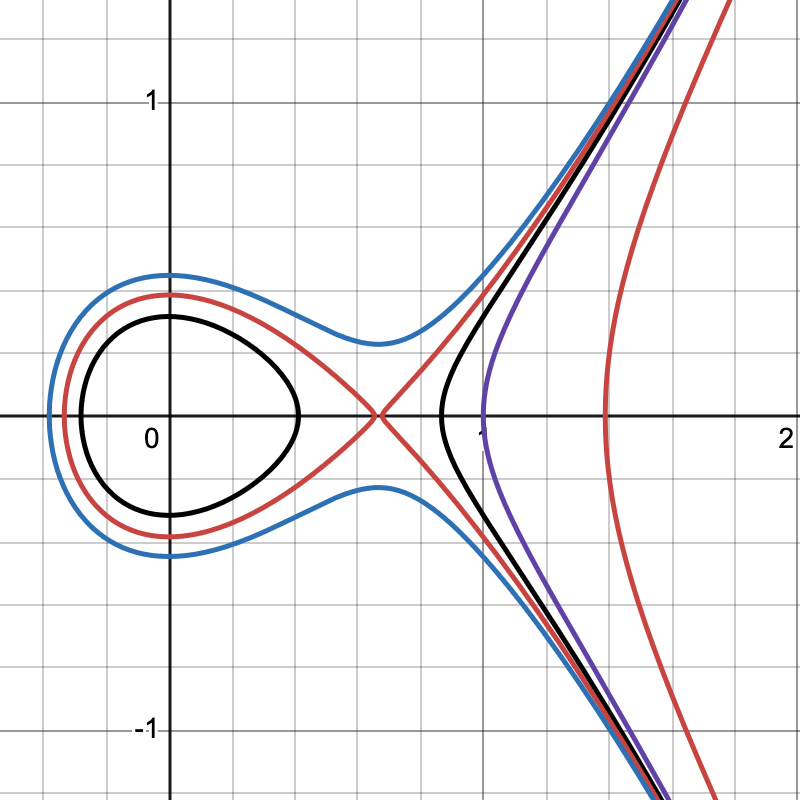
\includegraphics[height=5cm]{Grafico1}
	\end{center}
\end{sol}

\begin{oss}
	I punti di massimo e di minimo giocano un ruolo importante per quanto riguarda la velocità $v(x) = \sqrt{\frac 2m (E-V(x)}$.
\end{oss}

Bisogna sottolineare che tutte queste curve non sono altro che esemplificazioni, perché rappresentano intere regioni di spazio. Per esempio $E_1$ può essere apportata a qualsiasi valore negativo dell'energia.\\
Per ogni valore di $E$ abbiamo quindi un'orbita a sé stante, quindi il piano delle fasi non è altro che un piano riempito di curve.
Infatti, se prendessimo un qualsiasi punto $(x_0, v_0)$, abbiamo che esiste un'unica orbita che passi per quel punto. Se così non fosse infatti, avremmo che due si intersecano, quindi per due livelli di energia si avrà che in $x_0$ si avrà la stessa velocità, il che è assurdo in quanto abbiamo teoremi che ci assicurano l'unicità della curva.

Inoltre non ci devono essere degli spazi lasciati vuoti, infatti deve essere chiara la transizione tra le due orbite. Infatti ci sono dei valori particolari di $E$ che permettono di delimitare le aree. Queste linee prendono il nome di \textbf{Linee Separatorie}

\begin{ese}
	Fare la discussione alla Weierstrass per $U(x) = - (x^2-1)^2$
\end{ese}

\begin{sol}
	Iniziamo con lo scrivere la funzione $V$ dell'energia potenziale:
	\[ V(x) = (x^2-1)^2 \]
	Andiamo a fare uno studio veloce della funzione:
	\[ \lim_{x \to \pm \infty} V(x) = +\infty\qquad V(0) = 1 \]
	Calcolando la derivata prima (per trovare le condizioni di equilibrio) abbiamo che:
	\[ V'(x) = 4x(x^2-1) = 0 \qquad \Leftrightarrow \qquad x = 0\quad \vee x = \pm 1 \]
	Vedendo i segni, abbiamo che $\pm 1$ sono punti di minimo mentre $0$ è un punto di massimo. Graficamente abbiamo che:
	\begin{center}
		\begin{tikzpicture}[domain = -1.5:1.5]
			\draw[->] (-2,0) -- (2,0);
			\draw[->] (0,-1) -- (0,2);
			\draw[samples = 1000] plot (\x, {((\x)^2-1)^2});
			\draw[blue] (-2,0) -- (2,0) node[right]{$E_1$}
				(-2,0.5) -- (2,0.5) node[right]{$E_2$}
				(-2,1) -- (2,1) node[right]{$E_3$}
				(-2,1.5) -- (2,1.5) node[right]{$E_4$};
			\filldraw (-1,0) circle(1pt) node[below]{$-1$}
				(1,0) circle(1pt) node[below]{$1$}
				(-1.3,0.5) circle(1pt)
				(-1.3,0) circle(1pt)
				(-0.54,0.5) circle(1pt)
				(-0.54, 0) circle(1pt)
				(1.3,0.5) circle(1pt)
				(1.3,0) circle(1pt)
				(0.54,0.5) circle(1pt)
				(0.54, 0) circle(1pt)
				(-1.414,1) circle(1pt)
				(-1.414,0) circle(1pt)
				(0,1) circle(1pt) node[above right]{$1$}
				(0,0) circle(1pt)
				(1.414,1) circle(1pt)
				(1.414,0) circle(1pt)
				(-1.5,1.5) circle(1pt)
				(-1.5,0) circle(1pt)
				(1.5,1.5) circle(1pt)
				(1.5,0) circle(1pt);
			\draw[dotted] (-1.3,0.5) -- (-1.3,0)
				(1.3,0.5) -- (1.3,0)
				(-0.54,0.5) -- (-0.54,0)
				(0.54,0.5) -- (0.54,0)
				(-1.414,1) -- (-1.414,0)
				(1.414,1) -- (1.414,0)
				(-1.5,1.5) -- (-1.5,0)
				(1.5,1.5) -- (1.5,0);
			\draw (3.25,0.5) node{$\Rightarrow$};
			\draw (4,0) -- (8,0);
			\filldraw (5,0) circle(1pt) node[below]{$-1$}
				(7,0) circle(1pt) node[below]{$1$}
				(4.7,0) circle(1pt) node[above]{$x_1$}
				(5.46, 0) circle(1pt) node[above]{$_2$}
				(7.3,0) circle(1pt) node[above]{$x_4$}
				(6.54, 0) circle(1pt) node[above]{$x_3$}
				(4.596,0) circle(1pt) (4.596,0.75) node(5){$x_5$}
				(0,0) circle(1pt) node[below]{$0$}
				(7.414,0) circle(1pt) (7.414,0.75) node(6){$x_6$}
				(4.5,0) circle(1pt) (4.5,1.25) node(7){$x_7$}
				(7.5,0) circle(1pt) (7.5,1.25) node(8){$x_8$};
			\draw[dotted] (5) -- (4.596,0)
				(6) -- (7.414,0)
				(7) -- (4.5,0)
				(8) -- (7.5,0);
		\end{tikzpicture}
	\end{center}
	Calcoliamo quali possono essere i valori ammissibili:
	\[ \mathscr E : E \geq \inf_{x \in \mathbb R} V(x) = 0\qquad \Rightarrow \qquad \mathscr E = [0, +\infty[ \]
	Quindi $E$ non potrà mai assumere un valore negativo. I possibili valori sono:
	\begin{itemize}
		\item $E_1 = 0$, qui abbiamo due radici multiple
		\item $0<E_2<1$, qui abbiamo $4$ radici semplici
		\item $E_3 = 1$, qui abbiamo una radice multipla e due semplici
		\item $E_4>1$, qui abbiamo due radici semplici
	\end{itemize}
	Andiamo ad analizzare caso per caso (il grafico delle fasi sarà direttamente rappresentato a fine esercizio)

	\textbf{Caso $E_1 = 0$}\\
	In questo caso abbiamo che il dominio è:
	\[ D_1 = \{1,-1\} \]
	Abbiamo soltanto due punti, quindi $x_0 = 0$ oppure $x_0 = 1$. Stando in un contesto non relativistico, un punto non può passare da una posizione all'altra facendo salti, quindi intuitivamente il corpo resta fermo nella condizione di partenza. Più formalmente abbiamo che:
	\begin{itemize}
		\item Se $x_0 = 1$, possiamo dire che si tratti di un \textbf{Moto Stazionario} $x(t) = 1, \forall t \geq t_0$ in quanto $E_1 = V(1) = 0$, quindi ha velocità iniziale $v_0 = 0$. $1$ è una configurazione di equilibrio e $1$ è una radice multipla.
		\item Il discorso è analogo per quanto riguarda $x_0 = -1$, in quanto avendo sempre $E = V(-1) = 0$ e di conseguenza avendo anche che $v_0 = 0$, $x(t) = -1, \forall t \geq t_0$
	\end{itemize}

	\textbf{Caso $0<E_2<1$}\\
	Qui abbiamo che il dominio è:
	\[ D_2 = [x_1,x_2] \cup [x_3,x_4] \]
	Andiamo a vedere i singoli intervalli:
	\begin{itemize}
		\item Se ho che $x_0 \in [x_1,x_2]$, sicuramente ho che se $x_0 = -1$, la sua velocità è non nulla, visto che si ha una condizione di $v_0  = 0$ se e solo se il punto parte da $x_1$ o da $x_2$. Quindi possiamo trattare $x_0 = -1$ come con gli altri casi. Sappiamo poi che $x_1$ e $x_2$ sono due radici semplici, quindi sono due punti di inversione del moto. Quindi abbiamo un \textbf{Moto Periodico} tra le radici semplici $x_1$ e $x_2$
		\item Se $x_0 \in [x_3,x_4]$ allora la cosa è del tutto analoga, quindi ho un \textbf{Moto Periodico} di estremi le radici semplici $x_3$ e $x_4$
	\end{itemize}

	\textbf{Caso $E_3= 1$}\\
	Qui abbiamo che il dominio è definito da:
	\[ D_3 = [x_5,x_6] \]
	Questo è un caso completamente diverso da quello precedente, in quanto abbiamo anche il punto $0$ che è un radice multipla. Andiamo comunque a vedere i singoli casi, dando attenzione anche al singolo $x_0 = 0$
	\begin{itemize}
		\item Se $x_0 = 0$, abbiamo che $E = V(0) = 1$, per cui abbiamo che $v_0 = 0$. Da questo e dal atto che $x=0$ è una condizione di equilibrio, abbiamo che il punto \textbf{Resta Fermo} $x(t) = 0, \forall t \geq t_0$
		\item Se $x \in ]0, x_6]$, allora abbiamo che, essendo compreso tra una radice multipla $0$ ed una radice semplice $x_6$, abbiamo un \textbf{Moto Asintotico} verso $0$ se $v_0<0$ e un'\textbf{Inversione di Moto}, seguito poi da un \text{Moto Asintotico} verso $0$ per $v_0>0$.
		\item Se $x \in [x_5,0[$, in maniera analoga al punto precedente, abbiamo un \textbf{Moto Asintotico} verso $0$ per $v_0>0$ ed un'\textbf{Inversione di Moto} in $x_5$ seguita poi da un \textbf{Moto Asintotico} verso $0$ per $v_0<0$
	\end{itemize}

	\textbf{Caso $E_4>1$}\\
	Qui abbiamo che il dominio è:
	\[ D_4 = [x_7, x_8] \]
	Qui abbiamo un'unica condizione, che è quella $x_0 \in [x_7, x_8]$. Quindi, stando in mezzo a due radici semplici, abbiamo un \textbf{Moto Periodico} tra le radici semplici $x_7$ e $x_8$.

	Il Grafico delle Fasi sarà quindi

	\begin{center}
		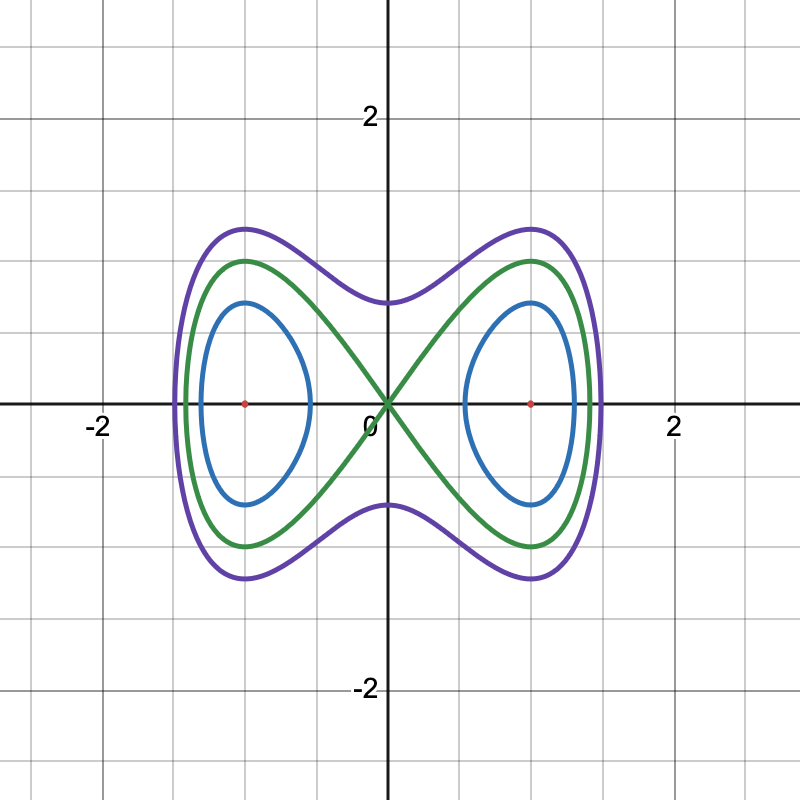
\includegraphics[height=5cm]{Grafico2}
	\end{center}
\end{sol}

\begin{ese}
	Fare la discussione alla Weierstrass per $V = -(x^2-1)^2$
\end{ese}

\begin{sol}
	Essendo questo un caso analogo a quello precedente, quindi daremo giusto un accenno di soluzione. Il suo grafico è:
	\begin{center}
		\begin{tikzpicture}[domain = -1.5:1.5]
			\draw[->] (-2,0) -- (2,0);
			\draw[->] (0,-2) -- (0,1);
			\draw[samples = 1000] plot (\x, {-((\x)^2-1)^2});
			\draw[blue] (-2,-1.5) -- (2,-1.5) node[right]{$E_1$}
				(-2,-1) -- (2,-1) node[right]{$E_2$}
				(-2,-0.5) -- (2,-0.5) node[right]{$E_3$}
				(-2,0) -- (2,0) node[right]{$E_4$}
				(-2,0.5) -- (2,0.5) node[right]{$E_5$};
		\end{tikzpicture}
	\end{center}
	Troviamo i valori ammissibili per $E$:
	\begin{itemize}
		\item $E_1 < -1$, dove abbiamo due radici semplici
		\item $E_" = -1$, dove abbiamo due radici semplici e una multipla
		\item $-1<E_3<0$, dove abbiamo $4$ radici semplici
		\item $E_4 = 0$, dove abbiamo due radici multiple
		\item $E_5>0$, dove non abbiamo radici
	\end{itemize}
	A fine esercizio, il suo piano delle fasi sarà:
	\begin{center}
		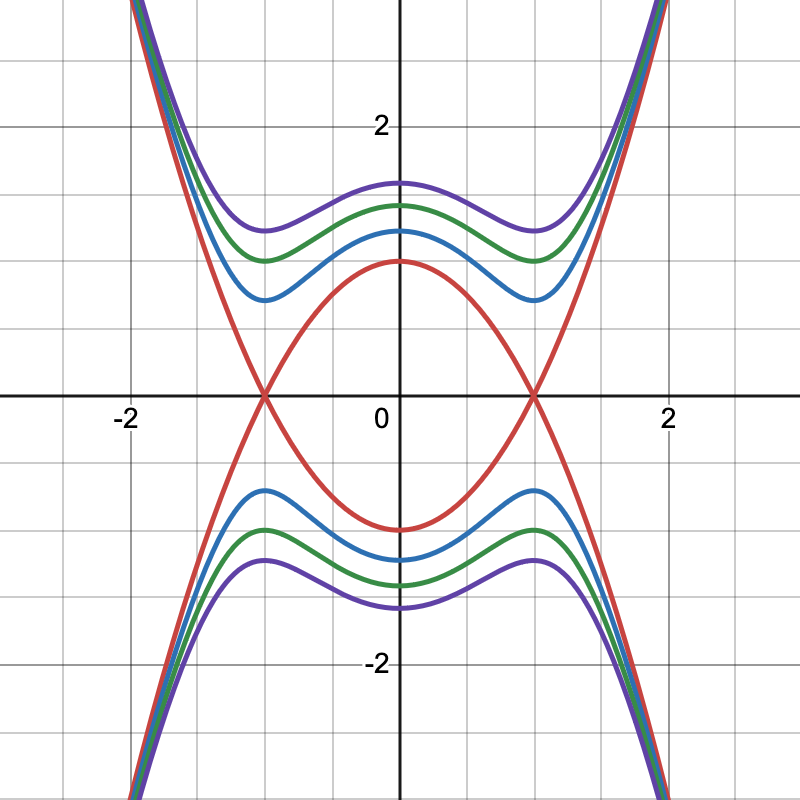
\includegraphics[height=5cm]{Grafico3}
	\end{center}
\end{sol}

\begin{ese}
	Fare la discussione alla Weierstrass per $U(x) = 2e^{-x^3} - e^{-2x^3+1}$
\end{ese}

\begin{sol}
	Cominciamo con il trovare l'Energia Potenziale:
	\[ V(x) = e^{-2x^3+1} - 2e^{-x^3} \]
	Facciamo uno studio di funzione rapido per carpirne il grafico:
	\[ \lim_{x \to +\infty} V(x) = 0 \qquad \lim_{x \to -\infty}V(x) = 0 \qquad V(0) = e-2\]
	Calcoliamone la derivata per trovare i punti critici:
	\[ V'(x) = -6x^2e^{-2x^3+1} + 6x^2e^{-x^3} = 6x^2 e^{-2^3+1} (-1 + e^{x^3-1}) \]
	Da cui segue che:
	\[ V'(x) = 0\qquad \Leftrightarrow \qquad x = 0\quad x = 1 \]
	Calcolando il valore della funzione in $1$ abbiamo che:
	\[ V(1) = -e^{-1} = -\frac 1e \]
	Quindi il suo grafico è:
	\begin{center}
		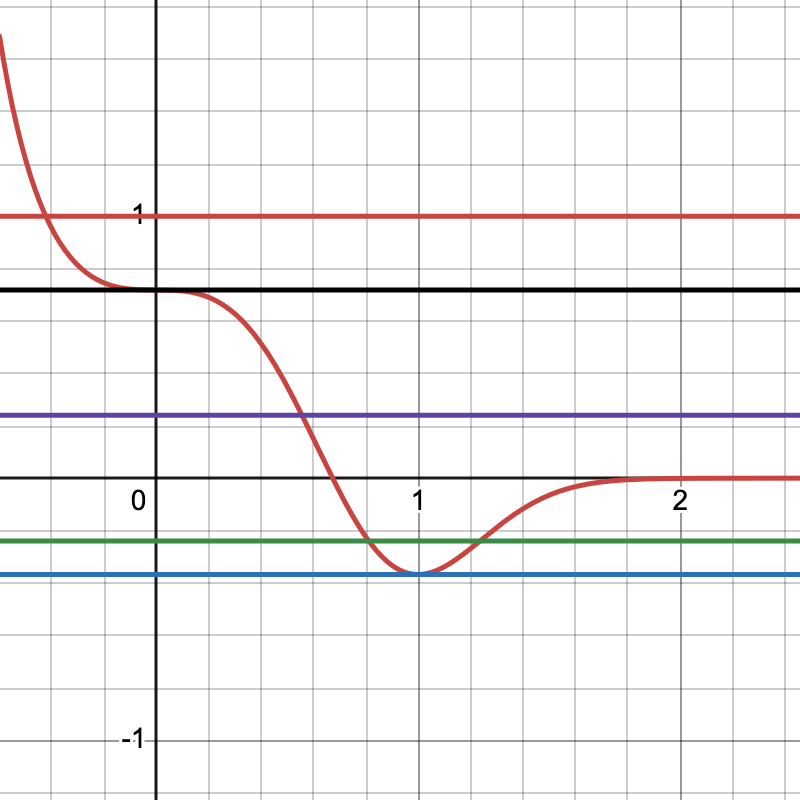
\includegraphics[height=5cm]{Grafico4}
	\end{center}
	I possibili valori di $E$ sono:
	\begin{itemize}
		\item $E_1= -\frac 1e = m_0$ dove abbiamo una radice multipla
		\item $m_0< E_2< 0$, qui abbiamo due radici semplici
		\item $E_3 = 0$ dove abbiamo una radice semplice
		\item $0<E_4<e-2$ dove abbiamo ancora una radice semplice
		\item $E_5 = e-2$ dove abbiamo una radice multipla
		\item $E_6 > e-2$ dove abbiamo una radice semplice
	\end{itemize}
	Notiamo che i casi con $E_3$ e $E_4$ possono essere raggruppati, però per il momento li possiamo considerare come due casi distinti

	\textbf{Caso $E_1 = -\frac 1e$}\\
	Qui abbiamo che il dominio possibile è:
	\[ D_1 = \{1\} \]
	Se $x_0 = 1$, abbiamo che $E_1 = V(1)$, per cui $v_0 = 0$. Allora abbiamo che $x(t) = 1$, $\forall t \geq t_0$, in quanto $1$ è una configurazione di equilibrio.

	\textbf{Caso $m_0 < E_2<0$}\\
	Il nostro dominio ora è:
	\[ D_2 = [x_1,x_2] \]
	Se $x \in [x_1,x_2]$, abbiamo che $x_0$ è compreso tra due radici semplici, per cui abbiamo un \textbf{Moto Periodico} tra $x_1$ e $x_2$

	\textbf{Caso $E_3 = 0$}\\
	Il nostro dominio qui è:
	\[ D_3 = [x_3, +\infty[ \]
	Sappiamo che $x_3$ è una radice semplice, per cui abbiamo un punto di inversione. Il moto è quindi un \textbf{Moto Aperiodico} a $+\infty$ e c'è un'\textbf{Inversione di Moto} in $x_3$ se $v_0<0$. Per capire come rappresentarlo nel piano delle fasi, dobbiamo calcolare il limite:
	\[ \lim_{x \to +\infty} v(x)= \lim_{x \to +\infty} \sqrt{\frac{2}{m} (E_3 - V(x)}) = 0 \]

	\textbf{Caso $0<E_4<e-2$}\\
	Il nostro dominio qui è:
	\[ D_4 = [x_4, +\infty[ \]
	Proprio come nel caso precedente (per questo si poteva unirli) abbiamo che $\forall x\geq x_4$ abbiamo un \textbf{Moto Aperiodico} a $+\infty$ (e abbiamo un'\textbf{Inversione di Moto} se $v_0<0$). Anche qui, se lo vogliamo rappresentarlo nel piano delle fasi, dobbiamo calcolare il limite:
	\[ \lim_{x \to +\infty} \pm \sqrt{\frac 2m(E_4 - V(x))} = \pm \sqrt{\frac 2m E_4} \]

	\textbf{Caso $E_5 = e-2$}\\
	Il nostro dominio è:
	\[ D_5 = [0,+\infty[ \]
	Diversamente dai casi precedenti abbiamo una radice multipla $0$. Distinguiamo i due casi:
	\begin{itemize}
		\item Se $x_0 = 0$, allora abbiamo che $E_5 = V(0)$, da cui segue che $v_0 = 0$, per cui $x(t) = 0, \forall t \geq t_0$ in quanto questa era una condizione di equilibrio.
		\item Se invece $x_0>0$ dobbiamo nuovamente distinguere i due casi. Se $v_0>0$ abbiamo un \textbf{Moto Aperiodico} verso $+\infty$ di cui il limite all'infinito è:
			\[ \lim_{x \to \infty}\pm \sqrt{\frac 2m E_5 - V(x)} = \pm \sqrt{\frac{2E_5}{m}} \]
			Altrimenti abbiamo un \textbf{Moto Asintotico} verso $0$
	\end{itemize}

	\textbf{Caso $E_6>e-2$}\\
	Come nel caso con $E_4$ e $E_3$, abbiamo un \textbf{Moto Aperiodico} verso $+ \infty$ con un'\textbf{Inversione di Moto} in $x_6$. Il suo limite all'infinito è:
	\[ \lim_{x \to +\infty} v(x) = \lim_{x \to +\infty}\pm \sqrt{\frac 2m E_6 - V(x)} = \pm \sqrt{\frac{2E_6}{m}} \]

	Il suo grafico delle fasi sarà quindi
	\begin{center}
		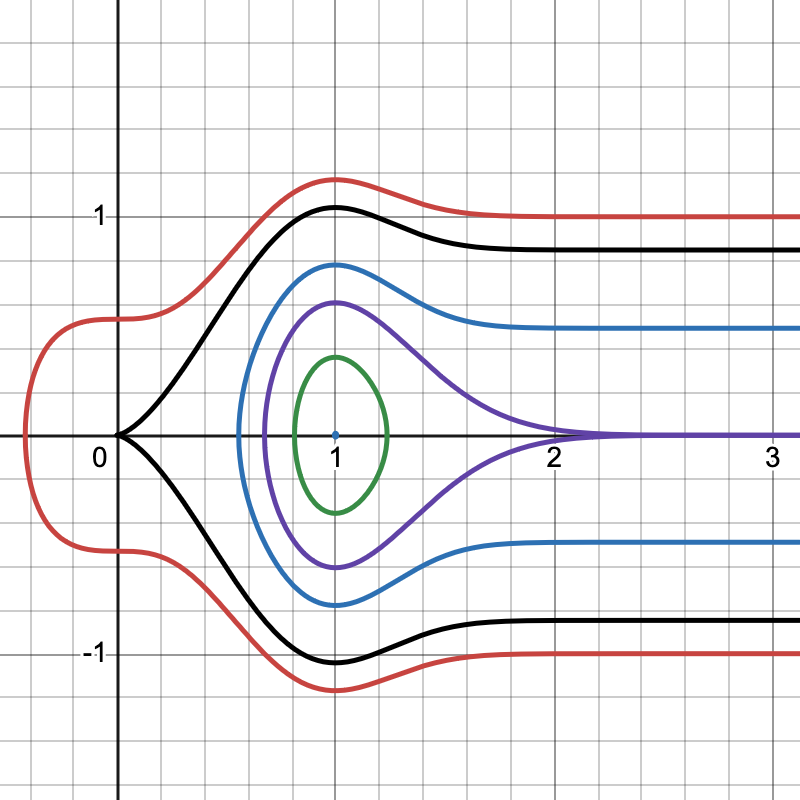
\includegraphics[height=5cm]{Grafico5}
	\end{center}
\end{sol}

Un esercizio che è stato dato:
\begin{ese}
	Fare la discussione di Weierstrass per $U = e^{-x} - e^{-2x}$
\end{ese}

\newpage

\section{Moti Unidimensionali Speciali}

In questo capitolo tratteremo di moti unidimensioanli speciali, nei quali è possibile poter dire di più rispetto all'analisi qualitativa di Weierestrass

\subsection{Solo Forza Elastica}

Supponiamo di avere un muto, che si muove lungo un asse e su di esso ci agisce una forza elastica di vettore $\vec F = -k^2x \mathbf i$:
\begin{center}
	\begin{tikzpicture}
		\draw[->] (0,0) -- (4,0) node[right]{$x$};
		\filldraw (0.5,0) circle(1pt) node[above]{$P$}
			(0,0) circle (1pt) node[above]{$O$};
	\end{tikzpicture}
\end{center}
Conoscendo la forza, possiamo calcolare anche il potenziale e l'energia potenziale:
\[ U(x) = -\frac{k^2x^2}2 \qquad \text e \qquad V(x) = \frac{k^2x^2}2 \]
Graficamente abbiamo che:
\begin{center}
	\begin{tikzpicture}[domain = -1.5:1.5]
		\draw[samples = 1000] plot(\x, {(\x)^2});
		\draw[->] (-2,0) -- (2,0);
		\draw[->] (0,-0.5) -- (0,3);
		\draw[blue] (-2,0) -- (2,0) (-2,1) -- (2,1);
		\filldraw (1,1) circle(1pt) (1,0) circle(1pt) node[below]{$x_2$} (-1,1) circle(1pt) (-1,0) circle(1pt) node[below]{$x_1$};
		\draw[dotted] (1,1) -- (1,0) (-1,1) -- (-1,0);
	\end{tikzpicture}
\end{center}
Se abbiamo che $E_1 = 0$, allora si ha che l'unica posizione possibile è $x_0 = 0$, che è una configurazione di equilibrio stabile. Se invece $E_2>0$, allora sappiamo che il punto è situato tra due radici semplici, per cui abbiamo un moto Periodico tra le due radici.

Il suo piano delle fasi sarà:
\begin{center}
	\begin{tikzpicture}[domain = -2:2]
			\begin{scope}[decoration={
				markings,
				mark=at position 0.5 with {\arrow{>}}}]
				\draw[samples = 500, blue, postaction = {decoration}] plot ({\x}, {sqrt(1 - (0.5*\x)^2)});
			\end{scope}
		\draw[samples = 500, blue] plot ({\x}, {-sqrt(1 - (0.5* \x)^2)});
		\draw[->] (-3,0) -- (3,0);
		\draw[->] (0,-1.5) -- (0,1.5);
		\filldraw[green] (0,0) circle(1pt);
	\end{tikzpicture}
\end{center}

Però questo è un caso facile, quindi volendo saremmo in grado di dire di più. In questo caso potremmo fare una descrizione dal punto di vista quantitativo.
Recuperiamo la legge di Newton:
\[ m\ddot x = R_x \qquad \Rightarrow \qquad m\ddot x - k^2 x\]
Se poi poniamo:
\[ \omega^2 = \frac{k^2}m \qquad \Rightarrow \qquad \ddot x + \omega^2 x = 0\]

Per poter avanti, introduciamo dei concetti di analisi
\textit{
	\begin{defn}{Equazione Differenziale del Secondo Ordine Lineare}{}
		Si definisce \textbf{Equazione Differenziale del Secondo Ordine Lineare Omogenea a Coefficienti costanti} un'equazione differenziale del tipo:
		\[ \ddot x + a_1\dot x + a_0 x = 0 \]
		Dove $a_1,a_2 \in \mathbb R$
	\end{defn}
	L'incognita da trovare è una funzione $x = x(t)$ con $t\geq t_0$. Nel caso presentato presentato precedentemente abbiamo che $a_1 = 0$ e $a_0 = \omega^2$.\\
	Volendo è possibile mettere un coefficiente davanti a $\ddot x$, ma se è nullo, la nostra equazione non può essere di secondo grado, essendo quindi il primo grado il grado più alto. Inoltre, se è uno scalare qualsiasi, lo possiamo dividere affinché sia $1$.}

\textit{Definiamo con $S$:
	\[ S = \{x(t): x\text{ è una soluzione dell'equazione differenziale}\} \]
	Possiamo dimostrare che $S$ è uno spazio vettoriale di dimensione $2$ sul campo $\mathbb K$ (può essere $\mathbb C$ oppure $\mathbb R$). Il fatto che sia di dimensione $2$ che ci basta trovare due soluzioni linearmente indipendenti per trovare una base, quindi per trovare tutte le soluzioni di tale equazione differenziale. In particolare, se $\{x_1,x_2\}$ è una base di $S$:
	\[ x(t) = c_1x_1(t) + x_2x_2(t) \qquad \forall c_1,c_2 \in \mathbb K \]
}
\textit{
	Come si risolve un'equazione differenziale?
	\begin{defn}{Equazione Associata ad un'Equazione Differenziale}{}
		Sia $\ddot x + a_1 \dot x + a_0 x = 0$ un'equazione differenziale lineare di secondo ordine omogenea, allora si definisce \textbf{Equazione Associata all'Equazione Differenziale} l'equazione in $\lambda$:
		\[ \lambda^2 + a_1 \lambda + a_0 = 0 \]
		In particolare, ci basta sostituire $\lambda^k$ come parametro con $k$ corrispondente all'ordine di derivazione della funzione incognita.
	\end{defn}
	\begin{prop}{}{}
		Se $\lambda$ è soluzione di $\lambda^2 + a_1 \lambda + a_0 = 0$, equazione associata ad un'equazione differenziale lineare di secondo ordine omogenea, allora $x(t) = e^{\lambda t}$ è soluzione di tale equazione differenziale
	\end{prop}
	Siamo cercando una base, cosa che si traduce con il cercare due valori soltanto. Vediamo i possibili casi:}
\begin{itemize}
	\item \textit{Se le due radici $\lambda_1, \lambda_2 \in \mathbb R$ sono distinte, allora abbiamo che le due soluzioni:
		\[ x_1 = x_1(t)\qquad x_2 = x_2(t) \]
		sono due soluzioni distinte e linearmente indipendenti, quindi rappresentano una base, infatti:
		\[ c_1e^{\lambda_1t} + c_2 e^{\lambda_2t} = 0\qquad \Leftrightarrow \qquad c_1 = c_2 = 0 \]
		La più generale soluzione dell'equazione differenziale $\ddot x + a_1 \dot x + a_0x =0$ del tipo:}
		\[ x(t) = c_1e^{\lambda_1t} + c_2 e^{\lambda_2t} \qquad \forall c_1,c_2 \in \mathbb K \]
		\textit{In particolare, ponendo:}
		\[
			\begin{cases}
				x(t_0) = c_1 e^{\lambda_1 t_0} + c_2 e^{\lambda_2 t_0} = x_0\\
				\dot x(t_0) = c_1 \lambda_1 e^{\lambda_1 t_0} + c_2 \lambda_2 e^{\lambda_2 t_0} = \dot x_0
			\end{cases}
		\]
		\textit{Da qui si possono trovare $c_1$ e $c_2$ per trovare la soluzione desiderata.}
	\item \textit{Se le due radici sono coincidenti, abbiamo che $\lambda_1 = \lambda_2 = \lambda$, per quanto fatto prima abbiamo che $x_1(t) = e^{\lambda t}$ è una soluzione dell'equazione differenziale. Però per trovare una base ce ne servono due. Volendo è possibile dimostrare che anche $x_2(t) = te^{t \lambda}$ è una soluzione a tale equazione differenziale. Perciò abbiamo ottenuto la base $\{e^{\lambda t}, te^{\lambda t}\}$. Quindi possiamo scrivere una generica equazione come:
		\[ x(t) = c_1e^{\lambda t} + c_2t e^{\lambda t}\qquad \forall c_1,c_2 \in \mathbb K \]
		Per trovare una soluzione precisa, ci basta porre un sistema simile a quello precedente.}
	\item \textit{Nel caso in cui abbiamo $2$ radici complesse coniugate, allora:
		\[ \text{se }\lambda_{1,2} = p \pm iq \qquad p,q \in \mathbb R, q \neq 0\]
		Allora abbiamo che le soluzioni sono:
		\[ x_1(t) = e^{\lambda_1t} \qquad \text{e} \qquad x_2(t) = e^{\lambda_2t} \]
		Per quanto visto nel primo caso, queste sono due soluzioni linearmente indipendenti, quindi le soluzioni generali sono del tipo:
		\[ x(t) = c_1e^{\lambda_1 t} + c_2 e^{\lambda_2 t} \qquad \forall x_1,c_2 \in \mathbb K\]
		Però questi sono valori complessi che spiegano un movimento reale. Sfruttiamo l'identità di Eulero, allora otteniamo che:
		\[ \begin{cases}
			x_1(t) = e^{pt} \cdot e^{iqt} = e^{pt}(\cos(pt) + i \sin(qt))\\
			x_2(t) = e^{pt}\cdot e^{-iqt} = e^{pt}(\cos(pt) - i\sin(1t))\\
		\end{cases}\]
		Per cui, ponendo $y_1$ $y_2$ come:
		\[ y_1 = \frac{x_1 + x_2}2 = e^{pt}\cos(qt)\qquad \text e \qquad y_2 = \frac{x_1-x_2}{2i} = e^{pt}\sin(qt) \]
		Queste sono due soluzioni dell'equazione differenziale e valori reali e sono due valori linearmente indipendenti, quindi $\{y_1, y_2\}$ è una base di $S$. La più generale soluzione sarà quindi:
		\[ x(t) = c_1e^{pt}\cos(qt) + x_2e^{pt}\sin(qt)\qquad \forall c_1,c_2 \in \mathbb R \]
		Possiamo fare delle sostituzioni del tipo:
		\[\begin{cases}
			c_1 = c\cos \gamma\\
			c_2 = -c\sin \gamma
		\end{cases} \qquad \Leftrightarrow \quad \begin{cases}
			c = \sqrt{c_1^2 + c_2^2}\\
			\gamma = -\arctan (\frac{c_2}{c_1})
		\end{cases}\]
	In questo modo la soluzione generale diventa:}
	\[ x(t) = ce^{pt}\cos(qt) \cos\gamma - ce^{pt}\sin(qt)\sin \gamma = ce^{pt}\cos(qt + \gamma)\qquad \forall c, \gamma \in \mathbb R\]
\end{itemize}

Quindi, avevamo che la nostra equazione era:
\[ \ddot x + \omega^2 x = 0 \quad \Rightarrow \quad \lambda^2 + \omega^2 = 0\quad \Rightarrow\quad \lambda_{1,2} = i\omega \]
Usando la formula appena trovata con $p = 0$ e $q = \omega$, abbiamo che:
\[ x(t) = c\cos(\omega t + \gamma)\qquad \forall x,\gamma \in\mathbb R \]
Questo è uno dei moti che avevamo trovato precedentemente nel capitolo \ref{2.2}. In particolare questo si tratta di un \textbf{Moto Oscillatorio Periodico} di periodo $T = \frac{2\pi}\omega$. Ovviamente, con la discussione qualitativa avevamo già trovato il fatto che fosse periodico, così sappiamo qualcosa in più.

\subsection{Forza Elastica e Resistenza del Mezzo}

In questo caso, sul punto agiscono due forze di vettori $\vec F = -k^2x \mathbf i$ e $\vec F_1 = -2pm \dot x \mathbf i$ con $p>0$ detto \textbf{Coefficiente di Resistenza del Mezzo}.
\begin{center}
	\begin{tikzpicture}
		\draw[->] (0,0) -- (4,0);
		\filldraw (0,0) circle(1pt) node[below]{$O$} (1,0) circle(1pt) node[below]{$P$};
	\end{tikzpicture}
\end{center}
Questo è un caso che non può esser trattato con un'analisi qualitativa alla Weierstrass, in quanto non tutte le forze sono conservative (quella di resistenza per esempio, in quanto non è neanche posizionale). Continua però a valere la legge di Newton, per cui sappiamo che vale:
\[ m\ddot x = -2pm \dot x - k^2 x \]
In particolare, ponendo:
\[\omega^2 = \frac{k^2}m>0 \quad \Rightarrow \quad \ddot x + 2p \dot x + \omega^2x = 0\]
In questo caso abbiamo che $a_1 = 2p$ e $a_2 = \omega^2$. Quindi segue che:
\[ \lambda^2 + 2p\lambda + \omega^2 = 0\quad \Rightarrow \quad \lambda_{1,2} = -p \pm \sqrt{p^2-\omega^2} \]
A seconda del rapporto che c'è tra $p$ e $w$, ci sono tre possibili casi:
\begin{itemize}
	\item Se ho che $p^2>\omega^2$, allora ho due radici reali distinte, entrambe negative. Per evidenziare il fatto che sono negative, possiamo scriverle come:
		\[ \lambda_i = - \beta_i \qquad \Rightarrow \qquad \beta_i = -\lambda_i > 0 \]
		Per cui abbiamo che la soluzione è diventata:
		\[ x(t) = c_1e^{\lambda_1t} + c_2e^{\lambda_2t} = c_1e^{-\beta_1t} + c_2e^{-\beta_2t} \qquad \forall c_1,c_2 \in \mathbb R\]
		Si tratta quindi di un \textbf{Moto Smorzato}, in quanto abbiamo la condizione che:
		\[ \lim_{t \to 0}s(t) =0 \]
		Quindi assume la forma di un \textbf{Moto Aperiodico Smorzato}
	\item Se ho che $p^2 = \omega^2$, allora ho che $\lambda_1,2 = -\beta<0$. In questo caso, abbiamo che la base $\{ e^{-\beta t}, te^{-\beta t} \}$. Quindi la soluzione generale è:
		\[ x(t) = c_1 e^{-\beta t} + c_2 t e^{-\beta t}\qquad \forall c_1,c_2 \in \mathbb R \]
		Si tratta quindi di un \textbf{Moto Smorzato con Smorzamento Critico}
	\item Se abbiamo che $p^2< \omega^2$, allora possiamo chiamare per comodità la quantità $p^2 - \omega^2 = -q^2 <0$. Per cui abbiamo che $\lambda_{1,2} = -p \pm iq$. In questo modo abbiamo che la soluzione generale è:
		\[ x(t) = ce^{-pt}\cos(qt + \gamma) \qquad \forall c, \gamma\in \mathbb R\]
		Quindi abbiamo un \textbf{Moto Oscillatorio Smorzato}
\end{itemize}
Quello che accomuna questi tre casi è che abbiamo sempre un moto smorzato.

\subsection{Con 3 Forze}

Analizziamo adesso il caso in cui agiscono una forza elastica, la forza di resistenza del moto e una forza di tipo sinusoidale. Allora abbiamo che le forze hanno vettore rispettivamente:
\[ \vec F = -k^2 x \mathbf i\qquad \vec F_1 = 2pm\dot x \mathbf i \qquad \vec F_2 = A \cos (\Omega t + \gamma)\mathbf i \]
Dove $\Omega, A,\gamma \in \mathbb R$ e senza perdere di generalità $A>0$. Come nel caso precedente, non possiamo fare lo studio alla Weiersrtass, in quanto $F_1$ e $F_2$ non sono conservative.\\
Sappiamo che continua a valere il il secondo principio della dinamica, quindi continua a valere:
\[ m\ddot x = -2pm \dot x + A \cos(\Omega t + \gamma) \]
Se poi poniamo $\omega^2 = \frac{K^2}m$ e $N = \frac Am$, allora abbiamo che:
\[ \ddot x = 2p\dot x + \omega^2 x = N\cos (\Omega t+\gamma) \]

Questo tipo di equazione differenziale prende il nome di \textbf{Equazione Differenziale Lineare di Secondo Ordine non Omogenea}.
\textit{
	\begin{defn}{Equazione Diff. Lineare di Secondo Ordine non Omogenea}{}
		Si definisce un'\textbf{Equazione Differenziale Lineare di Secondo Ordine non Omogenea} un'equazione differenziale del tipo:
		\[ \ddot x + a_1 \dot x + a_0 x = f(x) \neq 0 \]
	\end{defn}
}
Volendo è possibile dimostrare che:
\begin{prop}{}{}
	La più generale soluzione di $\ddot x + a_1 \dot x + a_0 x = f(x)$ è della forma:
	\[ x(t) = x_0(t) + x_1(t) \]
	Dove $x_0(t)$ è la soluzione più generale dell'equazione omogenea associata a $\ddot x + a_1 \dot x + a_0 x = f(x)$, cioè $\ddot x + a_1 \dot x + a_0 x = 0$, mentre $x_1(t)$ è una soluzione particolare dell'equazione differenziale stessa
\end{prop}

Analizziamo per bene questo risultato. Abbiamo che $x_1(t)$ genera comunque un moto smorzato (stando a esattamente quanto visto in precedenza), quindi abbiamo che:
\[ \lim_{t \to +\infty}x_0(t) = 0 \]
$x_1(t)$ invece è una soluzione particolare. Quindi il problema si è spostato da trovare una soluzione generale a trovare una soluzione in base alla situazione in cui siamo. Infatti, sapendo che $x_0$ è un moto smorzato, possiamo approssimare $x(t)$ come:
\[ x(t) \approx x_1(t)\qquad \text{per }t \to +\infty \]

Per trovare un caso particolare, consideriamo un'equazione ausiliaria del tipo:
\[ \ddot z + 2p \dot z + \omega^2z = Ne^{i(\Omega t + \alpha)} \]
Se troviamo le soluzioni di questa e ne prendiamo solamente la parte reale, abbiamo trovare la soluzione del nostro problema di partenza.\\
In particolare, è possibile dimostrare che:

\begin{prop}{}{}
	Se $z(t)$ è soluzione di $\ddot z + 2p \dot z + \omega^2z = Ne^{i(\Omega t + \alpha)}$, allora:
	\[\Re(z(t)) \text{ è soluzione di }\ddot x + a_1 \dot x + a_0 x = f(x)\]
\end{prop}

Questa non è altro che una semplificazione del problema, in quanto possiamo scrivere:
\[ Ne^{i(\Omega t+ \alpha)} = Ne^{i \alpha} e^{i \Omega t} \]
In particolare, ponendo $n = Ne^{i \alpha} \in \mathbb C$ tale che $N = |n|$ e $arg(n) = \alpha$, possiamo trasformare:
\[ \ddot z + 2p \dot z + \omega^2z = Ne^{i(\Omega t + \alpha)} \qquad \Leftrightarrow \qquad \ddot z+ 2p \dot z + \omega^2z = ne^{i \Omega t} \]
Dimostriamo ora la proposizione:

\begin{proof}
	Supponiamo l'equazione $\ddot z + 2p \dot z + \omega^2z = Ne^{i(\Omega t + \alpha)}$, allora abbiamo che:
	\begin{align*}
		\Re(\ddot z(t)) + 2p \Re(\dot z(t)) + \omega^2 \Re(z(t)) &= N \cos(\Omega t + \alpha)\\
		(\Re (z(t)))\;\ddot{} + 2p(\Re(z(t)))\;\dot{} + \omega^2 \Re(z(t)) &= N\cos(\Omega t + \alpha)\\
		\ddot x(t) + 2p \dot x(t) + \omega^2 x(t) x(t) &= N\cos(\Omega t + \alpha)
	\end{align*}
\end{proof}

Cerchiamo quindi una soluzione di $\ddot z + 2p \dot z + \omega^2z = Ne^{i(\Omega t + \alpha)}$ che sia della forma:
\[ z(t) = Ce^{i (\Omega t + \gamma)} \]
Per appropriati $C, \gamma \in \mathbb R$. Ma questo è equivalente a chiedere che:
\[ z(t) = Ce^{i\gamma}e^{i \Omega t} = ce^{i\Omega t}\]
Dove abbiamo posto che $c = Ce^{i \gamma}$. Se quindi la soluzione ha questa forma, allora le sue derivate sono:
\[ \dot z(t) = ic\Omega e^{i \Omega t}\qquad \ddot z(t) = -c\Omega^2 e^{i \Omega t} \]
Per cui, andando a sostituire, abbiamo che:
\begin{align*}
	-c\Omega^2 e^{i \Omega t} + 2pic\Omega e^{i \Omega t} + \omega^2 ce^{i \Omega t} &= ne^{i \Omega t} \quad \forall t \in \mathbb R\\
	c(-\Omega^2 + 2pi\Omega + \omega^2) = n
\end{align*}
Da cui segue direttamente che:
\[ c = \frac{n}{\omega^2 - \Omega^2 + 2\pi\Omega} \in \mathbb C \]
Questa è la nostra soluzione complessa. Cerchiamo quindi $C$ e $\gamma$:
\[ C = |c| = \frac{N}{\sqrt{(\omega^2-\Omega^2) + (2p\Omega)}} \qquad \text e \qquad n = arg(c)\]
Quindi, tornando al problema originario, abbiamo che:
\[ x_1(t) = C \cos (\Omega t + \gamma) \]
È una soluzione particolare al problema originale, quella a cui tendono tutte le altre soluzioni. Quindi il punto si muoverà di \textbf{Moto Oscillatorio Armonico}. Quindi la soluzione $x(t)$ può essere approssimata come:
\[ x(t) \approx C\cos(\Omega t + \gamma) \]
Il punto quindi subisce le \textbf{Oscillazioni Forzate} indotte dalla forza esterna che subisce con la stessa periodicità $T = \frac{2 \pi}{\Omega}$.
Volendo possiamo stimare come variano tali oscillazioni in particolare studiando come varia $C = C(\Omega) = f(\Omega^2)$, cioè possiamo studiare quanto questa funzione raggiunge i livelli massimi. Definiamo:
\[ g(\Omega^2) = (\omega^2- \Omega^2) + 4 p^2\Omega^2 \]
Per trovare il massimo delle oscillazioni, dobbiamo trovare quando $g$ è minima, quindi, andando a calcolare la derivata, abbiamo che:
\[ g'(\Omega^2) = -2(\omega^2 - \Omega^2) + 4p = 0 \qquad \Leftrightarrow \qquad \Omega^2 = \omega^2 - 4p\]
Nella maggior parte dei casi, abbiamo che $p$ è trascurabile rispetto agli altri parametri, per cui abbiamo un massimo delle oscillazioni quando $\Omega^2 \approx \omega^2$, cioè quando $\Omega \approx \omega$, cioè quando la frequenza delle oscillazioni forzate approssima la frequenza delle oscillazioni proprie. Quando questo si verifica, si può parlare di \textbf{Risonanza}.

\begin{es}
	Fu proprio quest'effetto che fece crollare il ponte di Tacana
\end{es}

\subsection{Dinamica del Pendolo Matematico}

Avevamo già introdotto il pendolo matematico in precedenza (basta riprendere l'esercizio \ref{pendolo}) per cui abbiamo che:
	\begin{center}
		\begin{tikzpicture}
			\draw[dashed] (0,0.5) -- (0,-2.5);
			\draw (330:2) arc(330:240:2cm) (0,0) -- node[pos = 0.5,above]{$\ell$} (315:2) (270:0.5) arc (270:315:0.5) node[pos =0.3, below right]{$\theta$};
			\filldraw (0,0) circle(1pt) node[above right]{$O$} (0,-2) circle(1pt) node[below right]{$O_1$} (315:2) circle(1pt) node[below right]{$P$};
			\draw[->] (315:2) -- ++ (0,-1) node[right]{$m\vec g$};
			\draw[->, blue] (315:2) -- ++ (0.5, 0.5) node[right]{$\vec t$};
			\draw[->, blue] (315:2) -- ++ (-0.5, 0.5) node[below]{$\vec n$};
		\end{tikzpicture}
	\end{center}
Sapevamo già che ci bastava un solo parametro lagrangiano $n = 1$ per descrivere il moto del pendolo e che questo era $q=\theta$. Sapevamo anche già che le configurazioni di equilibrio sono $\theta_1 = 0$ e $\theta_2 = \pi$.\\
Introduciamo un sistema di coordinate intrinseche, allora abbiamo che:
\[ m\vec a = \vec F + \vec \Phi \]
Dove:
\[ s = \ell\theta \qquad \dot s = \ell \dot \theta \qquad \ddot s = \ell \ddot \theta \]
L'accelerazione può essere scritta come:
\[ \vec a = \ddot s \vec t + \frac{\dot s}{\rho_C}\vec n = \ell \ddot \theta \vec t + \ell \dot\theta^2 \vec n \]
Sapendo che agisce solamente la forza peso, abbiamo che:
\[ m\vec g = -mg\sin \theta \vec t - mg \cos \theta \vec n \]
Per trovare le componenti della reazione vincolare ci basta porre il sistema:
\[\begin{cases}
	mg\ell \ddot \theta = -mg \sin \theta\\
	m\ell \dot \theta^2 = -mg\cos \theta + \Phi_n\\
	0 = \Phi_b
\end{cases}\]
Sapendo però che la posizione dipende solamente dall'angolo $\theta$, possiamo ricavare l'angolo dalla prima, per poi metterlo nella seconda:
\[ \Phi_n = mg \cos \theta + m\ell \dot\theta^2 \]
In particolare quindi, andando a sviluppare la prima, abbiamo che:
\[ \ddot \theta = -\frac g \ell \sin \theta \qquad \Leftrightarrow \qquad \ddot \theta = -\omega^2 \sin \theta \qquad \text{con }\omega^2 = \frac g\ell \]

\textbf{Nel caso delle piccole oscillazioni}, cioè nel caso in cui $\theta<1$, possiamo approssimare $\sin \theta \approx \theta$, per cui abbiamo che:
\[ \ddot \theta = -\omega^2 \theta \qquad \Rightarrow \qquad \ddot \theta + \omega^2 \theta = 0 \]
Questa è un'equazione differenziale lineare omogenea ad incognita $\theta$.
La sua equazione associata è $\lambda^2 + \omega^2 = 0$, da cui segue che $\lambda_{1,2} = \pm i \omega$. Per cui la soluzione è:
\[ \theta (t) = C\cos (\omega t + \gamma) \qquad \text{con }T = \frac{2\pi}\omega = 2 \pi \sqrt{\frac \ell g} \]
Si tratta comunque di un moto oscillatorio armonico. In particolare, in questo caso specifico vale la \textbf{Legge dell'Isocronismo del Pendolo}, secondo cui il periodo del pendolo non dipende dalla massa di esso e non dipende dalle condizioni iniziali.

\textbf{Nel caso generale}, possiamo sfruttare la legge di conservazione dell'energia:
\[ \frac 12 mv^2 + V(\theta) = E \]
Cerchiamo quindi, come prima cosa, di determinare l'energia potenziale:
\[ U = -mgy = -mg\ell (1-\cos \theta) \]
Sapendo poi che $v = |\dot s| = \ell |\dot \theta|$, abbiamo che:
\[ \frac 12 m\ell^2 \dot \theta^2 + mg\ell (1-\cos \theta) = E \]
Per poterla risolvere, ci servono le condizioni iniziali $\theta(t_0) = \theta_0$ e $\dot\theta(t_0) = \dot \theta_0$. A questo punto possiamo andare a sostituire per ottenere $E$. Notiamo che questa è un'equazione differenziale del primo ordine, quindi:
\begin{align*}
	\dot \theta^2 &= \frac{2E}{m\ell^2} - \frac{2g}{\ell}(1-\cos \theta)
\end{align*}
Tuttavia, ponendo e sapendo che:
\[ \omega^2 = \frac g \ell\qquad \text e \qquad \sin \frac \theta 2 = \frac{1-\cos \theta}2 \]
Otteniamo che:
\begin{align*}
	\dot \theta^2 &= \frac{2E}{m\ell^2} - \frac{2g}{\ell}(1-\cos \theta) = \frac{2E}{mg} - 4 \omega^2 \sin^2 \frac \theta 2 = 4\omega^2 \left( \frac{E}{2mg\ell} - \sin^2\frac \theta 2 \right)
\end{align*}
Per cui abbiamo che:
\[ \frac{\dot \theta}2 = \pm \sqrt \omega{\frac{E}{2mg\ell} - \sin^2\frac \theta 2} = \pm \sqrt \omega{f\left(\frac \theta 2\right)}\]
Se poi poniamo $x = \frac \theta 2$, otteniamo esattamente:
\[ \dot x = \pm \omega \sqrt{f(x)} \]
Che è esattamente quanto avevamo trovato per la discussione alla Weiersrtass. Quindi possiamo proseguire con tale discussione adesso. Quindi, ponendo:
\[ E' = \frac E{2mg \ell} \]
I possibili valori che $E'$ può assumere sono:
\begin{itemize}
	\item $E'>1$
	\item $E' = 1$
	\item $E'<1$
\end{itemize}

\textbf{Caso $E'>1$}\\
In questo caso abbiamo che $E>2mg\ell$, per cui:
\[ \frac E{2mg\ell} - \sin^2 \frac \theta 2\text{ non si annulla mai}\]
Cioè abbiamo che:
\[ f\left(\frac \theta 2\right) \neq 0 \qquad \Rightarrow \qquad v\left(\frac \theta 2\right) \neq 0\]
In questo caso il moto non è Aperiodico a $+\infty$, in quanto non può andare all'infinito, ma si tratta di \textbf{Moto Rivolutivo} (in senso orario o antiorario a seconda delle condizioni iniziali)

\textbf{Caso $E'=1$}\\
A questo caso corrisponde:
\[ E=2mg\ell \qquad \Rightarrow \qquad f\left(\frac {\theta}{2} \right) = 1-\sin^2\frac \theta 2 \]
Quindi abbiamo che:
\[ f\left(\frac \theta 2\right) =0 \qquad \Leftrightarrow \qquad \sin^2\frac \theta 2 = 1 \qquad \Leftrightarrow \qquad \theta = \pm \pi\]
\begin{center}
	\begin{tikzpicture}
		\draw (0,0) circle(1cm) (0,0) -- (0,-1) (0,0) -- (-60:1);
		\filldraw (0,0) circle(1pt) (-60:1) circle(1pt);
		\draw[dashed] (0,0) -- (0,1);
		\draw[->] (0,-0.5) arc (-90:90:0.5cm) node[pos = 0.5, right]{$\pi$};
		\draw[->] (0,-0.5) arc (270:90:0.5cm) node[pos =0.5, left]{$-\pi$};
	\end{tikzpicture}
\end{center}
Ma $\pm \pi$ sono radici semplici o muliple? Studiando la derivata prima, abbiamo che:
\[ f'\left(\frac \theta 2\right) = 2 \sin \frac \theta 2 \cos  \frac \theta 2 \]
Poiché anche la derivata prima si annulla in $\pm \pi$, segue che sono radici multiple. Quindi, da qualunque configurazione iniziale, il punto si mette in modo dirigendosi verso le radici multiple, che raggiunge in un tempo infinito. Si tratta quindi di un \textbf{Moto Asintotico Verso $\pm \pi$} (a seconda appunto del segno di $v_0$)

\textbf{Caso $E'<1$}.\\
In questo caso abbiamo che:
\[ E<2mg\ell \qquad \Rightarrow \qquad \frac E{2mg \ell}<1 \qquad \Leftrightarrow \qquad \frac{E}{2mg\ell} = \sin^2\frac \alpha 2 \]
Da cui segue banalmente che:
\[ \alpha = 2 \arcsin \sqrt{\frac E{2mg\ell}} \]
Questo è un dato noto, in quanto conosciamo tutte le quantità $E,m,g,\ell$. A questo punto abbiamo che:
\[ f\left( \frac \theta 2 \right) = \sin^2\frac \alpha 2 - \frac \theta 2 = 0 \qquad \Leftrightarrow \qquad \sin^2 \theta \frac 2 = \sin^2 \frac \alpha 2 \qquad \Leftrightarrow \qquad \theta = \pm \alpha \]
\textit{Ma queste sono radici semplici o multiple?} Possiamo dire con certezza che queste sono radici semplici in quanto sappiamo che le sole $\theta = 0$ e $\theta = \pi$ sono radici multiple. Quindi si tratta di radici semplici, quindi il punto si muove di \textbf{Moto Periodico tra} $-\alpha$ e $\alpha$. Ci troviamo quindi in un caso più generale di quello delle piccole oscillazioni.

\newpage

\section{Dinamica Relativa del Punto Materiale}

Abbiamo già visto nel capitolo \ref{Relativo} tutto quello che riguarda i moti relativi rispetto a moti di riferimento differenti. Cerchiamo quindi di apportarli a sistemai di forze
\begin{center}
	\begin{tikzpicture}
		\draw[->] (0,0) -- (2,0) node[right]{$y$};
		\draw[->] (0,0) -- (0,2) node[left]{$z$};
		\draw[->] (0,0) -- (-1,-1) node[left]{$x$};
		\draw[->, thick] (0,0) -- (1,0) node[above]{$\mathbf j$};
		\draw[->] (0,0) -- (0,1) node[left]{$\mathbf k$};
		\draw[->] (0,0) -- (-0.5,-0.5) node[above left]{$\mathbf i$};
		\draw[->] (4,0) -- (5,1) node[right]{$y$};
		\draw[->] (4,0) -- (3,1) node[left]{$z$};
		\draw[->] (4,0) -- (4.5,-1.5) node[left]{$x$};
		\draw[->, thick] (4,0) -- (4.5,0.5) node[above]{$\mathbf j$};
		\draw[->] (4,0) -- (3.5,0.5) node[left]{$\mathbf k$};
		\draw[->] (4,0) -- (4.25,-0.75) node[above left]{$\mathbf i$};
		\filldraw (0,0) circle(1pt) node[below]{$O$} (4,0) circle(1pt) node[below right]{$O_1$} (2,1.5) circle(1pt) node[above]{$P$};
	\end{tikzpicture}
\end{center}
Dal teorema di Coriolis \ref{Coriolis}.4 avevamo che:
\[ \vec a = \vec a_1 + \vec a_\tau + \vec a_C \]
Quindi lo possiamo portare alle forze. In tal caso abbiamo che:
\[ m\vec a = m\vec a_1 + m\vec a_\tau + m\vec a_c \]
Visto che siamo in un contesto relativo (vedere il capitolo \ref{qta}), possiamo dire che tutte queste sono forze. In particolare quindi possiamo dire che:
\[ m\vec a_1 = \vec F_1 + \vec\Phi_1 \qquad \text e \qquad m\vec a = \vec F + \vec \Phi\]
Tuttavia, avevamo che le reazioni vincolari erano invarianti per sistema di riferimento, da cui $\vec \Phi_1 = \vec \Phi$. Per cui possiamo scrivere (a meno di semplificazioni) che:
\[ \vec F_1 = \vec F - m\vec a_\tau - m\vec a_c \]
Dove $m\vec a_\tau$ rappresenta la \textbf{Forza di Trascinamento}, mentre $m\vec a_c$ rappresenta la \textbf{Forza di Coriolis}. Da queste otteniamo:
\[ m\vec a_1 = \vec F - m\vec a_\tau - m\vec a_c \]
Da questo possiamo studiare le forze nel sistema relativo conoscendo quelle nel sistema assoluto. Vediamone dei casi particolari:

\subsection{Forza Peso}

Sappiamo che la forza peso è quella forza che agisce su un punto posto sulla superficie terrestre dalla terra stessa. In particolare sappiamo anche che tale punto è fermo rispetto alla Terra stessa.\\
In generale abbiamo che
\begin{center}
	\begin{tikzpicture}
		\draw[->] (0,0) -- (2,0) node[right]{$y$};
		\draw[->] (0,0) -- (0,2) node[left]{$z$};
		\draw[->] (0,0) -- (-1.4,-1.4) node[left]{$x$};
		\filldraw (0,0) circle(1pt) node[below]{$(S)$} (2,1) circle(1pt) node[below]{$O$} (4,2) circle(1pt) node[right]{$P$};
		\draw[dashed] (2,1) -- (4,2);
		\draw[->] (2,1) -- node[pos = 0.5, above]{$\vec r$} (2.5,1.25);
		\draw[->] (4,2) -- node[pos = 0.5, below]{$\vec F$} (3.5,1.75);
	\end{tikzpicture}
\end{center}
Dove abbiamo che su $P$ agisce una forza:
\[ \vec F = -K \frac{mM}{\rho^2}\vec r \]
Mentre su $O$, per principio di azione e reazione, agisce una forza $-\vec F$.\\
Andando a studiare il caso in cui il punto sta sulla superficie abbiamo che:
\begin{center}
	\begin{tikzpicture}
		\draw[->] (0,0) -- (2,0) node[right]{$y$};
		\draw[->] (0,0) -- (0,2) node[left]{$z$};
		\draw[->] (0,0) -- (-1.4,-1.4) node[left]{$x$};
		\filldraw (0,0) circle(1pt) node[below]{$(S)$} (2,2) circle(1pt) node[below]{$O$} (2,2) ++ (30:1) node(p){} circle(1pt) node[right]{$P$};
		\draw (2,2) circle(1cm);
	\end{tikzpicture}
\end{center}
A questo punto possiamo dare la definizione di Peso effettiva:

\begin{defn}{Peso}{}
	Il \textbf{Peso} è la forza attrattiva esercitata dalla massa terrestre su un punto $P$ vista dal punto di vista di un osservatore solidale con la superficie terrestre
\end{defn}

Andiamo a studiare quindi la formula del peso:
\[ \vec P = \vec F_1 = \vec F - m\vec a_\tau - m\vec a_c \]
In questo caso particolare, sappiamo quanto vale il raggio e vale quanto il raggio terrestre $R$. Per cui abbiamo che che:
\[ \vec F = -K\frac{mM}{R^2}\vec r \]
Andiamo a studiare le altre forze:\\
Sappiamo che il punto nel sistema assoluto non è fermo, in quanto ruota prima attorno al sole e con esso si sposta nella via lattea. Però stando al sistema di riferimento della terra, esso è solidale, quindi $\vec v_1 = 0$, da cui segue che:
\[ \vec a_c = 2 \vec \omega \times \vec v_1 = 0 \qquad \Rightarrow \qquad m\vec a_c = 0 \]
Per studiare l'accelerazione di trascinamento, andiamo a fare delle considerazioni. Sappiamo che la terra ruota sul proprio asse, quindi il punto sulla sua superficie compie rotazioni su una circonferenza di raggio minore:
\begin{center}
	\begin{tikzpicture}
		\draw (-2.5,0) -- (2.5,0);
		\draw (0,-2.5) -- (0,2.5);
		\draw (0,0) circle(2cm);
		\draw (2,0) arc (0:-180:2cm and 0.5cm);
		\draw[dashed] (2,0) arc(0:180: 2cm and 0.5cm);
		\draw (0,0) -- (45:2);
		\draw (45:2) arc(0:-180:1.414cm and 0.3cm);
		\draw[dashed] (45:2) arc(0:180:1.414cm and 0.3cm);
		\filldraw (45:2) circle(1pt) node[right]{$P$} (0,1.414) circle(1pt)node[left]{$H$};
		\draw (45:2) -- node[pos = 0.5, below]{$\rho_C$} (0,1.414);
		\draw (0.5,0) arc (0:45:0.5) node[pos = 0.5,right]{$\varphi$};
	\end{tikzpicture}
\end{center}
In particolare possiamo dire che il raggio della circonferenza su cui si muove è $\rho_C = R \cos \varphi$. Si tratta quindi di un moto di rotazione, in cui possiamo prendere:
\[ s_\tau = \rho_C\theta  \qquad \dot s_\tau = \rho_C\dot \theta = \rho_C \omega \qquad \ddot s_\tau = \rho_C \ddot \theta = \rho_C \dot \omega \]
Ma in questo caso la velocità angolare della terra è costante, quindi $\dot \theta = 0$, per cui $\ddot s_\tau = 0$. Da questo segue che:
\[ \vec a_\tau = \ddot s_\tau \vec t + \frac{\dot s_\tau^2}{\rho_C} \vec n = \rho_C \omega^2 \cos \varphi \vec n \]
\begin{center}
	\begin{tabular}{|c|}
		\hline
		\textbf{Attenzione:} I versori $\vec n$ e $\vec t$ sono sulla circonferenza di raggio $\rho_C$\\
		Non sulla circonferenza grande di raggio $R$\\
		\hline
	\end{tabular}
\end{center}
Da questo segue che:
\[ \vec P = \vec F_1 = \vec F - mR\omega^2 \cos \varphi \vec n \qquad \text{con }\vec F = -K\frac{mM}{R^2}\vec r\]
Per cui abbiamo che la forza peso è leggermente deviata rispetto alla normale:
\begin{center}
	\begin{tikzpicture}
		\draw (2,0) arc (0:90:2cm);
		\filldraw (1.414,1.414) circle(1pt) node[right]{$P$};
		\draw[dashed] (0,0) -- (1.414,1.414);
		\draw[->] (1.414,1.414) -- (1.212,1);
	\end{tikzpicture}
\end{center}
Conoscendo questa formula della forza peso, possiamo calcolare in quali punto della superficie terrestre si ha una forza peso maggiore e dove una minore:
\[ \vec P_{\max} = \cos \varphi = 0 \quad \Leftrightarrow \quad \varphi = \pm \frac \pi 2 \qquad \text e \qquad \vec P_{\min} = \cos \varphi= 1 \quad \Leftrightarrow \quad \theta = 0\]

\begin{oss}
	Noi di solito scriviamo la forza peso come $\vec P = m\vec g$. Ma da dove salta fuori? Sappiamo che:
	\[ \vec P = \vec F_1 - m\vec a_1 = -K\frac{mM}{R^2}\vec r - m\omega^2 R \cos \varphi \vec n \]
	Da cui si ottiene che:
	\[ \vec a_1 = -K\frac{M}{R^2}\vec r - \omega^2 R \cos \varphi \vec n \]
	Visto che non dipende più dal punto (se non in minima parte, che è sostanzialmente trascurabile), possiamo chiamare tale accelerazione $\vec g$
\end{oss}

\subsection{Problema dei Due Corpi}

Supponiamo di avere un sistema solidale $(S)$ e due punti $O$ e $P$ con massa rispettivamente $M$ e $m$.
\begin{center}
	\begin{tikzpicture}
		\draw[->] (0,0) -- (2,0) node[right]{$y$};
		\draw[->] (0,0) -- (0,2) node[left]{$z$};
		\draw[->] (0,0) -- (-1.4,-1.4) node[left]{$x$};
		\filldraw (0,0) circle(1pt) node[below]{$(S)$} (2,1) circle(1pt) node[below]{$O$} (4,2) circle(1pt) node[right]{$P$};
		\draw[dashed] (2,1) -- (4,2);
		\draw[->] (2,1) -- node[pos = 0.5, above]{$\vec r$} (2.5,1.25);
		\draw[->] (4,2) -- node[pos = 0.5, below]{$\vec F$} (3.5,1.75);
	\end{tikzpicture}
\end{center}
Sappiamo che su $P$ agisce una forza di vettore $\vec F$:
\[ \vec F = -K\frac{mM}{\rho^2}\vec r \]
E sappiamo sempre che, per il principio di azione e reazione, abbiamo che su $O$ agisce $-\vec F$.\\
Nel sistema assoluto sappiamo trovare le posizioni dei punti, utilizzando le rispettive leggi dei moti:
\[ m\vec a = \vec F \qquad \text e \qquad M \vec a_O = - \vec F \]

Il problema dei due corpi sta nel fatto di determinare il moto di un punto $P$ rispetto al sistema relativo con origine nel punto $O$ e che trasla rispetto a $(S)$

\begin{center}
	\begin{tikzpicture}
		\draw[->] (0,0) -- (2,0) node[right]{$y$};
		\draw[->] (0,0) -- (0,2) node[left]{$z$};
		\draw[->] (0,0) -- (-1.4,-1.4) node[left]{$x$};
		\filldraw (0,0) circle(1pt) node[below]{$(S)$} (2,1) circle(1pt) node[below left]{$O$} (4,2) circle(1pt) node[right]{$P$};
		\draw[dashed] (2,1) -- (4,2);
		\draw[->] (2,1) -- node[pos = 0.5, above]{$\vec r$} (2.5,1.25);
		\draw[->] (4,2) -- node[pos = 0.5, below]{$\vec F$} (3.5,1.75);
		\draw[->] (0.5,1) -- (4,1);
		\draw[->] (2,0.5) -- (2,3);
	\end{tikzpicture}
\end{center}
\textit{Questo tipo di problema può essere paragonato a quello di trovare il moto dei pianeti rispetto al sole}\\
Sappiamo che rispetto a $(O)$, abbiamo che:
\[ m \vec a_1 = \vec F - m\vec a_\tau - m\vec a_c \]
Queste due ultime quantità sono proprio quelle che vogliamo trovare.\\
Però $\vec a_c$ non ci da problemi, in quanto abbiamo che il moto è di traslazione, quindi $\vec \omega = 0$, quindi:
\[ \vec a_c = 2 \vec \omega \times \vec v_1 = 0 \]
Anche $\vec a_\tau$ non ci da problemi. Infatti, essendo $\vec a_\tau$ l'accelerazione che il punto avrebbe se fosse solidale con il sistema di riferimento ed essendo il moto un moto di traslazione, abbiamo che:
\[ \vec a_\tau (P) = \vec a_O = -\frac {\vec F}M \]
Per cui otteniamo che:
\[ m\vec a_1 = \vec F + m \frac{\vec F}M = \frac{m+M}M \vec F= \vec F_1 \]
In questo modo abbiamo che la forza $\vec F_1$ è un multiplo della forza $\vec F$ nel sistema assoluto, però mantiene stessa direzione e lo stesso verso. Infatti:
\[ \|\vec F\| = \|\vec F\|\cdot \frac{m+M}M > \|\vec F\| \qquad \Rightarrow \qquad m\vec a_1 = \vec F_1\]
Volendo lo possiamo vedere anche in un altro modo:
\[ m\vec a_1 = \frac{m+M}M \vec F_1 \quad \Rightarrow \quad \frac{Mm}{m+M}\vec a_1 = \mu \vec a_1 = \vec F_1 \]
Possiamo chiamare la quantità $\mu$ come \textbf{Massa Ridotta}, in quanto possiamo affermare con certezza che $\mu<M$. Quindi otteniamo la legge:
\[ \mu \vec a_1 = \vec F \]
Quindi rispetto al sistema $(O)$, il punto $P$ è come se si muovesse con la stessa forza $\vec F$ presente in $(S)$, ma è come se avesse una massa $\mu$ minore.

Per il sistema relativo abbiamo quindi che:
\begin{center}
	\begin{tikzpicture}
		\draw[->](-1,0) -- (3,0);
		\draw[->](0,-1) -- (0,3);
		\filldraw (0,0) circle(1pt) node[below right]{$O$} (2,1) circle(1pt) node[right]{$P$};
		\draw[dashed] (0,0) -- (2,1);
		\draw[->] (2,1) -- (1.5,0.75) node[above]{$\vec F$};
	\end{tikzpicture}
\end{center}
Calcoliamo il momento delle forze $K$:
\[ \vec K_1 (O) = m\vec v \times (O-P) \]
Trovandone la derivata e sapendo che il punto $O$ è fermo, abbiamo che:
\[ \left. \frac{d \vec K_1(O)}{dt}\right|_{(O)} = m\vec a_1 \times (O-P) - m\vec v_1 \times \vec v_1 m\vec a_1 = \vec F \times (O-P) = 0\]
\textit{Si annulla tutto in quanto sono tutti vettori paralleli}. Visto, quindi, che la derivata è nulla, abbiamo che $\vec K_1(O)$ è costante nel tempo. In particolare, i vettori $O-P$ e $m\vec v_1$ determinano un piano, al quale $\vec K_1(O)$ deve rimanere ortogonale. Si tratta quindi di un moto piano. Quindi possiamo passare alle coordinate polari.
\begin{center}
	\begin{tikzpicture}
		\draw (0,0) -- (3,0);
		\draw (0,2) to[out = 30, in = 90] (30:2) to[out = -90, in = 180] (3,-0.5);
		\draw (0,0) -- node[pos = 0.5, above]{$\rho$} (30:2);
		\draw[blue,->] (0,0) -- node[pos = 0.5, above]{$\vec t$} (30:1);
		\draw[blue,->] (0,0) -- node[pos = 0.5, left]{$\vec h$} (120:1);
		\draw (0.5,0) arc (0:30:0.5) node[pos = 0.5,right]{$\theta$};
	\end{tikzpicture}
\end{center}
Conosciamo la traiettoria $\rho = \rho(\theta)$ e conosciamo il moto $\rho = \rho(t)$ e $\theta = \theta (t)$. Quindi:
\[ \mu(a_\rho \vec r + a_\theta \vec h) = -K \frac{mM}{\rho^2}\vec r\]
Tuttavia, sappiamo che $\vec r$ e $\vec h$ sono due vettori linearmente indipendenti, quindi sicuramente abbiamo che $a_\theta = 0$. Ma se $a_\theta = 0$, allora sappiamo con certezza che la velocità areolare $S'$ è costante e sappiamo che:
\[ S' = \frac 12 \rho^2 \dot \theta \]
Per cui vale la \textbf{Prima legge di Keplero}, cioè "vengono percorse aree uguali in tempi uguali":
\begin{center}
	\begin{tikzpicture}
		\draw (0,0) circle(3 and 2);
		\begin{scope}
			\clip (1,0) -- (2,2) -- (3,2) -- (3,-2) --(2,-2) -- (1,0);
			\filldraw[cyan] (0,0) circle(3 and 2);
		\end{scope}
		\begin{scope}
			\clip (1,0) -- (-3,1) -- (-3,-1) -- (1,0);
			\filldraw[cyan] (0,0) circle(3 and 2);
		\end{scope}
		\filldraw (1,0) circle(1pt) node[below]{$P$};
	\end{tikzpicture}
\end{center}
Per la formula di Binet, sappiamo che:
\[ a_\rho = -\frac{c^2}{\rho^2}\left( \frac{d^2 \frac 1 \rho}{d\theta^2 + \frac 1\rho} \right) \]
Se conosciamo la traiettoria, possiamo trovare tutto. \textit{Però è proprio quello che dobbiamo trovare}. Se poniamo:
\[ \frac c2 = S' = \frac 12 \rho^2 \dot \theta \]
Otteniamo che:
\[ \mu a_\rho \vec r = -K\frac{mM}{\rho^2}\vec r \]
Da cui otteniamo che:
\[ \frac{mM}{m+M} \left(-\frac{c^2}{\rho^2}\right)\left( \frac{d^2 \frac 1 \rho}{d \theta^2} \right) = -K\frac{mM}{\rho^2} \]
Da cui:
\[ \frac{d^2\frac 1\rho}{d \theta^2} + \frac 1 \rho = K\frac{m+M}c^2 \]
Se poniamo questa quantità come $\frac 1P$, otteniamo che:
\[ \frac{d^2\frac 1\rho}{d \theta^2} + \frac 1 \rho = \frac 1P\]
In particolare, se poniamo $\theta = t$ e $\frac 1 \rho = x$, otteniamo sostanzialmente che l'equazione differenziale appena trovata è:
\[ \frac{d^2x}{dt^2} + x = \frac 1\rho \]
In questo modo abbiamo una equazione differenziale lineare non omogenea. In questo modo avremo che la sua soluzione sarà della forma:
\[x(t) = x_0(t) + x_1(t)\]
Dove $x_0(t)$ è la soluzione dell'equazione differenziale lineare omogenea associata, mentre $x_1(t)$ è una soluzione particolare del problema dato.
\begin{itemize}
	\item Per la prima risolviamo l'equazione associata $\lambda^2 + 1 = 0$, da cui $\lambda_{1,2} = \pm i$, per cui le soluzioni dell'equazione differenziale omogenea sono:
		\[ x_0(t) = A\cos (t + \theta_0) \qquad A, t_0 \in \mathbb R \]
	\item Per l'equazione particolare abbiamo che una soluzione è:
		\[ x_1(t) = \frac 1P \qquad \Rightarrow \qquad \dot x_1 = \ddot x_1 = 0\]
		Per cui questa rappresenta una soluzione in quanto:
		\[ 0 + \frac 1P = \frac 1P \qquad \forall t \in \mathbb R \]
\end{itemize}
Per cui la nostra soluzione è:
\[ x(t) = A \cos (t + t_0) + \frac 1P = \qquad \Leftrightarrow \qquad \frac 1\rho(\theta) = A \cos(\theta + \theta_0) = \frac 1P\]
Questa è la nostra soluzione generale. In particolare, invertendola, otteniamo che:
\[ \rho(\theta) = \frac P{1 + A P \cos(\theta + \theta_0)}\qquad \forall A,\theta_0 \in \mathbb R \]
Questo ci serve per studiare il moto di un punto $P$ rispetto ad un punto $O$. Per esempio con le leggi di Keplero: la cosa ci può tornare utile per individuare la traiettoria $\rho=\rho(\theta)$. In particolare, se poniamo:
\[ e = -AP \qquad \Rightarrow \qquad \frac P{1 - e\cos(\theta-\theta_0)} \]

\begin{defn}{Eccentricità di una Curva}{}{}
	La quantità $|e| = |AP|$ prende il nome di \textbf{Eccentricità della Curva}. In particolare essa è legata al parametro $P$ ed è un termine generalmente noto.
	A seconda del valore dell'eccentricità si possono avere diverse curve:
	\begin{itemize}
		\item Se $|e|<1$ allora si ha un'ellisse (come nel caso dei pianeti)
		\item Se $|e|=1$ si ha una parabola (come nel caso di alcune parabole)
		\item Se $|e|>1$ in questo caso si ha un'iperbole
	\end{itemize}
\end{defn}

\begin{thm}{Terza Legge di Keplero}{}
	La terza legge di Keplero dice che:
	\[ \text{la quantità } \frac{T^2}{a^3} \text{ è costante} \]
\end{thm}

Notiamo che questa legge ci da una relazione tra $P = \frac {b^2}a$, dove $b$ e $a$ sono rispettivamente il semiasse minore e il semiasse maggiore.\\
\textit{Come possiamo calcolare il periodo di rotazione?} Se conosciamo:
\[ \frac c2 T = \pi ab \qquad \Rightarrow \qquad T = \frac{2 \pi ab}c \qquad \Rightarrow \qquad T^2 = \frac{4 \pi^2 a^2 b^2}{c^2} \]
In questo modo otteniamo che:
\[ \frac{T^2}{a^3} = \frac{4 \pi^2 a^2 b^2}{c^2 a^3} = \frac{4\pi^2 P}{c^2} = \frac{4 \pi^2}{K(m+M)} \]
\textit{A che cosa ci serve questo risultato?} Il rapporto resta comunque costante anche se gli oggetti variano:
\[ T^2 = \left[ \frac{4 \pi^2}{k(m+M)} \right] a^3\]
Il rapporto, infatti, resta lo stesso e varia solamente al variare dei pianeti (per la presenza della massa $m$ nella formula). Tuttavia, sapendo che $m<<M$, cioè che la massa del pianeta è molto inferiore rispetto a quella del sole, possiamo scrivere:
\[ \frac{T^2}{a^3} = \frac{4 \pi^2}{kM(1+\frac mM)} \approx \frac{4 \pi^2}{KM} \]
Da cui segue che il rapporto è quasi costante al variare dei pianeti.

\newpage

\section{Dinamica dei Sistemi Meccanici}

\subsection{Prime Definizioni}

Sia il corpo $\mathscr C$ costituito da $N$ punti $P_1,...,P_N$ con le rispettive masse $m_1,...,m_N$, le rispettive velocità $\vec v_1,...,\vec v_N$ e le rispettive accelerazioni $\vec a_1,...,\vec a_N$

\begin{defn}{Quantità di Moto del Corpo}{}
	Si definisce la \textbf{Quantità di Moto del Corpo} la quantità:
	\[ \vec Q = \sum_{s = 1}^N m_s \vec v_s \]
\end{defn}

\begin{prop}{}{}
	Sia dato un generico sistema di riferimento (fissato in partenza). Allora si ha che:
	\[ \vec Q = M\vec v_G \]
	Dove si ha che $M$ è la massa del copro e $\vec v_G$ è la velocità del baricentro.
\end{prop}
\begin{proof}
	Posto $(O) = (O,x,y,z)$, rispetto a $G$ abbiamo che:
	\[ G-O = \frac 1M \sum_{s = 1}^N m_s(P_s-O) \]
	Da cui segue che:
	\[ \sum_{s = 1} m_s(P_s - O) = M(G_O) \]
	Derivando a questo punto rispetto a $t$ abbiamo che:
	\[ \sum_{s = 1}^N m_s \vec v_s = M\vec v_G \qquad \Rightarrow \qquad \vec Q = M \vec v_G \]
\end{proof}

\begin{defn}{Momento delle Quantità di Moto rispetto ad un polo}{}
	Definiamo il \textbf{Momento delle Quantità di Moto rispetto ad un polo} $O \in \mathbb R^3$ il vettore:
	\[ \vec K(O) = \sum_{s = 1}^N m_s \vec v_S \times (O-P_S) \]
\end{defn}

\begin{defn}{Energia Cinetica del Corpo}{}
	Si definisce \textbf{Energia Cinetica del Corpo} la quantità:
	\[ T = \frac 12 \sum_{s = 1}^N m_Sv_s^2 + \]
\end{defn}

\begin{thm}{di König}{}\label{Konig}
	Rispetto ad un qualunque sistema di riferimento, per qualunque corpo, su ha il seguente risultato:
	\[ T = \frac 12 Mv_G^2 + T_G \]
	Dove $T_G$ è l'energia cinetica del corpo rispetto al sistema di riferimento \textbf{Baricentrico} che ha origine in $G$ e che trasla rispetto al sistema di riferimento $(O)$, $M$ è la massa totale del corpo e $\vec v_G$ è la velocità del baricentro
\end{thm}
\begin{proof}
	Se volessimo rappresentare la situazione, avremmo che:
	\begin{center}
		\begin{tikzpicture}
			\draw[->] (0,0) -- (2,0) node[right]{$y$};
			\draw[->] (0,0) -- (0,2) node[left]{$z$};
			\draw[->] (0,0) -- (-1,-1) node[left]{$x$};
			\draw[->, thick] (0,0) -- (1,0) node[above]{$\mathbf j$};
			\draw[->] (0,0) -- (0,1) node[left]{$\mathbf k$};
			\draw[->] (0,0) -- (-0.5,-0.5) node[above left]{$\mathbf i$};
			\draw[->] (2,1) -- (4,1) node[right]{$y'$};
			\draw[->] (2,1) -- (2,3) node[left]{$z'$};
			\draw[->] (2,1) -- (1.25,0.25) node[left]{$x'$};
			\draw[->, thick] (2,1) -- (3,1) node[above]{$\mathbf j$};
			\draw[->] (2,1) -- (2,2) node[left]{$\mathbf k$};
			\draw[->] (2,1) -- (1.5,0.5) node[above left]{$\mathbf i$};
			\filldraw (0,0) circle(1pt) node[below]{$O$} (2,1) circle(1pt) node[below right]{$G$} (4,2) circle(1pt) node[above]{$P_s$};
		\end{tikzpicture}
	\end{center}
	Noi vogliamo quanto calcolare quanto valga:
	\[ T = \frac 12 \sum_{s = 1}^N m_s v_s^2 \]
	Dove $\vec v_s = \vec v(P_s)$ è la velocità rispetto al sistema $(O)$, cioè la velocità vista nel sistema fermo. Possiamo prendere $\vec v_{1,s} = \vec v_1(P_s)$ le rispettive velocità relative. Allora l'energia cinetica in questo sistema è:
	\[ T_G = T_1 = \frac 12 \sum_{s = 1}^N m_{1,s} v_{1,s}^2\]
	Per il teorema di composizione delle velocità, abbiamo che:
	\[ \vec v_s = \vec v_{1,s} + \vec v_{\tau, s}\]
	Ma il sistema baricentrico non è un sistema qualunque, è quello che tiene fermo il baricentro. Inoltre, sapendo che il sistema $(G)$ trasla rispetto al sistema $(O)$, abbiamo che tutti i punti $P_s$ sono fermi rispetto al baricentro. Quindi, nel sistema assoluto tutti i punti hanno la stessa velocità. Da cui segue che:
	\[ \vec v_{\tau,s} = \vec v_G\]
	Facendo i conti espliciti abbiamo che:
	\begin{align*}
		T &= \frac 12 \sum_{s =1}^N m_s v_s^2 = \frac 12 \sum_{s =1}^N m_s(\vec v_{1,s} + \vec v_G)^2= \\
		&= \frac 12 \sum_{s = 1}^N m_s v_{1,s}^2 + \frac 12 \sum_{s = 1}^N m_s v_G^2 + \sum_{s = 1}^N m_s \vec v_{1,s}\cdot \vec v_{G}\\
		&= T_G + \frac 12 Mv_G^2 + \left(\sum_{s=1}^N m_s \vec v_{1,s}\right)\cdot \vec v_G
	\end{align*}
	Mostriamo che quest'ultimo termine della somma è nullo. Notiamo che il termine dentro alle parentesi corrisponde all'energia cinetica vista nel sistema di riferimento $(G)$, cioè:
	\[ \vec Q_1 = M\vec v_{1,G} \]
	E questa quantità è nulla per i commenti fatti in precedenza, quindi abbiamo che:
	\[ T_G = \frac 12 Mv_{G}^2 \]
\end{proof}

\subsection{Casi Particolare per il Calcolo dell'Energia}

In diversi casi, studiare l'energia rispetto a $(G)$ è più semplice rispetto a uno qualunque. Vediamo adesso dei casi particolari per il calcolo dell'energia.
\begin{itemize}
	\item Moto Traslatorio
	\item Moto Rotatorio
	\item Moto Rototraslatorio
\end{itemize}

\textbf{Moto Traslatorio}\\
In questo caso abbiamo che tutti i punti hanno la stessa velocità:
\[ \vec v_s = \vec v_G \qquad \forall s \in \{1,...,N\} \]
In questo caso abbiamo che:
\[ T = \frac 12 \sum_{s = 1}^N m_s v_s^2 = \frac 12 \left(\sum_{s = 1}^N m_s\right) v_G^2 = \frac 12 Mv_G^2\]
Con il teorema di König avremo avuto che $T_G = 0$

\textbf{Moto Rotatorio}\\
Prendiamo un generico punto $P_s$, allora abbiamo che:
\[ \forall P,O_1 \in \mathscr C \qquad \vec v(P) = \vec v(O_1) + \vec \omega \times (P-O_1) \]
In particolare, possiamo prendere la proiezione del punto sull'asse di rotazione $H_s$, in questo modo abbiamo che:
\[ \vec v_s = \vec v(P_s) = \vec v(H_s) + \vec \omega \times (P_s - H_s) = \vec \omega \times (P_s - H_s) \]
\textit{Questo perché la velocità dei punti sull'asse di rotazione è nulla}. In questo modo il vettore $\vec v_s$ ha norma:
\[ \| \vec v_s\| = \|\vec \omega\| \cdot \|P_s -H_s\| \sin \alpha \]
Per ogni $s \in \{1,..,N\}$, possiamo porre $r_s = \|P_s - H_s\|$. In questo modo, sapendo che si tratta di un moto rotatorio, abbiamo che la velocità può essere scritta come:
\[ v_s = \omega r_s \]
In questo modo l'energia cinetica si scrive come:
\[ T = \frac 12 \sum_{s = 1}^N m_s v_s^2 = \frac 12 \sum_{s = 1}^N m_g \omega r_s^2 = \frac 12 \omega^2 \sum_{s = 1}^N m_sr_s^2 \]

\begin{defn}{Momento di Inerzia}{}
	Sia dato un generico corpo $\mathscr C$ (non necessariamente rigido) e sia $r$ una generica retta nello spazio. Allora si chiama \textbf{Momento di Inerzia} del Corpo rispetto ad una retta $r$ la quantità:
\[ I_r = \sum_{s = 1}^N m_s r_s^2 \]
\end{defn}
\begin{center}
	\begin{tikzpicture}
		\draw (0,0) -- (4,2) node[above]{$r$};
		\filldraw (2.5,0) circle(1pt) node[below]{$P_s$} (1,3) circle(1pt) (3,1) circle(1pt);
		\draw[dashed] (2,1) -- (2.5,0);
	\end{tikzpicture}
\end{center}
Quindi possiamo dire che per un moto di rotazione in un corpo rigido abbiamo che:
\[ T = \frac 12 I_r \omega^2 \]
Dove $r$ è l'asse di rotazione e $I_r$ è il momento di inerzia del corpo rigido rispetto all'asse di rotazione.

\textbf{Moto di Rototraslazione}\\
In questo caso è comodo usare il teorema di König, che ci dice che:
\[ T = \frac 12 Mv_G^2 + T_G \]
\textit{Come si sta muovendo il corpo rispetto al sistema $(G)$?} Visto che in questo sistema $G$ è un punto fermo, abbiamo necessariamente che il corpo rigido di sta muovendo di rotazione. Quindi, sfruttando quanto fatto prima, abbiamo che:
\[ T_G = \frac 12 I_G \omega^2 \]
\textit{Il corpo rigido può solo ruotare attorno ad una retta passante per $G$}

\begin{oss}
	La formula di König può essere vista come una separazione dell'energia cinetica tra le due componenti:
	\[ T_G = \frac 12 M v_G^2 + \frac 12 I_G \omega^2 \]
	La prima quantità è data dal moto di traslazione mentre la seconda di quella di rotazione.
\end{oss}

\subsection{Momento di Inerzia}

In maniera molto simile a come abbiamo definito le masse per i corpi rigidi, possiamo definire il momento di inerzia sfruttando gli integrali. Nel caso in cui abbiamo un Volume, possiamo prendere un infinitesimo di volume $dv$ a cui è associata una certa massa $dm = \rho(P)dv$

\begin{center}
	\begin{tikzpicture}
		\shade[ball color = gray!40, opacity = 0.4] (0,-0) ellipse (2cm and 1.5cm);
		\shade[ball color = red, opacity = 0.4] (0.6,0.4) circle(0.25 cm);
		\draw (0,0) circle (2cm and 1.5cm) (0.6, 0.9) node{$P$} (1.1, 0.4) node{$dv$};
		\filldraw (0.6,0.4) circle (1pt);
		\draw (-2,-2) -- (1,2) node[right]{$r$};
		\draw[dashed] (0.6,0.4) -- (0.2,0.7);
	\end{tikzpicture}
\end{center}
In questo modo avremo che:
\[ I_r = \int_V r^2 dm = \int_V r^2 \rho(P)dv \]
In maniera del tutto analoga con il caso di una curva
\begin{center}
	\begin{tikzpicture}
		\draw (-3, -0.5) to[out=30, in=170] (-2,0) to[out = 350, in =190] (0,0) to[out = 10, in = 210] (1.5, 0.5) to[out = 30, in=180] (2.5, 0);
		\draw[thick] (0,0) to[out = 10, in = 210]node[below]{$ds$} (1.5, 0.5);
		\draw (1, 0.5) node{$\gamma$};
	\end{tikzpicture}
\end{center}
Qui avremo che il momento sarà:
\[ I_r = \int_\gamma r^2 ds \]

Facciamo un esempio di come calcolare il momento di inerzia:

\begin{ese}{}{} \label{Ibase}
	Calcolare il momento di inerzia di un'asta omogenea $AB$ di massa $m$ e di lunghezza $\ell$ rispetto ad una retta passante per $G$ e con un angolo $\alpha$ rispetto all'asta.
\end{ese}

\begin{sol}
	Graficamente abbiamo che:
	\begin{center}
		\begin{tikzpicture}
			\draw[->] (-3,0) -- (3,0) node[right]{$x$};
			\filldraw[color = black, very nearly transparent] (-1.5,0.25) -- (-1.5,-0.25) -- (1.5,-0.25) -- (1.5,0.25)  -- (-1.5,0.25);
			\draw (-1.5,0.25) node[above]{$-\ell/2$} -- (-1.5,-0.25) -- (1.5,-0.25) -- (1.5,0.25) node[above]{$\ell/2$}  -- (-1.5,0.25);
			\draw (-2,-2) -- (2,2) node[right]{$r$};
		\end{tikzpicture}
	\end{center}
	Andiamo a calcolarlo direttamente:
	\[ I_r= \int_\gamma r^2 \rho dr \]
	Tuttavia, sapendo che la distanza $r = x \sin \alpha$, abbiamo che:
	\[ I_r = \rho\int_{-\ell/2}^{\ell/2} x^2 \sin^2 \alpha dx = \rho \left[ \sin^2\alpha \frac{x^3}3 \right]_{-\ell/2}^{\ell/2} = \rho \sin^2\alpha \frac{\ell^3}{12} \]
	In questo caso abbiamo anche che la barra è omogenea, quindi possiamo scrivere la massa come $m = \rho\ell$, per cui:
	\[ I_r = \frac{m\ell^2}{12} \]
\end{sol}

Essendo questo uno dei casi più semplici, è bene ricordarlo.

\begin{thm}{di Huygens}{}
	Sia $r$ una generica retta. Allora, per un qualunque corpo (non solo rigido):
	\[ I_r = I_{r'} + Md^2 \]
	Dove $I_{r'}$ è il momento di inerzia del corpo rispetto alla retta $r'$ passante per il baricentro $G$ del corpo e parallela alla retta $r$ e $d$ è la distanza fra $r$ e $r'$
\end{thm}

\begin{proof}
	Iniziamo con il rappresentare la situazione, \textit{con un punto soltanto per questione di comodità di disegno}:
	\begin{center}
		\begin{tikzpicture}
			\draw[->] (0,0) -- (6,0) node[right]{$y \equiv y'$};
			\draw[->] (0,0) -- (-1.4,-1.4) node[left]{$x$};
			\draw[->] (2,0) -- (0.6,-1.4) node[left]{$x'$};
			\draw[->] (0,0) -- (0,3) node[left]{$z$} node[above]{$r$};
			\draw[->] (2,0) -- (2,3) node[right]{$z$} node[above]{$r'$};
			\draw[<->] (0.1,0.5) --node[pos = 0.5, above]{$d$} (1.9,0.5);
			\filldraw (0,0) circle(1pt) node[above left]{$O$} (5,1) circle(1pt) node[above right]{$P_s$} (5,-1) circle(1pt) node[right]{$H_s$};
			\draw[dashed] (5,1) -- (5,-1) -- (-1,-1) node[left]{$x_s = x_s'$} (5,1) -- (2,2) (5,-1) -- (0,0) (5,1) -- (0,2);
			\draw[dotted] (-0.5,2) -- (2.5,2) node[above right]{$z_s = z'_s$};
		\end{tikzpicture}
	\end{center}
	Notiamo che già con il disegno abbiamo trovato un modo per rappresentare le correlazioni tra i due sistemi di riferimento:
	\[ \begin{cases}
		x_s = x_s'\\
		y_s = y_s' + d\\
		z_s = z_s'
	\end{cases} \]
	Andiamo allora a calcolare il momento di inerzia rispetto a $r$:
	\begin{align*}
		I_r &= I_z = \sum_{s = 1}^N m_s[\text{dist}(P_s,z)]^2 = \sum_{s=1}^N m_s(x_s^2 + y^2_s) = \sum_{s=1}^N m_s[(x_s')^2 + (y_s'+d)^2] =\\
		&= \sum_{s=1}^N m_s[(x_s')^2 + (y_s')^2] + \sum_{s=1}^N m_sd^2 +2\sum_{s=1}^Nm_s y_s' d = I_{r'} + Md^2 + 2d\sum_{s = 1}^N m_sy'_s
	\end{align*}
	Andiamo a studiare quest'ultimo membro. Dalla definizione di baricentro, rispetto ad un generico punto $O \in \mathbb R^3$ abbiamo che:
	\[ G-O = \frac 1M \sum_{s=1}^N m_s(P_s-O) \]
	Tuttavia, sapendo che:
	\[ y_G = \frac 1M \sum_{s = 1}^N m_s y_s \]
	Abbiamo che:
	\[ \sum_{s=1}^N m_sy_s' = My_G\]
	Visto che siamo nel sistema di riferimento relativo con origine $G$, abbiamo che questa quantità è nulla, da cui segue l'enunciato del teorema
\end{proof}

\begin{ese}
	Calcolare il momento di Inerzia di un'asta omogenea $AB$ di massa $m$, lunghezza $\ell$ rispetto ad una generica retta passante per un estremo $A$
\end{ese}
\begin{sol}
	Graficamente abbiamo che:
	\begin{center}
		\begin{tikzpicture}
			\draw[->] (-3,0) -- (3,0) node[right]{$x$};
			\filldraw[color = black, very nearly transparent] (-1.5,0.25) -- (-1.5,-0.25) -- (1.5,-0.25) -- (1.5,0.25)  -- (-1.5,0.25);
			\draw (-1.5,0.25) -- (-1.5,-0.25) node[below]{$-\ell/2$} -- (1.5,-0.25) -- (1.5,0.25) node[above]{$\ell/2$}  -- (-1.5,0.25);
			\draw (-2,-2) -- (2,2) node[right]{$r'$};
			\draw (-4,-2) -- (0,2) node[right]{$r$};
			\draw[dotted](0,0) --node[pos = 0.5, above right]{$d$} (-1,1);
		\end{tikzpicture}
	\end{center}
	Applicando il teorema abbiamo che:
	\[ I_r = \frac{m\ell^2}{12} \sin^2\alpha + \frac{m\ell^2}4 \sin^2\alpha = \frac{m\ell^2}3 \sin^2\alpha = \frac{m\ell^2}3 \sin^2\alpha \]
\end{sol}

Tornando al calcolo dell'energia cinetica, sappiamo che, generalmente, vale:
\[ \frac 12 mv^2_G + T_G \]
Per un corpo rigido invece abbiamo che:
\[\frac 12 mv^2_G + \frac 12 I_Gv^2 \]

\subsection{Esercizi di Ricapitolazione}

\begin{ese}\label{121}
	Calcolare il momento di inerzia di un'asta rigida omogenea di massa $m$ e di lunghezza $\ell$ che si muove in un piano $xy$
\end{ese}
\begin{sol}
	Rappresentiamo graficamente la situazione per avere un'idea di che cosa fare.
	\begin{center}
		\begin{tikzpicture}
			\draw[->] (-1,0) -- (4,0) node[right]{$x$};
			\draw[->] (0,-1) -- (0,3) node[left]{$y$};
			\filldraw (0,0) circle(1pt) node[below right]{$O$} (1,1) circle(1pt) node[below]{$A$} (2,1.5) circle(1pt) node[below]{$G$} (3,2) circle(1pt) node[below]{$B$};
			\draw (1,1) -- (3,2);
		\end{tikzpicture}
	\end{center}
	Notiamo che il corpo è perfettamente libero e ci basta sapere le coordinate di un punto e l'angolo che esso forma con l'asse delle ascisse. Quindi abbiamo $n=3$ e:
	\[ q = (x_A,y_A,\theta) \]
	\textit{Ci conviene prendere nell'effettivo queste coordinate lagrangiane?} Sapendo che poi dobbiamo prendere un sistema che ha punto di riferimento il baricentro $G$. Infatti avremmo che le coordinate del punto $G$ sarebbero:
	\[ G = \left(\frac \ell 2 \cos \theta, \frac \ell 2\sin\theta\right) \]
	Quindi possiamo prendere direttamente:
	\[q = (x_G, y_G, \theta)\]
	Andando a calcolare l'energia cinetica, abbiamo che:
	\[ T = \frac 12 mv_G^2 = \frac 12 m(\dot x_G^2 + \dot y_G^2) + \frac 12 I_G\omega^2 \]
	Per trovare $I_G$ possiamo prendere il sistema di riferimento $(G)$, che trasla rispetto ad $(O)$. In questo modo abbiamo che (per l'esercizio precedente \ref{Ibase}):
	\[ I_G = \frac{m\ell^2}{12} \qquad \text e \qquad \omega =\dot \theta \]
	Quindi abbiamo che l'energia cinetica è:
	\[ T = \frac 12 m_G(\dot x_G^2 + \dot y_G^2) + \frac 12 \frac{m\ell^2}{12}\dot \theta \]
\end{sol}

\begin{oss}
	L'energia cinetica che fa muovere tutto è sempre in funzione dei parametri e delle loro derivate
\end{oss}

\begin{ese}\label{122}
	Sempre la stessa asta $AB$ si muove sul piano $xy$ con il punto $A$ vincolato su una circonferenza con centro in $O$ e raggio $R$
\end{ese}
\begin{sol}
	Graficamente abbiamo che:
	\begin{center}
		\begin{tikzpicture}
			\draw[->] (-2,0) -- (5,0) node[right]{$x$};
			\draw[->] (0,-2) -- (0,3) node[left]{$y$};
			\draw[dashed] (0,0) circle (1cm);
			\filldraw (60:1) circle(1pt) node[above]{$A$};
			\draw (60:1) to node(g)[pos = 0.5]{} (3,2) node(b){};
			\filldraw (g) circle(1pt) node[above left]{$G$} (b) circle(1pt) node[above]{$B$};
			\draw (0,0) -- node[pos = 0.5, left]{$R$} (60:1) (0.3,0) arc (0:60:0.3) node[pos = 0.5, right]{$\alpha$};
			\draw[dashed] (g) ++ (-1,0) --++ (2,0);
			\draw (g) ++ (0.3,0) arc (0:20:0.3) node[pos = 0.5, right]{$\beta$};
		\end{tikzpicture}
	\end{center}
	Abbiamo un vincolo, quindi ci bastando $n=2$ parametri lagrangiani e possiamo prendere i due angoli $\alpha$ e $\beta$ che si formano con l'asse delle ascisse.
	Le coordinate del punto $G$ sono:
	\[ G = \left( R \cos \alpha + \frac \ell 2 \cos \beta, R \sin \alpha + \frac \ell 2 \sin \beta \right) \]
	Da cui le derivate sono:
	\[ \dot x_G = -R \dot \alpha - \frac 12 \dot \alpha \sin \alpha \qquad \text e \qquad \dot y_G = R \dot \beta \cos \beta + \frac \ell 2 \dot \beta \cos \beta \]
	Sempre per l'esercizio \ref{Ibase} abbiamo che (rispetto a $(G)$):
	\[ \omega = \dot \beta \qquad \text e \qquad I_G = \frac{m \ell^2}{12}\sin^2 \beta\]
	Per cui abbiamo che l'energia cinetica è:
	\[ T = \frac 12 mR^2 \dot \alpha^2 + \frac {\ell^2}4 \dot\beta^2 m + R\ell \dot \alpha \dot \beta \cos(\alpha - \beta)m + \frac{m\ell^2}{24}\dot \beta^2 = T(\alpha, \beta, \dot \alpha, \dot \beta) \]
\end{sol}

\begin{ese}\label{123}
	Stessa asta $AB$ con $A$ vincolato sull'asse $X$
\end{ese}
\begin{sol}
	Graficamente abbiamo che:
	\begin{center}
		\begin{tikzpicture}
			\draw (-1,0) -- (4,0);
			\draw (0,-1) -- (0,3);
			\filldraw (1,0) circle(1pt) node[below]{$A$} (3,3) circle(1pt) node[right]{$B$} (2,1.5) circle(1pt) node[above]{$G$};
			\draw (1,0) -- (3,3);
		\end{tikzpicture}
	\end{center}
	Come nell'esercizio precedente, possiamo prendere $n=2$ parametri lagrangiani e prenderli come $q_1 = x_G$ e $q_2 = \theta$. In questo modo abbiamo che:
	\[ \vec v_G= \begin{cases} \dot x_G\\ \dot y_G = (\frac \ell 2 \sin \theta)' = \frac 12 \dot \theta \cos \theta \end{cases} \]
	Da cui segue che l'energia cinetica è:
	\[ T = \frac 12 m \left(\dot x_G^2 + \frac {\ell^2}4 \dot \theta^2 \cos^2 \theta\right) + \frac{m\ell^2}{24} \dot \theta^2\]
\end{sol}

\begin{ese}\label{124}
	Calcolare il momento della stessa asta sapendo che $A$ è vincolato all'asse $x$ e $B$ a quello delle $y$
\end{ese}

\newpage

\section{Moto di un Sistema Meccanico}

Per questo capitolo, supponiamo che il nostro sistema meccanico sia formato dai punti $P_1,...,P_N$ con le rispettive masse $m_1,...,m_N$. Supponiamo di conoscere i parametri lagrangiani:
\[ q = q(t) = (q_1(t),...,q_n(t)) \]
Conosciamo il dato iniziale:
\[
	\begin{cases}
		q^0 = (q_1^0,...,q_n^0)\\
		\dot q^0 = (\dot q_1^0,...,\dot q_n^0)
	\end{cases}
\]
Supponiamo anche di conoscere le varie forze che agiscono su ogni punto:
\[ m_s\vec a_s = \vec F_s + \vec \Phi_s \]
Dove $\vec F_s$ è la somma delle forze agenti su $P_s$ mentre $\vec \Phi_s$ è la somma delle reazioni vincolari agenti su $P_s$

\subsection{Equazioni Cardinali della Dinamica}

Riprendendo quanto fatto nella definizione \ref{Qk}.2, avevamo che, fissato un generico sistema di riferimento $(O,x,y,z)$ con base $\{\mathbf i, \mathbf j, \mathbf k\}$:
\[ \vec Q = \sum_{s = 1}^Nm_s \vec v_s \]
Andando a derivare abbiamo che:
\[ \frac d{dt} \vec Q = \sum_{s = 1}^N m_s \vec a_s = \sum_{s=1}^N \vec F_s + \sum_{s = 1}^N \vec \Phi_s = \vec F + \vec \Phi \]
Il primo vettore corrisponde al \textbf{vettore risultante di tutte le forze agenti attive sul corpo}, mentre il secondo al \textbf{vettore risultante di tutte le reazioni vincolari}. In particolare (nel caso del corpo rigido) abbiamo che:
\[ \vec F = \vec F^{(e)} + \vec F^{(i)} = \vec F^{(e)} \qquad \vec \Phi = \vec \Phi^{(e)} + \vec \Phi^{(i)} = \vec \Phi^{(e)} \]
Questo perché in un corpo rigido, tutte le forze interne si annullano per il principio di azione e reazione. Per cui abbiamo che:
\[ \frac {d\vec Q}{dt} = \vec F^{(e)} + \vec \Phi^{(e)} \]
Da questa possiamo enunciare un risultato importante:
\begin{thm}{della Quantità di Moto}{}
	Il \textbf{Teorema della Quantità di Moto} o la \textbf{Prima Equazione della dinamica} dice che:
	\[ \frac{d\vec Q}{dt} = \vec F^{(e)} + \vec \Phi^{(e)} \]
\end{thm}
Ricordiamo che per la Prima Equazione Cardinale della Statica \ref{1ECS}.3 avevamo che:
\[ \vec F^{(e)} + \vec \Phi^{(e)}=0 \]
Nel caso in cui si ha $\vec F^{(e)} + \vec \Phi^{(e)}=0$, allora si ha che $\vec Q(t)$ è costante, per cui $\vec Q(t)$ è un integrale primo del moto.

Ricordando inoltre che $\vec Q = M \vec v_G$ dove $M$ è la massa del corpo e $\vec v_G$ è la velocità del baricentro, si ba il seguente risultato:
\begin{thm}{Equazione del Moto del Baricentro}{}
	In un corpo rigido su cui agiscono delle forze, si ha che:
	\[ M \vec a_G = \vec F^{(e)} + \vec \Phi^{(e)} \]
\end{thm}

\begin{oss}
	Questo non è Newton applicato al baricentro, in quanto la massa non è quella del baricentro, ma quella dell'intero corpo. Newton applicato al baricentro sarebbe stato della forma:
	\[ m_G \vec a_G = \vec F_G + \vec \Phi_G \]
	Inoltre non è detto che il baricentro appartenga a al corpo, quindi può capitare che $m_G = 0$
\end{oss}

Il baricentro si muove come se tutta la massa del corpo fosse centrata in $G$ e tutte le forze agenti sul corpo agissero su $G$. Il moto del baricentro \underline{non} risente dell'azione delle forze interne agenti sul corpo.

Moltiplichiamo vettorialmente la quantità $m_s\vec a_s = \vec F_s + \vec \Phi_s$ per $O-P_s$ con $O \in \mathbb R^3$:
\begin{align*}
	m_s \vec a_s \times (O-P_s) &= \vec F_s \times (O-P_s) + \vec \Phi_s \times (O-P_s)
\end{align*}
Otteniamo che questo è equivalente a:
\[ \vec K(O) = \sum_{s =1}^N m_s \vec v_s \times (O-P_s) \]
Andando a derivare otteniamo che:
\begin{align*}
	\frac{d\vec K(O)}{dt} &= \sum_{s = 1}^N m_s\vec a_s \times (O-P_s) + \sum_{s=1}^N m_s \vec v_s \times \vec v_G - \sum_{s = 1}^N m_s \vec v_s \times \vec v_s\\
	&= \sum_{s = 1}^N \vec F_s \times (O-P_s) + \sum_{s = 1}^N \vec \Phi_s \times (O-P_s) + \vec Q \times O \vec v_O\\
	&= \sum_{s=1}^N \Omega_s(O) + \sum_{s = 1}^N \vec \Psi_s(O) + \vec Q \times V_O = \vec \Omega(O) + \vec \Psi(O) + \vec Q \times \vec v_0
\end{align*}
Da cui segue che:
\[ \frac{d\vec K(O)}{dt} = \vec \Omega(O) + \vec \Psi(O) + \vec Q \times \vec V_O \qquad \forall O \in\mathbb R^3\]
Il primo vettore rappresenta il \textbf{Momento Risultante delle Forze Attive}. Inoltre per il principio di azione e reazione abbiamo che $\vec \Omega^{(i)} = \vec \Psi^{(i)} = 0$, per cui otteniamo che:
\[ \frac{d\vec K(O)}{dt} = \vec \Omega^{(i)}(O) + \vec \Psi^{(i)}(O) + M \vec v_G \times \vec v_0 \qquad \forall O \in \mathbb R^3\]
\begin{thm}{Equazione del Momento della Quantità di Moto}{}
	\[ \frac{d\vec K(O)}{dt} = \vec \Omega^{(i)}(O) + \vec \Psi^{(i)}(O) + M \vec v_G \times \vec v_0 \qquad \forall O \in \mathbb R^3\]
\end{thm}
\textit{Riusciamo a scegliere $O \in \mathbb R^3$ in modo tale che $\vec v_G \times \vec v_O = 0$?} Ci basta prendere $O \in \mathbb R^3$ in modo tale che sia verificata una tra:
\[ (1):\vec v_O = 0 \qquad (2):O = G \qquad (3):\vec v_O /\!/ \vec v_G \]
In questo caso abbiamo che:
\[ \frac{d\vec K(O)}{dt} = \vec \Omega^{(e)}(O) + \vec \Psi^{(e)}(O) \]
In questo modo otteniamo la \textbf{Seconda Equazione Cardinale Della Dinamica}
\begin{thm}{Seconda Equazione Cardinale della Dinamica}{}
	\[ \frac{d\vec K(O)}{dt} = \vec \Omega^{(e)}(O) + \vec \Psi^{(e)}(O) \]
\end{thm}
Abbiamo così ottenuto le Due Equazioni Cardinali della Dinamica:
\[ (I):\frac{d\vec Q}{dt} = \vec F^{(e)} + \vec \Phi^{(e)}\qquad (II):\frac{d\vec K(O)}{dt} = \vec \Omega^{(e)}(O) + \vec \Psi^{(e)}(O) \]

Studiamo adesso le forze generalizzate:
\[ \vec Q = \sum_{s = 1}^N m_s \vec v_s \qquad \text{con }\frac{dP_s}{dt}(q,t)\]
A queste corrispondono $6$ equazioni del secondo ordine nelle $q_i(t)$ variabili, per $i \in \{1,...,n\}$. Nel caso particolare del corpo rigido abbiamo che $n\leq 6$ in quanto:
\begin{itemize}
	\item Il corpo rigido ha $n = 6$ e $\vec \Phi^{(e)}=0$, quindi le equazioni cardinali sono un sistema di $6$ equazioni differenziali del secondo ordine in $6$ incognite $q_i$
	\item Se il corpo rigido è vincolato, allora $n<6$
\end{itemize}

Per poterle risolvere diamo dei cenni di analisi:

\textit{
	\begin{defn}{Funzione Omogenea}{}
		Una funzione $f: \mathbb R^n \to \mathbb R$ si dice \textbf{Omogenea} di grado $m \in \mathbb N$ se:
		\[ \forall \lambda \in \mathbb R, f(\lambda x)= \lambda^m f(x) \]
	\end{defn}
	\begin{thm}{di Eulero}{}{} \label{Eulero}
		Sia $f:\mathbb R^n \to \mathbb R$ di classe $C^1(\mathbb R^n)$ omogenea di grado $m$. Allora, $\forall x \in \mathbb R^n$:
		\[ \langle \nabla f(x), x\rangle = mf(x) \]
	\end{thm}
}
\begin{proof} \textit{
	Sia $x \in \mathbb R^n$. Sia $F: \mathbb R \to \mathbb R$ definita come:
	\[ F(\lambda) = \lambda^m f(x) \]
	Allora abbiamo che:
	\[ \forall \lambda \in \mathbb R, F'(\lambda) = m\lambda^{m-1}f(x) \]
	Ma $f$ è omogenea di grado $m$, quindi:
	\[ F(\lambda) = f(\lambda x) \]
	Andando quindi a calcolare la derivata otteniamo che:
	\begin{align*}
		F'(\lambda) &= \frac{\partial f(\lambda x_1)}{\partial x_1} \frac{d \lambda x_1}{d \lambda} + \cdots + \frac{\partial f(\lambda x_n)}{\partial x_n} \frac{d\lambda x_n}{d\lambda} = \frac{\partial f(\lambda x_1)}{\partial x_1}x_1 + \cdots +\frac{\partial f(\lambda x_n)}{\partial x_n}x_n = \langle \nabla f(\lambda x), x \rangle
	\end{align*}
	Da cui segue che:
	\[ \langle \nabla f (\lambda, x)x \rangle = m \lambda^{m-1} f(x) \]
	Per $\lambda = 1$ si ha che:
	\[ \langle \nabla f(x), x \rangle = mf(x) \]}
\end{proof}

\subsection{Funzione Energia Cinetica}

Per un generico sistema meccanico abbiamo che:
\[ T = \frac 12 \sum_{s=1}^N m_s v_s^2 \qquad \text{dove }\vec v_s = \vec v_s (q,\dot q, t)\]
Per cui l'energia cinetica è in funzione di $q, \dot q$ e $t$. Se andiamo a sviluppare meglio la velocità: sapendo che $P_s = P_s(q_1,...,q_n,t)$ nel caso dei vincoli mobili, abbiamo che:
\[ \vec v_s = \frac{dP_s}{dt} = \frac{\partial P_s}{\partial q_1} \dot q_1 + \cdots + \frac{\partial P_s}{\partial q_n} + \frac{\partial P_s}{\partial t}\]
Ma questo è equivalente a scrivere:
\[ \langle \nabla P_s, \dot q \rangle + \frac{\partial P_s}{\partial t} = \sum_{i = 1}^n \frac{\partial P_s}{\partial q_i}\dot q_i + \frac{\partial P_s}{\partial t} \]
Fissiamo $(q,t) \in \mathbb R^{n+1}$. Allora l'energia cinetica in questa configurazione sarà:
\begin{align*}
	T &= \frac 12 \sum_{s=1}^N m_s \vec v_s \cdot \vec v_s = \frac 12 \sum_{s=1}^N \left( \sum_{j=1}^n \frac{\partial P_s}{\partial q_j}\cdot q_j + \frac{\partial P_s}{\partial t} \right) \cdot \left( \sum_{j=1}^n \frac{\partial P_s}{\partial q_j}\cdot q_j + \frac{\partial P_s}{\partial t} \right)\\
	&= \frac 12 \sum_{s=1}^N m_s\left( \sum_{j,k=1}^n \frac{\partial P_s}{\partial q_j}\cdot \frac{\partial P_s}{\partial q_k} \dot q_j \dot q_k \right) + \sum_{s=1}^N m_s \left( \sum_{j=1}^n \frac{\partial P_s}{\partial q_j} \cdot \frac{\partial P_s}{\partial t} \dot q_j \right) + \frac 12 \sum_{s=1}^N m_s \left( \frac{\partial P_s}{\partial t} \right)^2
\end{align*}
Notiamo che $P_s$ in generale non dipende da $\dot q$, quindi possiamo fattorizzare le varie $\dot q_j$ e $\dot q_k$ in modo da ottenere:
\[ \frac 12 \sum_{j,k=1}^n m_s\left( \sum_{s=1}^n \frac{\partial P_s}{\partial q_j}\cdot \frac{\partial P_s}{\partial q_k}\right) \dot q_j \dot q_k + \sum_{j=1}^n m_s \left( \sum_{s=1}^n \frac{\partial P_s}{\partial q_j} \cdot \frac{\partial P_s}{\partial t} \right) \dot q_j + \frac 12 \sum_{s=1}^N m_s \left( \frac{\partial P_s}{\partial t} \right)^2 \]
Osserviamo anche che il termine dentro alla prima parentesi ha indici $s,j,k$, ma nella sommatoria compare solamente la $s$, possiamo allora definire la quantità:
\[ T_{j,k} = T_{j,k}(q,t) = \sum_{s=1}^N m_s \frac{\partial P_s}{\partial q_j}\cdot \frac{\partial P_s}{\partial q_k} \qquad \forall j,k \in \{1,..,n\} \]
Ma questo coefficiente è simmetrico rispetto a $j$ e a $k$, per cui $T_{j,k} = T_{k,j}$. In maniera molto simile possiamo fare anche per la seconda parantesi, che dipende da $q$ e da $t$. Possiamo allora definire:
\[ A_j = A_j(q,t) = \sum_{s=1}^N m_s \frac{\partial P_s}{\partial q_j}\cdot \frac{\partial P_s}{\partial t}\]
Per l'ultimo termine possiamo poi definire:
\[ T_0 = T_0 (q,t) = \frac 12 \sum_{s=1}^N m_s \left( \frac{\partial P_s}{\partial t} \right)^2 \]
\textit{Un modo semplice per ricordarli è vedendo le derivate parziali:}
\[ T_{j,k} = \frac{\partial}{\partial q}\frac{\partial}{\partial q}\qquad T_j = \frac{\partial}{\partial q} \frac{\partial}{\partial t} \qquad T_0 = \left(\frac \partial{\partial t}\right)^2 \]
In questo modo otteniamo che:
\[ T = T(q, \dot q, t) = \frac 12 \sum_{j,k =1}^n T_{j,k} \dot q_j \dot q_k + \sum_{j=1}^n A_j \dot q_j + T_0 \]
Facciamo altre osservazioni. La prima sommatoria è equivalente ad un polinomio di secondo grado nelle variabili $\dot q_i, \dot q_j$. Possiamo quindi porre:
\[ T_2 = \frac 12 \sum_{j,k=1}^n T_{j,k} \dot q_j \dot q_k \]
Questa è una \textbf{Funzione Omogenea di secondo grado} nelle $\dot q$ (o una \textbf{Forma Quadratica Omogenea}).
In maniera del tutto analoga possiamo definire:
\[ T_1 = \sum_{j=1}^n A_j \dot q_j\]
Questa è una \textbf{Funzione Omogenea di Primo Grado} nelle variabili $\dot q$ (o \textbf{Forma Lineare Omogenea} in $\dot q$).\\
In maniera del tutto analoga possiamo definire $T_0$ come una \textbf{Forma Omogenea di Grado 0}.\\
Da questo segue che:
\[ T = T_2 + T_1 + T_0\]
\textit{Gli indici servono per ricordare il grado della forma}.

Nel caso particolare in cui i vincoli sono fissi, allora abbiamo che:
\[ P_s = P_s(q_1,...,q_n) \qquad \forall s \in \{1,...,N\} \]
Ossia non c'è dipendenza temporale:
\[ \frac{\partial P_s}{\partial t} = 0 \qquad \forall s \in \{1,...,N\} \]
Quindi, avendo $\dot t = 0$, abbiamo che $A_j = 0$, $\forall j$, da cui $T_1 = 0$. Sempre per lo stesso motivo abbiamo anche che $T_0 = 0$. Per cui l'energia cinetica diventa:
\[ T = T_2 \]
Questa è un'equazione omogenea di grado $2$ in $\dot q$. Quest'osservazione è estremamente importante in quanto le funzioni omogenee hanno proprietà particolari (per esempio ci si può applicare il teorema di Eulero \ref{Eulero}.6).

Andiamo a studiare nel dettaglio $T_2$. Per come l'abbiamo definito, abbiamo che:
\[ T_2 = \sum_{j,k=1}^n T_{j,k} \dot q_j \dot q_k \qquad \text e \qquad T_{j,k} = T_{k,j}\; \forall j,k \in \{1,...,n\} \]
In questa sommatoria ci sono esattamente $n^2$ termini, quindi possiamo costruire una matrice quadrata di ordine $n$:
\[ \mathscr T = (T_{j,k})_{j,k \in \{1,...,n\}} \]
Per questa matrice vale una proprietà molto importante, cioè che:
\begin{prop}{}{}\label{Tau}
	\[ \det \mathscr T \neq 0 \]
\end{prop}
\begin{proof}
	Diamo solo un accenno di dimostrazione per il caso dei vincoli fissi, in quanto una completa dimostrazione risulterebbe troppo complessa. Sappiamo quindi che:
	\[ T = T_2 = \sum_{j,k=1}^n T_{j,k} \dot q_j \dot q_k \]
	Fissiamo un indice $i$. Allora i termini in cui tale indice compare sono della forma:
	\[ j = i \quad \Rightarrow \quad \frac 12 \sum_{k=1}^n T_{i,k} \dot q_i \dot q_k \qquad k=i \quad \Rightarrow \quad \frac 12 \sum_{j=1}^n T_{j,i} \dot q_j \dot q_i \]
	Allora, andando a fare la derivata rispetto a $q_i$, otteniamo che:
	\[ \frac{\partial T}{\partial \dot q_i} = \frac 12 \sum_{k=1}^n T_{i,k}\dot q_k + \frac 12 \sum_{j=1}^n T_{j,i} \dot q_j = \sum_{k =1}^n T_{k,j} \dot q_k\]
	In particolare, possiamo derivare per ogni indice, in questo modo otteniamo un sistema del tipo:
	\[\begin{cases}
		\frac{\partial T}{\partial \dot q_1} = T_{1,1} \dot q_1 + T_{1,2} \dot q_2 + \cdots + T_{1,n} \dot q_n = 0\\
		\frac{\partial T}{\partial \dot q_2} = T_{2,1} \dot q_1 + T_{2,2} \dot q_2 + \cdots + T_{2,n} \dot q_n = 0\\
		\quad \vdots \quad \qquad \vdots \qquad \quad \vdots \qquad \qquad \qquad \vdots \qquad \quad \vdots\\
		\frac{\partial T}{\partial \dot q_n} = T_{n,1} \dot q_1 + T_{n,2} \dot q_2 + \cdots + T_{n,n} \dot q_n = 0\\
	\end{cases}\]
	Il problema è quindi diventato "\textit{C'è soluzione a questo sistema?}". Questo è un sistema lineare omogeneo nelle variabili $\dot q$ e $\mathscr T$ è la matrice associata. Supponiamo per assurdo che $\det \mathscr T = 0$. Allora sicuramente esiste una soluzione non banale. Sia quindi $\dot q = (\dot q_1, \dot q_2,...,\dot q_n)$ soluzione non banale che soddisfi $\mathscr T q = 0$, allora esiste $j \in \{1,...,n\}$ tale che $\dot q_j \neq 0$. Quindi, se $\dot q$ è soluzione, si ha che:
	\[\frac{\partial T}{\partial \dot q_k} (\dot q) = 0, \forall k \in \{1,...,n\}\]
	Dal teorema di Eulero \ref{Eulero}.6 abbiamo che:
	\[ \sum_{k=1}^n \dot q_k \frac{\partial T}{\partial \dot q_k} = 2T = 0 \qquad \Rightarrow \qquad T(q, \dot q, t)=0\]
	Dove $\dot q$ è la $n$-upla che soddisfa $\mathscr T \dot q =0$ con $\dot q_j \neq 0$ e $\det \mathscr T =0$. Tuttavia, se:
	\[ 0 = T = \frac 12 \sum_{s=1}^n m_s v_s^2 \geq 0 \qquad \Leftrightarrow \qquad v_s^2 = 0 \qquad \forall s \]
	Sapendo che tuttavia si ha che:
	\[ \dot q_k = \frac{\partial q_k}{\partial t} \]
	Allora abbiamo che non c'è variazione dei $q_k$, ma sappiamo che $\exists j$ tale che $dq_j \neq 0$. Ma se le velocità sono nulle, allora non c'è spostamento, quindi abbiamo due valori di $q_j$ che descrivono la stessa posizione. Ma questo è assurdo, in quanto va contro la definizione di parametro lagrangiano. Quindi necessariamente $\mathscr T$ è invertibile, quindi ha determinante non nullo
\end{proof}

\subsection{Conservazione dell'energia}

Consideriamo adesso un sistema $P_s$ con $s \in \{1,...,n\}$. Allora, riprendendo quanto fatto precedentemente, possiamo enunciare e dimostrare il Teorema delle Forze Vive:

\begin{thm}{delle Forze Vive}{}
	Per un generico sistema meccanico soggetto a vincoli fissi, si ha che:
	\[ dL = dT \]
	Dove $dL$ è il lavoro elementare reale delle forze attive \ref{Forze Vive}.3.
\end{thm}
\begin{proof}
	La dimostrazione è simile a quanto già fatto in precedenza:
	\[ dT = \frac{dT}{dt}dt \]
	Tuttavia, se abbiamo che:
	\[ T = \frac 12 \sum_{s = 1}^N m_s \vec v_s \cdot \vec v_s \]
	Allora:
	\[ dT = \left( \sum_{s=1}^N m_s\vec a_s \cdot \vec v_s \right)dt = \sum_{s=1}^N \left(\vec F_s + \vec \Phi_s\right) dP_s = \underbrace{\sum_{s=1}^N \vec F_s \cdot dP_s}_{dL} + \underbrace{\sum_{s=1}^N \vec \Phi_s \cdot dP_s}_{d \rho} \]
	Per cui otteniamo che $dT = dL + d\rho$. Tuttavia, nelle ipotesi di vincoli fissi, abbiamo che $d \rho=0$, per cui $dL = dT$
\end{proof}

Andiamo a studiare il caso particolare delle forze conservative, cioè quelle in cui:
\[ \exists U = U(q): dL = dU \quad \Rightarrow \quad d(T-U) = 0\]
Come avevamo fatto in precedenza nella definizione \ref{V}.1, possiamo definire l'energia potenziale come:

\begin{defn}{Energia Potenziale}{}{}
	Si definisce \textbf{Energia Potenziale} come la quantità:
	\[ -V(q)= U(q) \]
\end{defn}
In questo modo abbiamo che $T -V$ è una quantità costante, che prende il nome di \textbf{Energia Meccanica} $E$.

\subsection{Principio di D'Alembert}

Partendo da $P_1,...,P_n$, possiamo dire che la dinamica del sistema è retta dalle equazioni di Newton per i suoi singoli punti materiali:
\[ \forall s \in \{1,..,N\}\quad m_s \vec a_s = \vec F_s + \vec \Phi_s \]
Tuttavia se i punti sono infiniti la faccenda si fa più tosta. Per possiamo considerare:
\[ (\vec F_s - m_s \vec a_s) + \vec \Phi_s = 0 \]

\begin{defn}{Forze Perdute}{}
	Si definiscono le \textbf{Forze Perdute} relative a $s$ le forze definite come:
	\[ \vec F_s - m_s \vec a_s \]
\end{defn}
Notiamo che la somma delle forze più la somma delle reazioni vincolari è nulla, cioè è in uno stato di equilibrio. Questa cosa è sempre valida.\\
Il termine di forze "perdute" deriva proprio dal fatto che compensano le reazioni vincolari $\vec \Phi$ per l'equilibrio del corpo. A questo proposito, il \textbf{Principio di D'Alembert} dice che:

\begin{thm}{Principio di D'Alembert}{}
	Se alle forze attive si sostituiscono le forze perdute e se il corpo era inizialmente in quiete esso rimane in quiete
\end{thm}

Possiamo osservare che il problema di dinamica può essere portato ad un problema di statica.

\begin{oss}
	È sempre possibile ricondurre un problema di dinamica ad un'equivalente problema di statica attraverso le forze perdute
\end{oss}

\begin{oss}
	In un contesto di statica le equazioni sono $\vec F_s + \vec \Phi_s = 0, \forall s \in \{1,...,N\}$, mentre in un ambito dinamico deve essere soddisfatta $(\vec F_s - m_s\vec a_s) + \vec \Phi_s = 0$. Possiamo pensare di ottenerla andando a sostituire le forze perdute con quelle attive
\end{oss}

Il principio di D'Alembert può essere riformulato come "\textit{Se nelle equazioni che danno l'equazione di un generico corpo si sostituiscono alle forze le forze perdute, si ottengono le equazioni del moto}"

\textbf{Mettiamoci nel caso di Vincoli Bilaterali} (cioè ogni spostamento è invertibile). Avevamo dimostrato il teorema \ref{PLVA}.2:

\begin{thm}{Principio dei Lavori Virtuali per Forze Attive}{}{}
	Condizione necessaria e sufficiente affinché una configurazione sia configurazione di equilibrio è che $\delta L = 0$, $\forall (\delta P_s)_{s \in \{1,...,N\}}$
\end{thm}
Dal caso statico avevamo che:
\[ \delta L = \sum_{s=1}^N \vec F_s\cdots \delta P_s = 0 \qquad \forall (\delta P_s)_s \]
Andando a sostituire con le forze perdute otteniamo che:
\[ \sum_{s=1}^N (\vec F_s - m_s \vec a_s) \cdot \delta P_s\qquad \forall (\delta P_s)_s \]
Però questo è diverso da $\delta L$, in quanto rappresenta il lavoro virtuale delle Forze perdute. Inoltre, la condizione sopra è vera se e solo se siamo in un contesto di statica, mentre quella sotto è vera in qualsiasi contesto.

\textbf{Nel caso di Vincoli Generici}, avevamo dimostrato che in statica si ha che:
\[ \delta L = \sum_{s = 1}^N \vec F_s \cdot \delta P_s \leq 0 \]
Per cui apportato ad un contesto dinamico, con le forze perdute, si ha che:
\[ \sum_{s=1}^N \left( \vec F_s - m_s \vec a_s \right)\cdot \delta P_s \leq 0 \]
Nel caso con dei vincoli generali vale ancora \ref{drho}.1:
\begin{thm}{Principio dei Lavori Virtuali per le Reazioni Vincolari}{}
	Condizione necessaria e sufficiente affinché $(\vec \Phi_s, P_s)_s$ siano compatibili è che
	\[\delta \rho = \sum_{s=1}^N \vec \Phi_s \cdot \delta P_s \geq 0, \forall \delta P_s\]
\end{thm}

Dalla legge di Newton abbiamo che $(\vec F_s - m_s \vec a_s) = - \vec \Phi_s$, quindi sono del tutto equivalenti. \textit{Cioè abbiamo trovato un altro modo per scrivere il principio di D'Alambert}

Ritorniamo al caso in cui si hanno i vincoli bilaterali, allora abbiamo che:
\[ \sum_{s=1}^N (\vec F_s - m_s \vec a_s) \cdot \delta P_s = 0 \qquad \forall (\delta P_s)_s \]
Questa prende il nome di \textbf{Equazione Simbolica della Dinamica}. Questa può essere riscritta come:
\[ \underbrace{\sum_{s=1}^N \vec F_s \cdot \delta P_s}_{\delta L} = \sum_{s=1}^N m_s \vec a_s \cdot \delta P_s \qquad \forall (\delta P_s) \]
Dove $\delta L$ rappresenta il lavoro virtuale delle forze attive. Nel caso in cui abbiamo $n$ parametri lagrangiani, abbiamo che $q = (q_1,...,q_n)$, da cui segue che:
\[ \delta L = \sum_{k=1}^n Q_k \delta q_k\qquad \text{con }Q_k = \sum_{s=1}^N \vec F_s \cdot \frac{\partial P_s}{\partial q_k} \quad \forall k \in \{1,...,n\} \]
\textit{Questo viene dalla definizione di forze generalizzate \ref{Qk}.2}. In questo modo otteniamo che:
\[ \delta L = \sum_{k=1}^n Q_k \delta q_k = \sum_{s=1}^N m_s \vec a_s \cdot \delta Q_k \]
Tuttavia sappiamo anche che:
\[ \delta P_s = \sum_{k=1}^n \frac{\partial P_s}{\partial q_k} \cdot \delta q_k \qquad \Leftarrow \qquad P_s = P_s(q_1,...,q_n;t) \]
Per cui otteniamo che:
\[ \delta L = \sum_{s=1}^N m_s \vec a_s \cdot \left( \sum_{k=1}^n \frac{\partial P_s}{\partial q_k}\delta q_k \right) = \sum_{k=1}^n \left( \sum_{s=1}^N m_s a_s \frac{\partial P_s}{\partial q_k} \right) \delta q_k \]
Definiamo quindi:
\[ \tau_k = \sum_{s=1}^N m_s \vec a_s \frac{\partial P_s}{\partial q_k} \]
In questo modo otteniamo che:
\[ \delta L = \sum_{k=1}^n \tau_k \delta q_k \]
Notiamo che $\forall \delta P_s$:
\[ \sum_{k=1}^n Q_k \delta q_k = \sum_{s=1}^n \tau_k \delta q_k \qquad \text{con }\begin{cases}
	Q_k = \sum_{s=1}^N \vec F_s \cdot \frac{\partial P_s}{\partial q_k}\\
	\tau_k = \sum_{s=1}^N m_s \vec a_s \cdot \frac{\partial P_s}{\partial q_k}
\end{cases} \]
Visto che queste quantità devono essere uguali $\forall \delta q_i$ e $\forall \delta P_s$, proprio per l'arbitrarietà di $\delta P_s$ segue che:
\[ \tau_k = Q_k \]

\begin{es}
	Consideriamo un caso semplice. Supponiamo $\delta q_1=1$ e $\delta q_k = 0, \forall k \in \{2,...,n\}$, allora abbiamo che:
	\[ \sum_{k=1}^n Q_k \delta q_k = Q_1 \qquad \text e \qquad \sum_{k=1}^n \tau_k \delta q_k = \tau_1 \]
	Da cui segue subito che queste quantità devono essere uguali.
\end{es}

Per cui abbiamo che:
\[ \tau_k = Q_k \qquad \forall k \in \{1,...,n\} \qquad \Rightarrow \qquad \sum_{s=1}^N \vec F_s \cdot \frac{\partial P_s}{\partial q_k} = \sum_{s=1}^N m_s \vec a_s \cdot \frac{\partial P_s}{\partial q_k} \]

\subsection{Energia Cinetica}

Sappiamo che l'energia cinetica $T$ è una funzione $T = T(q, \dot q, t)$:
\[ T = \frac 12 \sum_{s=1}^N m_s \vec v_s \vec v_s \qquad \text{con }\vec v_s = \frac{dP_s}{dt} = \sum_{k=1}^n \frac{\partial P_s}{\partial q_s}\dot q_k + \frac{\partial P_s(q,t)}{\partial t} \]
Volendo possiamo pensare di calcolarne le derivate. Fissiamo quindi $i \in \{1,...,n\}$, allora otteniamo che:
\begin{align*}
	(*): & \frac{\partial T}{\partial \dot q_i} = \sum_{s=1}^N m_s \vec v_s \frac{\partial \vec v_s}{\partial \dot q_i} = \sum_{s=1}^N m_s \vec v_S \cdot \frac{\partial P_s}{\partial q_i}\\
	(\star): & \frac{\partial T}{\partial q_i} = \sum_{s=1}^N m_S \vec v_s \frac{\partial \vec v_s}{\partial q_i}
\end{align*}
Andiamo a prenderne la derivata della derivata, sfruttando quanto appena ottenuto:
\begin{align*}
	\frac d{dt} \left( \frac{\partial T}{\partial \dot q_i} \right) &\xlongequal{(*)} \frac {d}{dt} \left( \sum_{s=1}^N m_s \vec v_s \cdot \frac{\partial P_s}{\partial q_i} \right) = \underbrace{\sum_{s=1}^N m_s \vec a_s \cdot \frac{\partial P_s}{\partial q_i}}_{\tau_i} + \sum_{s=1}^N m_s \vec v_s \cdot \frac{d}{dt} \left( \frac{\partial P_s}{\partial q_i} \right) =\\
	&= \tau_i + \sum_{s=1}^N m_s \vec v_s \cdot \frac{\partial}{\partial q_i}\left( \frac{dP_s}{dt} \right) = Q_i + \sum_{s=1}^N m_s \vec v_s \cdot \frac{\partial \vec v_s}{\partial q_i}
\end{align*}
Da cui, utilizzando $(\star)$ otteniamo che:
\[ \frac{d}{dt} \left(\frac{\partial T}{\partial q_i}\right) = Q_i + \frac{\partial T}{\partial q_i} \qquad \forall i \in\{1,...,n\} \]
Da cui otteniamo le \textbf{Equazioni di Lagrange}:

\begin{defn}{Equazioni di Lagrange}{}
	Si definiscono le \textbf{Equazioni di Lagrange} le equazioni:
	\[ \frac d{dt}\left(\frac {\partial T}{\partial q_i}\right) - \frac{\partial T}{\partial \dot q_i} = Q_i \qquad \forall i \in \{1,...,n\} \]
\end{defn}

Sappiamo che generalmente una forza è definita come $\vec F_s = \vec F_s(q, \dot q, t)$ e $P_s = P_s(q,t)$. In questo modo sappiamo che le forze generalizzate di Lagrange sono definite come:
\[ Q_i = Q_i(q,\dot q, t) \]
Allora stesso modo l'energia cinetica dipende dalle variabili. Nelle equazioni di Lagrange tuttavia compaiono anche delle derivate, per cui:
\[ \frac{\partial T}{\partial \dot q} =\frac{\partial T}{\partial \dot q}(q, \dot q, t) \qquad \text e \qquad \frac{d}{dt}\left(\frac{\partial T}{\partial \dot q}\right) = \frac{d}{dt}\left(\frac{\partial T}{\partial \dot q}\right)(q,\dot q, \ddot q, t) \]
Se vediamo le $q_i$ come funzioni nel tempo $q_i(t)$, allora abbiamo un'equazione differenziale di secondo ordine. In particolare abbiamo un sistema di $n$ equazioni differenziali del secondo ordine nelle $n$ incognite $q_i = q_i(t)$

\textit{Tutto questo per sapere quali sono i limiti delle equazioni cardinali della dinamica:
	\[\begin{cases}
		\vec Q = \vec R\\
		\vec K(O) = \vec \Omega^{(e)}(O) + \vec \Psi^{(e)}(O)
	\end{cases}\]
	Questo sistema andava bene per i corpi rigidi, ma solo per quelli. L'alternativa è quella di applicare Newton infinite volte.
}

Esistono soluzioni a questo sistema differenziale? Con Cauchy (teorema \ref{Cauchy}.4) sappiamo che esistono se è possibile poter scrivere il problema differenziale in forma normale, cioè se riusciamo a scrivere:
\[ \ddot q_i = f_i(q,\dot q, t) \forall i \]
Fissiamo allora una condizione iniziale:
\[ \begin{cases}
	q_i(t_0) = q^0_i\\
	\dot q_i(t_0) = \dot q^0_i
\end{cases} \forall i\]
Allora esiste un'unica soluzione del problema $\ddot q_i = f_i(q,\dot q, t) \forall i$ che soddisfa il dato noto. Vediamo il seguente esempio/esercizio.

\begin{ese}
	Trovare una soluzione all'equazione di Lagrange nel caso di un singolo punto materiale libero e soggetto ad una forza:
	\[ \vec F = F_x \mathbf i + F_y \mathbf j + F_z \mathbf z \]
\end{ese}
\begin{sol}
	Essendo un punto libero, sappiamo sicuramente che $n=3$, per cui possiamo prendere, una volta fissato un sistema di riferimento cartesiano:
	\[ q_1=x \qquad q_2 = y\qquad q_3 = z \]
	Determiniamo allora le forze generalizzate di Lagrange:
	\[ Q_i = \sum_{s=1}^N \vec F_s  \cdot \frac{\partial P_s}{\partial q_i}= \vec F \left( \frac{\partial P}{\partial q_i} \right) \qquad \text{con }P = P-O = x \mathbf i+ y \mathbf j + z \mathbf k\]
	Siccome $i \in \{1,2,3\}$, abbiamo solamente tre forze generalizzate di Lagrange:
	\begin{align*}
		Q_1 &= \vec F \cdot \frac{\partial P}{\partial q_1} = \vec F \cdot \frac{\partial P}{\partial x} = \vec F \cdot \mathbf i = F_x\\
		Q_2 &= \vec F \cdot \frac{\partial P}{\partial q_2} = \vec F \cdot \frac{\partial P}{\partial y} = \vec F \cdot \mathbf j = F_y\\
		Q_3 &= \vec F \cdot \frac{\partial P}{\partial q_3} = \vec F \cdot \frac{\partial P}{\partial z} = \vec F \cdot \mathbf i = F_z
	\end{align*}
	Come possiamo scrivere le equazioni di Lagrange?
	\[ T = \frac 12 mv^2 = \frac 12 m(\dot x^2 + \dot y^2 + \dot z^2) = T(\dot q) = T(\dot x, \dot y, \dot z) \]
	In particolare abbiamo quindi che:
	\[
		\begin{cases}
			\frac d{dt} \left(\frac{\partial T}{\partial \dot x} \right) - \frac{\partial T}{\partial x} = Q_1\\
			\frac d{dt} \left(\frac{\partial T}{\partial \dot y} \right) - \frac{\partial T}{\partial y} = Q_2\\
			\frac d{dt} \left(\frac{\partial T}{\partial \dot z} \right) - \frac{\partial T}{\partial z} = Q_3
		\end{cases}
	\]
	Visto che l'energia cinetica non dipende da $q(x,y,z)$, abbiamo che:
	\[ \frac{\partial T}{\partial x} =\frac{\partial T}{\partial y}=\frac{\partial T}{\partial z}= 0  \]
	Abbiamo inoltre che, facendo le derivate:
	\[ \frac{\partial T}{\partial x} = m\dot x \qquad \frac{\partial T}{\partial y} = m\dot y \qquad \frac{\partial T}{\partial z} = m\dot z \]
	Andando a sostituire sopra otteniamo che
	\[
		\begin{cases}
			\frac d{dt} \left(\frac{\partial T}{\partial \dot x} \right) - \frac{\partial T}{\partial x} = Q_1\\
			\frac d{dt} \left(\frac{\partial T}{\partial \dot y} \right) - \frac{\partial T}{\partial y} = Q_2\\
			\frac d{dt} \left(\frac{\partial T}{\partial \dot z} \right) - \frac{\partial T}{\partial z} = Q_3
		\end{cases} \Leftrightarrow \quad
		\begin{cases}
			m\ddot x = F_x\\
			m\ddot y = F_y\\
			m \ddot z = F_z
		\end{cases}
	\]
	Cioè abbiamo riottenuto l'equazione di Newton
\end{sol}

\begin{oss}
	Il risultato doveva essere proprio quello in quanto quello che abbiamo fatto non è altro che una generalizzazione di Newton
\end{oss}
Mostriamo ora che tale sistema può essere scritto in forma normale.
\begin{proof}
	Sappiamo che:
	\[ T = \frac 12 \sum_{j,k=1}^n T_{j,k}(q, t) \dot q_j \dot q_k + \sum_{j=1}^n A_j(q,t) \dot q_j + T_0(q,t) \]
	Andando a far le derivate abbiamo che:
	\[ \frac{\partial T}{\partial \dot q_i} = \sum_{k=1}^n T_{i,k}(q,t) \dot q_k + A_i(q,t) \]
	Andando a far un'altra volta la derivata temporale abbiamo che:
	\[ \frac{d}{dt}\left( \frac{\partial T}{\partial q_i} \right) = \sum_{k=1}^n T_{i,k} \ddot q_k + \sum_{k=1}^n \left( \sum_{j=1}^n \frac{\partial T_{i,k}}{\partial q_j}\dot q_j + \frac{\partial T_{i,k}}{\partial t} \right)\dot q_k + \sum_{j=1}^n \frac{\partial A_i}{\partial q_j} \dot q_j + \frac{\partial A}{\partial t} \]
	Notiamo che questa derivata contiene $\ddot q_i$, cerchiamo di isolarla.
	Definiamo:
	\[ B_i(q, \dot q, t) = \sum_{k=1}^n \left( \sum_{j=1}^n \frac{\partial T_{i,k}}{\partial q_j}\dot q_j + \frac{\partial T_{i,k}}{\partial t} \right)\dot q_k + \sum_{j=1}^n \frac{\partial A_i}{\partial q_j} \dot q_j + \frac{\partial A}{\partial t} - \frac{\partial T}{\partial q_i} \]
	Allora abbiamo che:
	\[ \sum_{k=1}^n T_{i,k} \ddot q_k + B_i(q, \dot q, t) = Q_i(q, \dot q, t)\qquad \Rightarrow \qquad \sum_{k=1}^n T_{i,k} \ddot q_k = C_i(q,\dot q, t)\qquad i\]
	Dove si ha che:
	\[ C_i(q,\dot q, t) = Q_i(q, \dot q, t) - B_i(q,\dot q, t) \]
	Come possiamo isolare $\ddot q_i$? Riprendiamo quanto fatto in \ref{Tau}.1:
	\[ \mathscr T = (T_{j,k})_{j,k \in \{1,...,n\}}\quad \det \mathscr T \neq 0 \]
	Tuttavia, sappiamo che $\ddot q = (\ddot q_1,...,\ddot q_n) \in \mathbb R^n$, quindi può essere visto come una matrice $n\times 1$. Allo stesso modo $C = (C_1,...,C_n) \in \mathbb R^n$. Facciamo allora il prodotto matriciale:
	\[ \mathscr T \ddot q = \begin{pmatrix}
		T_{1,1} & \cdots & T_{1,n}\\
		\vdots && \vdots\\
		T_{n,1} & \cdots & T_{n,n}
	\end{pmatrix} \begin{pmatrix}
		\ddot q_1\\ \vdots\\ \ddot q_n
	\end{pmatrix} \qquad \Rightarrow \qquad (\mathscr T \ddot q)_i = \sum_{k=1}^n T_{i,k} \ddot q_k = C_i \qquad \forall i\]
	Notiamo che se due matrici hanno gli stessi elementi, allora si ha che:
	\[ \mathscr T \ddot q = C \qquad \Rightarrow \qquad \ddot q = \mathscr T^{-1}C \qquad \Rightarrow \qquad \ddot q_i = (\mathscr T^{-1}C)_i (q,\dot q, t) \]
	Adesso la nostra equazione è scritta in forma normale.
\end{proof}

\begin{defn}{Equazione di Lagrange in Forma Normale}{}
	\[ \ddot q_i = (\mathscr T^{-1}C)_i (q,\dot q, t) \]
\end{defn}

Mostriamo adesso che possiamo ottenere il teorema dell'energia cinetica \ref{Forze Vive}:
\begin{thm}{dell'Energia Cinetica / delle Forze Vive}{}
	Nel caso di vincoli fissi si ha che
	\[ dT = dL \]
\end{thm}
\begin{proof}
	Prendiamo l'equazione di Lagrange e moltiplichiamo tutto per $\dot q_i, \forall i$, allora otteniamo che:
	\[ \dot q_i \frac d{dt} \left( \frac{\partial T}{\partial \dot q_i} \right) - \frac{\partial T}{\partial q_i} = Q_i \dot q_i \]
	Notiamo che volendo possiamo portare $\dot q_i$ dentro al termine di derivata se riusciamo a compensare, cioè possiamo scrivere:
	\[ \frac{d}{dt} \left(\dot q_i \frac{\partial T}{\partial \dot q_i}\right) - \ddot q_i \frac{\partial T}{\partial \dot q_i} - \frac{\partial T}{\partial q_i} \dot q_i = Q_i \dot q_i \]
	Andiamo poi a sommare per $i \in \{1,...,n\}$ e otteniamo che:
	\[ \frac{d}{dt} \left( \sum_{s=1}^n \dot q_i \frac{\partial T}{\partial \dot q_i} \right) - \sum_{i=1}^n \ddot q_i \frac{\partial T}{\partial \dot q_i} - \sum_{i=1}^n \dot q_i \frac{\partial T}{\partial q_i} = \sum_{i=1}^n Q_i \dot q_i \]
	Ricordiamo però che siamo nel caso di vincoli fissi, quindi $T = T(q,\dot q)$, cioè abbiamo che $T =T_2$, cioè una funzione omogenea di grado $2$ nelle variabili $\dot q_i$. Sfruttiamo il teorema di Eulero \ref{Eulero}.6:
	\[ \sum_{i^1}^n \dot q_i \frac{\partial T}{\partial q_i} = 2T \]
	In questo modo otteniamo che:
	\[ \frac{d(2T)}{dt} - \left( \sum_{i=1}^n \frac{\partial T}{\partial q_i} \dot q_i + \sum_{i=1}^n \frac{\partial T}{\partial \dot q_i}\ddot q_i \right) = \sum_{i=1}^n Q_i\dot q_i \]
	Notiamo però che la somma dentro alle parentesi rappresenta una derivata dell'energia cinetica rispetto al tempo, per cui possiamo scrivere:
	\[ \frac{d(2T)}{dt} - \frac{dT}{dt} = \sum_{i=1}^n Q_i\dot q_i\qquad \Rightarrow \qquad \frac{dT}{dt} = \sum_{i=1}^n Q_i \dot q_i \]
	Ricordando che volevamo dimostrare che $dL = dT$, ora possiamo:
	\[ dT = \sum_{i=1}Q_i \dot q_i dt = \sum_{i=1}^n Q_i dq_i = dL \]
	In generale sappiamo da \ref{Qk}.4 che:
	\[ \delta L = \sum_{i=1}^n Q_i \delta q_i \qquad \Leftrightarrow \qquad dL =\sum_{i=1}^n Q_i \delta q_i + Q^* \delta t \]
	Ma nell'ipotesi che abbiamo solo vincoli fissi, abbiamo che la seconda quantità è nulla, per cui $dL = dT$
\end{proof}

\subsection{Funzione di Lagrange}

Ritorniamo al caso di vincoli anche mobili, ma soffermiamoci sul caso particolare delle forze conservative. Allora sappiamo che esiste una funzione $U = U(q)$ tale che:
\[ \delta L = \delta U \qquad \Leftrightarrow \qquad \frac{\partial U}{\partial q_i} \qquad \forall i \in \{1,...,n\} \]
In questo caso possiamo dire qualcosa di più semplice:
\[ \frac{d}{dt}\left( \frac{\partial T}{\partial q_i} \right) -\frac{\partial T}{\partial q_i} = \frac{\partial U}{\partial q_i} \]
Inoltre, sapendo che $U = U(q)$, possiamo dire con certezza che:
\[ \frac{\partial U}{\partial \dot q_i} = 0, \forall i \]
Quindi lo possiamo aggiungere nell'uguaglianza sopra e possiamo scrivere che:
\[ \frac{d}{dt}\left( \frac{\partial (T+U)}{\partial \dot q_i} \right) - \frac{\partial (T+U)}{\partial q_i} = 0 \qquad \forall i \in\{1,...,n\}\]
Introduciamo allora adesso la \textbf{Funzione di Lagrange} o \textbf{Lagrangiana del Sistema}:
\begin{defn}{Funzione di Lagrange}{}
	Dato un sistema meccanico, si definisce \textbf{Funzione di Lagrange} o \textbf{Lagrangiana del Sistema} la funzione $\mathcal L$ definita come:
	\[ \mathcal L = T+U = T-V \qquad \Rightarrow \qquad \mathcal L = \mathcal L(q, \dot q, t) \]
\end{defn}

Da questo segue che:
\[ \frac d{dt}\left(\frac{\partial \mathcal L}{\partial \dot q_i}\right) - \frac{\partial \mathcal L}{\partial q_i} =0 \qquad \forall i \in \{1,...,n\} \]

\subsection{Funzione di Hamilton}

\begin{defn}{Funzione di Hamilton}{}
	Definiamo la \textbf{Funzione di Hamilton} o \textbf{Funzione Hamiltoniana} del sistema come la funzione definita come:
	\[ \mathcal H = \mathcal H(q, \dot q, t) = \sum_{i=1} \dot q_i \frac{\partial \mathcal L}{\partial \dot q_i} - \mathcal L = 0\]
\end{defn}

Per quanto visto in precedenza, sappiamo che partendo da un sistema di $n$ equazioni differenziali del secondo ordine a $n$ incognite, è possibile ottenere un sistema di $2n$ equazioni del primo ordine a $2n$ incognite e la funzione di Hamilton può essere utilizzata proprio per questo. \textit{Non è nell'obiettivo di questo corso farlo, ma basti sapere che si può fare}.

\begin{thm}{}{}
	Vale la seguente proprietà:
	\[ \frac{d\mathcal H}{dt} + \frac{\partial \mathcal H}{\partial t}=0 \]
\end{thm}
\begin{proof}
	Per la dimostrazione di questo problema si fa qualcosa di molto simile rispetto a quanto fatto nel teorema delle forze vive. Per ogni $i \in \{1,...,n\}$ moltiplichiamo l'equazione di Lagrange $\frac d{dt}\left(\frac{\partial \mathcal L}{\partial \dot q_i}\right) - \frac{\partial \mathcal L}{\partial q_i} =0$ per $\dot q_i$, in questo modo otteniamo:
	\begin{align*}
		\frac d{dt}\left(\frac{\partial \mathcal L}{\partial \dot q_i}\right) - \frac{\partial \mathcal L}{\partial q_i} =0 \quad \Rightarrow \quad \frac d{dt}\left(\dot q_i \frac{\partial \mathcal L}{\partial \dot q_i}\right) - \ddot q_i \frac{\partial \mathcal L}{\partial \dot q_i} - \frac{\partial \mathcal L}{\partial q_i}\dot q_i =0
	\end{align*}
	Se adesso sommiamo per $i \in \{1,...,n\}$ otteniamo che:
	\[ \frac d{dt} \left(\dot q_i \sum_{i=1}^n \frac{\partial \mathcal L}{\partial \dot q_i} \right) - \left( \sum_{s=1}^n \frac{\partial \mathcal L}{\partial \dot q_i} \ddot q_i + \sum_{i=1}^n \frac{\partial \mathcal L}{\partial q_i}\dot q_i \right) =0 \]
	Notiamo però che, come fatto nel teorema delle forze vive, il termine dentro alla seconda parentesi può essere scritto come:
	\[ \sum_{s=1}^n \frac{\partial \mathcal L}{\partial \dot q_i} \ddot q_i + \sum_{i=1}^n \frac{\partial \mathcal L}{\partial q_i}\dot q_i = \frac{d \mathcal L}{d t} - \frac{\partial \mathcal L}{\partial t} \]
	\textit{Bisogna aggiungere l'ultimo termine in quanto non siamo più nel caso di vincoli fissi}. In questo modo otteniamo che:
	\begin{align*}
		& \frac d{dt} \left(\sum_{i=1}^n \dot q_i \frac{\partial \mathcal L}{\partial \dot q_i} \right) - \left( \sum_{s=1}^n \frac{\partial \mathcal L}{\partial \dot q_i} \ddot q_i + \sum_{i=1}^n \frac{\partial \mathcal L}{\partial q_i}\dot q_i \right) =0 \quad \Rightarrow\\
		\Rightarrow \quad & \frac d{dt} \left( \sum_{i=1}^n \dot q_i \frac{\partial \mathcal L}{\partial \dot q_i} \right) - \left( \frac{d \mathcal L}{d t} - \frac{\partial \mathcal L}{\partial t} \right) =0 \quad \Rightarrow\\
		\Rightarrow \quad & \frac{d}{dt}\left( \sum_{s=1}^n \dot q_i \frac{\partial \mathcal L}{\partial \dot q_i} - \mathcal L\right) + \frac{\partial \mathcal L}{\partial t} = 0 \quad \Rightarrow \quad \frac{d \mathcal H}{dt} + \frac{\partial \mathcal L}{\partial t} = 0
	\end{align*}
\end{proof}

Noi ci limiteremo a studiare l'equazione Hamiltoniana nel caso di vincoli fissi, in quanto ricopre un ruolo fondamentale. Infatti, nel caso di vincoli fissi, sappiamo che $\mathcal L = \mathcal L(q, \dot q)$, per cui sappiamo con certezza che:
\[ \frac{\partial \mathcal L}{\partial t} = 0 \]
Per cui, riprendendo il risultato precedente, sappiamo che:
\[ \frac{\partial \mathcal L}{\partial t}=0 \]
In questo modo otteniamo che l'equazione precedente diventa:
\[ \frac{d \mathcal H}{dt} = 0\]
Da cui segue che $\mathcal H(q(t), \dot q(t))$ è costante nel tempo, quindi è un integrale primo del moto. In questo caso abbiamo che, sfruttando il fatto che $\mathcal L = T+U$ e che $\frac{\partial U}{\partial \dot q_i}=0$:
\[ \mathcal H = \sum_{i=1}^n \dot q_i \frac{\partial \mathcal L}{\partial \dot q_i} - \mathcal L = \sum_{i=1}^n \dot q_i \frac{\partial T}{\partial \dot q_i} - \mathcal L \]
Sfruttando ancora i vincoli fissi, sappiamo che $T = T_2+ T_1 + T_0 = T_2$, per cui abbiamo una funzione omogenea di secondo grado in $\dot q_i$. Sfruttando poi il teorema di Eulero abbiamo che:
\[ \sum_{i = 1}^n \dot q_i \frac{\partial T}{\partial \dot q_i} = 2T \quad \Rightarrow \quad \mathcal H = 2T - (T-V) = T+V = E \]
\textit{Tutto questo può essere visto come una dimostrazione alternativa del fatto che $E$ è costante per i vincoli fissi}. Per cui si tratta di un integrale primo del moto

\subsection{Esercizi sulle Applicazioni di Lagrange}

Sappiamo che l'equazione più generica di Lagrange è della forma:
\[ \frac{d}{dt} \left( \frac{\partial T}{\partial \dot q_i} \right) - \frac{\partial T}{\partial q_i} = Q_i \qquad \forall i \in \{ 1,...,n \} \]
Se poi abbiamo le forze conservative (come i casi su cui andremo a far esercizi) allora abbiamo che:
\[ Q_i = \frac{\partial U}{\partial \dot q_i} \qquad \Rightarrow \qquad \frac{d}{dt} \left( \frac{\partial T}{\partial \dot q_i}\right) - \frac{\partial T}{\partial q_i} = \frac{\partial U}{\partial q_i} \qquad \forall i \in \{1,...,n\} \]

Riprendiamo degli esercizi fatti in precedenza:

\begin{ese}[Dall'esercizio \ref{121}]
		Calcolare il momento di inerzia di un'asta rigida omogenea di massa $m$ e di lunghezza $\ell$ che si muove in un piano $xy$
\end{ese}
\begin{sol}
	Graficamente avevamo che:
	\begin{center}
		\begin{tikzpicture}
			\draw[->] (-1,0) -- (4,0) node[right]{$x$};
			\draw[->] (0,-1) -- (0,3) node[left]{$y$};
			\filldraw (0,0) circle(1pt) node[below right]{$O$} (1,1) circle(1pt) node[below]{$A$} (2,1.5) circle(1pt) node[below]{$G$} (3,2) circle(1pt) node[below]{$B$};
			\draw (1,1) -- (3,2);
		\end{tikzpicture}
	\end{center}
	Avevamo già appurato che $n = 3$ che potevamo prendere:
	\[ q_1 = x_G \qquad q_2 = y_G \qquad q_3 = \theta \]
	Con il teorema di König \ref{Konig}.5 avevamo che:
	\[ T = \frac 12 m \left( \dot x^2_G + \dot y^2_G \right) + \frac{m\ell^2}{24} \dot \theta^2 = T(q, \dot q, t) = T(\dot q) \]
	Non dipendendo dai vari $q_i$, abbiamo che:
	\[ \frac{\partial T}{\partial q_i} = 0 \]
	Andando a sostituire direttamente nelle equazioni di Lagrange abbiamo che:
	\[\begin{cases}
		q_1=x_G & \frac{d}{dt} \left( \frac{\partial T}{\partial \dot x_G} \right) - \frac{\partial T}{\partial x_G} = \frac{\partial U}{\partial x_G}\\
		q_2=y_G & \frac{d}{dt} \left( \frac{\partial T}{\partial \dot y_G} \right) - \frac{\partial T}{\partial y_G} = \frac{\partial U}{\partial y_G}\\
		q_3=\theta & \frac{d}{dt} \left( \frac{\partial T}{\partial \dot \theta} \right) - \frac{\partial T}{\partial \theta} = \frac{\partial U}{\partial \theta}
	\end{cases} \quad \Rightarrow \quad \begin{cases}
		q_1=x_G & \frac{d}{dt} \left( \frac{\partial T}{\partial \dot x_G} \right) = \frac{\partial U}{\partial x_G}\\
		q_2=y_G & \frac{d}{dt} \left( \frac{\partial T}{\partial \dot y_G} \right)  = \frac{\partial U}{\partial y_G}\\
		q_3=\theta & \frac{d}{dt} \left( \frac{\partial T}{\partial \dot \theta} \right)  = \frac{\partial U}{\partial \theta}

	\end{cases}\]
	Visto che l'unica forza che agisce è la forza peso, che è una forza conservativa, possiamo dire che:
	\[ U=U(q) = U(x_G, y_G, \theta) = -mgy_G \]
	Per cui possiamo dire che $U(x_G, y_G, \theta) = U(y_G)$, da cui segue  che:
	\[ \frac{\partial U}{\partial x_G} = \frac{\partial U}{\partial \theta} = 0 \qquad \Rightarrow \qquad \frac{\partial U}{\partial y_G} = -mg \]
	Quindi, andando a sostituire, abbiamo che:
	\[
		\begin{cases}
			\frac{d}{dt}(m \dot x_G)=0\\
			\frac{d}{dt}(m \dot y_G)=-mg\\
			\frac{d}{dt}\left( \frac{m\ell^2}{12}\dot \theta^2 \right) = 0
		\end{cases}
	\]
	Dalla prima dobbiamo trovare $x_G(t)=0$. Ma sappiamo che la derivata prima è nulla, quindi sappiamo senza dubbi che $\dot x_G$ è costante nel tempo. Poniamo tale costante come $c_1$. \textit{Questa costante è nota in quanto è uno dei parametri lagrangiani. Possiamo poi sapere con esattezza quale sia una volta fissate le condizioni iniziali.} Allo stesso modo possiamo dire che $\dot \theta = c_2$, dove $c_2$ è una costante nota. Andiamo adesso a calcolare $\dot y_G$:
	\[ \frac{d}{dt}(m\dot y_G) = -mg \quad \Rightarrow \quad \frac{d \dot y_G}{dt} = -g \quad \Rightarrow \quad \dot y_G = -gt + c_3 \]
	Per cui, mettendo tutto insieme e integrando, otteniamo che:
	\[
		\begin{cases}
			\dot x_G = c_1\\
			\dot y_G = -gt + c_3\\
			\dot \theta = c_2
		\end{cases} \Rightarrow \begin{cases}
			x_G = c_1t + c_4\\
			y_G = -\frac 12 gt^2 + c_3t + c_5\\
			\theta = c_2t + c_6
		\end{cases}
	\]
	Per tutte queste costanti vale lo stesso discorso fatto in precedenza. Da qui adesso possiamo studiare la tipologia del moto. Dalle prime due possiamo dire che il baricentro si muove di moto parabolico. Sappiamo inoltre che $\theta$ cresce nel tempo, quindi l'asta in sé sta ruotando.
	\begin{center}
		\begin{tikzpicture}
			\draw[->] (-1,0) -- (6,0);
			\draw[->] (0,-1) -- (0,4);
			\draw[dashed, samples = 400] plot[domain = 0:4] ({1.5*\x}, {-(\x-2)^2+3});
			\foreach \x in {1,1.75,2.5,3.25}{
				\draw[thick] ({1.5*\x}, {-(\x-2)^2+3}) --++ ({30*\x}:0.5);
				\draw[thick] ({1.5*\x}, {-(\x-2)^2+3}) --++ ({30*\x+180}:0.5);
			}
		\end{tikzpicture}
	\end{center}
\end{sol}

\begin{ese}
	Come prima, ma oltre ad agire la forza peso, agisce una forza di vettore $\vec F = a \mathbf i$, per $a \in \mathbb R$, applicata in $B$
\end{ese}
\begin{sol}
	Il teorema di König continua a valore come nell'esercizio precedente, quindi l'energia cinetica continua ad essere:
	\[ T =\frac 12 m \left( \dot x_G^2 + \dot y_G^2 \right) + \frac{m\ell^2}{24} \dot \theta^2 \]
	L'energia potenziale tuttavia è diversa, perché agisce anche la forza di vettore $\vec F$, che è conservativa. Il suo potenziale quindi sarà:
	\[ U = -mgy_G + ax_B(t) \]
	Notiamo però che $x_B$ non è un parametro lagranginano, quindi bisogna trovare un modo per scriverlo in modo opportuno. Visto che vale:
	\[ \begin{cases}
		x_B = x_G + \frac \ell 2 \cos \theta\\
		y_B = y_G + \frac \ell 2 \sin \theta
	\end{cases}\qquad \Rightarrow \quad U =-mgy_G + a\left(x_G + \frac \ell 2 \cos \theta \right)= U(x_G, y_G, \theta) \]
	Per cui abbiamo che:
	\[ \frac{\partial U}{\partial x_G} = a \qquad \frac{\partial U}{\partial y_G} = -mg \qquad \frac{\partial U}{\partial \theta} = -\frac{a\ell}2 \sin \theta \]
	Andando a risolvere il sistema abbiamo che:
	\[
		\begin{cases}
			x_G) \frac{d}{dt}(m\dot x_G) = a\\
			y_G) \frac{d}{dt}(m\dot y_G) = -mg\\
			\theta) \frac{d}{dt} \left( \frac{m\ell^2}{12}\dot \theta \right) = -\frac \alpha 2 \sin \theta
		\end{cases}
	\]
	Le prime due si risolvono facilmente e, seguendo i procedimenti fatti nell'esercizio precedente, si ha:
	\[\begin{cases}
		x_G = \frac 12 \frac am t^2 + c_1t + c_2\\
		y_G = -\frac{yt^2}2 + c_3t + c4
	\end{cases}\]
	Da cui si ottiene che il baricentro dell'asta si muove comunque di moto parabolico. Per quanto riguarda $\theta$, non possiamo saltare il passaggio di togliere la derivata subito, in quanto dovremmo fare l'integrale:
	\[ \int \sin \theta (t) dt \]
	Che non sappiamo fare in quanto non conosciamo $\theta(t)$. Andando a fare i conti espliciti si ottiene che:
	\[ \ddot \theta = \frac{-6a}{m\ell} \sin \theta \]
	Avevamo trovato una soluzione a quest'equazione differenziale solamente per valori di $\theta$ piccoli, per cui è possibile approssimare $\sin \theta$ con $\theta$. Ma nel caso generale non è possibile.
\end{sol}

\begin{ese}[Dall'esercizio \ref{122}]
	Sempre la stessa asta $AB$ si muove sul piano $xy$ con il punto $A$ vincolato su una circonferenza con centro in $O$ e raggio $R$
\end{ese}
\begin{sol}
	Graficamente abbiamo che:
	\begin{center}
		\begin{tikzpicture}
			\draw[->] (-2,0) -- (5,0) node[right]{$x$};
			\draw[->] (0,-2) -- (0,3) node[left]{$y$};
			\draw[dashed] (0,0) circle (1cm);
			\filldraw (60:1) circle(1pt) node[above]{$A$};
			\draw (60:1) to node(g)[pos = 0.5]{} (3,2) node(b){};
			\filldraw (g) circle(1pt) node[above left]{$G$} (b) circle(1pt) node[above]{$B$};
			\draw (0,0) -- node[pos = 0.5, left]{$R$} (60:1) (0.3,0) arc (0:60:0.3) node[pos = 0.5, right]{$\alpha$};
			\draw[dashed] (g) ++ (-1,0) --++ (2,0);
			\draw (g) ++ (0.3,0) arc (0:20:0.3) node[pos = 0.5, right]{$\beta$};
		\end{tikzpicture}
	\end{center}
	Sfruttando l'applicazione del teorema di König dell'esercizio \ref{122}, abbiamo che:
	\[ T = \frac m2 \left( R^2 \dot \alpha^2 + \frac{\ell^2}3 \dot \beta^2 + R\ell \dot \alpha \dot \beta \cos(\alpha - \beta) \right) =T(\alpha, \beta, \dot \alpha, \dot \beta) \]
	Per cui abbiamo che l'energia potenziale è:
	\[ U = -mgy_G = -mg\left( R \sin \alpha + \frac \ell 2 \sin \beta \right) \]
	Andiamo ad utilizzare le equazioni di Lagrange per $\alpha$ e $\beta$.
	\begin{align*}
		\alpha) \quad & \frac{d}{dt} \left( mR^2\dot \alpha + \frac m2 R \ell \dot \beta \cos(\alpha - \beta) \right) + R\ell \dot \alpha \dot \beta \sin(\alpha - \beta) \frac m2 = -mgR \cos \alpha\\
		\beta) \quad & \frac d{dt}\left( \frac{m\ell^2}3 \dot \beta + \frac{m}2 R\ell \dot \alpha \cos (\alpha-\beta)\right) - R\ell \dot \alpha \dot \beta \sin(\alpha - \beta)\frac m2 = -mg\frac \ell 2 \cos(\beta)
	\end{align*}
	Rispetto all'esercizio precedente, c'è solamente la forza peso, eppure la situazione sembra essere peggiore. Infatti, rispetto a prima che le variabili erano separate, qui addirittura si mescolano
\end{sol}

\newpage

\section{Per l'esame}

\subsection*{Primo Esercizio}

\begin{itemize}
	\item Velocità $\displaystyle{\frac{dP}{dt}}$
	\item Accelerazione $\displaystyle{\frac{d\vec v}{dt}}$
	\item Velocità Tangenziale $\displaystyle{\dot s = \sqrt{\dot x^2 + \dot y^2}}$
	\item Posizione In sistema Intrinseco $\displaystyle{s = \int_{t_0}^t \dot s(\tau) d\tau + s(t_0)}$
	\item Traiettoria: Ricavare la $t$ dalla posizione più facile per poi sostituirla nell'altra
	\item Accelerazione Tangenziale: $a_t = \ddot s$
	\item Accelerazione Normale: $\displaystyle{\sqrt{a^2 - a_t^2}}$
	\item Raggio Osculatore: $\displaystyle{\frac{\dot s^2}{a_n}}$
	\item Velocità Areolare: $\displaystyle{\frac{\dot y x - \dot x y}{2}}$
	\item Velocità Angolare: $\displaystyle{\frac{2S'}{x^2 + y^2}}$
\end{itemize}

\subsection*{Secondo Esercizio}

\begin{itemize}
	\item Velocità Assoluta: $\vec v = \vec v_1 + \vec v_\tau$
	\item Velocità Relativa: Velocità nel sistema di Riferimento $(O_1)$
	\item Velocità di Trascinamento: $\vec v_\tau(P) = \vec \omega \times (P-O_1) + \vec v(O_1)$
	\item Accelerazione Assoluta: $\vec a = \vec a_1 + \vec a_\tau + \vec a_c$
	\item Accelerazione Relativa: Accelerazione nel sistema di Riferimento $(O_1)$
	\item Accelerazione di Trascinamento: $\vec a_\tau = x \ddot{\mathbf i}_1 + y \ddot{\mathbf j}_1 + z \ddot{\mathbf k}_1 + \vec a(O_1)$
	\item Accelerazione di Coriolis: $\vec a_c = 2\vec \omega \times \vec v_1(P)$
\end{itemize}

\subsection*{Terzo Esercizio}

\begin{itemize}
	\item Momento delle Forze Attive: $\displaystyle{\vec \Omega(O) = \sum_{s=1}^N \vec F_s \times (O-P_s)}$
	\item Momento delle Reazioni Vincolari: $\displaystyle{\vec \Psi(O) = \sum_{s=1}^N \vec \Phi_s \times (O-P_s)}$
	\item Equilibrio con Reazioni Vincolari: $
		\begin{cases}
			\vec F^{(e)} + \vec \Phi^{(e)}=0\\
			\vec \Omega^{(e)}(O) + \vec \Psi^{(e)}(O)=0
		\end{cases}$
	\item Se il potenziale è un punto di minimo, allora è instabile, altrimenti è stabile (considerare sempre tutti i possibili casi)
\end{itemize}

\subsection*{Esercizio Sicuro}

\begin{itemize}
	\item Potenziale $V(x) = U-(x)$
	\item Fare studio dei limiti e della derivata prima (poi il grafico meglio possibile)
	\item Valori ammissibili $\mathscr E: E > \min V(x)$ (con uguale se è punto di minimo).
	\item Distinguere i punti a seconda delle radici (indipendentemente che siano semplici o multiple - se si annulla la derivata prima non è rilevante)
	\item I possibili moti sono:
		\begin{itemize}
			\item Moto Aperiodico a ad un punto tra cui infinito nel caso in cui non ci siano radici multiple (con inversione se c'è una radice semplice)
			\item Moto Stazionario (punto parte in radice multipla)
			\item Moto Asintotico ad un punto (Se incontra una radice multipla)
			\item Moto Periodico tra due punti (Se si trova tra due radici semplici)
		\end{itemize}
\end{itemize}


\end{document}
